\documentclass[twoside]{book}

% Packages required by doxygen
\usepackage{fixltx2e}
\usepackage{calc}
\usepackage{doxygen}
\usepackage[export]{adjustbox} % also loads graphicx
\usepackage{graphicx}
\usepackage[utf8]{inputenc}
\usepackage{makeidx}
\usepackage{multicol}
\usepackage{multirow}
\PassOptionsToPackage{warn}{textcomp}
\usepackage{textcomp}
\usepackage[nointegrals]{wasysym}
\usepackage[table]{xcolor}

% Font selection
\usepackage[T1]{fontenc}
\usepackage[scaled=.90]{helvet}
\usepackage{courier}
\usepackage{amssymb}
\usepackage{sectsty}
\renewcommand{\familydefault}{\sfdefault}
\allsectionsfont{%
  \fontseries{bc}\selectfont%
  \color{darkgray}%
}
\renewcommand{\DoxyLabelFont}{%
  \fontseries{bc}\selectfont%
  \color{darkgray}%
}
\newcommand{\+}{\discretionary{\mbox{\scriptsize$\hookleftarrow$}}{}{}}

% Page & text layout
\usepackage{geometry}
\geometry{%
  a4paper,%
  top=2.5cm,%
  bottom=2.5cm,%
  left=2.5cm,%
  right=2.5cm%
}
\tolerance=750
\hfuzz=15pt
\hbadness=750
\setlength{\emergencystretch}{15pt}
\setlength{\parindent}{0cm}
\setlength{\parskip}{3ex plus 2ex minus 2ex}
\makeatletter
\renewcommand{\paragraph}{%
  \@startsection{paragraph}{4}{0ex}{-1.0ex}{1.0ex}{%
    \normalfont\normalsize\bfseries\SS@parafont%
  }%
}
\renewcommand{\subparagraph}{%
  \@startsection{subparagraph}{5}{0ex}{-1.0ex}{1.0ex}{%
    \normalfont\normalsize\bfseries\SS@subparafont%
  }%
}
\makeatother

% Headers & footers
\usepackage{fancyhdr}
\pagestyle{fancyplain}
\fancyhead[LE]{\fancyplain{}{\bfseries\thepage}}
\fancyhead[CE]{\fancyplain{}{}}
\fancyhead[RE]{\fancyplain{}{\bfseries\leftmark}}
\fancyhead[LO]{\fancyplain{}{\bfseries\rightmark}}
\fancyhead[CO]{\fancyplain{}{}}
\fancyhead[RO]{\fancyplain{}{\bfseries\thepage}}
\fancyfoot[LE]{\fancyplain{}{}}
\fancyfoot[CE]{\fancyplain{}{}}
\fancyfoot[RE]{\fancyplain{}{\bfseries\scriptsize Generated by Doxygen }}
\fancyfoot[LO]{\fancyplain{}{\bfseries\scriptsize Generated by Doxygen }}
\fancyfoot[CO]{\fancyplain{}{}}
\fancyfoot[RO]{\fancyplain{}{}}
\renewcommand{\footrulewidth}{0.4pt}
\renewcommand{\chaptermark}[1]{%
  \markboth{#1}{}%
}
\renewcommand{\sectionmark}[1]{%
  \markright{\thesection\ #1}%
}

% Indices & bibliography
\usepackage{natbib}
\usepackage[titles]{tocloft}
\setcounter{tocdepth}{3}
\setcounter{secnumdepth}{5}
\makeindex

% Hyperlinks (required, but should be loaded last)
\usepackage{ifpdf}
\ifpdf
  \usepackage[pdftex,pagebackref=true]{hyperref}
\else
  \usepackage[ps2pdf,pagebackref=true]{hyperref}
\fi
\hypersetup{%
  colorlinks=true,%
  linkcolor=blue,%
  citecolor=blue,%
  unicode%
}

% Custom commands
\newcommand{\clearemptydoublepage}{%
  \newpage{\pagestyle{empty}\cleardoublepage}%
}

\usepackage{caption}
\captionsetup{labelsep=space,justification=centering,font={bf},singlelinecheck=off,skip=4pt,position=top}

%===== C O N T E N T S =====

\begin{document}

% Titlepage & ToC
\hypersetup{pageanchor=false,
             bookmarksnumbered=true,
             pdfencoding=unicode
            }
\pagenumbering{alph}
\begin{titlepage}
\vspace*{7cm}
\begin{center}%
{\Large A\+P\+C524 Finite Difference P\+DE Project }\\
\vspace*{1cm}
{\large Generated by Doxygen 1.8.13}\\
\end{center}
\end{titlepage}
\clearemptydoublepage
\pagenumbering{roman}
\tableofcontents
\clearemptydoublepage
\pagenumbering{arabic}
\hypersetup{pageanchor=true}

%--- Begin generated contents ---
\chapter{Main\+\_\+\+P\+D\+E\+\_\+\+Repo}
\label{md_README}
\Hypertarget{md_README}
\href{https://travis-ci.com/APC524-PDE-Project/Main_PDE_Repo}{\tt } 
\chapter{Namespace Index}
\section{Packages}
Here are the packages with brief descriptions (if available)\+:\begin{DoxyCompactList}
\item\contentsline{section}{\hyperlink{namespacespatial__driver}{spatial\+\_\+driver} \\*These objects drive the solution of the spatial part of the P\+DE problem }{\pageref{namespacespatial__driver}}{}
\end{DoxyCompactList}

\chapter{Hierarchical Index}
\section{Class Hierarchy}
This inheritance list is sorted roughly, but not completely, alphabetically\+:\begin{DoxyCompactList}
\item \contentsline{section}{Main\+\_\+\+P\+D\+E\+\_\+\+Repo.\+src.\+driver.\+Driver}{\pageref{classMain__PDE__Repo_1_1src_1_1driver_1_1Driver}}{}
\item \contentsline{section}{Main\+\_\+\+P\+D\+E\+\_\+\+Repo.\+src.\+gridoperator.\+Grid\+Operator}{\pageref{classMain__PDE__Repo_1_1src_1_1gridoperator_1_1GridOperator}}{}
\item \contentsline{section}{Main\+\_\+\+P\+D\+E\+\_\+\+Repo.\+src.\+logger.\+Logger}{\pageref{classMain__PDE__Repo_1_1src_1_1logger_1_1Logger}}{}
\item \contentsline{section}{Main\+\_\+\+P\+D\+E\+\_\+\+Repo.\+src.\+mesh.\+Mesh}{\pageref{classMain__PDE__Repo_1_1src_1_1mesh_1_1Mesh}}{}
\item \contentsline{section}{test\+\_\+populator.\+mock\+Op1D}{\pageref{classtest__populator_1_1mockOp1D}}{}
\item \contentsline{section}{test\+\_\+populator.\+mock\+Spec}{\pageref{classtest__populator_1_1mockSpec}}{}
\item \contentsline{section}{test\+\_\+gridoperator.\+op1d}{\pageref{classtest__gridoperator_1_1op1d}}{}
\item \contentsline{section}{Main\+\_\+\+P\+D\+E\+\_\+\+Repo.\+src.\+operator\+\_\+1d.\+Operator1D}{\pageref{classMain__PDE__Repo_1_1src_1_1operator__1d_1_1Operator1D}}{}
\item \contentsline{section}{Main\+\_\+\+P\+D\+E\+\_\+\+Repo.\+src.\+operatormatrix.\+Operator\+Matrix}{\pageref{classMain__PDE__Repo_1_1src_1_1operatormatrix_1_1OperatorMatrix}}{}
\item \contentsline{section}{Main\+\_\+\+P\+D\+E\+\_\+\+Repo.\+src.\+operator\+\_\+nd.\+Operator\+ND}{\pageref{classMain__PDE__Repo_1_1src_1_1operator__nd_1_1OperatorND}}{}
\item \contentsline{section}{Main\+\_\+\+P\+D\+E\+\_\+\+Repo.\+src.\+op\+\_\+nd\+\_\+scheme.\+Operator\+N\+D\+Scheme}{\pageref{classMain__PDE__Repo_1_1src_1_1op__nd__scheme_1_1OperatorNDScheme}}{}
\item \contentsline{section}{Main\+\_\+\+P\+D\+E\+\_\+\+Repo.\+src.\+populator.\+Populator}{\pageref{classMain__PDE__Repo_1_1src_1_1populator_1_1Populator}}{}
\item \contentsline{section}{Main\+\_\+\+P\+D\+E\+\_\+\+Repo.\+src.\+problem.\+Problem}{\pageref{classMain__PDE__Repo_1_1src_1_1problem_1_1Problem}}{}
\begin{DoxyCompactList}
\item \contentsline{section}{Main\+\_\+\+P\+D\+E\+\_\+\+Repo.\+src.\+conduct\+\_\+heat\+\_\+eqn.\+Conduct\+Heat\+Eqn}{\pageref{classMain__PDE__Repo_1_1src_1_1conduct__heat__eqn_1_1ConductHeatEqn}}{}
\end{DoxyCompactList}
\item \contentsline{section}{Main\+\_\+\+P\+D\+E\+\_\+\+Repo.\+src.\+spatial\+\_\+driver.\+Spatial\+Driver}{\pageref{classMain__PDE__Repo_1_1src_1_1spatial__driver_1_1SpatialDriver}}{}
\item \contentsline{section}{test\+\_\+gridoperator.\+stencil}{\pageref{classtest__gridoperator_1_1stencil}}{}
\item \contentsline{section}{Main\+\_\+\+P\+D\+E\+\_\+\+Repo.\+src.\+stencil.\+Stencil}{\pageref{classMain__PDE__Repo_1_1src_1_1stencil_1_1Stencil}}{}
\item Test\+Case\begin{DoxyCompactList}
\item \contentsline{section}{test\+\_\+gridoperator.\+test\+Grid\+Op}{\pageref{classtest__gridoperator_1_1testGridOp}}{}
\item \contentsline{section}{test\+\_\+\+Mesh.\+test\+Mesh}{\pageref{classtest__Mesh_1_1testMesh}}{}
\item \contentsline{section}{test\+\_\+operatormatrix.\+test\+Op\+Mat}{\pageref{classtest__operatormatrix_1_1testOpMat}}{}
\item \contentsline{section}{test\+\_\+populator.\+test\+Populator}{\pageref{classtest__populator_1_1testPopulator}}{}
\end{DoxyCompactList}
\item \contentsline{section}{Main\+\_\+\+P\+D\+E\+\_\+\+Repo.\+src.\+time\+\_\+stepper.\+Time\+Stepper}{\pageref{classMain__PDE__Repo_1_1src_1_1time__stepper_1_1TimeStepper}}{}
\begin{DoxyCompactList}
\item \contentsline{section}{Main\+\_\+\+P\+D\+E\+\_\+\+Repo.\+src.\+forward\+\_\+euler.\+Forward\+Euler}{\pageref{classMain__PDE__Repo_1_1src_1_1forward__euler_1_1ForwardEuler}}{}
\end{DoxyCompactList}
\item Test\+Case\begin{DoxyCompactList}
\item \contentsline{section}{test\+\_\+conduct\+\_\+heat\+\_\+eqn.\+Test\+Conduct\+Heat\+Eqn}{\pageref{classtest__conduct__heat__eqn_1_1TestConductHeatEqn}}{}
\item \contentsline{section}{test\+\_\+operator\+\_\+1d.\+test\+\_\+\+Operator1D}{\pageref{classtest__operator__1d_1_1test__Operator1D}}{}
\item \contentsline{section}{test\+\_\+operator\+\_\+nd.\+Test\+Operator\+ND}{\pageref{classtest__operator__nd_1_1TestOperatorND}}{}
\item \contentsline{section}{test\+\_\+stencil.\+test\+\_\+\+Stencil}{\pageref{classtest__stencil_1_1test__Stencil}}{}
\end{DoxyCompactList}
\end{DoxyCompactList}

\chapter{Class Index}
\section{Class List}
Here are the classes, structs, unions and interfaces with brief descriptions\+:\begin{DoxyCompactList}
\item\contentsline{section}{\hyperlink{classMain__PDE__Repo_1_1src_1_1conduct__heat__eqn_1_1ConductHeatEqn}{Main\+\_\+\+P\+D\+E\+\_\+\+Repo.\+src.\+conduct\+\_\+heat\+\_\+eqn.\+Conduct\+Heat\+Eqn} \\*The conductive heat equation problem with no advective transport in the form d\+T/dt = alpha $\ast$ laplacian(\+T) where T is temperature and alpha is the thermal diffusivity }{\pageref{classMain__PDE__Repo_1_1src_1_1conduct__heat__eqn_1_1ConductHeatEqn}}{}
\item\contentsline{section}{\hyperlink{classMain__PDE__Repo_1_1src_1_1driver_1_1Driver}{Main\+\_\+\+P\+D\+E\+\_\+\+Repo.\+src.\+driver.\+Driver} \\*The main \hyperlink{classMain__PDE__Repo_1_1src_1_1driver_1_1Driver}{Driver} class }{\pageref{classMain__PDE__Repo_1_1src_1_1driver_1_1Driver}}{}
\item\contentsline{section}{\hyperlink{classMain__PDE__Repo_1_1src_1_1forward__euler_1_1ForwardEuler}{Main\+\_\+\+P\+D\+E\+\_\+\+Repo.\+src.\+forward\+\_\+euler.\+Forward\+Euler} \\*A concrete Forward Euler subclass of Time\+Stepper }{\pageref{classMain__PDE__Repo_1_1src_1_1forward__euler_1_1ForwardEuler}}{}
\item\contentsline{section}{\hyperlink{classMain__PDE__Repo_1_1src_1_1gridoperator_1_1GridOperator}{Main\+\_\+\+P\+D\+E\+\_\+\+Repo.\+src.\+gridoperator.\+Grid\+Operator} \\*\hyperlink{classMain__PDE__Repo_1_1src_1_1gridoperator_1_1GridOperator}{Grid\+Operator} \hyperlink{classMain__PDE__Repo_1_1src_1_1gridoperator_1_1GridOperator}{Grid\+Operator} class definition }{\pageref{classMain__PDE__Repo_1_1src_1_1gridoperator_1_1GridOperator}}{}
\item\contentsline{section}{\hyperlink{classMain__PDE__Repo_1_1src_1_1logger_1_1Logger}{Main\+\_\+\+P\+D\+E\+\_\+\+Repo.\+src.\+logger.\+Logger} \\*The \hyperlink{classMain__PDE__Repo_1_1src_1_1logger_1_1Logger}{Logger} class }{\pageref{classMain__PDE__Repo_1_1src_1_1logger_1_1Logger}}{}
\item\contentsline{section}{\hyperlink{classMain__PDE__Repo_1_1src_1_1mesh_1_1Mesh}{Main\+\_\+\+P\+D\+E\+\_\+\+Repo.\+src.\+mesh.\+Mesh} \\*\hyperlink{classMain__PDE__Repo_1_1src_1_1mesh_1_1Mesh}{Mesh} A set of arrays generated from a base grid containing key value paris stored in matricies }{\pageref{classMain__PDE__Repo_1_1src_1_1mesh_1_1Mesh}}{}
\item\contentsline{section}{\hyperlink{classtest__populator_1_1mockOp1D}{test\+\_\+populator.\+mock\+Op1D} }{\pageref{classtest__populator_1_1mockOp1D}}{}
\item\contentsline{section}{\hyperlink{classtest__populator_1_1mockSpec}{test\+\_\+populator.\+mock\+Spec} }{\pageref{classtest__populator_1_1mockSpec}}{}
\item\contentsline{section}{\hyperlink{classtest__gridoperator_1_1op1d}{test\+\_\+gridoperator.\+op1d} }{\pageref{classtest__gridoperator_1_1op1d}}{}
\item\contentsline{section}{\hyperlink{classMain__PDE__Repo_1_1src_1_1operator__1d_1_1Operator1D}{Main\+\_\+\+P\+D\+E\+\_\+\+Repo.\+src.\+operator\+\_\+1d.\+Operator1D} \\*The \hyperlink{classMain__PDE__Repo_1_1src_1_1operator__1d_1_1Operator1D}{Operator1D} class }{\pageref{classMain__PDE__Repo_1_1src_1_1operator__1d_1_1Operator1D}}{}
\item\contentsline{section}{\hyperlink{classMain__PDE__Repo_1_1src_1_1operatormatrix_1_1OperatorMatrix}{Main\+\_\+\+P\+D\+E\+\_\+\+Repo.\+src.\+operatormatrix.\+Operator\+Matrix} \\*\hyperlink{classMain__PDE__Repo_1_1src_1_1operatormatrix_1_1OperatorMatrix}{Operator\+Matrix} A Finite Difference Linear operator expressed as a matrix corresponding to the relevant combinations of values in a grid }{\pageref{classMain__PDE__Repo_1_1src_1_1operatormatrix_1_1OperatorMatrix}}{}
\item\contentsline{section}{\hyperlink{classMain__PDE__Repo_1_1src_1_1operator__nd_1_1OperatorND}{Main\+\_\+\+P\+D\+E\+\_\+\+Repo.\+src.\+operator\+\_\+nd.\+Operator\+ND} \\*The N-\/dimensional operator class simply contains a tuple of Operator1D objects, as well as the value of N }{\pageref{classMain__PDE__Repo_1_1src_1_1operator__nd_1_1OperatorND}}{}
\item\contentsline{section}{\hyperlink{classMain__PDE__Repo_1_1src_1_1op__nd__scheme_1_1OperatorNDScheme}{Main\+\_\+\+P\+D\+E\+\_\+\+Repo.\+src.\+op\+\_\+nd\+\_\+scheme.\+Operator\+N\+D\+Scheme} \\*The N-\/dimensional operator scheme class contains a tuple of operator objects }{\pageref{classMain__PDE__Repo_1_1src_1_1op__nd__scheme_1_1OperatorNDScheme}}{}
\item\contentsline{section}{\hyperlink{classMain__PDE__Repo_1_1src_1_1populator_1_1Populator}{Main\+\_\+\+P\+D\+E\+\_\+\+Repo.\+src.\+populator.\+Populator} \\*\hyperlink{classMain__PDE__Repo_1_1src_1_1populator_1_1Populator}{Populator} Function to populate an op\+\_\+matrix according to a particular 1d operator }{\pageref{classMain__PDE__Repo_1_1src_1_1populator_1_1Populator}}{}
\item\contentsline{section}{\hyperlink{classMain__PDE__Repo_1_1src_1_1problem_1_1Problem}{Main\+\_\+\+P\+D\+E\+\_\+\+Repo.\+src.\+problem.\+Problem} \\*The abstract \hyperlink{classMain__PDE__Repo_1_1src_1_1problem_1_1Problem}{Problem} class }{\pageref{classMain__PDE__Repo_1_1src_1_1problem_1_1Problem}}{}
\item\contentsline{section}{\hyperlink{classMain__PDE__Repo_1_1src_1_1spatial__driver_1_1SpatialDriver}{Main\+\_\+\+P\+D\+E\+\_\+\+Repo.\+src.\+spatial\+\_\+driver.\+Spatial\+Driver} \\*The \hyperlink{classMain__PDE__Repo_1_1src_1_1spatial__driver_1_1SpatialDriver}{Spatial\+Driver} class }{\pageref{classMain__PDE__Repo_1_1src_1_1spatial__driver_1_1SpatialDriver}}{}
\item\contentsline{section}{\hyperlink{classtest__gridoperator_1_1stencil}{test\+\_\+gridoperator.\+stencil} }{\pageref{classtest__gridoperator_1_1stencil}}{}
\item\contentsline{section}{\hyperlink{classMain__PDE__Repo_1_1src_1_1stencil_1_1Stencil}{Main\+\_\+\+P\+D\+E\+\_\+\+Repo.\+src.\+stencil.\+Stencil} \\*\hyperlink{classMain__PDE__Repo_1_1src_1_1stencil_1_1Stencil}{Stencil} A finite difference stencil to calculate an operator }{\pageref{classMain__PDE__Repo_1_1src_1_1stencil_1_1Stencil}}{}
\item\contentsline{section}{\hyperlink{classtest__operator__1d_1_1test__Operator1D}{test\+\_\+operator\+\_\+1d.\+test\+\_\+\+Operator1D} }{\pageref{classtest__operator__1d_1_1test__Operator1D}}{}
\item\contentsline{section}{\hyperlink{classtest__stencil_1_1test__Stencil}{test\+\_\+stencil.\+test\+\_\+\+Stencil} }{\pageref{classtest__stencil_1_1test__Stencil}}{}
\item\contentsline{section}{\hyperlink{classtest__conduct__heat__eqn_1_1TestConductHeatEqn}{test\+\_\+conduct\+\_\+heat\+\_\+eqn.\+Test\+Conduct\+Heat\+Eqn} }{\pageref{classtest__conduct__heat__eqn_1_1TestConductHeatEqn}}{}
\item\contentsline{section}{\hyperlink{classtest__gridoperator_1_1testGridOp}{test\+\_\+gridoperator.\+test\+Grid\+Op} }{\pageref{classtest__gridoperator_1_1testGridOp}}{}
\item\contentsline{section}{\hyperlink{classtest__Mesh_1_1testMesh}{test\+\_\+\+Mesh.\+test\+Mesh} }{\pageref{classtest__Mesh_1_1testMesh}}{}
\item\contentsline{section}{\hyperlink{classtest__operator__nd_1_1TestOperatorND}{test\+\_\+operator\+\_\+nd.\+Test\+Operator\+ND} }{\pageref{classtest__operator__nd_1_1TestOperatorND}}{}
\item\contentsline{section}{\hyperlink{classtest__operatormatrix_1_1testOpMat}{test\+\_\+operatormatrix.\+test\+Op\+Mat} }{\pageref{classtest__operatormatrix_1_1testOpMat}}{}
\item\contentsline{section}{\hyperlink{classtest__populator_1_1testPopulator}{test\+\_\+populator.\+test\+Populator} }{\pageref{classtest__populator_1_1testPopulator}}{}
\item\contentsline{section}{\hyperlink{classMain__PDE__Repo_1_1src_1_1time__stepper_1_1TimeStepper}{Main\+\_\+\+P\+D\+E\+\_\+\+Repo.\+src.\+time\+\_\+stepper.\+Time\+Stepper} \\*The abstract \hyperlink{classMain__PDE__Repo_1_1src_1_1time__stepper_1_1TimeStepper}{Time\+Stepper} class }{\pageref{classMain__PDE__Repo_1_1src_1_1time__stepper_1_1TimeStepper}}{}
\end{DoxyCompactList}

\chapter{File Index}
\section{File List}
Here is a list of all files with brief descriptions\+:\begin{DoxyCompactList}
\item\contentsline{section}{\hyperlink{____init_____8py}{\+\_\+\+\_\+init\+\_\+\+\_\+.\+py} }{\pageref{____init_____8py}}{}
\item\contentsline{section}{\hyperlink{initializer_8py}{initializer.\+py} }{\pageref{initializer_8py}}{}
\item\contentsline{section}{\hyperlink{main_8py}{main.\+py} }{\pageref{main_8py}}{}
\item\contentsline{section}{profiles/\hyperlink{genprofile_8py}{genprofile.\+py} }{\pageref{genprofile_8py}}{}
\item\contentsline{section}{src/\hyperlink{src_2____init_____8py}{\+\_\+\+\_\+init\+\_\+\+\_\+.\+py} }{\pageref{src_2____init_____8py}}{}
\item\contentsline{section}{src/\hyperlink{BCHandler_8py}{B\+C\+Handler.\+py} \\*File containing the abstract base class for applying the P\+DE problem\textquotesingle{}s boundary conditions }{\pageref{BCHandler_8py}}{}
\item\contentsline{section}{src/\hyperlink{BCs_8py}{B\+Cs.\+py} \\*File containing the abstract base class for representing the P\+DE problem\textquotesingle{}s boundary conditions }{\pageref{BCs_8py}}{}
\item\contentsline{section}{src/\hyperlink{conduct__heat__eqn_8py}{conduct\+\_\+heat\+\_\+eqn.\+py} }{\pageref{conduct__heat__eqn_8py}}{}
\item\contentsline{section}{src/\hyperlink{dirichlet__hand_8py}{dirichlet\+\_\+hand.\+py} \\*File containing the abstract base class for applying the P\+DE problem\textquotesingle{}s boundary conditions }{\pageref{dirichlet__hand_8py}}{}
\item\contentsline{section}{src/\hyperlink{driver_8py}{driver.\+py} }{\pageref{driver_8py}}{}
\item\contentsline{section}{src/\hyperlink{edge__operator_8py}{edge\+\_\+operator.\+py} }{\pageref{edge__operator_8py}}{}
\item\contentsline{section}{src/\hyperlink{fixed__edge__ops_8py}{fixed\+\_\+edge\+\_\+ops.\+py} }{\pageref{fixed__edge__ops_8py}}{}
\item\contentsline{section}{src/\hyperlink{forward__euler_8py}{forward\+\_\+euler.\+py} }{\pageref{forward__euler_8py}}{}
\item\contentsline{section}{src/\hyperlink{grid_8py}{grid.\+py} }{\pageref{grid_8py}}{}
\item\contentsline{section}{src/\hyperlink{gridoperator_8py}{gridoperator.\+py} \\*Based on a grid and an n-\/diemnsional scheme this class generates a corresponding grid operator The grid operator is a callable object that if given a gridqty that shares a gridspec the grid operator will return a gridqty of the same size with the results of the given finite difference operator applied to the initial gridqty Grid operator uses the interior and boundary nd operators in nd scheme along with a populator to generate operator matricies for each dimension and then combines them to produce a single operator matrix }{\pageref{gridoperator_8py}}{}
\item\contentsline{section}{src/\hyperlink{logger_8py}{logger.\+py} }{\pageref{logger_8py}}{}
\item\contentsline{section}{src/\hyperlink{mesh_8py}{mesh.\+py} }{\pageref{mesh_8py}}{}
\item\contentsline{section}{src/\hyperlink{op__nd__scheme_8py}{op\+\_\+nd\+\_\+scheme.\+py} }{\pageref{op__nd__scheme_8py}}{}
\item\contentsline{section}{src/\hyperlink{operator__1d_8py}{operator\+\_\+1d.\+py} }{\pageref{operator__1d_8py}}{}
\item\contentsline{section}{src/\hyperlink{operator__nd_8py}{operator\+\_\+nd.\+py} }{\pageref{operator__nd_8py}}{}
\item\contentsline{section}{src/\hyperlink{operatormatrix_8py}{operatormatrix.\+py} }{\pageref{operatormatrix_8py}}{}
\item\contentsline{section}{src/\hyperlink{periodic__edge__ops_8py}{periodic\+\_\+edge\+\_\+ops.\+py} }{\pageref{periodic__edge__ops_8py}}{}
\item\contentsline{section}{src/\hyperlink{plot__end_8py}{plot\+\_\+end.\+py} }{\pageref{plot__end_8py}}{}
\item\contentsline{section}{src/\hyperlink{populator_8py}{populator.\+py} }{\pageref{populator_8py}}{}
\item\contentsline{section}{src/\hyperlink{problem_8py}{problem.\+py} }{\pageref{problem_8py}}{}
\item\contentsline{section}{src/\hyperlink{spatial__driver_8py}{spatial\+\_\+driver.\+py} }{\pageref{spatial__driver_8py}}{}
\item\contentsline{section}{src/\hyperlink{static__bcs_8py}{static\+\_\+bcs.\+py} \\*File containing the class(es) for representing static boundary conditions }{\pageref{static__bcs_8py}}{}
\item\contentsline{section}{src/\hyperlink{stencil_8py}{stencil.\+py} }{\pageref{stencil_8py}}{}
\item\contentsline{section}{src/\hyperlink{time__stepper_8py}{time\+\_\+stepper.\+py} }{\pageref{time__stepper_8py}}{}
\item\contentsline{section}{src/\hyperlink{vis__gif__2d_8py}{vis\+\_\+gif\+\_\+2d.\+py} \\*File containing the Vis\+Gif2d class }{\pageref{vis__gif__2d_8py}}{}
\item\contentsline{section}{src/\hyperlink{visualizer_8py}{visualizer.\+py} }{\pageref{visualizer_8py}}{}
\end{DoxyCompactList}

\chapter{Namespace Documentation}
\hypertarget{namespacedriver}{}\section{driver Namespace Reference}
\label{namespacedriver}\index{driver@{driver}}


This is the main driver class for solving the P\+DE problem.  




\subsection{Detailed Description}
This is the main driver class for solving the P\+DE problem. 

It contains methods to call the main methods of the spatial driver and the time stepper. 
\hypertarget{namespacegenprofile}{}\section{genprofile Namespace Reference}
\label{namespacegenprofile}\index{genprofile@{genprofile}}
\subsection*{Functions}
\begin{DoxyCompactItemize}
\item 
def \hyperlink{namespacegenprofile_a5b6f3672aa0e92637f95736d1d775d61}{main} ()
\end{DoxyCompactItemize}


\subsection{Function Documentation}
\mbox{\Hypertarget{namespacegenprofile_a5b6f3672aa0e92637f95736d1d775d61}\label{namespacegenprofile_a5b6f3672aa0e92637f95736d1d775d61}} 
\index{genprofile@{genprofile}!main@{main}}
\index{main@{main}!genprofile@{genprofile}}
\subsubsection{\texorpdfstring{main()}{main()}}
{\footnotesize\ttfamily def genprofile.\+main (\begin{DoxyParamCaption}{ }\end{DoxyParamCaption})}


\hypertarget{namespaceMain__PDE__Repo}{}\section{Main\+\_\+\+P\+D\+E\+\_\+\+Repo Namespace Reference}
\label{namespaceMain__PDE__Repo}\index{Main\+\_\+\+P\+D\+E\+\_\+\+Repo@{Main\+\_\+\+P\+D\+E\+\_\+\+Repo}}
\subsection*{Namespaces}
\begin{DoxyCompactItemize}
\item 
 \hyperlink{namespaceMain__PDE__Repo_1_1initializer}{initializer}
\item 
 \hyperlink{namespaceMain__PDE__Repo_1_1main}{main}
\item 
 \hyperlink{namespaceMain__PDE__Repo_1_1src}{src}
\end{DoxyCompactItemize}

\hypertarget{namespaceMain__PDE__Repo_1_1initializer}{}\section{Main\+\_\+\+P\+D\+E\+\_\+\+Repo.\+initializer Namespace Reference}
\label{namespaceMain__PDE__Repo_1_1initializer}\index{Main\+\_\+\+P\+D\+E\+\_\+\+Repo.\+initializer@{Main\+\_\+\+P\+D\+E\+\_\+\+Repo.\+initializer}}
\subsection*{Variables}
\begin{DoxyCompactItemize}
\item 
\hyperlink{namespaceMain__PDE__Repo_1_1initializer_a657e8b73e6463b4e45e67b4854e3bdcc}{d2\+\_\+int} = operator\+\_\+1d.\+Operator1D(\mbox{[}-\/1,0,1\mbox{]}, 2)
\item 
\hyperlink{namespaceMain__PDE__Repo_1_1initializer_a588f8a108166ccbf39c9e31dd69a1a7c}{laplac\+\_\+int} = operator\+\_\+nd.\+Operator\+ND((\hyperlink{namespaceMain__PDE__Repo_1_1initializer_a657e8b73e6463b4e45e67b4854e3bdcc}{d2\+\_\+int}, \hyperlink{namespaceMain__PDE__Repo_1_1initializer_a657e8b73e6463b4e45e67b4854e3bdcc}{d2\+\_\+int}))
\item 
\hyperlink{namespaceMain__PDE__Repo_1_1initializer_a24c8c2b7c649edf215c2573852cd73fc}{d2\+\_\+left} = operator\+\_\+1d.\+Operator1D(\mbox{[}0,1,2\mbox{]}, 2)
\item 
\hyperlink{namespaceMain__PDE__Repo_1_1initializer_afd3adfb33fdba510d2b75e2cd9e01e42}{d2\+\_\+right} = operator\+\_\+1d.\+Operator1D(\mbox{[}-\/2,-\/1,0\mbox{]}, 2)
\item 
\hyperlink{namespaceMain__PDE__Repo_1_1initializer_a5d29fae6a76c81157540503a6d4340a0}{laplacian}
\item 
dictionary \hyperlink{namespaceMain__PDE__Repo_1_1initializer_aa5c3b3b00275767f3e2e1c8eca05c3e3}{ops\+\_\+dict} = \{\textquotesingle{}\hyperlink{namespaceMain__PDE__Repo_1_1initializer_a5d29fae6a76c81157540503a6d4340a0}{laplacian}\textquotesingle{}\+: \hyperlink{namespaceMain__PDE__Repo_1_1initializer_a5d29fae6a76c81157540503a6d4340a0}{laplacian}\}
\end{DoxyCompactItemize}


\subsection{Variable Documentation}
\mbox{\Hypertarget{namespaceMain__PDE__Repo_1_1initializer_a657e8b73e6463b4e45e67b4854e3bdcc}\label{namespaceMain__PDE__Repo_1_1initializer_a657e8b73e6463b4e45e67b4854e3bdcc}} 
\index{Main\+\_\+\+P\+D\+E\+\_\+\+Repo\+::initializer@{Main\+\_\+\+P\+D\+E\+\_\+\+Repo\+::initializer}!d2\+\_\+int@{d2\+\_\+int}}
\index{d2\+\_\+int@{d2\+\_\+int}!Main\+\_\+\+P\+D\+E\+\_\+\+Repo\+::initializer@{Main\+\_\+\+P\+D\+E\+\_\+\+Repo\+::initializer}}
\subsubsection{\texorpdfstring{d2\+\_\+int}{d2\_int}}
{\footnotesize\ttfamily Main\+\_\+\+P\+D\+E\+\_\+\+Repo.\+initializer.\+d2\+\_\+int = operator\+\_\+1d.\+Operator1D(\mbox{[}-\/1,0,1\mbox{]}, 2)}

\mbox{\Hypertarget{namespaceMain__PDE__Repo_1_1initializer_a24c8c2b7c649edf215c2573852cd73fc}\label{namespaceMain__PDE__Repo_1_1initializer_a24c8c2b7c649edf215c2573852cd73fc}} 
\index{Main\+\_\+\+P\+D\+E\+\_\+\+Repo\+::initializer@{Main\+\_\+\+P\+D\+E\+\_\+\+Repo\+::initializer}!d2\+\_\+left@{d2\+\_\+left}}
\index{d2\+\_\+left@{d2\+\_\+left}!Main\+\_\+\+P\+D\+E\+\_\+\+Repo\+::initializer@{Main\+\_\+\+P\+D\+E\+\_\+\+Repo\+::initializer}}
\subsubsection{\texorpdfstring{d2\+\_\+left}{d2\_left}}
{\footnotesize\ttfamily Main\+\_\+\+P\+D\+E\+\_\+\+Repo.\+initializer.\+d2\+\_\+left = operator\+\_\+1d.\+Operator1D(\mbox{[}0,1,2\mbox{]}, 2)}

\mbox{\Hypertarget{namespaceMain__PDE__Repo_1_1initializer_afd3adfb33fdba510d2b75e2cd9e01e42}\label{namespaceMain__PDE__Repo_1_1initializer_afd3adfb33fdba510d2b75e2cd9e01e42}} 
\index{Main\+\_\+\+P\+D\+E\+\_\+\+Repo\+::initializer@{Main\+\_\+\+P\+D\+E\+\_\+\+Repo\+::initializer}!d2\+\_\+right@{d2\+\_\+right}}
\index{d2\+\_\+right@{d2\+\_\+right}!Main\+\_\+\+P\+D\+E\+\_\+\+Repo\+::initializer@{Main\+\_\+\+P\+D\+E\+\_\+\+Repo\+::initializer}}
\subsubsection{\texorpdfstring{d2\+\_\+right}{d2\_right}}
{\footnotesize\ttfamily Main\+\_\+\+P\+D\+E\+\_\+\+Repo.\+initializer.\+d2\+\_\+right = operator\+\_\+1d.\+Operator1D(\mbox{[}-\/2,-\/1,0\mbox{]}, 2)}

\mbox{\Hypertarget{namespaceMain__PDE__Repo_1_1initializer_a588f8a108166ccbf39c9e31dd69a1a7c}\label{namespaceMain__PDE__Repo_1_1initializer_a588f8a108166ccbf39c9e31dd69a1a7c}} 
\index{Main\+\_\+\+P\+D\+E\+\_\+\+Repo\+::initializer@{Main\+\_\+\+P\+D\+E\+\_\+\+Repo\+::initializer}!laplac\+\_\+int@{laplac\+\_\+int}}
\index{laplac\+\_\+int@{laplac\+\_\+int}!Main\+\_\+\+P\+D\+E\+\_\+\+Repo\+::initializer@{Main\+\_\+\+P\+D\+E\+\_\+\+Repo\+::initializer}}
\subsubsection{\texorpdfstring{laplac\+\_\+int}{laplac\_int}}
{\footnotesize\ttfamily Main\+\_\+\+P\+D\+E\+\_\+\+Repo.\+initializer.\+laplac\+\_\+int = operator\+\_\+nd.\+Operator\+ND((\hyperlink{namespaceMain__PDE__Repo_1_1initializer_a657e8b73e6463b4e45e67b4854e3bdcc}{d2\+\_\+int}, \hyperlink{namespaceMain__PDE__Repo_1_1initializer_a657e8b73e6463b4e45e67b4854e3bdcc}{d2\+\_\+int}))}

\mbox{\Hypertarget{namespaceMain__PDE__Repo_1_1initializer_a5d29fae6a76c81157540503a6d4340a0}\label{namespaceMain__PDE__Repo_1_1initializer_a5d29fae6a76c81157540503a6d4340a0}} 
\index{Main\+\_\+\+P\+D\+E\+\_\+\+Repo\+::initializer@{Main\+\_\+\+P\+D\+E\+\_\+\+Repo\+::initializer}!laplacian@{laplacian}}
\index{laplacian@{laplacian}!Main\+\_\+\+P\+D\+E\+\_\+\+Repo\+::initializer@{Main\+\_\+\+P\+D\+E\+\_\+\+Repo\+::initializer}}
\subsubsection{\texorpdfstring{laplacian}{laplacian}}
{\footnotesize\ttfamily Main\+\_\+\+P\+D\+E\+\_\+\+Repo.\+initializer.\+laplacian}

{\bfseries Initial value\+:}
\begin{DoxyCode}
1 =  op\_nd\_scheme.OperatorNDScheme(laplac\_int,
2                                            ( ((d2\_left,),(d2\_right,)),
3                                              ((d2\_left,),(d2\_right,))
4                                            )
5                                          )
\end{DoxyCode}
\mbox{\Hypertarget{namespaceMain__PDE__Repo_1_1initializer_aa5c3b3b00275767f3e2e1c8eca05c3e3}\label{namespaceMain__PDE__Repo_1_1initializer_aa5c3b3b00275767f3e2e1c8eca05c3e3}} 
\index{Main\+\_\+\+P\+D\+E\+\_\+\+Repo\+::initializer@{Main\+\_\+\+P\+D\+E\+\_\+\+Repo\+::initializer}!ops\+\_\+dict@{ops\+\_\+dict}}
\index{ops\+\_\+dict@{ops\+\_\+dict}!Main\+\_\+\+P\+D\+E\+\_\+\+Repo\+::initializer@{Main\+\_\+\+P\+D\+E\+\_\+\+Repo\+::initializer}}
\subsubsection{\texorpdfstring{ops\+\_\+dict}{ops\_dict}}
{\footnotesize\ttfamily dictionary Main\+\_\+\+P\+D\+E\+\_\+\+Repo.\+initializer.\+ops\+\_\+dict = \{\textquotesingle{}\hyperlink{namespaceMain__PDE__Repo_1_1initializer_a5d29fae6a76c81157540503a6d4340a0}{laplacian}\textquotesingle{}\+: \hyperlink{namespaceMain__PDE__Repo_1_1initializer_a5d29fae6a76c81157540503a6d4340a0}{laplacian}\}}


\hypertarget{namespaceMain__PDE__Repo_1_1main}{}\section{Main\+\_\+\+P\+D\+E\+\_\+\+Repo.\+main Namespace Reference}
\label{namespaceMain__PDE__Repo_1_1main}\index{Main\+\_\+\+P\+D\+E\+\_\+\+Repo.\+main@{Main\+\_\+\+P\+D\+E\+\_\+\+Repo.\+main}}
\subsection*{Variables}
\begin{DoxyCompactItemize}
\item 
float \hyperlink{namespaceMain__PDE__Repo_1_1main_a623833f709d5a8e70e4b8d306104018f}{t\+\_\+start} = 0.\+0
\item 
float \hyperlink{namespaceMain__PDE__Repo_1_1main_aaa64ac17e939825c29e61b5cf0e55d09}{t\+\_\+end} = 10.\+0
\item 
float \hyperlink{namespaceMain__PDE__Repo_1_1main_ad3b582748c81751902dd082c0fc4a57c}{dt} = 0.\+01
\item 
\hyperlink{namespaceMain__PDE__Repo_1_1main_ae4ff7a8576629f56b86d396edb4e3d65}{grid\+\_\+T} = None
\item 
\hyperlink{namespaceMain__PDE__Repo_1_1main_abe5bfe982344188c2ad9d0a8068a01c4}{B\+Cs} = None
\item 
\hyperlink{namespaceMain__PDE__Repo_1_1main_a47a9833e51d57f5f1cbaf2e6b38274be}{bound\+\_\+handlr} = None
\item 
\hyperlink{namespaceMain__PDE__Repo_1_1main_af6467b085d01bd160fc83b50e93c0e54}{data\+\_\+logger} = logger.\+Logger()
\item 
\hyperlink{namespaceMain__PDE__Repo_1_1main_a87fde87043b4ff2798a7802cb61a3cbc}{time\+\_\+stpr} = forward\+\_\+euler.\+Forward\+Euler()
\item 
\hyperlink{namespaceMain__PDE__Repo_1_1main_a3868ee6e3a7637e20745a4aecbdd4002}{prblm} = conduct\+\_\+heat\+\_\+eqn.\+Conduct\+Heat\+Eqn(alpha=0.\+05)
\item 
\hyperlink{namespaceMain__PDE__Repo_1_1main_a9450a1548e6c8d9316ce9ef5b053883e}{space\+\_\+drive}
\item 
\hyperlink{namespaceMain__PDE__Repo_1_1main_a9ef42bd76559c7db058c155f447f124b}{drive} = driver.\+Driver(\hyperlink{namespaceMain__PDE__Repo_1_1main_a9450a1548e6c8d9316ce9ef5b053883e}{space\+\_\+drive}, \hyperlink{namespaceMain__PDE__Repo_1_1main_a87fde87043b4ff2798a7802cb61a3cbc}{time\+\_\+stpr})
\end{DoxyCompactItemize}


\subsection{Variable Documentation}
\mbox{\Hypertarget{namespaceMain__PDE__Repo_1_1main_abe5bfe982344188c2ad9d0a8068a01c4}\label{namespaceMain__PDE__Repo_1_1main_abe5bfe982344188c2ad9d0a8068a01c4}} 
\index{Main\+\_\+\+P\+D\+E\+\_\+\+Repo\+::main@{Main\+\_\+\+P\+D\+E\+\_\+\+Repo\+::main}!B\+Cs@{B\+Cs}}
\index{B\+Cs@{B\+Cs}!Main\+\_\+\+P\+D\+E\+\_\+\+Repo\+::main@{Main\+\_\+\+P\+D\+E\+\_\+\+Repo\+::main}}
\subsubsection{\texorpdfstring{B\+Cs}{BCs}}
{\footnotesize\ttfamily Main\+\_\+\+P\+D\+E\+\_\+\+Repo.\+main.\+B\+Cs = None}

\mbox{\Hypertarget{namespaceMain__PDE__Repo_1_1main_a47a9833e51d57f5f1cbaf2e6b38274be}\label{namespaceMain__PDE__Repo_1_1main_a47a9833e51d57f5f1cbaf2e6b38274be}} 
\index{Main\+\_\+\+P\+D\+E\+\_\+\+Repo\+::main@{Main\+\_\+\+P\+D\+E\+\_\+\+Repo\+::main}!bound\+\_\+handlr@{bound\+\_\+handlr}}
\index{bound\+\_\+handlr@{bound\+\_\+handlr}!Main\+\_\+\+P\+D\+E\+\_\+\+Repo\+::main@{Main\+\_\+\+P\+D\+E\+\_\+\+Repo\+::main}}
\subsubsection{\texorpdfstring{bound\+\_\+handlr}{bound\_handlr}}
{\footnotesize\ttfamily Main\+\_\+\+P\+D\+E\+\_\+\+Repo.\+main.\+bound\+\_\+handlr = None}

\mbox{\Hypertarget{namespaceMain__PDE__Repo_1_1main_af6467b085d01bd160fc83b50e93c0e54}\label{namespaceMain__PDE__Repo_1_1main_af6467b085d01bd160fc83b50e93c0e54}} 
\index{Main\+\_\+\+P\+D\+E\+\_\+\+Repo\+::main@{Main\+\_\+\+P\+D\+E\+\_\+\+Repo\+::main}!data\+\_\+logger@{data\+\_\+logger}}
\index{data\+\_\+logger@{data\+\_\+logger}!Main\+\_\+\+P\+D\+E\+\_\+\+Repo\+::main@{Main\+\_\+\+P\+D\+E\+\_\+\+Repo\+::main}}
\subsubsection{\texorpdfstring{data\+\_\+logger}{data\_logger}}
{\footnotesize\ttfamily Main\+\_\+\+P\+D\+E\+\_\+\+Repo.\+main.\+data\+\_\+logger = logger.\+Logger()}

\mbox{\Hypertarget{namespaceMain__PDE__Repo_1_1main_a9ef42bd76559c7db058c155f447f124b}\label{namespaceMain__PDE__Repo_1_1main_a9ef42bd76559c7db058c155f447f124b}} 
\index{Main\+\_\+\+P\+D\+E\+\_\+\+Repo\+::main@{Main\+\_\+\+P\+D\+E\+\_\+\+Repo\+::main}!drive@{drive}}
\index{drive@{drive}!Main\+\_\+\+P\+D\+E\+\_\+\+Repo\+::main@{Main\+\_\+\+P\+D\+E\+\_\+\+Repo\+::main}}
\subsubsection{\texorpdfstring{drive}{drive}}
{\footnotesize\ttfamily Main\+\_\+\+P\+D\+E\+\_\+\+Repo.\+main.\+drive = driver.\+Driver(\hyperlink{namespaceMain__PDE__Repo_1_1main_a9450a1548e6c8d9316ce9ef5b053883e}{space\+\_\+drive}, \hyperlink{namespaceMain__PDE__Repo_1_1main_a87fde87043b4ff2798a7802cb61a3cbc}{time\+\_\+stpr})}

\mbox{\Hypertarget{namespaceMain__PDE__Repo_1_1main_ad3b582748c81751902dd082c0fc4a57c}\label{namespaceMain__PDE__Repo_1_1main_ad3b582748c81751902dd082c0fc4a57c}} 
\index{Main\+\_\+\+P\+D\+E\+\_\+\+Repo\+::main@{Main\+\_\+\+P\+D\+E\+\_\+\+Repo\+::main}!dt@{dt}}
\index{dt@{dt}!Main\+\_\+\+P\+D\+E\+\_\+\+Repo\+::main@{Main\+\_\+\+P\+D\+E\+\_\+\+Repo\+::main}}
\subsubsection{\texorpdfstring{dt}{dt}}
{\footnotesize\ttfamily float Main\+\_\+\+P\+D\+E\+\_\+\+Repo.\+main.\+dt = 0.\+01}

\mbox{\Hypertarget{namespaceMain__PDE__Repo_1_1main_ae4ff7a8576629f56b86d396edb4e3d65}\label{namespaceMain__PDE__Repo_1_1main_ae4ff7a8576629f56b86d396edb4e3d65}} 
\index{Main\+\_\+\+P\+D\+E\+\_\+\+Repo\+::main@{Main\+\_\+\+P\+D\+E\+\_\+\+Repo\+::main}!grid\+\_\+T@{grid\+\_\+T}}
\index{grid\+\_\+T@{grid\+\_\+T}!Main\+\_\+\+P\+D\+E\+\_\+\+Repo\+::main@{Main\+\_\+\+P\+D\+E\+\_\+\+Repo\+::main}}
\subsubsection{\texorpdfstring{grid\+\_\+T}{grid\_T}}
{\footnotesize\ttfamily Main\+\_\+\+P\+D\+E\+\_\+\+Repo.\+main.\+grid\+\_\+T = None}

\mbox{\Hypertarget{namespaceMain__PDE__Repo_1_1main_a3868ee6e3a7637e20745a4aecbdd4002}\label{namespaceMain__PDE__Repo_1_1main_a3868ee6e3a7637e20745a4aecbdd4002}} 
\index{Main\+\_\+\+P\+D\+E\+\_\+\+Repo\+::main@{Main\+\_\+\+P\+D\+E\+\_\+\+Repo\+::main}!prblm@{prblm}}
\index{prblm@{prblm}!Main\+\_\+\+P\+D\+E\+\_\+\+Repo\+::main@{Main\+\_\+\+P\+D\+E\+\_\+\+Repo\+::main}}
\subsubsection{\texorpdfstring{prblm}{prblm}}
{\footnotesize\ttfamily Main\+\_\+\+P\+D\+E\+\_\+\+Repo.\+main.\+prblm = conduct\+\_\+heat\+\_\+eqn.\+Conduct\+Heat\+Eqn(alpha=0.\+05)}

\mbox{\Hypertarget{namespaceMain__PDE__Repo_1_1main_a9450a1548e6c8d9316ce9ef5b053883e}\label{namespaceMain__PDE__Repo_1_1main_a9450a1548e6c8d9316ce9ef5b053883e}} 
\index{Main\+\_\+\+P\+D\+E\+\_\+\+Repo\+::main@{Main\+\_\+\+P\+D\+E\+\_\+\+Repo\+::main}!space\+\_\+drive@{space\+\_\+drive}}
\index{space\+\_\+drive@{space\+\_\+drive}!Main\+\_\+\+P\+D\+E\+\_\+\+Repo\+::main@{Main\+\_\+\+P\+D\+E\+\_\+\+Repo\+::main}}
\subsubsection{\texorpdfstring{space\+\_\+drive}{space\_drive}}
{\footnotesize\ttfamily Main\+\_\+\+P\+D\+E\+\_\+\+Repo.\+main.\+space\+\_\+drive}

{\bfseries Initial value\+:}
\begin{DoxyCode}
1 =  spatial\_driver.SpatialDriver(bound\_handlr,
2                                            prblm,
3                                            data\_logger)
\end{DoxyCode}
\mbox{\Hypertarget{namespaceMain__PDE__Repo_1_1main_aaa64ac17e939825c29e61b5cf0e55d09}\label{namespaceMain__PDE__Repo_1_1main_aaa64ac17e939825c29e61b5cf0e55d09}} 
\index{Main\+\_\+\+P\+D\+E\+\_\+\+Repo\+::main@{Main\+\_\+\+P\+D\+E\+\_\+\+Repo\+::main}!t\+\_\+end@{t\+\_\+end}}
\index{t\+\_\+end@{t\+\_\+end}!Main\+\_\+\+P\+D\+E\+\_\+\+Repo\+::main@{Main\+\_\+\+P\+D\+E\+\_\+\+Repo\+::main}}
\subsubsection{\texorpdfstring{t\+\_\+end}{t\_end}}
{\footnotesize\ttfamily float Main\+\_\+\+P\+D\+E\+\_\+\+Repo.\+main.\+t\+\_\+end = 10.\+0}

\mbox{\Hypertarget{namespaceMain__PDE__Repo_1_1main_a623833f709d5a8e70e4b8d306104018f}\label{namespaceMain__PDE__Repo_1_1main_a623833f709d5a8e70e4b8d306104018f}} 
\index{Main\+\_\+\+P\+D\+E\+\_\+\+Repo\+::main@{Main\+\_\+\+P\+D\+E\+\_\+\+Repo\+::main}!t\+\_\+start@{t\+\_\+start}}
\index{t\+\_\+start@{t\+\_\+start}!Main\+\_\+\+P\+D\+E\+\_\+\+Repo\+::main@{Main\+\_\+\+P\+D\+E\+\_\+\+Repo\+::main}}
\subsubsection{\texorpdfstring{t\+\_\+start}{t\_start}}
{\footnotesize\ttfamily float Main\+\_\+\+P\+D\+E\+\_\+\+Repo.\+main.\+t\+\_\+start = 0.\+0}

\mbox{\Hypertarget{namespaceMain__PDE__Repo_1_1main_a87fde87043b4ff2798a7802cb61a3cbc}\label{namespaceMain__PDE__Repo_1_1main_a87fde87043b4ff2798a7802cb61a3cbc}} 
\index{Main\+\_\+\+P\+D\+E\+\_\+\+Repo\+::main@{Main\+\_\+\+P\+D\+E\+\_\+\+Repo\+::main}!time\+\_\+stpr@{time\+\_\+stpr}}
\index{time\+\_\+stpr@{time\+\_\+stpr}!Main\+\_\+\+P\+D\+E\+\_\+\+Repo\+::main@{Main\+\_\+\+P\+D\+E\+\_\+\+Repo\+::main}}
\subsubsection{\texorpdfstring{time\+\_\+stpr}{time\_stpr}}
{\footnotesize\ttfamily Main\+\_\+\+P\+D\+E\+\_\+\+Repo.\+main.\+time\+\_\+stpr = forward\+\_\+euler.\+Forward\+Euler()}


\hypertarget{namespaceMain__PDE__Repo_1_1src}{}\section{Main\+\_\+\+P\+D\+E\+\_\+\+Repo.\+src Namespace Reference}
\label{namespaceMain__PDE__Repo_1_1src}\index{Main\+\_\+\+P\+D\+E\+\_\+\+Repo.\+src@{Main\+\_\+\+P\+D\+E\+\_\+\+Repo.\+src}}
\subsection*{Namespaces}
\begin{DoxyCompactItemize}
\item 
 \hyperlink{namespaceMain__PDE__Repo_1_1src_1_1BCHandler}{B\+C\+Handler}
\item 
 \hyperlink{namespaceMain__PDE__Repo_1_1src_1_1BCs}{B\+Cs}
\item 
 \hyperlink{namespaceMain__PDE__Repo_1_1src_1_1conduct__heat__eqn}{conduct\+\_\+heat\+\_\+eqn}
\item 
 \hyperlink{namespaceMain__PDE__Repo_1_1src_1_1dirichlet__hand}{dirichlet\+\_\+hand}
\item 
 \hyperlink{namespaceMain__PDE__Repo_1_1src_1_1driver}{driver}
\item 
 \hyperlink{namespaceMain__PDE__Repo_1_1src_1_1edge__operator}{edge\+\_\+operator}
\item 
 \hyperlink{namespaceMain__PDE__Repo_1_1src_1_1fixed__edge__ops}{fixed\+\_\+edge\+\_\+ops}
\item 
 \hyperlink{namespaceMain__PDE__Repo_1_1src_1_1forward__euler}{forward\+\_\+euler}
\item 
 \hyperlink{namespaceMain__PDE__Repo_1_1src_1_1grid}{grid}
\item 
 \hyperlink{namespaceMain__PDE__Repo_1_1src_1_1gridoperator}{gridoperator}
\item 
 \hyperlink{namespaceMain__PDE__Repo_1_1src_1_1logger}{logger}
\item 
 \hyperlink{namespaceMain__PDE__Repo_1_1src_1_1mesh}{mesh}
\item 
 \hyperlink{namespaceMain__PDE__Repo_1_1src_1_1op__nd__scheme}{op\+\_\+nd\+\_\+scheme}
\item 
 \hyperlink{namespaceMain__PDE__Repo_1_1src_1_1operator__1d}{operator\+\_\+1d}
\item 
 \hyperlink{namespaceMain__PDE__Repo_1_1src_1_1operator__nd}{operator\+\_\+nd}
\item 
 \hyperlink{namespaceMain__PDE__Repo_1_1src_1_1operatormatrix}{operatormatrix}
\item 
 \hyperlink{namespaceMain__PDE__Repo_1_1src_1_1periodic__edge__ops}{periodic\+\_\+edge\+\_\+ops}
\item 
 \hyperlink{namespaceMain__PDE__Repo_1_1src_1_1plot__end}{plot\+\_\+end}
\item 
 \hyperlink{namespaceMain__PDE__Repo_1_1src_1_1populator}{populator}
\item 
 \hyperlink{namespaceMain__PDE__Repo_1_1src_1_1problem}{problem}
\item 
 \hyperlink{namespaceMain__PDE__Repo_1_1src_1_1spatial__driver}{spatial\+\_\+driver}
\item 
 \hyperlink{namespaceMain__PDE__Repo_1_1src_1_1static__bcs}{static\+\_\+bcs}
\item 
 \hyperlink{namespaceMain__PDE__Repo_1_1src_1_1stencil}{stencil}
\item 
 \hyperlink{namespaceMain__PDE__Repo_1_1src_1_1time__stepper}{time\+\_\+stepper}
\item 
 \hyperlink{namespaceMain__PDE__Repo_1_1src_1_1vis__gif__2d}{vis\+\_\+gif\+\_\+2d}
\item 
 \hyperlink{namespaceMain__PDE__Repo_1_1src_1_1visualizer}{visualizer}
\end{DoxyCompactItemize}

\hypertarget{namespaceMain__PDE__Repo_1_1src_1_1BCHandler}{}\section{Main\+\_\+\+P\+D\+E\+\_\+\+Repo.\+src.\+B\+C\+Handler Namespace Reference}
\label{namespaceMain__PDE__Repo_1_1src_1_1BCHandler}\index{Main\+\_\+\+P\+D\+E\+\_\+\+Repo.\+src.\+B\+C\+Handler@{Main\+\_\+\+P\+D\+E\+\_\+\+Repo.\+src.\+B\+C\+Handler}}
\subsection*{Classes}
\begin{DoxyCompactItemize}
\item 
class \hyperlink{classMain__PDE__Repo_1_1src_1_1BCHandler_1_1BCHandler}{B\+C\+Handler}
\begin{DoxyCompactList}\small\item\em Abstract base class for implementing the P\+DE problem\textquotesingle{}s boundary conditions. \end{DoxyCompactList}\end{DoxyCompactItemize}

\hypertarget{namespaceMain__PDE__Repo_1_1src_1_1BCs}{}\section{Main\+\_\+\+P\+D\+E\+\_\+\+Repo.\+src.\+B\+Cs Namespace Reference}
\label{namespaceMain__PDE__Repo_1_1src_1_1BCs}\index{Main\+\_\+\+P\+D\+E\+\_\+\+Repo.\+src.\+B\+Cs@{Main\+\_\+\+P\+D\+E\+\_\+\+Repo.\+src.\+B\+Cs}}
\subsection*{Classes}
\begin{DoxyCompactItemize}
\item 
class \hyperlink{classMain__PDE__Repo_1_1src_1_1BCs_1_1BCs}{B\+Cs}
\begin{DoxyCompactList}\small\item\em Abstract base class for representing the P\+DE problem\textquotesingle{}s boundary conditions. \end{DoxyCompactList}\end{DoxyCompactItemize}

\hypertarget{namespaceMain__PDE__Repo_1_1src_1_1conduct__heat__eqn}{}\section{Main\+\_\+\+P\+D\+E\+\_\+\+Repo.\+src.\+conduct\+\_\+heat\+\_\+eqn Namespace Reference}
\label{namespaceMain__PDE__Repo_1_1src_1_1conduct__heat__eqn}\index{Main\+\_\+\+P\+D\+E\+\_\+\+Repo.\+src.\+conduct\+\_\+heat\+\_\+eqn@{Main\+\_\+\+P\+D\+E\+\_\+\+Repo.\+src.\+conduct\+\_\+heat\+\_\+eqn}}
\subsection*{Classes}
\begin{DoxyCompactItemize}
\item 
class \hyperlink{classMain__PDE__Repo_1_1src_1_1conduct__heat__eqn_1_1ConductHeatEqn}{Conduct\+Heat\+Eqn}
\begin{DoxyCompactList}\small\item\em The conductive heat equation problem with no advective transport in the form d\+T/dt = alpha $\ast$ laplacian(\+T) where T is temperature and alpha is the thermal diffusivity. \end{DoxyCompactList}\end{DoxyCompactItemize}

\hypertarget{namespaceMain__PDE__Repo_1_1src_1_1dirichlet__hand}{}\section{Main\+\_\+\+P\+D\+E\+\_\+\+Repo.\+src.\+dirichlet\+\_\+hand Namespace Reference}
\label{namespaceMain__PDE__Repo_1_1src_1_1dirichlet__hand}\index{Main\+\_\+\+P\+D\+E\+\_\+\+Repo.\+src.\+dirichlet\+\_\+hand@{Main\+\_\+\+P\+D\+E\+\_\+\+Repo.\+src.\+dirichlet\+\_\+hand}}
\subsection*{Classes}
\begin{DoxyCompactItemize}
\item 
class \hyperlink{classMain__PDE__Repo_1_1src_1_1dirichlet__hand_1_1DirichletHand}{Dirichlet\+Hand}
\begin{DoxyCompactList}\small\item\em Base class for implementing the P\+DE problem\textquotesingle{}s boundary conditions. \end{DoxyCompactList}\end{DoxyCompactItemize}

\hypertarget{namespaceMain__PDE__Repo_1_1src_1_1driver}{}\section{Main\+\_\+\+P\+D\+E\+\_\+\+Repo.\+src.\+driver Namespace Reference}
\label{namespaceMain__PDE__Repo_1_1src_1_1driver}\index{Main\+\_\+\+P\+D\+E\+\_\+\+Repo.\+src.\+driver@{Main\+\_\+\+P\+D\+E\+\_\+\+Repo.\+src.\+driver}}
\subsection*{Classes}
\begin{DoxyCompactItemize}
\item 
class \hyperlink{classMain__PDE__Repo_1_1src_1_1driver_1_1Driver}{Driver}
\begin{DoxyCompactList}\small\item\em The main \hyperlink{classMain__PDE__Repo_1_1src_1_1driver_1_1Driver}{Driver} class. \end{DoxyCompactList}\end{DoxyCompactItemize}

\hypertarget{namespaceMain__PDE__Repo_1_1src_1_1edge__operator}{}\section{Main\+\_\+\+P\+D\+E\+\_\+\+Repo.\+src.\+edge\+\_\+operator Namespace Reference}
\label{namespaceMain__PDE__Repo_1_1src_1_1edge__operator}\index{Main\+\_\+\+P\+D\+E\+\_\+\+Repo.\+src.\+edge\+\_\+operator@{Main\+\_\+\+P\+D\+E\+\_\+\+Repo.\+src.\+edge\+\_\+operator}}
\subsection*{Classes}
\begin{DoxyCompactItemize}
\item 
class \hyperlink{classMain__PDE__Repo_1_1src_1_1edge__operator_1_1EdgeOperator}{Edge\+Operator}
\begin{DoxyCompactList}\small\item\em The abstract edge operator class will handle the operators applied to the edges of the grid in the evaluation of the R\+HS of the P\+DE. \end{DoxyCompactList}\end{DoxyCompactItemize}

\hypertarget{namespaceMain__PDE__Repo_1_1src_1_1fixed__edge__ops}{}\section{Main\+\_\+\+P\+D\+E\+\_\+\+Repo.\+src.\+fixed\+\_\+edge\+\_\+ops Namespace Reference}
\label{namespaceMain__PDE__Repo_1_1src_1_1fixed__edge__ops}\index{Main\+\_\+\+P\+D\+E\+\_\+\+Repo.\+src.\+fixed\+\_\+edge\+\_\+ops@{Main\+\_\+\+P\+D\+E\+\_\+\+Repo.\+src.\+fixed\+\_\+edge\+\_\+ops}}
\subsection*{Classes}
\begin{DoxyCompactItemize}
\item 
class \hyperlink{classMain__PDE__Repo_1_1src_1_1fixed__edge__ops_1_1FixedEdgeOps}{Fixed\+Edge\+Ops}
\begin{DoxyCompactList}\small\item\em The fixed edge operator class handles the operators applied to the edges of the grid which correspond to fixed boundary conditions in the evaluation of the R\+HS of the P\+DE. \end{DoxyCompactList}\end{DoxyCompactItemize}

\hypertarget{namespaceMain__PDE__Repo_1_1src_1_1forward__euler}{}\section{Main\+\_\+\+P\+D\+E\+\_\+\+Repo.\+src.\+forward\+\_\+euler Namespace Reference}
\label{namespaceMain__PDE__Repo_1_1src_1_1forward__euler}\index{Main\+\_\+\+P\+D\+E\+\_\+\+Repo.\+src.\+forward\+\_\+euler@{Main\+\_\+\+P\+D\+E\+\_\+\+Repo.\+src.\+forward\+\_\+euler}}
\subsection*{Classes}
\begin{DoxyCompactItemize}
\item 
class \hyperlink{classMain__PDE__Repo_1_1src_1_1forward__euler_1_1ForwardEuler}{Forward\+Euler}
\begin{DoxyCompactList}\small\item\em A concrete Forward Euler subclass of Time\+Stepper. \end{DoxyCompactList}\end{DoxyCompactItemize}

\hypertarget{namespaceMain__PDE__Repo_1_1src_1_1grid}{}\section{Main\+\_\+\+P\+D\+E\+\_\+\+Repo.\+src.\+grid Namespace Reference}
\label{namespaceMain__PDE__Repo_1_1src_1_1grid}\index{Main\+\_\+\+P\+D\+E\+\_\+\+Repo.\+src.\+grid@{Main\+\_\+\+P\+D\+E\+\_\+\+Repo.\+src.\+grid}}
\subsection*{Classes}
\begin{DoxyCompactItemize}
\item 
class \hyperlink{classMain__PDE__Repo_1_1src_1_1grid_1_1CartesianGridSpec}{Cartesian\+Grid\+Spec}
\begin{DoxyCompactList}\small\item\em the \hyperlink{classMain__PDE__Repo_1_1src_1_1grid_1_1CartesianGridSpec}{Cartesian\+Grid\+Spec} class \end{DoxyCompactList}\item 
class \hyperlink{classMain__PDE__Repo_1_1src_1_1grid_1_1GridQty}{Grid\+Qty}
\begin{DoxyCompactList}\small\item\em The \hyperlink{classMain__PDE__Repo_1_1src_1_1grid_1_1GridQty}{Grid\+Qty} abstract base class. \end{DoxyCompactList}\item 
class \hyperlink{classMain__PDE__Repo_1_1src_1_1grid_1_1GridScalar}{Grid\+Scalar}
\begin{DoxyCompactList}\small\item\em the \hyperlink{classMain__PDE__Repo_1_1src_1_1grid_1_1GridScalar}{Grid\+Scalar} childclass \end{DoxyCompactList}\item 
class \hyperlink{classMain__PDE__Repo_1_1src_1_1grid_1_1GridSpec}{Grid\+Spec}
\begin{DoxyCompactList}\small\item\em the \hyperlink{classMain__PDE__Repo_1_1src_1_1grid_1_1GridSpec}{Grid\+Spec} abstract base class \end{DoxyCompactList}\item 
class \hyperlink{classMain__PDE__Repo_1_1src_1_1grid_1_1GridVector}{Grid\+Vector}
\begin{DoxyCompactList}\small\item\em the \hyperlink{classMain__PDE__Repo_1_1src_1_1grid_1_1GridVector}{Grid\+Vector} childclass \end{DoxyCompactList}\end{DoxyCompactItemize}

\hypertarget{namespaceMain__PDE__Repo_1_1src_1_1gridoperator}{}\section{Main\+\_\+\+P\+D\+E\+\_\+\+Repo.\+src.\+gridoperator Namespace Reference}
\label{namespaceMain__PDE__Repo_1_1src_1_1gridoperator}\index{Main\+\_\+\+P\+D\+E\+\_\+\+Repo.\+src.\+gridoperator@{Main\+\_\+\+P\+D\+E\+\_\+\+Repo.\+src.\+gridoperator}}
\subsection*{Classes}
\begin{DoxyCompactItemize}
\item 
class \hyperlink{classMain__PDE__Repo_1_1src_1_1gridoperator_1_1GridOperator}{Grid\+Operator}
\begin{DoxyCompactList}\small\item\em \hyperlink{classMain__PDE__Repo_1_1src_1_1gridoperator_1_1GridOperator}{Grid\+Operator} \hyperlink{classMain__PDE__Repo_1_1src_1_1gridoperator_1_1GridOperator}{Grid\+Operator} class definition. \end{DoxyCompactList}\end{DoxyCompactItemize}

\hypertarget{namespaceMain__PDE__Repo_1_1src_1_1logger}{}\section{Main\+\_\+\+P\+D\+E\+\_\+\+Repo.\+src.\+logger Namespace Reference}
\label{namespaceMain__PDE__Repo_1_1src_1_1logger}\index{Main\+\_\+\+P\+D\+E\+\_\+\+Repo.\+src.\+logger@{Main\+\_\+\+P\+D\+E\+\_\+\+Repo.\+src.\+logger}}
\subsection*{Classes}
\begin{DoxyCompactItemize}
\item 
class \hyperlink{classMain__PDE__Repo_1_1src_1_1logger_1_1Logger}{Logger}
\begin{DoxyCompactList}\small\item\em The \hyperlink{classMain__PDE__Repo_1_1src_1_1logger_1_1Logger}{Logger} class. \end{DoxyCompactList}\end{DoxyCompactItemize}

\hypertarget{namespaceMain__PDE__Repo_1_1src_1_1mesh}{}\section{Main\+\_\+\+P\+D\+E\+\_\+\+Repo.\+src.\+mesh Namespace Reference}
\label{namespaceMain__PDE__Repo_1_1src_1_1mesh}\index{Main\+\_\+\+P\+D\+E\+\_\+\+Repo.\+src.\+mesh@{Main\+\_\+\+P\+D\+E\+\_\+\+Repo.\+src.\+mesh}}
\subsection*{Classes}
\begin{DoxyCompactItemize}
\item 
class \hyperlink{classMain__PDE__Repo_1_1src_1_1mesh_1_1Mesh}{Mesh}
\begin{DoxyCompactList}\small\item\em \hyperlink{classMain__PDE__Repo_1_1src_1_1mesh_1_1Mesh}{Mesh} A set of arrays generated from a base grid containing key value paris stored in matricies. \end{DoxyCompactList}\end{DoxyCompactItemize}

\hypertarget{namespaceMain__PDE__Repo_1_1src_1_1op__nd__scheme}{}\section{Main\+\_\+\+P\+D\+E\+\_\+\+Repo.\+src.\+op\+\_\+nd\+\_\+scheme Namespace Reference}
\label{namespaceMain__PDE__Repo_1_1src_1_1op__nd__scheme}\index{Main\+\_\+\+P\+D\+E\+\_\+\+Repo.\+src.\+op\+\_\+nd\+\_\+scheme@{Main\+\_\+\+P\+D\+E\+\_\+\+Repo.\+src.\+op\+\_\+nd\+\_\+scheme}}
\subsection*{Classes}
\begin{DoxyCompactItemize}
\item 
class \hyperlink{classMain__PDE__Repo_1_1src_1_1op__nd__scheme_1_1OperatorNDScheme}{Operator\+N\+D\+Scheme}
\begin{DoxyCompactList}\small\item\em The N-\/dimensional operator scheme class contains a tuple of operator objects. \end{DoxyCompactList}\end{DoxyCompactItemize}

\hypertarget{namespaceMain__PDE__Repo_1_1src_1_1operator__1d}{}\section{Main\+\_\+\+P\+D\+E\+\_\+\+Repo.\+src.\+operator\+\_\+1d Namespace Reference}
\label{namespaceMain__PDE__Repo_1_1src_1_1operator__1d}\index{Main\+\_\+\+P\+D\+E\+\_\+\+Repo.\+src.\+operator\+\_\+1d@{Main\+\_\+\+P\+D\+E\+\_\+\+Repo.\+src.\+operator\+\_\+1d}}
\subsection*{Classes}
\begin{DoxyCompactItemize}
\item 
class \hyperlink{classMain__PDE__Repo_1_1src_1_1operator__1d_1_1Operator1D}{Operator1D}
\begin{DoxyCompactList}\small\item\em The \hyperlink{classMain__PDE__Repo_1_1src_1_1operator__1d_1_1Operator1D}{Operator1D} class. \end{DoxyCompactList}\end{DoxyCompactItemize}

\hypertarget{namespaceMain__PDE__Repo_1_1src_1_1operator__nd}{}\section{Main\+\_\+\+P\+D\+E\+\_\+\+Repo.\+src.\+operator\+\_\+nd Namespace Reference}
\label{namespaceMain__PDE__Repo_1_1src_1_1operator__nd}\index{Main\+\_\+\+P\+D\+E\+\_\+\+Repo.\+src.\+operator\+\_\+nd@{Main\+\_\+\+P\+D\+E\+\_\+\+Repo.\+src.\+operator\+\_\+nd}}
\subsection*{Classes}
\begin{DoxyCompactItemize}
\item 
class \hyperlink{classMain__PDE__Repo_1_1src_1_1operator__nd_1_1OperatorND}{Operator\+ND}
\begin{DoxyCompactList}\small\item\em The N-\/dimensional operator class simply contains a tuple of Operator1D objects, as well as the value of N. \end{DoxyCompactList}\end{DoxyCompactItemize}

\hypertarget{namespaceMain__PDE__Repo_1_1src_1_1operatormatrix}{}\section{Main\+\_\+\+P\+D\+E\+\_\+\+Repo.\+src.\+operatormatrix Namespace Reference}
\label{namespaceMain__PDE__Repo_1_1src_1_1operatormatrix}\index{Main\+\_\+\+P\+D\+E\+\_\+\+Repo.\+src.\+operatormatrix@{Main\+\_\+\+P\+D\+E\+\_\+\+Repo.\+src.\+operatormatrix}}
\subsection*{Classes}
\begin{DoxyCompactItemize}
\item 
class \hyperlink{classMain__PDE__Repo_1_1src_1_1operatormatrix_1_1OperatorMatrix}{Operator\+Matrix}
\begin{DoxyCompactList}\small\item\em \hyperlink{classMain__PDE__Repo_1_1src_1_1operatormatrix_1_1OperatorMatrix}{Operator\+Matrix} A Finite Difference Linear operator expressed as a matrix corresponding to the relevant combinations of values in a grid. \end{DoxyCompactList}\end{DoxyCompactItemize}

\hypertarget{namespaceMain__PDE__Repo_1_1src_1_1periodic__edge__ops}{}\section{Main\+\_\+\+P\+D\+E\+\_\+\+Repo.\+src.\+periodic\+\_\+edge\+\_\+ops Namespace Reference}
\label{namespaceMain__PDE__Repo_1_1src_1_1periodic__edge__ops}\index{Main\+\_\+\+P\+D\+E\+\_\+\+Repo.\+src.\+periodic\+\_\+edge\+\_\+ops@{Main\+\_\+\+P\+D\+E\+\_\+\+Repo.\+src.\+periodic\+\_\+edge\+\_\+ops}}
\subsection*{Classes}
\begin{DoxyCompactItemize}
\item 
class \hyperlink{classMain__PDE__Repo_1_1src_1_1periodic__edge__ops_1_1PeriodicEdgeOps}{Periodic\+Edge\+Ops}
\begin{DoxyCompactList}\small\item\em The periodic edge operator subclass of edge operator will handle the operators applied to grid edges with periodic boundary conditions in the evaluation of the R\+HS of the P\+DE. \end{DoxyCompactList}\end{DoxyCompactItemize}

\hypertarget{namespaceMain__PDE__Repo_1_1src_1_1plot__end}{}\section{Main\+\_\+\+P\+D\+E\+\_\+\+Repo.\+src.\+plot\+\_\+end Namespace Reference}
\label{namespaceMain__PDE__Repo_1_1src_1_1plot__end}\index{Main\+\_\+\+P\+D\+E\+\_\+\+Repo.\+src.\+plot\+\_\+end@{Main\+\_\+\+P\+D\+E\+\_\+\+Repo.\+src.\+plot\+\_\+end}}
\subsection*{Classes}
\begin{DoxyCompactItemize}
\item 
class \hyperlink{classMain__PDE__Repo_1_1src_1_1plot__end_1_1PlotEnd}{Plot\+End}
\begin{DoxyCompactList}\small\item\em P\+Lot\+End Implementation of \hyperlink{namespaceMain__PDE__Repo_1_1src_1_1plot__end}{plot\+\_\+end} package as a class. \end{DoxyCompactList}\end{DoxyCompactItemize}

\hypertarget{namespaceMain__PDE__Repo_1_1src_1_1populator}{}\section{Main\+\_\+\+P\+D\+E\+\_\+\+Repo.\+src.\+populator Namespace Reference}
\label{namespaceMain__PDE__Repo_1_1src_1_1populator}\index{Main\+\_\+\+P\+D\+E\+\_\+\+Repo.\+src.\+populator@{Main\+\_\+\+P\+D\+E\+\_\+\+Repo.\+src.\+populator}}
\subsection*{Classes}
\begin{DoxyCompactItemize}
\item 
class \hyperlink{classMain__PDE__Repo_1_1src_1_1populator_1_1Populator}{Populator}
\begin{DoxyCompactList}\small\item\em \hyperlink{classMain__PDE__Repo_1_1src_1_1populator_1_1Populator}{Populator} Function to populate an op\+\_\+matrix according to a particular 1d operator. \end{DoxyCompactList}\end{DoxyCompactItemize}

\hypertarget{namespaceMain__PDE__Repo_1_1src_1_1problem}{}\section{Main\+\_\+\+P\+D\+E\+\_\+\+Repo.\+src.\+problem Namespace Reference}
\label{namespaceMain__PDE__Repo_1_1src_1_1problem}\index{Main\+\_\+\+P\+D\+E\+\_\+\+Repo.\+src.\+problem@{Main\+\_\+\+P\+D\+E\+\_\+\+Repo.\+src.\+problem}}
\subsection*{Classes}
\begin{DoxyCompactItemize}
\item 
class \hyperlink{classMain__PDE__Repo_1_1src_1_1problem_1_1Problem}{Problem}
\begin{DoxyCompactList}\small\item\em The abstract \hyperlink{classMain__PDE__Repo_1_1src_1_1problem_1_1Problem}{Problem} class. \end{DoxyCompactList}\end{DoxyCompactItemize}

\hypertarget{namespaceMain__PDE__Repo_1_1src_1_1spatial__driver}{}\section{Main\+\_\+\+P\+D\+E\+\_\+\+Repo.\+src.\+spatial\+\_\+driver Namespace Reference}
\label{namespaceMain__PDE__Repo_1_1src_1_1spatial__driver}\index{Main\+\_\+\+P\+D\+E\+\_\+\+Repo.\+src.\+spatial\+\_\+driver@{Main\+\_\+\+P\+D\+E\+\_\+\+Repo.\+src.\+spatial\+\_\+driver}}
\subsection*{Classes}
\begin{DoxyCompactItemize}
\item 
class \hyperlink{classMain__PDE__Repo_1_1src_1_1spatial__driver_1_1SpatialDriver}{Spatial\+Driver}
\begin{DoxyCompactList}\small\item\em The \hyperlink{classMain__PDE__Repo_1_1src_1_1spatial__driver_1_1SpatialDriver}{Spatial\+Driver} class. \end{DoxyCompactList}\end{DoxyCompactItemize}

\hypertarget{namespaceMain__PDE__Repo_1_1src_1_1static__bcs}{}\section{Main\+\_\+\+P\+D\+E\+\_\+\+Repo.\+src.\+static\+\_\+bcs Namespace Reference}
\label{namespaceMain__PDE__Repo_1_1src_1_1static__bcs}\index{Main\+\_\+\+P\+D\+E\+\_\+\+Repo.\+src.\+static\+\_\+bcs@{Main\+\_\+\+P\+D\+E\+\_\+\+Repo.\+src.\+static\+\_\+bcs}}
\subsection*{Classes}
\begin{DoxyCompactItemize}
\item 
class \hyperlink{classMain__PDE__Repo_1_1src_1_1static__bcs_1_1Dirichlet}{Dirichlet}
\begin{DoxyCompactList}\small\item\em Child \hyperlink{namespaceMain__PDE__Repo_1_1src_1_1BCs}{B\+Cs} class for handling one side with static \hyperlink{classMain__PDE__Repo_1_1src_1_1static__bcs_1_1Dirichlet}{Dirichlet} boundary conditions. \end{DoxyCompactList}\item 
class \hyperlink{classMain__PDE__Repo_1_1src_1_1static__bcs_1_1Neumann}{Neumann}
\begin{DoxyCompactList}\small\item\em Child \hyperlink{namespaceMain__PDE__Repo_1_1src_1_1BCs}{B\+Cs} class for handling one side with static \hyperlink{classMain__PDE__Repo_1_1src_1_1static__bcs_1_1Neumann}{Neumann} boundary conditions. \end{DoxyCompactList}\item 
class \hyperlink{classMain__PDE__Repo_1_1src_1_1static__bcs_1_1StaticBCs}{Static\+B\+Cs}
\end{DoxyCompactItemize}

\hypertarget{namespaceMain__PDE__Repo_1_1src_1_1stencil}{}\section{Main\+\_\+\+P\+D\+E\+\_\+\+Repo.\+src.\+stencil Namespace Reference}
\label{namespaceMain__PDE__Repo_1_1src_1_1stencil}\index{Main\+\_\+\+P\+D\+E\+\_\+\+Repo.\+src.\+stencil@{Main\+\_\+\+P\+D\+E\+\_\+\+Repo.\+src.\+stencil}}
\subsection*{Classes}
\begin{DoxyCompactItemize}
\item 
class \hyperlink{classMain__PDE__Repo_1_1src_1_1stencil_1_1Stencil}{Stencil}
\begin{DoxyCompactList}\small\item\em \hyperlink{classMain__PDE__Repo_1_1src_1_1stencil_1_1Stencil}{Stencil} A finite difference stencil to calculate an operator. \end{DoxyCompactList}\end{DoxyCompactItemize}

\hypertarget{namespaceMain__PDE__Repo_1_1src_1_1time__stepper}{}\section{Main\+\_\+\+P\+D\+E\+\_\+\+Repo.\+src.\+time\+\_\+stepper Namespace Reference}
\label{namespaceMain__PDE__Repo_1_1src_1_1time__stepper}\index{Main\+\_\+\+P\+D\+E\+\_\+\+Repo.\+src.\+time\+\_\+stepper@{Main\+\_\+\+P\+D\+E\+\_\+\+Repo.\+src.\+time\+\_\+stepper}}
\subsection*{Classes}
\begin{DoxyCompactItemize}
\item 
class \hyperlink{classMain__PDE__Repo_1_1src_1_1time__stepper_1_1TimeStepper}{Time\+Stepper}
\begin{DoxyCompactList}\small\item\em The abstract \hyperlink{classMain__PDE__Repo_1_1src_1_1time__stepper_1_1TimeStepper}{Time\+Stepper} class. \end{DoxyCompactList}\end{DoxyCompactItemize}

\hypertarget{namespaceMain__PDE__Repo_1_1src_1_1vis__gif__2d}{}\section{Main\+\_\+\+P\+D\+E\+\_\+\+Repo.\+src.\+vis\+\_\+gif\+\_\+2d Namespace Reference}
\label{namespaceMain__PDE__Repo_1_1src_1_1vis__gif__2d}\index{Main\+\_\+\+P\+D\+E\+\_\+\+Repo.\+src.\+vis\+\_\+gif\+\_\+2d@{Main\+\_\+\+P\+D\+E\+\_\+\+Repo.\+src.\+vis\+\_\+gif\+\_\+2d}}
\subsection*{Classes}
\begin{DoxyCompactItemize}
\item 
class \hyperlink{classMain__PDE__Repo_1_1src_1_1vis__gif__2d_1_1VisGif2d}{Vis\+Gif2d}
\begin{DoxyCompactList}\small\item\em Class for creating a gif movie of simulation results for 2d scalar variables. \end{DoxyCompactList}\end{DoxyCompactItemize}

\hypertarget{namespaceMain__PDE__Repo_1_1src_1_1visualizer}{}\section{Main\+\_\+\+P\+D\+E\+\_\+\+Repo.\+src.\+visualizer Namespace Reference}
\label{namespaceMain__PDE__Repo_1_1src_1_1visualizer}\index{Main\+\_\+\+P\+D\+E\+\_\+\+Repo.\+src.\+visualizer@{Main\+\_\+\+P\+D\+E\+\_\+\+Repo.\+src.\+visualizer}}
\subsection*{Classes}
\begin{DoxyCompactItemize}
\item 
class \hyperlink{classMain__PDE__Repo_1_1src_1_1visualizer_1_1Visualizer}{Visualizer}
\end{DoxyCompactItemize}

\hypertarget{namespacespatial__driver}{}\section{spatial\+\_\+driver Namespace Reference}
\label{namespacespatial__driver}\index{spatial\+\_\+driver@{spatial\+\_\+driver}}


These objects drive the solution of the spatial part of the P\+DE problem.  


\subsection*{Classes}
\begin{DoxyCompactItemize}
\item 
class \hyperlink{classspatial__driver_1_1spatial__driver}{spatial\+\_\+driver}
\begin{DoxyCompactList}\small\item\em The \hyperlink{classspatial__driver_1_1spatial__driver}{spatial\+\_\+driver} class. \end{DoxyCompactList}\end{DoxyCompactItemize}


\subsection{Detailed Description}
These objects drive the solution of the spatial part of the P\+DE problem. 

The spatial part of the problem corresponds to the right hand side of the differential equation du/dt = f( u, d$^\wedge$(n)u/dx$^\wedge$(n), d$^\wedge$(n)u/dy$^\wedge$(n) )

The \hyperlink{namespacespatial__driver}{spatial\+\_\+driver} is called by the main driver class and itself calls the problem class and the boundary\+\_\+handler objects in order to return an approximation for the values of the right hand side to the data logger object. 
\hypertarget{namespacetime__stepper}{}\section{time\+\_\+stepper Namespace Reference}
\label{namespacetime__stepper}\index{time\+\_\+stepper@{time\+\_\+stepper}}


These objects drive the solution to the temporal part of the P\+DE problem.  


\subsection*{Classes}
\begin{DoxyCompactItemize}
\item 
class \hyperlink{classtime__stepper_1_1fwd__euler}{fwd\+\_\+euler}
\begin{DoxyCompactList}\small\item\em A concrete Forward Euler subclass of \hyperlink{classtime__stepper_1_1time__stepper}{time\+\_\+stepper}. \end{DoxyCompactList}\item 
class \hyperlink{classtime__stepper_1_1time__stepper}{time\+\_\+stepper}
\begin{DoxyCompactList}\small\item\em The abstract \hyperlink{classtime__stepper_1_1time__stepper}{time\+\_\+stepper} class. \end{DoxyCompactList}\end{DoxyCompactItemize}


\subsection{Detailed Description}
These objects drive the solution to the temporal part of the P\+DE problem. 

This consists of advancing the current time of the problem by one step. This can be implemented in many ways, the simplest of which is a Forward Euler method.

The time stepper is called along with a grid by the main driver class and should return another grid with values that have been updated in time. This grid will then be passed back to the spatial driver for further modification. The main method of the time stepper class is simply called step(). 
\chapter{Class Documentation}
\hypertarget{classMain__PDE__Repo_1_1src_1_1BCHandler_1_1BCHandler}{}\section{Main\+\_\+\+P\+D\+E\+\_\+\+Repo.\+src.\+B\+C\+Handler.\+B\+C\+Handler Class Reference}
\label{classMain__PDE__Repo_1_1src_1_1BCHandler_1_1BCHandler}\index{Main\+\_\+\+P\+D\+E\+\_\+\+Repo.\+src.\+B\+C\+Handler.\+B\+C\+Handler@{Main\+\_\+\+P\+D\+E\+\_\+\+Repo.\+src.\+B\+C\+Handler.\+B\+C\+Handler}}


Abstract base class for implementing the P\+DE problem\textquotesingle{}s boundary conditions.  




Inheritance diagram for Main\+\_\+\+P\+D\+E\+\_\+\+Repo.\+src.\+B\+C\+Handler.\+B\+C\+Handler\+:
\nopagebreak
\begin{figure}[H]
\begin{center}
\leavevmode
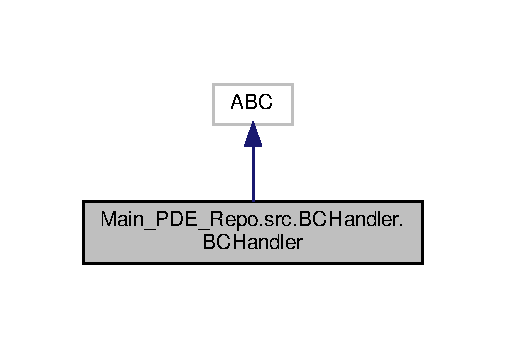
\includegraphics[width=243pt]{classMain__PDE__Repo_1_1src_1_1BCHandler_1_1BCHandler__inherit__graph}
\end{center}
\end{figure}


Collaboration diagram for Main\+\_\+\+P\+D\+E\+\_\+\+Repo.\+src.\+B\+C\+Handler.\+B\+C\+Handler\+:
\nopagebreak
\begin{figure}[H]
\begin{center}
\leavevmode
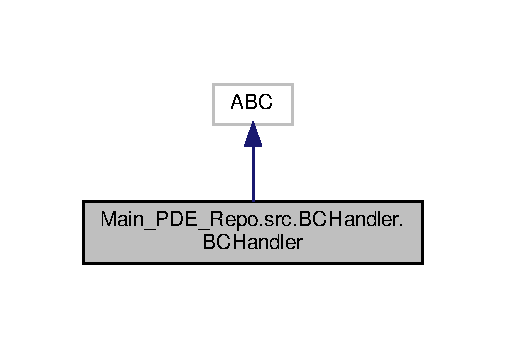
\includegraphics[width=243pt]{classMain__PDE__Repo_1_1src_1_1BCHandler_1_1BCHandler__coll__graph}
\end{center}
\end{figure}
\subsection*{Public Member Functions}
\begin{DoxyCompactItemize}
\item 
def \hyperlink{classMain__PDE__Repo_1_1src_1_1BCHandler_1_1BCHandler_a68e629dcc910ca7fe424c89ddc9d4bbe}{\+\_\+\+\_\+init\+\_\+\+\_\+} (self)
\begin{DoxyCompactList}\small\item\em The constructor. \end{DoxyCompactList}\item 
def \hyperlink{classMain__PDE__Repo_1_1src_1_1BCHandler_1_1BCHandler_a4c40f8d45a90728df43e5f583a4348de}{set\+\_\+\+B\+Cs} (self)
\begin{DoxyCompactList}\small\item\em Method to implement the contained boundary conditions. \end{DoxyCompactList}\item 
def \hyperlink{classMain__PDE__Repo_1_1src_1_1BCHandler_1_1BCHandler_aa13bfef653445fbbbec183c7e3b6277a}{check\+\_\+\+B\+Ctype} (self)
\begin{DoxyCompactList}\small\item\em Method to check if the correct type of boundary conditions have been passed to the handler. \end{DoxyCompactList}\end{DoxyCompactItemize}


\subsection{Detailed Description}
Abstract base class for implementing the P\+DE problem\textquotesingle{}s boundary conditions. 



\subsection{Constructor \& Destructor Documentation}
\mbox{\Hypertarget{classMain__PDE__Repo_1_1src_1_1BCHandler_1_1BCHandler_a68e629dcc910ca7fe424c89ddc9d4bbe}\label{classMain__PDE__Repo_1_1src_1_1BCHandler_1_1BCHandler_a68e629dcc910ca7fe424c89ddc9d4bbe}} 
\index{Main\+\_\+\+P\+D\+E\+\_\+\+Repo\+::src\+::\+B\+C\+Handler\+::\+B\+C\+Handler@{Main\+\_\+\+P\+D\+E\+\_\+\+Repo\+::src\+::\+B\+C\+Handler\+::\+B\+C\+Handler}!\+\_\+\+\_\+init\+\_\+\+\_\+@{\+\_\+\+\_\+init\+\_\+\+\_\+}}
\index{\+\_\+\+\_\+init\+\_\+\+\_\+@{\+\_\+\+\_\+init\+\_\+\+\_\+}!Main\+\_\+\+P\+D\+E\+\_\+\+Repo\+::src\+::\+B\+C\+Handler\+::\+B\+C\+Handler@{Main\+\_\+\+P\+D\+E\+\_\+\+Repo\+::src\+::\+B\+C\+Handler\+::\+B\+C\+Handler}}
\subsubsection{\texorpdfstring{\+\_\+\+\_\+init\+\_\+\+\_\+()}{\_\_init\_\_()}}
{\footnotesize\ttfamily def Main\+\_\+\+P\+D\+E\+\_\+\+Repo.\+src.\+B\+C\+Handler.\+B\+C\+Handler.\+\_\+\+\_\+init\+\_\+\+\_\+ (\begin{DoxyParamCaption}\item[{}]{self }\end{DoxyParamCaption})}



The constructor. 



\subsection{Member Function Documentation}
\mbox{\Hypertarget{classMain__PDE__Repo_1_1src_1_1BCHandler_1_1BCHandler_aa13bfef653445fbbbec183c7e3b6277a}\label{classMain__PDE__Repo_1_1src_1_1BCHandler_1_1BCHandler_aa13bfef653445fbbbec183c7e3b6277a}} 
\index{Main\+\_\+\+P\+D\+E\+\_\+\+Repo\+::src\+::\+B\+C\+Handler\+::\+B\+C\+Handler@{Main\+\_\+\+P\+D\+E\+\_\+\+Repo\+::src\+::\+B\+C\+Handler\+::\+B\+C\+Handler}!check\+\_\+\+B\+Ctype@{check\+\_\+\+B\+Ctype}}
\index{check\+\_\+\+B\+Ctype@{check\+\_\+\+B\+Ctype}!Main\+\_\+\+P\+D\+E\+\_\+\+Repo\+::src\+::\+B\+C\+Handler\+::\+B\+C\+Handler@{Main\+\_\+\+P\+D\+E\+\_\+\+Repo\+::src\+::\+B\+C\+Handler\+::\+B\+C\+Handler}}
\subsubsection{\texorpdfstring{check\+\_\+\+B\+Ctype()}{check\_BCtype()}}
{\footnotesize\ttfamily def Main\+\_\+\+P\+D\+E\+\_\+\+Repo.\+src.\+B\+C\+Handler.\+B\+C\+Handler.\+check\+\_\+\+B\+Ctype (\begin{DoxyParamCaption}\item[{}]{self }\end{DoxyParamCaption})}



Method to check if the correct type of boundary conditions have been passed to the handler. 

\mbox{\Hypertarget{classMain__PDE__Repo_1_1src_1_1BCHandler_1_1BCHandler_a4c40f8d45a90728df43e5f583a4348de}\label{classMain__PDE__Repo_1_1src_1_1BCHandler_1_1BCHandler_a4c40f8d45a90728df43e5f583a4348de}} 
\index{Main\+\_\+\+P\+D\+E\+\_\+\+Repo\+::src\+::\+B\+C\+Handler\+::\+B\+C\+Handler@{Main\+\_\+\+P\+D\+E\+\_\+\+Repo\+::src\+::\+B\+C\+Handler\+::\+B\+C\+Handler}!set\+\_\+\+B\+Cs@{set\+\_\+\+B\+Cs}}
\index{set\+\_\+\+B\+Cs@{set\+\_\+\+B\+Cs}!Main\+\_\+\+P\+D\+E\+\_\+\+Repo\+::src\+::\+B\+C\+Handler\+::\+B\+C\+Handler@{Main\+\_\+\+P\+D\+E\+\_\+\+Repo\+::src\+::\+B\+C\+Handler\+::\+B\+C\+Handler}}
\subsubsection{\texorpdfstring{set\+\_\+\+B\+Cs()}{set\_BCs()}}
{\footnotesize\ttfamily def Main\+\_\+\+P\+D\+E\+\_\+\+Repo.\+src.\+B\+C\+Handler.\+B\+C\+Handler.\+set\+\_\+\+B\+Cs (\begin{DoxyParamCaption}\item[{}]{self }\end{DoxyParamCaption})}



Method to implement the contained boundary conditions. 



The documentation for this class was generated from the following file\+:\begin{DoxyCompactItemize}
\item 
src/\hyperlink{BCHandler_8py}{B\+C\+Handler.\+py}\end{DoxyCompactItemize}

\hypertarget{classMain__PDE__Repo_1_1src_1_1BCs_1_1BCs}{}\section{Main\+\_\+\+P\+D\+E\+\_\+\+Repo.\+src.\+B\+Cs.\+B\+Cs Class Reference}
\label{classMain__PDE__Repo_1_1src_1_1BCs_1_1BCs}\index{Main\+\_\+\+P\+D\+E\+\_\+\+Repo.\+src.\+B\+Cs.\+B\+Cs@{Main\+\_\+\+P\+D\+E\+\_\+\+Repo.\+src.\+B\+Cs.\+B\+Cs}}


Abstract base class for representing the P\+DE problem\textquotesingle{}s boundary conditions.  




Inheritance diagram for Main\+\_\+\+P\+D\+E\+\_\+\+Repo.\+src.\+B\+Cs.\+B\+Cs\+:
\nopagebreak
\begin{figure}[H]
\begin{center}
\leavevmode
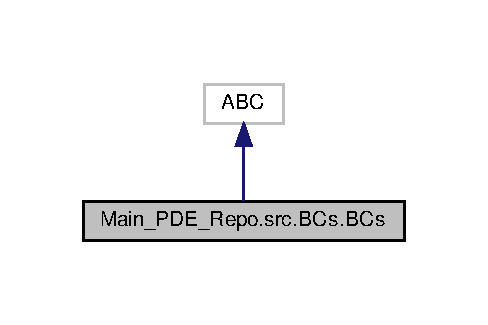
\includegraphics[width=234pt]{classMain__PDE__Repo_1_1src_1_1BCs_1_1BCs__inherit__graph}
\end{center}
\end{figure}


Collaboration diagram for Main\+\_\+\+P\+D\+E\+\_\+\+Repo.\+src.\+B\+Cs.\+B\+Cs\+:
\nopagebreak
\begin{figure}[H]
\begin{center}
\leavevmode
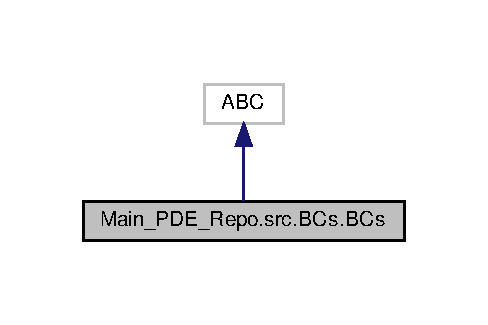
\includegraphics[width=234pt]{classMain__PDE__Repo_1_1src_1_1BCs_1_1BCs__coll__graph}
\end{center}
\end{figure}
\subsection*{Public Member Functions}
\begin{DoxyCompactItemize}
\item 
def \hyperlink{classMain__PDE__Repo_1_1src_1_1BCs_1_1BCs_a903a0a53c02b639940da31b9e90e4d0e}{\+\_\+\+\_\+init\+\_\+\+\_\+} (self)
\begin{DoxyCompactList}\small\item\em The constructor. \end{DoxyCompactList}\item 
def \hyperlink{classMain__PDE__Repo_1_1src_1_1BCs_1_1BCs_a77a1acda2d5b7301ac5ef3a883daffe2}{print\+\_\+\+B\+Cs} (self)
\begin{DoxyCompactList}\small\item\em Method to spit out the contained boundary conditions, for debugging and planning. \end{DoxyCompactList}\item 
def \hyperlink{classMain__PDE__Repo_1_1src_1_1BCs_1_1BCs_aa6cba1e1c68ddc840ee83d77575b6187}{get\+\_\+bd} (self)
\begin{DoxyCompactList}\small\item\em Method to return the boundary this boundary applies to. \end{DoxyCompactList}\item 
def \hyperlink{classMain__PDE__Repo_1_1src_1_1BCs_1_1BCs_a641fd30ccf5910519562cc4f9afc5206}{get\+\_\+bctype} (self)
\begin{DoxyCompactList}\small\item\em Method to return the type of boundary condition the object is holding. \end{DoxyCompactList}\end{DoxyCompactItemize}


\subsection{Detailed Description}
Abstract base class for representing the P\+DE problem\textquotesingle{}s boundary conditions. 



\subsection{Constructor \& Destructor Documentation}
\mbox{\Hypertarget{classMain__PDE__Repo_1_1src_1_1BCs_1_1BCs_a903a0a53c02b639940da31b9e90e4d0e}\label{classMain__PDE__Repo_1_1src_1_1BCs_1_1BCs_a903a0a53c02b639940da31b9e90e4d0e}} 
\index{Main\+\_\+\+P\+D\+E\+\_\+\+Repo\+::src\+::\+B\+Cs\+::\+B\+Cs@{Main\+\_\+\+P\+D\+E\+\_\+\+Repo\+::src\+::\+B\+Cs\+::\+B\+Cs}!\+\_\+\+\_\+init\+\_\+\+\_\+@{\+\_\+\+\_\+init\+\_\+\+\_\+}}
\index{\+\_\+\+\_\+init\+\_\+\+\_\+@{\+\_\+\+\_\+init\+\_\+\+\_\+}!Main\+\_\+\+P\+D\+E\+\_\+\+Repo\+::src\+::\+B\+Cs\+::\+B\+Cs@{Main\+\_\+\+P\+D\+E\+\_\+\+Repo\+::src\+::\+B\+Cs\+::\+B\+Cs}}
\subsubsection{\texorpdfstring{\+\_\+\+\_\+init\+\_\+\+\_\+()}{\_\_init\_\_()}}
{\footnotesize\ttfamily def Main\+\_\+\+P\+D\+E\+\_\+\+Repo.\+src.\+B\+Cs.\+B\+Cs.\+\_\+\+\_\+init\+\_\+\+\_\+ (\begin{DoxyParamCaption}\item[{}]{self }\end{DoxyParamCaption})}



The constructor. 



\subsection{Member Function Documentation}
\mbox{\Hypertarget{classMain__PDE__Repo_1_1src_1_1BCs_1_1BCs_a641fd30ccf5910519562cc4f9afc5206}\label{classMain__PDE__Repo_1_1src_1_1BCs_1_1BCs_a641fd30ccf5910519562cc4f9afc5206}} 
\index{Main\+\_\+\+P\+D\+E\+\_\+\+Repo\+::src\+::\+B\+Cs\+::\+B\+Cs@{Main\+\_\+\+P\+D\+E\+\_\+\+Repo\+::src\+::\+B\+Cs\+::\+B\+Cs}!get\+\_\+bctype@{get\+\_\+bctype}}
\index{get\+\_\+bctype@{get\+\_\+bctype}!Main\+\_\+\+P\+D\+E\+\_\+\+Repo\+::src\+::\+B\+Cs\+::\+B\+Cs@{Main\+\_\+\+P\+D\+E\+\_\+\+Repo\+::src\+::\+B\+Cs\+::\+B\+Cs}}
\subsubsection{\texorpdfstring{get\+\_\+bctype()}{get\_bctype()}}
{\footnotesize\ttfamily def Main\+\_\+\+P\+D\+E\+\_\+\+Repo.\+src.\+B\+Cs.\+B\+Cs.\+get\+\_\+bctype (\begin{DoxyParamCaption}\item[{}]{self }\end{DoxyParamCaption})}



Method to return the type of boundary condition the object is holding. 

\mbox{\Hypertarget{classMain__PDE__Repo_1_1src_1_1BCs_1_1BCs_aa6cba1e1c68ddc840ee83d77575b6187}\label{classMain__PDE__Repo_1_1src_1_1BCs_1_1BCs_aa6cba1e1c68ddc840ee83d77575b6187}} 
\index{Main\+\_\+\+P\+D\+E\+\_\+\+Repo\+::src\+::\+B\+Cs\+::\+B\+Cs@{Main\+\_\+\+P\+D\+E\+\_\+\+Repo\+::src\+::\+B\+Cs\+::\+B\+Cs}!get\+\_\+bd@{get\+\_\+bd}}
\index{get\+\_\+bd@{get\+\_\+bd}!Main\+\_\+\+P\+D\+E\+\_\+\+Repo\+::src\+::\+B\+Cs\+::\+B\+Cs@{Main\+\_\+\+P\+D\+E\+\_\+\+Repo\+::src\+::\+B\+Cs\+::\+B\+Cs}}
\subsubsection{\texorpdfstring{get\+\_\+bd()}{get\_bd()}}
{\footnotesize\ttfamily def Main\+\_\+\+P\+D\+E\+\_\+\+Repo.\+src.\+B\+Cs.\+B\+Cs.\+get\+\_\+bd (\begin{DoxyParamCaption}\item[{}]{self }\end{DoxyParamCaption})}



Method to return the boundary this boundary applies to. 

\mbox{\Hypertarget{classMain__PDE__Repo_1_1src_1_1BCs_1_1BCs_a77a1acda2d5b7301ac5ef3a883daffe2}\label{classMain__PDE__Repo_1_1src_1_1BCs_1_1BCs_a77a1acda2d5b7301ac5ef3a883daffe2}} 
\index{Main\+\_\+\+P\+D\+E\+\_\+\+Repo\+::src\+::\+B\+Cs\+::\+B\+Cs@{Main\+\_\+\+P\+D\+E\+\_\+\+Repo\+::src\+::\+B\+Cs\+::\+B\+Cs}!print\+\_\+\+B\+Cs@{print\+\_\+\+B\+Cs}}
\index{print\+\_\+\+B\+Cs@{print\+\_\+\+B\+Cs}!Main\+\_\+\+P\+D\+E\+\_\+\+Repo\+::src\+::\+B\+Cs\+::\+B\+Cs@{Main\+\_\+\+P\+D\+E\+\_\+\+Repo\+::src\+::\+B\+Cs\+::\+B\+Cs}}
\subsubsection{\texorpdfstring{print\+\_\+\+B\+Cs()}{print\_BCs()}}
{\footnotesize\ttfamily def Main\+\_\+\+P\+D\+E\+\_\+\+Repo.\+src.\+B\+Cs.\+B\+Cs.\+print\+\_\+\+B\+Cs (\begin{DoxyParamCaption}\item[{}]{self }\end{DoxyParamCaption})}



Method to spit out the contained boundary conditions, for debugging and planning. 



The documentation for this class was generated from the following file\+:\begin{DoxyCompactItemize}
\item 
src/\hyperlink{BCs_8py}{B\+Cs.\+py}\end{DoxyCompactItemize}

\hypertarget{classMain__PDE__Repo_1_1src_1_1grid_1_1CartesianGridSpec}{}\section{Main\+\_\+\+P\+D\+E\+\_\+\+Repo.\+src.\+grid.\+Cartesian\+Grid\+Spec Class Reference}
\label{classMain__PDE__Repo_1_1src_1_1grid_1_1CartesianGridSpec}\index{Main\+\_\+\+P\+D\+E\+\_\+\+Repo.\+src.\+grid.\+Cartesian\+Grid\+Spec@{Main\+\_\+\+P\+D\+E\+\_\+\+Repo.\+src.\+grid.\+Cartesian\+Grid\+Spec}}


the \hyperlink{classMain__PDE__Repo_1_1src_1_1grid_1_1CartesianGridSpec}{Cartesian\+Grid\+Spec} class  




Inheritance diagram for Main\+\_\+\+P\+D\+E\+\_\+\+Repo.\+src.\+grid.\+Cartesian\+Grid\+Spec\+:
\nopagebreak
\begin{figure}[H]
\begin{center}
\leavevmode
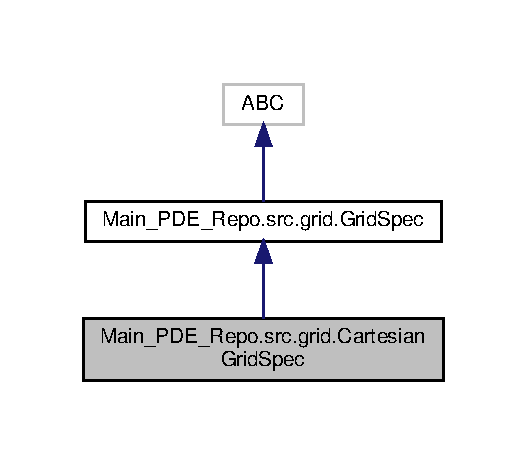
\includegraphics[width=253pt]{classMain__PDE__Repo_1_1src_1_1grid_1_1CartesianGridSpec__inherit__graph}
\end{center}
\end{figure}


Collaboration diagram for Main\+\_\+\+P\+D\+E\+\_\+\+Repo.\+src.\+grid.\+Cartesian\+Grid\+Spec\+:
\nopagebreak
\begin{figure}[H]
\begin{center}
\leavevmode
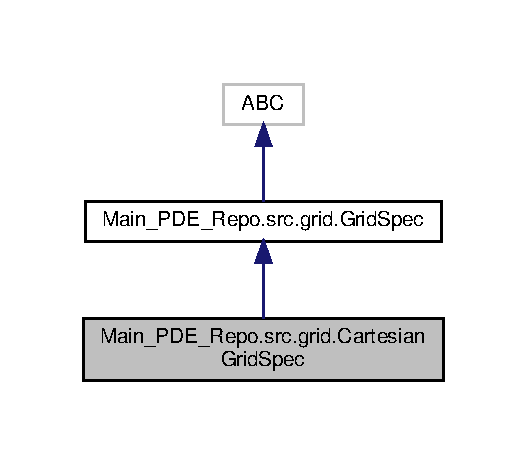
\includegraphics[width=253pt]{classMain__PDE__Repo_1_1src_1_1grid_1_1CartesianGridSpec__coll__graph}
\end{center}
\end{figure}
\subsection*{Public Member Functions}
\begin{DoxyCompactItemize}
\item 
def \hyperlink{classMain__PDE__Repo_1_1src_1_1grid_1_1CartesianGridSpec_a498dc52b08d571018cab1684316284a3}{\+\_\+\+\_\+init\+\_\+\+\_\+} (self, \hyperlink{classMain__PDE__Repo_1_1src_1_1grid_1_1CartesianGridSpec_adf422e34fb909d26139dfb3db38f9582}{coords})
\end{DoxyCompactItemize}
\subsection*{Public Attributes}
\begin{DoxyCompactItemize}
\item 
\hyperlink{classMain__PDE__Repo_1_1src_1_1grid_1_1CartesianGridSpec_adf422e34fb909d26139dfb3db38f9582}{coords}
\item 
\hyperlink{classMain__PDE__Repo_1_1src_1_1grid_1_1CartesianGridSpec_a67aedcf0f66a3c94c10bd8129011592b}{ndim}
\item 
\hyperlink{classMain__PDE__Repo_1_1src_1_1grid_1_1CartesianGridSpec_a1a5feea284988ffe55d598a93c1cc524}{gridshape}
\item 
\hyperlink{classMain__PDE__Repo_1_1src_1_1grid_1_1CartesianGridSpec_a3f6d8ebd0c81cce8fc602ff730608367}{spacing}
\end{DoxyCompactItemize}
\subsection*{Private Member Functions}
\begin{DoxyCompactItemize}
\item 
def \hyperlink{classMain__PDE__Repo_1_1src_1_1grid_1_1CartesianGridSpec_a1204b77f4cddf3247c6c07e7fc6e1b4b}{\+\_\+getspacing} (self)
\end{DoxyCompactItemize}


\subsection{Detailed Description}
the \hyperlink{classMain__PDE__Repo_1_1src_1_1grid_1_1CartesianGridSpec}{Cartesian\+Grid\+Spec} class 

\subsection{Constructor \& Destructor Documentation}
\mbox{\Hypertarget{classMain__PDE__Repo_1_1src_1_1grid_1_1CartesianGridSpec_a498dc52b08d571018cab1684316284a3}\label{classMain__PDE__Repo_1_1src_1_1grid_1_1CartesianGridSpec_a498dc52b08d571018cab1684316284a3}} 
\index{Main\+\_\+\+P\+D\+E\+\_\+\+Repo\+::src\+::grid\+::\+Cartesian\+Grid\+Spec@{Main\+\_\+\+P\+D\+E\+\_\+\+Repo\+::src\+::grid\+::\+Cartesian\+Grid\+Spec}!\+\_\+\+\_\+init\+\_\+\+\_\+@{\+\_\+\+\_\+init\+\_\+\+\_\+}}
\index{\+\_\+\+\_\+init\+\_\+\+\_\+@{\+\_\+\+\_\+init\+\_\+\+\_\+}!Main\+\_\+\+P\+D\+E\+\_\+\+Repo\+::src\+::grid\+::\+Cartesian\+Grid\+Spec@{Main\+\_\+\+P\+D\+E\+\_\+\+Repo\+::src\+::grid\+::\+Cartesian\+Grid\+Spec}}
\subsubsection{\texorpdfstring{\+\_\+\+\_\+init\+\_\+\+\_\+()}{\_\_init\_\_()}}
{\footnotesize\ttfamily def Main\+\_\+\+P\+D\+E\+\_\+\+Repo.\+src.\+grid.\+Cartesian\+Grid\+Spec.\+\_\+\+\_\+init\+\_\+\+\_\+ (\begin{DoxyParamCaption}\item[{}]{self,  }\item[{}]{coords }\end{DoxyParamCaption})}



\subsection{Member Function Documentation}
\mbox{\Hypertarget{classMain__PDE__Repo_1_1src_1_1grid_1_1CartesianGridSpec_a1204b77f4cddf3247c6c07e7fc6e1b4b}\label{classMain__PDE__Repo_1_1src_1_1grid_1_1CartesianGridSpec_a1204b77f4cddf3247c6c07e7fc6e1b4b}} 
\index{Main\+\_\+\+P\+D\+E\+\_\+\+Repo\+::src\+::grid\+::\+Cartesian\+Grid\+Spec@{Main\+\_\+\+P\+D\+E\+\_\+\+Repo\+::src\+::grid\+::\+Cartesian\+Grid\+Spec}!\+\_\+getspacing@{\+\_\+getspacing}}
\index{\+\_\+getspacing@{\+\_\+getspacing}!Main\+\_\+\+P\+D\+E\+\_\+\+Repo\+::src\+::grid\+::\+Cartesian\+Grid\+Spec@{Main\+\_\+\+P\+D\+E\+\_\+\+Repo\+::src\+::grid\+::\+Cartesian\+Grid\+Spec}}
\subsubsection{\texorpdfstring{\+\_\+getspacing()}{\_getspacing()}}
{\footnotesize\ttfamily def Main\+\_\+\+P\+D\+E\+\_\+\+Repo.\+src.\+grid.\+Cartesian\+Grid\+Spec.\+\_\+getspacing (\begin{DoxyParamCaption}\item[{}]{self }\end{DoxyParamCaption})\hspace{0.3cm}{\ttfamily [private]}}



\subsection{Member Data Documentation}
\mbox{\Hypertarget{classMain__PDE__Repo_1_1src_1_1grid_1_1CartesianGridSpec_adf422e34fb909d26139dfb3db38f9582}\label{classMain__PDE__Repo_1_1src_1_1grid_1_1CartesianGridSpec_adf422e34fb909d26139dfb3db38f9582}} 
\index{Main\+\_\+\+P\+D\+E\+\_\+\+Repo\+::src\+::grid\+::\+Cartesian\+Grid\+Spec@{Main\+\_\+\+P\+D\+E\+\_\+\+Repo\+::src\+::grid\+::\+Cartesian\+Grid\+Spec}!coords@{coords}}
\index{coords@{coords}!Main\+\_\+\+P\+D\+E\+\_\+\+Repo\+::src\+::grid\+::\+Cartesian\+Grid\+Spec@{Main\+\_\+\+P\+D\+E\+\_\+\+Repo\+::src\+::grid\+::\+Cartesian\+Grid\+Spec}}
\subsubsection{\texorpdfstring{coords}{coords}}
{\footnotesize\ttfamily Main\+\_\+\+P\+D\+E\+\_\+\+Repo.\+src.\+grid.\+Cartesian\+Grid\+Spec.\+coords}

\mbox{\Hypertarget{classMain__PDE__Repo_1_1src_1_1grid_1_1CartesianGridSpec_a1a5feea284988ffe55d598a93c1cc524}\label{classMain__PDE__Repo_1_1src_1_1grid_1_1CartesianGridSpec_a1a5feea284988ffe55d598a93c1cc524}} 
\index{Main\+\_\+\+P\+D\+E\+\_\+\+Repo\+::src\+::grid\+::\+Cartesian\+Grid\+Spec@{Main\+\_\+\+P\+D\+E\+\_\+\+Repo\+::src\+::grid\+::\+Cartesian\+Grid\+Spec}!gridshape@{gridshape}}
\index{gridshape@{gridshape}!Main\+\_\+\+P\+D\+E\+\_\+\+Repo\+::src\+::grid\+::\+Cartesian\+Grid\+Spec@{Main\+\_\+\+P\+D\+E\+\_\+\+Repo\+::src\+::grid\+::\+Cartesian\+Grid\+Spec}}
\subsubsection{\texorpdfstring{gridshape}{gridshape}}
{\footnotesize\ttfamily Main\+\_\+\+P\+D\+E\+\_\+\+Repo.\+src.\+grid.\+Cartesian\+Grid\+Spec.\+gridshape}

\mbox{\Hypertarget{classMain__PDE__Repo_1_1src_1_1grid_1_1CartesianGridSpec_a67aedcf0f66a3c94c10bd8129011592b}\label{classMain__PDE__Repo_1_1src_1_1grid_1_1CartesianGridSpec_a67aedcf0f66a3c94c10bd8129011592b}} 
\index{Main\+\_\+\+P\+D\+E\+\_\+\+Repo\+::src\+::grid\+::\+Cartesian\+Grid\+Spec@{Main\+\_\+\+P\+D\+E\+\_\+\+Repo\+::src\+::grid\+::\+Cartesian\+Grid\+Spec}!ndim@{ndim}}
\index{ndim@{ndim}!Main\+\_\+\+P\+D\+E\+\_\+\+Repo\+::src\+::grid\+::\+Cartesian\+Grid\+Spec@{Main\+\_\+\+P\+D\+E\+\_\+\+Repo\+::src\+::grid\+::\+Cartesian\+Grid\+Spec}}
\subsubsection{\texorpdfstring{ndim}{ndim}}
{\footnotesize\ttfamily Main\+\_\+\+P\+D\+E\+\_\+\+Repo.\+src.\+grid.\+Cartesian\+Grid\+Spec.\+ndim}

\mbox{\Hypertarget{classMain__PDE__Repo_1_1src_1_1grid_1_1CartesianGridSpec_a3f6d8ebd0c81cce8fc602ff730608367}\label{classMain__PDE__Repo_1_1src_1_1grid_1_1CartesianGridSpec_a3f6d8ebd0c81cce8fc602ff730608367}} 
\index{Main\+\_\+\+P\+D\+E\+\_\+\+Repo\+::src\+::grid\+::\+Cartesian\+Grid\+Spec@{Main\+\_\+\+P\+D\+E\+\_\+\+Repo\+::src\+::grid\+::\+Cartesian\+Grid\+Spec}!spacing@{spacing}}
\index{spacing@{spacing}!Main\+\_\+\+P\+D\+E\+\_\+\+Repo\+::src\+::grid\+::\+Cartesian\+Grid\+Spec@{Main\+\_\+\+P\+D\+E\+\_\+\+Repo\+::src\+::grid\+::\+Cartesian\+Grid\+Spec}}
\subsubsection{\texorpdfstring{spacing}{spacing}}
{\footnotesize\ttfamily Main\+\_\+\+P\+D\+E\+\_\+\+Repo.\+src.\+grid.\+Cartesian\+Grid\+Spec.\+spacing}



The documentation for this class was generated from the following file\+:\begin{DoxyCompactItemize}
\item 
src/\hyperlink{grid_8py}{grid.\+py}\end{DoxyCompactItemize}

\hypertarget{classMain__PDE__Repo_1_1src_1_1conduct__heat__eqn_1_1ConductHeatEqn}{}\section{Main\+\_\+\+P\+D\+E\+\_\+\+Repo.\+src.\+conduct\+\_\+heat\+\_\+eqn.\+Conduct\+Heat\+Eqn Class Reference}
\label{classMain__PDE__Repo_1_1src_1_1conduct__heat__eqn_1_1ConductHeatEqn}\index{Main\+\_\+\+P\+D\+E\+\_\+\+Repo.\+src.\+conduct\+\_\+heat\+\_\+eqn.\+Conduct\+Heat\+Eqn@{Main\+\_\+\+P\+D\+E\+\_\+\+Repo.\+src.\+conduct\+\_\+heat\+\_\+eqn.\+Conduct\+Heat\+Eqn}}


The conductive heat equation problem with no advective transport in the form d\+T/dt = alpha $\ast$ laplacian(\+T) where T is temperature and alpha is the thermal diffusivity.  




Inheritance diagram for Main\+\_\+\+P\+D\+E\+\_\+\+Repo.\+src.\+conduct\+\_\+heat\+\_\+eqn.\+Conduct\+Heat\+Eqn\+:
\nopagebreak
\begin{figure}[H]
\begin{center}
\leavevmode
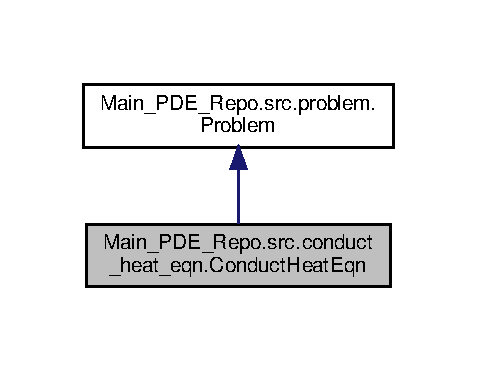
\includegraphics[width=229pt]{classMain__PDE__Repo_1_1src_1_1conduct__heat__eqn_1_1ConductHeatEqn__inherit__graph}
\end{center}
\end{figure}


Collaboration diagram for Main\+\_\+\+P\+D\+E\+\_\+\+Repo.\+src.\+conduct\+\_\+heat\+\_\+eqn.\+Conduct\+Heat\+Eqn\+:
\nopagebreak
\begin{figure}[H]
\begin{center}
\leavevmode
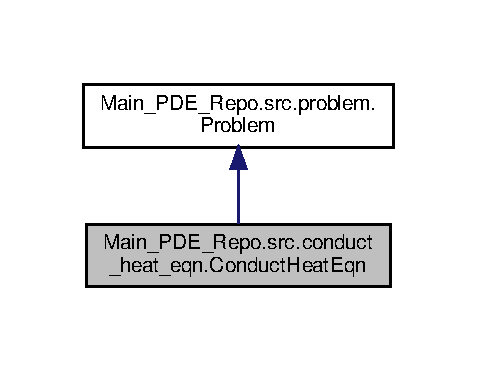
\includegraphics[width=229pt]{classMain__PDE__Repo_1_1src_1_1conduct__heat__eqn_1_1ConductHeatEqn__coll__graph}
\end{center}
\end{figure}
\subsection*{Public Member Functions}
\begin{DoxyCompactItemize}
\item 
def \hyperlink{classMain__PDE__Repo_1_1src_1_1conduct__heat__eqn_1_1ConductHeatEqn_a633aec4538eca3787158fad099fc325e}{\+\_\+\+\_\+init\+\_\+\+\_\+} (self, \hyperlink{classMain__PDE__Repo_1_1src_1_1conduct__heat__eqn_1_1ConductHeatEqn_ad02498e5299e7a1d34f9f8ef1460fddd}{boundhandl}, \hyperlink{classMain__PDE__Repo_1_1src_1_1conduct__heat__eqn_1_1ConductHeatEqn_abd7a28d699a29f455f2be1c6a8620345}{alpha}=1)
\begin{DoxyCompactList}\small\item\em The constructor. \end{DoxyCompactList}\item 
def \hyperlink{classMain__PDE__Repo_1_1src_1_1conduct__heat__eqn_1_1ConductHeatEqn_a9733763f77bf263a466bb08effec78ab}{set\+\_\+ops} (self, lin\+\_\+ops\+\_\+dict)
\begin{DoxyCompactList}\small\item\em The set\+\_\+ops function takes a dictionary of linear operators defined elsewhere and sets them to the correct member variables in the problem. \end{DoxyCompactList}\item 
def \hyperlink{classMain__PDE__Repo_1_1src_1_1conduct__heat__eqn_1_1ConductHeatEqn_a5889ab024d0a42bf84a00c1c156a19a9}{R\+HS} (self, val\+\_\+grid)
\begin{DoxyCompactList}\small\item\em The R\+HS function applies the defined operators to the grid argument in a defined manner. \end{DoxyCompactList}\item 
def \hyperlink{classMain__PDE__Repo_1_1src_1_1conduct__heat__eqn_1_1ConductHeatEqn_ac8c71907fe7365902668c6785130c522}{set\+\_\+\+B\+Cs} (self, t, val\+\_\+grid)
\begin{DoxyCompactList}\small\item\em Call the boundary handler to set the spatial boundaries to the appropriate values based on the \hyperlink{namespaceMain__PDE__Repo_1_1src_1_1BCs}{B\+Cs}. \end{DoxyCompactList}\end{DoxyCompactItemize}
\subsection*{Public Attributes}
\begin{DoxyCompactItemize}
\item 
\hyperlink{classMain__PDE__Repo_1_1src_1_1conduct__heat__eqn_1_1ConductHeatEqn_ad02498e5299e7a1d34f9f8ef1460fddd}{boundhandl}
\item 
\hyperlink{classMain__PDE__Repo_1_1src_1_1conduct__heat__eqn_1_1ConductHeatEqn_ab59c6cb80b17b0e0b17e64dffc341ec5}{ops\+\_\+set\+\_\+flag}
\item 
\hyperlink{classMain__PDE__Repo_1_1src_1_1conduct__heat__eqn_1_1ConductHeatEqn_a37601e4988c38b8a9a7f5d60867b528c}{ops}
\item 
\hyperlink{classMain__PDE__Repo_1_1src_1_1conduct__heat__eqn_1_1ConductHeatEqn_a3db974e4df85f88ce996026771f915cc}{laplacian}
\item 
\hyperlink{classMain__PDE__Repo_1_1src_1_1conduct__heat__eqn_1_1ConductHeatEqn_abd7a28d699a29f455f2be1c6a8620345}{alpha}
\end{DoxyCompactItemize}


\subsection{Detailed Description}
The conductive heat equation problem with no advective transport in the form d\+T/dt = alpha $\ast$ laplacian(\+T) where T is temperature and alpha is the thermal diffusivity. 



\subsection{Constructor \& Destructor Documentation}
\mbox{\Hypertarget{classMain__PDE__Repo_1_1src_1_1conduct__heat__eqn_1_1ConductHeatEqn_a633aec4538eca3787158fad099fc325e}\label{classMain__PDE__Repo_1_1src_1_1conduct__heat__eqn_1_1ConductHeatEqn_a633aec4538eca3787158fad099fc325e}} 
\index{Main\+\_\+\+P\+D\+E\+\_\+\+Repo\+::src\+::conduct\+\_\+heat\+\_\+eqn\+::\+Conduct\+Heat\+Eqn@{Main\+\_\+\+P\+D\+E\+\_\+\+Repo\+::src\+::conduct\+\_\+heat\+\_\+eqn\+::\+Conduct\+Heat\+Eqn}!\+\_\+\+\_\+init\+\_\+\+\_\+@{\+\_\+\+\_\+init\+\_\+\+\_\+}}
\index{\+\_\+\+\_\+init\+\_\+\+\_\+@{\+\_\+\+\_\+init\+\_\+\+\_\+}!Main\+\_\+\+P\+D\+E\+\_\+\+Repo\+::src\+::conduct\+\_\+heat\+\_\+eqn\+::\+Conduct\+Heat\+Eqn@{Main\+\_\+\+P\+D\+E\+\_\+\+Repo\+::src\+::conduct\+\_\+heat\+\_\+eqn\+::\+Conduct\+Heat\+Eqn}}
\subsubsection{\texorpdfstring{\+\_\+\+\_\+init\+\_\+\+\_\+()}{\_\_init\_\_()}}
{\footnotesize\ttfamily def Main\+\_\+\+P\+D\+E\+\_\+\+Repo.\+src.\+conduct\+\_\+heat\+\_\+eqn.\+Conduct\+Heat\+Eqn.\+\_\+\+\_\+init\+\_\+\+\_\+ (\begin{DoxyParamCaption}\item[{}]{self,  }\item[{}]{boundhandl,  }\item[{}]{alpha = {\ttfamily 1} }\end{DoxyParamCaption})}



The constructor. 


\begin{DoxyParams}{Parameters}
{\em boundhandl} & A boundary handler object \\
\hline
{\em alpha} & The value of the thermal diffusivity. Default value is 1 m$^\wedge$2/s. \\
\hline
\end{DoxyParams}


\subsection{Member Function Documentation}
\mbox{\Hypertarget{classMain__PDE__Repo_1_1src_1_1conduct__heat__eqn_1_1ConductHeatEqn_a5889ab024d0a42bf84a00c1c156a19a9}\label{classMain__PDE__Repo_1_1src_1_1conduct__heat__eqn_1_1ConductHeatEqn_a5889ab024d0a42bf84a00c1c156a19a9}} 
\index{Main\+\_\+\+P\+D\+E\+\_\+\+Repo\+::src\+::conduct\+\_\+heat\+\_\+eqn\+::\+Conduct\+Heat\+Eqn@{Main\+\_\+\+P\+D\+E\+\_\+\+Repo\+::src\+::conduct\+\_\+heat\+\_\+eqn\+::\+Conduct\+Heat\+Eqn}!R\+HS@{R\+HS}}
\index{R\+HS@{R\+HS}!Main\+\_\+\+P\+D\+E\+\_\+\+Repo\+::src\+::conduct\+\_\+heat\+\_\+eqn\+::\+Conduct\+Heat\+Eqn@{Main\+\_\+\+P\+D\+E\+\_\+\+Repo\+::src\+::conduct\+\_\+heat\+\_\+eqn\+::\+Conduct\+Heat\+Eqn}}
\subsubsection{\texorpdfstring{R\+H\+S()}{RHS()}}
{\footnotesize\ttfamily def Main\+\_\+\+P\+D\+E\+\_\+\+Repo.\+src.\+conduct\+\_\+heat\+\_\+eqn.\+Conduct\+Heat\+Eqn.\+R\+HS (\begin{DoxyParamCaption}\item[{}]{self,  }\item[{}]{val\+\_\+grid }\end{DoxyParamCaption})}



The R\+HS function applies the defined operators to the grid argument in a defined manner. 

Here the R\+HS evaluates alpha $\ast$ laplacian(val\+\_\+grid) 
\begin{DoxyParams}{Parameters}
{\em val\+\_\+grid} & The spatial grid of current values \\
\hline
\end{DoxyParams}
\begin{DoxyReturn}{Returns}
The grid containing the evaluated R\+HS values 
\end{DoxyReturn}
\mbox{\Hypertarget{classMain__PDE__Repo_1_1src_1_1conduct__heat__eqn_1_1ConductHeatEqn_ac8c71907fe7365902668c6785130c522}\label{classMain__PDE__Repo_1_1src_1_1conduct__heat__eqn_1_1ConductHeatEqn_ac8c71907fe7365902668c6785130c522}} 
\index{Main\+\_\+\+P\+D\+E\+\_\+\+Repo\+::src\+::conduct\+\_\+heat\+\_\+eqn\+::\+Conduct\+Heat\+Eqn@{Main\+\_\+\+P\+D\+E\+\_\+\+Repo\+::src\+::conduct\+\_\+heat\+\_\+eqn\+::\+Conduct\+Heat\+Eqn}!set\+\_\+\+B\+Cs@{set\+\_\+\+B\+Cs}}
\index{set\+\_\+\+B\+Cs@{set\+\_\+\+B\+Cs}!Main\+\_\+\+P\+D\+E\+\_\+\+Repo\+::src\+::conduct\+\_\+heat\+\_\+eqn\+::\+Conduct\+Heat\+Eqn@{Main\+\_\+\+P\+D\+E\+\_\+\+Repo\+::src\+::conduct\+\_\+heat\+\_\+eqn\+::\+Conduct\+Heat\+Eqn}}
\subsubsection{\texorpdfstring{set\+\_\+\+B\+Cs()}{set\_BCs()}}
{\footnotesize\ttfamily def Main\+\_\+\+P\+D\+E\+\_\+\+Repo.\+src.\+conduct\+\_\+heat\+\_\+eqn.\+Conduct\+Heat\+Eqn.\+set\+\_\+\+B\+Cs (\begin{DoxyParamCaption}\item[{}]{self,  }\item[{}]{t,  }\item[{}]{val\+\_\+grid }\end{DoxyParamCaption})}



Call the boundary handler to set the spatial boundaries to the appropriate values based on the \hyperlink{namespaceMain__PDE__Repo_1_1src_1_1BCs}{B\+Cs}. 


\begin{DoxyParams}{Parameters}
{\em t} & The current time \\
\hline
{\em val\+\_\+grid} & The spatial grid of function values \\
\hline
\end{DoxyParams}
\begin{DoxyReturn}{Returns}
Updated grid with correct boundary values 
\end{DoxyReturn}
\mbox{\Hypertarget{classMain__PDE__Repo_1_1src_1_1conduct__heat__eqn_1_1ConductHeatEqn_a9733763f77bf263a466bb08effec78ab}\label{classMain__PDE__Repo_1_1src_1_1conduct__heat__eqn_1_1ConductHeatEqn_a9733763f77bf263a466bb08effec78ab}} 
\index{Main\+\_\+\+P\+D\+E\+\_\+\+Repo\+::src\+::conduct\+\_\+heat\+\_\+eqn\+::\+Conduct\+Heat\+Eqn@{Main\+\_\+\+P\+D\+E\+\_\+\+Repo\+::src\+::conduct\+\_\+heat\+\_\+eqn\+::\+Conduct\+Heat\+Eqn}!set\+\_\+ops@{set\+\_\+ops}}
\index{set\+\_\+ops@{set\+\_\+ops}!Main\+\_\+\+P\+D\+E\+\_\+\+Repo\+::src\+::conduct\+\_\+heat\+\_\+eqn\+::\+Conduct\+Heat\+Eqn@{Main\+\_\+\+P\+D\+E\+\_\+\+Repo\+::src\+::conduct\+\_\+heat\+\_\+eqn\+::\+Conduct\+Heat\+Eqn}}
\subsubsection{\texorpdfstring{set\+\_\+ops()}{set\_ops()}}
{\footnotesize\ttfamily def Main\+\_\+\+P\+D\+E\+\_\+\+Repo.\+src.\+conduct\+\_\+heat\+\_\+eqn.\+Conduct\+Heat\+Eqn.\+set\+\_\+ops (\begin{DoxyParamCaption}\item[{}]{self,  }\item[{}]{lin\+\_\+ops\+\_\+dict }\end{DoxyParamCaption})}



The set\+\_\+ops function takes a dictionary of linear operators defined elsewhere and sets them to the correct member variables in the problem. 


\begin{DoxyParams}{Parameters}
{\em lin\+\_\+ops\+\_\+dict} & Dictionary of linear operators \\
\hline
\end{DoxyParams}


\subsection{Member Data Documentation}
\mbox{\Hypertarget{classMain__PDE__Repo_1_1src_1_1conduct__heat__eqn_1_1ConductHeatEqn_abd7a28d699a29f455f2be1c6a8620345}\label{classMain__PDE__Repo_1_1src_1_1conduct__heat__eqn_1_1ConductHeatEqn_abd7a28d699a29f455f2be1c6a8620345}} 
\index{Main\+\_\+\+P\+D\+E\+\_\+\+Repo\+::src\+::conduct\+\_\+heat\+\_\+eqn\+::\+Conduct\+Heat\+Eqn@{Main\+\_\+\+P\+D\+E\+\_\+\+Repo\+::src\+::conduct\+\_\+heat\+\_\+eqn\+::\+Conduct\+Heat\+Eqn}!alpha@{alpha}}
\index{alpha@{alpha}!Main\+\_\+\+P\+D\+E\+\_\+\+Repo\+::src\+::conduct\+\_\+heat\+\_\+eqn\+::\+Conduct\+Heat\+Eqn@{Main\+\_\+\+P\+D\+E\+\_\+\+Repo\+::src\+::conduct\+\_\+heat\+\_\+eqn\+::\+Conduct\+Heat\+Eqn}}
\subsubsection{\texorpdfstring{alpha}{alpha}}
{\footnotesize\ttfamily Main\+\_\+\+P\+D\+E\+\_\+\+Repo.\+src.\+conduct\+\_\+heat\+\_\+eqn.\+Conduct\+Heat\+Eqn.\+alpha}

\mbox{\Hypertarget{classMain__PDE__Repo_1_1src_1_1conduct__heat__eqn_1_1ConductHeatEqn_ad02498e5299e7a1d34f9f8ef1460fddd}\label{classMain__PDE__Repo_1_1src_1_1conduct__heat__eqn_1_1ConductHeatEqn_ad02498e5299e7a1d34f9f8ef1460fddd}} 
\index{Main\+\_\+\+P\+D\+E\+\_\+\+Repo\+::src\+::conduct\+\_\+heat\+\_\+eqn\+::\+Conduct\+Heat\+Eqn@{Main\+\_\+\+P\+D\+E\+\_\+\+Repo\+::src\+::conduct\+\_\+heat\+\_\+eqn\+::\+Conduct\+Heat\+Eqn}!boundhandl@{boundhandl}}
\index{boundhandl@{boundhandl}!Main\+\_\+\+P\+D\+E\+\_\+\+Repo\+::src\+::conduct\+\_\+heat\+\_\+eqn\+::\+Conduct\+Heat\+Eqn@{Main\+\_\+\+P\+D\+E\+\_\+\+Repo\+::src\+::conduct\+\_\+heat\+\_\+eqn\+::\+Conduct\+Heat\+Eqn}}
\subsubsection{\texorpdfstring{boundhandl}{boundhandl}}
{\footnotesize\ttfamily Main\+\_\+\+P\+D\+E\+\_\+\+Repo.\+src.\+conduct\+\_\+heat\+\_\+eqn.\+Conduct\+Heat\+Eqn.\+boundhandl}

\mbox{\Hypertarget{classMain__PDE__Repo_1_1src_1_1conduct__heat__eqn_1_1ConductHeatEqn_a3db974e4df85f88ce996026771f915cc}\label{classMain__PDE__Repo_1_1src_1_1conduct__heat__eqn_1_1ConductHeatEqn_a3db974e4df85f88ce996026771f915cc}} 
\index{Main\+\_\+\+P\+D\+E\+\_\+\+Repo\+::src\+::conduct\+\_\+heat\+\_\+eqn\+::\+Conduct\+Heat\+Eqn@{Main\+\_\+\+P\+D\+E\+\_\+\+Repo\+::src\+::conduct\+\_\+heat\+\_\+eqn\+::\+Conduct\+Heat\+Eqn}!laplacian@{laplacian}}
\index{laplacian@{laplacian}!Main\+\_\+\+P\+D\+E\+\_\+\+Repo\+::src\+::conduct\+\_\+heat\+\_\+eqn\+::\+Conduct\+Heat\+Eqn@{Main\+\_\+\+P\+D\+E\+\_\+\+Repo\+::src\+::conduct\+\_\+heat\+\_\+eqn\+::\+Conduct\+Heat\+Eqn}}
\subsubsection{\texorpdfstring{laplacian}{laplacian}}
{\footnotesize\ttfamily Main\+\_\+\+P\+D\+E\+\_\+\+Repo.\+src.\+conduct\+\_\+heat\+\_\+eqn.\+Conduct\+Heat\+Eqn.\+laplacian}

\mbox{\Hypertarget{classMain__PDE__Repo_1_1src_1_1conduct__heat__eqn_1_1ConductHeatEqn_a37601e4988c38b8a9a7f5d60867b528c}\label{classMain__PDE__Repo_1_1src_1_1conduct__heat__eqn_1_1ConductHeatEqn_a37601e4988c38b8a9a7f5d60867b528c}} 
\index{Main\+\_\+\+P\+D\+E\+\_\+\+Repo\+::src\+::conduct\+\_\+heat\+\_\+eqn\+::\+Conduct\+Heat\+Eqn@{Main\+\_\+\+P\+D\+E\+\_\+\+Repo\+::src\+::conduct\+\_\+heat\+\_\+eqn\+::\+Conduct\+Heat\+Eqn}!ops@{ops}}
\index{ops@{ops}!Main\+\_\+\+P\+D\+E\+\_\+\+Repo\+::src\+::conduct\+\_\+heat\+\_\+eqn\+::\+Conduct\+Heat\+Eqn@{Main\+\_\+\+P\+D\+E\+\_\+\+Repo\+::src\+::conduct\+\_\+heat\+\_\+eqn\+::\+Conduct\+Heat\+Eqn}}
\subsubsection{\texorpdfstring{ops}{ops}}
{\footnotesize\ttfamily Main\+\_\+\+P\+D\+E\+\_\+\+Repo.\+src.\+conduct\+\_\+heat\+\_\+eqn.\+Conduct\+Heat\+Eqn.\+ops}

\mbox{\Hypertarget{classMain__PDE__Repo_1_1src_1_1conduct__heat__eqn_1_1ConductHeatEqn_ab59c6cb80b17b0e0b17e64dffc341ec5}\label{classMain__PDE__Repo_1_1src_1_1conduct__heat__eqn_1_1ConductHeatEqn_ab59c6cb80b17b0e0b17e64dffc341ec5}} 
\index{Main\+\_\+\+P\+D\+E\+\_\+\+Repo\+::src\+::conduct\+\_\+heat\+\_\+eqn\+::\+Conduct\+Heat\+Eqn@{Main\+\_\+\+P\+D\+E\+\_\+\+Repo\+::src\+::conduct\+\_\+heat\+\_\+eqn\+::\+Conduct\+Heat\+Eqn}!ops\+\_\+set\+\_\+flag@{ops\+\_\+set\+\_\+flag}}
\index{ops\+\_\+set\+\_\+flag@{ops\+\_\+set\+\_\+flag}!Main\+\_\+\+P\+D\+E\+\_\+\+Repo\+::src\+::conduct\+\_\+heat\+\_\+eqn\+::\+Conduct\+Heat\+Eqn@{Main\+\_\+\+P\+D\+E\+\_\+\+Repo\+::src\+::conduct\+\_\+heat\+\_\+eqn\+::\+Conduct\+Heat\+Eqn}}
\subsubsection{\texorpdfstring{ops\+\_\+set\+\_\+flag}{ops\_set\_flag}}
{\footnotesize\ttfamily Main\+\_\+\+P\+D\+E\+\_\+\+Repo.\+src.\+conduct\+\_\+heat\+\_\+eqn.\+Conduct\+Heat\+Eqn.\+ops\+\_\+set\+\_\+flag}



The documentation for this class was generated from the following file\+:\begin{DoxyCompactItemize}
\item 
src/\hyperlink{conduct__heat__eqn_8py}{conduct\+\_\+heat\+\_\+eqn.\+py}\end{DoxyCompactItemize}

\hypertarget{classMain__PDE__Repo_1_1src_1_1static__bcs_1_1Dirichlet}{}\section{Main\+\_\+\+P\+D\+E\+\_\+\+Repo.\+src.\+static\+\_\+bcs.\+Dirichlet Class Reference}
\label{classMain__PDE__Repo_1_1src_1_1static__bcs_1_1Dirichlet}\index{Main\+\_\+\+P\+D\+E\+\_\+\+Repo.\+src.\+static\+\_\+bcs.\+Dirichlet@{Main\+\_\+\+P\+D\+E\+\_\+\+Repo.\+src.\+static\+\_\+bcs.\+Dirichlet}}


Child \hyperlink{namespaceMain__PDE__Repo_1_1src_1_1BCs}{B\+Cs} class for handling one side with static \hyperlink{classMain__PDE__Repo_1_1src_1_1static__bcs_1_1Dirichlet}{Dirichlet} boundary conditions.  




Inheritance diagram for Main\+\_\+\+P\+D\+E\+\_\+\+Repo.\+src.\+static\+\_\+bcs.\+Dirichlet\+:
\nopagebreak
\begin{figure}[H]
\begin{center}
\leavevmode
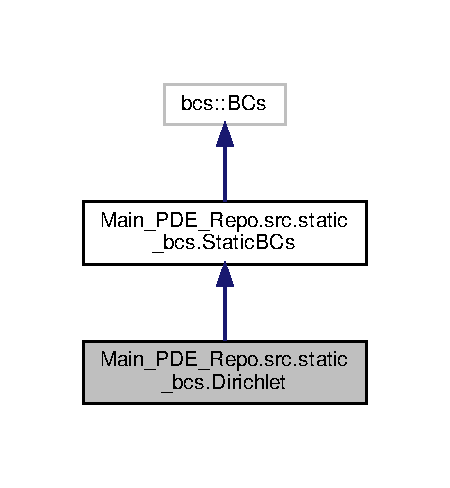
\includegraphics[width=216pt]{classMain__PDE__Repo_1_1src_1_1static__bcs_1_1Dirichlet__inherit__graph}
\end{center}
\end{figure}


Collaboration diagram for Main\+\_\+\+P\+D\+E\+\_\+\+Repo.\+src.\+static\+\_\+bcs.\+Dirichlet\+:
\nopagebreak
\begin{figure}[H]
\begin{center}
\leavevmode
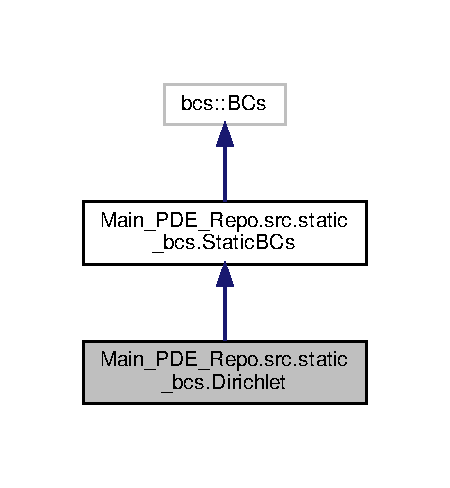
\includegraphics[width=216pt]{classMain__PDE__Repo_1_1src_1_1static__bcs_1_1Dirichlet__coll__graph}
\end{center}
\end{figure}
\subsection*{Static Public Attributes}
\begin{DoxyCompactItemize}
\item 
string \hyperlink{classMain__PDE__Repo_1_1src_1_1static__bcs_1_1Dirichlet_a20fe8b472cfabd83d02026d43a9769cf}{bctype} = \char`\"{}Dirichlet\char`\"{}
\end{DoxyCompactItemize}
\subsection*{Additional Inherited Members}


\subsection{Detailed Description}
Child \hyperlink{namespaceMain__PDE__Repo_1_1src_1_1BCs}{B\+Cs} class for handling one side with static \hyperlink{classMain__PDE__Repo_1_1src_1_1static__bcs_1_1Dirichlet}{Dirichlet} boundary conditions. 



\subsection{Member Data Documentation}
\mbox{\Hypertarget{classMain__PDE__Repo_1_1src_1_1static__bcs_1_1Dirichlet_a20fe8b472cfabd83d02026d43a9769cf}\label{classMain__PDE__Repo_1_1src_1_1static__bcs_1_1Dirichlet_a20fe8b472cfabd83d02026d43a9769cf}} 
\index{Main\+\_\+\+P\+D\+E\+\_\+\+Repo\+::src\+::static\+\_\+bcs\+::\+Dirichlet@{Main\+\_\+\+P\+D\+E\+\_\+\+Repo\+::src\+::static\+\_\+bcs\+::\+Dirichlet}!bctype@{bctype}}
\index{bctype@{bctype}!Main\+\_\+\+P\+D\+E\+\_\+\+Repo\+::src\+::static\+\_\+bcs\+::\+Dirichlet@{Main\+\_\+\+P\+D\+E\+\_\+\+Repo\+::src\+::static\+\_\+bcs\+::\+Dirichlet}}
\subsubsection{\texorpdfstring{bctype}{bctype}}
{\footnotesize\ttfamily string Main\+\_\+\+P\+D\+E\+\_\+\+Repo.\+src.\+static\+\_\+bcs.\+Dirichlet.\+bctype = \char`\"{}Dirichlet\char`\"{}\hspace{0.3cm}{\ttfamily [static]}}



The documentation for this class was generated from the following file\+:\begin{DoxyCompactItemize}
\item 
src/\hyperlink{static__bcs_8py}{static\+\_\+bcs.\+py}\end{DoxyCompactItemize}

\hypertarget{classMain__PDE__Repo_1_1src_1_1dirichlet__hand_1_1DirichletHand}{}\section{Main\+\_\+\+P\+D\+E\+\_\+\+Repo.\+src.\+dirichlet\+\_\+hand.\+Dirichlet\+Hand Class Reference}
\label{classMain__PDE__Repo_1_1src_1_1dirichlet__hand_1_1DirichletHand}\index{Main\+\_\+\+P\+D\+E\+\_\+\+Repo.\+src.\+dirichlet\+\_\+hand.\+Dirichlet\+Hand@{Main\+\_\+\+P\+D\+E\+\_\+\+Repo.\+src.\+dirichlet\+\_\+hand.\+Dirichlet\+Hand}}


Base class for implementing the P\+DE problem\textquotesingle{}s boundary conditions.  




Inheritance diagram for Main\+\_\+\+P\+D\+E\+\_\+\+Repo.\+src.\+dirichlet\+\_\+hand.\+Dirichlet\+Hand\+:
\nopagebreak
\begin{figure}[H]
\begin{center}
\leavevmode
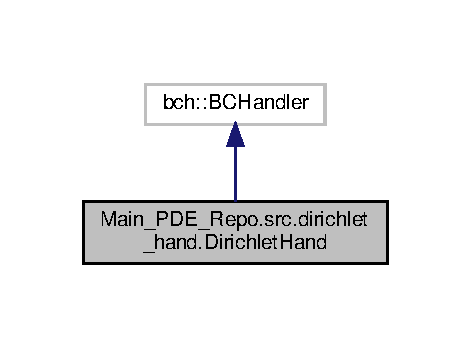
\includegraphics[width=226pt]{classMain__PDE__Repo_1_1src_1_1dirichlet__hand_1_1DirichletHand__inherit__graph}
\end{center}
\end{figure}


Collaboration diagram for Main\+\_\+\+P\+D\+E\+\_\+\+Repo.\+src.\+dirichlet\+\_\+hand.\+Dirichlet\+Hand\+:
\nopagebreak
\begin{figure}[H]
\begin{center}
\leavevmode
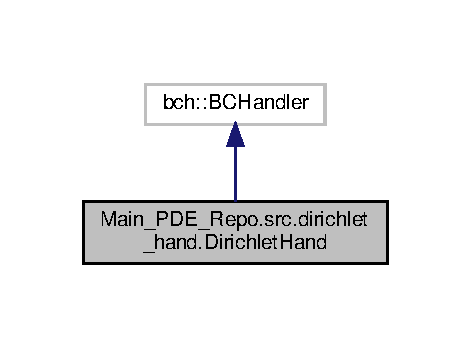
\includegraphics[width=226pt]{classMain__PDE__Repo_1_1src_1_1dirichlet__hand_1_1DirichletHand__coll__graph}
\end{center}
\end{figure}
\subsection*{Public Member Functions}
\begin{DoxyCompactItemize}
\item 
def \hyperlink{classMain__PDE__Repo_1_1src_1_1dirichlet__hand_1_1DirichletHand_a96fcbf0d3e1d031ffcd6002d2af1bdb8}{\+\_\+\+\_\+init\+\_\+\+\_\+} (self, \hyperlink{classMain__PDE__Repo_1_1src_1_1dirichlet__hand_1_1DirichletHand_aa6258cff673f06f2157191486be2d695}{bc\+\_\+list})
\item 
def \hyperlink{classMain__PDE__Repo_1_1src_1_1dirichlet__hand_1_1DirichletHand_ae37d1fb82ac443e9ef86c6f8c6c38250}{set\+\_\+\+B\+Cs} (self, time, gridqty)
\end{DoxyCompactItemize}
\subsection*{Public Attributes}
\begin{DoxyCompactItemize}
\item 
\hyperlink{classMain__PDE__Repo_1_1src_1_1dirichlet__hand_1_1DirichletHand_af2bbe35a00b6a2ef3f192e7250879c0b}{bc\+\_\+type}
\item 
\hyperlink{classMain__PDE__Repo_1_1src_1_1dirichlet__hand_1_1DirichletHand_aa6258cff673f06f2157191486be2d695}{bc\+\_\+list}
\end{DoxyCompactItemize}
\subsection*{Private Member Functions}
\begin{DoxyCompactItemize}
\item 
def \hyperlink{classMain__PDE__Repo_1_1src_1_1dirichlet__hand_1_1DirichletHand_abc40d41b239db08d96641b8ff3229efd}{\+\_\+\+B\+C\+\_\+idxs\+\_\+tuple} (self, bc, gridqty)
\item 
def \hyperlink{classMain__PDE__Repo_1_1src_1_1dirichlet__hand_1_1DirichletHand_aeaf1c49e39ac8e09dfb7195ecb6a8ced}{\+\_\+check\+\_\+\+B\+Ctype} (self)
\begin{DoxyCompactList}\small\item\em Method to check if the correct type of boundary conditions have been passed to the handler. \end{DoxyCompactList}\end{DoxyCompactItemize}


\subsection{Detailed Description}
Base class for implementing the P\+DE problem\textquotesingle{}s boundary conditions. 



\subsection{Constructor \& Destructor Documentation}
\mbox{\Hypertarget{classMain__PDE__Repo_1_1src_1_1dirichlet__hand_1_1DirichletHand_a96fcbf0d3e1d031ffcd6002d2af1bdb8}\label{classMain__PDE__Repo_1_1src_1_1dirichlet__hand_1_1DirichletHand_a96fcbf0d3e1d031ffcd6002d2af1bdb8}} 
\index{Main\+\_\+\+P\+D\+E\+\_\+\+Repo\+::src\+::dirichlet\+\_\+hand\+::\+Dirichlet\+Hand@{Main\+\_\+\+P\+D\+E\+\_\+\+Repo\+::src\+::dirichlet\+\_\+hand\+::\+Dirichlet\+Hand}!\+\_\+\+\_\+init\+\_\+\+\_\+@{\+\_\+\+\_\+init\+\_\+\+\_\+}}
\index{\+\_\+\+\_\+init\+\_\+\+\_\+@{\+\_\+\+\_\+init\+\_\+\+\_\+}!Main\+\_\+\+P\+D\+E\+\_\+\+Repo\+::src\+::dirichlet\+\_\+hand\+::\+Dirichlet\+Hand@{Main\+\_\+\+P\+D\+E\+\_\+\+Repo\+::src\+::dirichlet\+\_\+hand\+::\+Dirichlet\+Hand}}
\subsubsection{\texorpdfstring{\+\_\+\+\_\+init\+\_\+\+\_\+()}{\_\_init\_\_()}}
{\footnotesize\ttfamily def Main\+\_\+\+P\+D\+E\+\_\+\+Repo.\+src.\+dirichlet\+\_\+hand.\+Dirichlet\+Hand.\+\_\+\+\_\+init\+\_\+\+\_\+ (\begin{DoxyParamCaption}\item[{}]{self,  }\item[{}]{bc\+\_\+list }\end{DoxyParamCaption})}



\subsection{Member Function Documentation}
\mbox{\Hypertarget{classMain__PDE__Repo_1_1src_1_1dirichlet__hand_1_1DirichletHand_abc40d41b239db08d96641b8ff3229efd}\label{classMain__PDE__Repo_1_1src_1_1dirichlet__hand_1_1DirichletHand_abc40d41b239db08d96641b8ff3229efd}} 
\index{Main\+\_\+\+P\+D\+E\+\_\+\+Repo\+::src\+::dirichlet\+\_\+hand\+::\+Dirichlet\+Hand@{Main\+\_\+\+P\+D\+E\+\_\+\+Repo\+::src\+::dirichlet\+\_\+hand\+::\+Dirichlet\+Hand}!\+\_\+\+B\+C\+\_\+idxs\+\_\+tuple@{\+\_\+\+B\+C\+\_\+idxs\+\_\+tuple}}
\index{\+\_\+\+B\+C\+\_\+idxs\+\_\+tuple@{\+\_\+\+B\+C\+\_\+idxs\+\_\+tuple}!Main\+\_\+\+P\+D\+E\+\_\+\+Repo\+::src\+::dirichlet\+\_\+hand\+::\+Dirichlet\+Hand@{Main\+\_\+\+P\+D\+E\+\_\+\+Repo\+::src\+::dirichlet\+\_\+hand\+::\+Dirichlet\+Hand}}
\subsubsection{\texorpdfstring{\+\_\+\+B\+C\+\_\+idxs\+\_\+tuple()}{\_BC\_idxs\_tuple()}}
{\footnotesize\ttfamily def Main\+\_\+\+P\+D\+E\+\_\+\+Repo.\+src.\+dirichlet\+\_\+hand.\+Dirichlet\+Hand.\+\_\+\+B\+C\+\_\+idxs\+\_\+tuple (\begin{DoxyParamCaption}\item[{}]{self,  }\item[{}]{bc,  }\item[{}]{gridqty }\end{DoxyParamCaption})\hspace{0.3cm}{\ttfamily [private]}}

\mbox{\Hypertarget{classMain__PDE__Repo_1_1src_1_1dirichlet__hand_1_1DirichletHand_aeaf1c49e39ac8e09dfb7195ecb6a8ced}\label{classMain__PDE__Repo_1_1src_1_1dirichlet__hand_1_1DirichletHand_aeaf1c49e39ac8e09dfb7195ecb6a8ced}} 
\index{Main\+\_\+\+P\+D\+E\+\_\+\+Repo\+::src\+::dirichlet\+\_\+hand\+::\+Dirichlet\+Hand@{Main\+\_\+\+P\+D\+E\+\_\+\+Repo\+::src\+::dirichlet\+\_\+hand\+::\+Dirichlet\+Hand}!\+\_\+check\+\_\+\+B\+Ctype@{\+\_\+check\+\_\+\+B\+Ctype}}
\index{\+\_\+check\+\_\+\+B\+Ctype@{\+\_\+check\+\_\+\+B\+Ctype}!Main\+\_\+\+P\+D\+E\+\_\+\+Repo\+::src\+::dirichlet\+\_\+hand\+::\+Dirichlet\+Hand@{Main\+\_\+\+P\+D\+E\+\_\+\+Repo\+::src\+::dirichlet\+\_\+hand\+::\+Dirichlet\+Hand}}
\subsubsection{\texorpdfstring{\+\_\+check\+\_\+\+B\+Ctype()}{\_check\_BCtype()}}
{\footnotesize\ttfamily def Main\+\_\+\+P\+D\+E\+\_\+\+Repo.\+src.\+dirichlet\+\_\+hand.\+Dirichlet\+Hand.\+\_\+check\+\_\+\+B\+Ctype (\begin{DoxyParamCaption}\item[{}]{self }\end{DoxyParamCaption})\hspace{0.3cm}{\ttfamily [private]}}



Method to check if the correct type of boundary conditions have been passed to the handler. 

\mbox{\Hypertarget{classMain__PDE__Repo_1_1src_1_1dirichlet__hand_1_1DirichletHand_ae37d1fb82ac443e9ef86c6f8c6c38250}\label{classMain__PDE__Repo_1_1src_1_1dirichlet__hand_1_1DirichletHand_ae37d1fb82ac443e9ef86c6f8c6c38250}} 
\index{Main\+\_\+\+P\+D\+E\+\_\+\+Repo\+::src\+::dirichlet\+\_\+hand\+::\+Dirichlet\+Hand@{Main\+\_\+\+P\+D\+E\+\_\+\+Repo\+::src\+::dirichlet\+\_\+hand\+::\+Dirichlet\+Hand}!set\+\_\+\+B\+Cs@{set\+\_\+\+B\+Cs}}
\index{set\+\_\+\+B\+Cs@{set\+\_\+\+B\+Cs}!Main\+\_\+\+P\+D\+E\+\_\+\+Repo\+::src\+::dirichlet\+\_\+hand\+::\+Dirichlet\+Hand@{Main\+\_\+\+P\+D\+E\+\_\+\+Repo\+::src\+::dirichlet\+\_\+hand\+::\+Dirichlet\+Hand}}
\subsubsection{\texorpdfstring{set\+\_\+\+B\+Cs()}{set\_BCs()}}
{\footnotesize\ttfamily def Main\+\_\+\+P\+D\+E\+\_\+\+Repo.\+src.\+dirichlet\+\_\+hand.\+Dirichlet\+Hand.\+set\+\_\+\+B\+Cs (\begin{DoxyParamCaption}\item[{}]{self,  }\item[{}]{time,  }\item[{}]{gridqty }\end{DoxyParamCaption})}



\subsection{Member Data Documentation}
\mbox{\Hypertarget{classMain__PDE__Repo_1_1src_1_1dirichlet__hand_1_1DirichletHand_aa6258cff673f06f2157191486be2d695}\label{classMain__PDE__Repo_1_1src_1_1dirichlet__hand_1_1DirichletHand_aa6258cff673f06f2157191486be2d695}} 
\index{Main\+\_\+\+P\+D\+E\+\_\+\+Repo\+::src\+::dirichlet\+\_\+hand\+::\+Dirichlet\+Hand@{Main\+\_\+\+P\+D\+E\+\_\+\+Repo\+::src\+::dirichlet\+\_\+hand\+::\+Dirichlet\+Hand}!bc\+\_\+list@{bc\+\_\+list}}
\index{bc\+\_\+list@{bc\+\_\+list}!Main\+\_\+\+P\+D\+E\+\_\+\+Repo\+::src\+::dirichlet\+\_\+hand\+::\+Dirichlet\+Hand@{Main\+\_\+\+P\+D\+E\+\_\+\+Repo\+::src\+::dirichlet\+\_\+hand\+::\+Dirichlet\+Hand}}
\subsubsection{\texorpdfstring{bc\+\_\+list}{bc\_list}}
{\footnotesize\ttfamily Main\+\_\+\+P\+D\+E\+\_\+\+Repo.\+src.\+dirichlet\+\_\+hand.\+Dirichlet\+Hand.\+bc\+\_\+list}

\mbox{\Hypertarget{classMain__PDE__Repo_1_1src_1_1dirichlet__hand_1_1DirichletHand_af2bbe35a00b6a2ef3f192e7250879c0b}\label{classMain__PDE__Repo_1_1src_1_1dirichlet__hand_1_1DirichletHand_af2bbe35a00b6a2ef3f192e7250879c0b}} 
\index{Main\+\_\+\+P\+D\+E\+\_\+\+Repo\+::src\+::dirichlet\+\_\+hand\+::\+Dirichlet\+Hand@{Main\+\_\+\+P\+D\+E\+\_\+\+Repo\+::src\+::dirichlet\+\_\+hand\+::\+Dirichlet\+Hand}!bc\+\_\+type@{bc\+\_\+type}}
\index{bc\+\_\+type@{bc\+\_\+type}!Main\+\_\+\+P\+D\+E\+\_\+\+Repo\+::src\+::dirichlet\+\_\+hand\+::\+Dirichlet\+Hand@{Main\+\_\+\+P\+D\+E\+\_\+\+Repo\+::src\+::dirichlet\+\_\+hand\+::\+Dirichlet\+Hand}}
\subsubsection{\texorpdfstring{bc\+\_\+type}{bc\_type}}
{\footnotesize\ttfamily Main\+\_\+\+P\+D\+E\+\_\+\+Repo.\+src.\+dirichlet\+\_\+hand.\+Dirichlet\+Hand.\+bc\+\_\+type}



The documentation for this class was generated from the following file\+:\begin{DoxyCompactItemize}
\item 
src/\hyperlink{dirichlet__hand_8py}{dirichlet\+\_\+hand.\+py}\end{DoxyCompactItemize}

\hypertarget{classMain__PDE__Repo_1_1src_1_1driver_1_1Driver}{}\section{Main\+\_\+\+P\+D\+E\+\_\+\+Repo.\+src.\+driver.\+Driver Class Reference}
\label{classMain__PDE__Repo_1_1src_1_1driver_1_1Driver}\index{Main\+\_\+\+P\+D\+E\+\_\+\+Repo.\+src.\+driver.\+Driver@{Main\+\_\+\+P\+D\+E\+\_\+\+Repo.\+src.\+driver.\+Driver}}


The main \hyperlink{classMain__PDE__Repo_1_1src_1_1driver_1_1Driver}{Driver} class.  


\subsection*{Public Member Functions}
\begin{DoxyCompactItemize}
\item 
def \hyperlink{classMain__PDE__Repo_1_1src_1_1driver_1_1Driver_a3511ca3e52659cc97066122ff811693b}{\+\_\+\+\_\+init\+\_\+\+\_\+} (self, \hyperlink{classMain__PDE__Repo_1_1src_1_1driver_1_1Driver_afbceb17919398235d08dfa86fc9bd797}{space\+\_\+driver}, \hyperlink{classMain__PDE__Repo_1_1src_1_1driver_1_1Driver_ad203ab5d16ddeedc0717612a1d040b1e}{time\+\_\+stepper})
\begin{DoxyCompactList}\small\item\em The constructor for the \hyperlink{classMain__PDE__Repo_1_1src_1_1driver_1_1Driver}{Driver} class. \end{DoxyCompactList}\item 
def \hyperlink{classMain__PDE__Repo_1_1src_1_1driver_1_1Driver_a04fa6f2d8ec0bf649a21a9303e0dfdcf}{full\+\_\+advance} (self, t, dt, val\+\_\+grid)
\begin{DoxyCompactList}\small\item\em Advance the full probelm one time step. \end{DoxyCompactList}\item 
def \hyperlink{classMain__PDE__Repo_1_1src_1_1driver_1_1Driver_acaae71ffc87871c6873a1f348c7a396b}{full\+\_\+solve} (self, tstart, tend, dt, val\+\_\+grid)
\begin{DoxyCompactList}\small\item\em Solve the full problem for a pre-\/defined number of time steps. \end{DoxyCompactList}\end{DoxyCompactItemize}
\subsection*{Public Attributes}
\begin{DoxyCompactItemize}
\item 
\hyperlink{classMain__PDE__Repo_1_1src_1_1driver_1_1Driver_afbceb17919398235d08dfa86fc9bd797}{space\+\_\+driver}
\item 
\hyperlink{classMain__PDE__Repo_1_1src_1_1driver_1_1Driver_ad203ab5d16ddeedc0717612a1d040b1e}{time\+\_\+stepper}
\end{DoxyCompactItemize}


\subsection{Detailed Description}
The main \hyperlink{classMain__PDE__Repo_1_1src_1_1driver_1_1Driver}{Driver} class. 

\subsection{Constructor \& Destructor Documentation}
\mbox{\Hypertarget{classMain__PDE__Repo_1_1src_1_1driver_1_1Driver_a3511ca3e52659cc97066122ff811693b}\label{classMain__PDE__Repo_1_1src_1_1driver_1_1Driver_a3511ca3e52659cc97066122ff811693b}} 
\index{Main\+\_\+\+P\+D\+E\+\_\+\+Repo\+::src\+::driver\+::\+Driver@{Main\+\_\+\+P\+D\+E\+\_\+\+Repo\+::src\+::driver\+::\+Driver}!\+\_\+\+\_\+init\+\_\+\+\_\+@{\+\_\+\+\_\+init\+\_\+\+\_\+}}
\index{\+\_\+\+\_\+init\+\_\+\+\_\+@{\+\_\+\+\_\+init\+\_\+\+\_\+}!Main\+\_\+\+P\+D\+E\+\_\+\+Repo\+::src\+::driver\+::\+Driver@{Main\+\_\+\+P\+D\+E\+\_\+\+Repo\+::src\+::driver\+::\+Driver}}
\subsubsection{\texorpdfstring{\+\_\+\+\_\+init\+\_\+\+\_\+()}{\_\_init\_\_()}}
{\footnotesize\ttfamily def Main\+\_\+\+P\+D\+E\+\_\+\+Repo.\+src.\+driver.\+Driver.\+\_\+\+\_\+init\+\_\+\+\_\+ (\begin{DoxyParamCaption}\item[{}]{self,  }\item[{}]{space\+\_\+driver,  }\item[{}]{time\+\_\+stepper }\end{DoxyParamCaption})}



The constructor for the \hyperlink{classMain__PDE__Repo_1_1src_1_1driver_1_1Driver}{Driver} class. 


\begin{DoxyParams}{Parameters}
{\em space\+\_\+driver} & A Spatial\+Driver instance \\
\hline
{\em \hyperlink{namespaceMain__PDE__Repo_1_1src_1_1time__stepper}{time\+\_\+stepper}} & A Time\+Stepper instance \\
\hline
\end{DoxyParams}


\subsection{Member Function Documentation}
\mbox{\Hypertarget{classMain__PDE__Repo_1_1src_1_1driver_1_1Driver_a04fa6f2d8ec0bf649a21a9303e0dfdcf}\label{classMain__PDE__Repo_1_1src_1_1driver_1_1Driver_a04fa6f2d8ec0bf649a21a9303e0dfdcf}} 
\index{Main\+\_\+\+P\+D\+E\+\_\+\+Repo\+::src\+::driver\+::\+Driver@{Main\+\_\+\+P\+D\+E\+\_\+\+Repo\+::src\+::driver\+::\+Driver}!full\+\_\+advance@{full\+\_\+advance}}
\index{full\+\_\+advance@{full\+\_\+advance}!Main\+\_\+\+P\+D\+E\+\_\+\+Repo\+::src\+::driver\+::\+Driver@{Main\+\_\+\+P\+D\+E\+\_\+\+Repo\+::src\+::driver\+::\+Driver}}
\subsubsection{\texorpdfstring{full\+\_\+advance()}{full\_advance()}}
{\footnotesize\ttfamily def Main\+\_\+\+P\+D\+E\+\_\+\+Repo.\+src.\+driver.\+Driver.\+full\+\_\+advance (\begin{DoxyParamCaption}\item[{}]{self,  }\item[{}]{t,  }\item[{}]{dt,  }\item[{}]{val\+\_\+grid }\end{DoxyParamCaption})}



Advance the full probelm one time step. 


\begin{DoxyParams}{Parameters}
{\em t} & The current time \\
\hline
{\em dt} & The time step size \\
\hline
{\em val\+\_\+grid} & A spatial grid object \\
\hline
\end{DoxyParams}
\begin{DoxyReturn}{Returns}
The grid output from the time stepper 
\end{DoxyReturn}
\mbox{\Hypertarget{classMain__PDE__Repo_1_1src_1_1driver_1_1Driver_acaae71ffc87871c6873a1f348c7a396b}\label{classMain__PDE__Repo_1_1src_1_1driver_1_1Driver_acaae71ffc87871c6873a1f348c7a396b}} 
\index{Main\+\_\+\+P\+D\+E\+\_\+\+Repo\+::src\+::driver\+::\+Driver@{Main\+\_\+\+P\+D\+E\+\_\+\+Repo\+::src\+::driver\+::\+Driver}!full\+\_\+solve@{full\+\_\+solve}}
\index{full\+\_\+solve@{full\+\_\+solve}!Main\+\_\+\+P\+D\+E\+\_\+\+Repo\+::src\+::driver\+::\+Driver@{Main\+\_\+\+P\+D\+E\+\_\+\+Repo\+::src\+::driver\+::\+Driver}}
\subsubsection{\texorpdfstring{full\+\_\+solve()}{full\_solve()}}
{\footnotesize\ttfamily def Main\+\_\+\+P\+D\+E\+\_\+\+Repo.\+src.\+driver.\+Driver.\+full\+\_\+solve (\begin{DoxyParamCaption}\item[{}]{self,  }\item[{}]{tstart,  }\item[{}]{tend,  }\item[{}]{dt,  }\item[{}]{val\+\_\+grid }\end{DoxyParamCaption})}



Solve the full problem for a pre-\/defined number of time steps. 


\begin{DoxyParams}{Parameters}
{\em tstart} & The initial time value \\
\hline
{\em tend} & The ending time value \\
\hline
{\em dt} & The time step size \\
\hline
{\em val\+\_\+grid} & A spatial grid object \\
\hline
\end{DoxyParams}


\subsection{Member Data Documentation}
\mbox{\Hypertarget{classMain__PDE__Repo_1_1src_1_1driver_1_1Driver_afbceb17919398235d08dfa86fc9bd797}\label{classMain__PDE__Repo_1_1src_1_1driver_1_1Driver_afbceb17919398235d08dfa86fc9bd797}} 
\index{Main\+\_\+\+P\+D\+E\+\_\+\+Repo\+::src\+::driver\+::\+Driver@{Main\+\_\+\+P\+D\+E\+\_\+\+Repo\+::src\+::driver\+::\+Driver}!space\+\_\+driver@{space\+\_\+driver}}
\index{space\+\_\+driver@{space\+\_\+driver}!Main\+\_\+\+P\+D\+E\+\_\+\+Repo\+::src\+::driver\+::\+Driver@{Main\+\_\+\+P\+D\+E\+\_\+\+Repo\+::src\+::driver\+::\+Driver}}
\subsubsection{\texorpdfstring{space\+\_\+driver}{space\_driver}}
{\footnotesize\ttfamily Main\+\_\+\+P\+D\+E\+\_\+\+Repo.\+src.\+driver.\+Driver.\+space\+\_\+driver}

\mbox{\Hypertarget{classMain__PDE__Repo_1_1src_1_1driver_1_1Driver_ad203ab5d16ddeedc0717612a1d040b1e}\label{classMain__PDE__Repo_1_1src_1_1driver_1_1Driver_ad203ab5d16ddeedc0717612a1d040b1e}} 
\index{Main\+\_\+\+P\+D\+E\+\_\+\+Repo\+::src\+::driver\+::\+Driver@{Main\+\_\+\+P\+D\+E\+\_\+\+Repo\+::src\+::driver\+::\+Driver}!time\+\_\+stepper@{time\+\_\+stepper}}
\index{time\+\_\+stepper@{time\+\_\+stepper}!Main\+\_\+\+P\+D\+E\+\_\+\+Repo\+::src\+::driver\+::\+Driver@{Main\+\_\+\+P\+D\+E\+\_\+\+Repo\+::src\+::driver\+::\+Driver}}
\subsubsection{\texorpdfstring{time\+\_\+stepper}{time\_stepper}}
{\footnotesize\ttfamily Main\+\_\+\+P\+D\+E\+\_\+\+Repo.\+src.\+driver.\+Driver.\+time\+\_\+stepper}



The documentation for this class was generated from the following file\+:\begin{DoxyCompactItemize}
\item 
src/\hyperlink{driver_8py}{driver.\+py}\end{DoxyCompactItemize}

\hypertarget{classMain__PDE__Repo_1_1src_1_1edge__operator_1_1EdgeOperator}{}\section{Main\+\_\+\+P\+D\+E\+\_\+\+Repo.\+src.\+edge\+\_\+operator.\+Edge\+Operator Class Reference}
\label{classMain__PDE__Repo_1_1src_1_1edge__operator_1_1EdgeOperator}\index{Main\+\_\+\+P\+D\+E\+\_\+\+Repo.\+src.\+edge\+\_\+operator.\+Edge\+Operator@{Main\+\_\+\+P\+D\+E\+\_\+\+Repo.\+src.\+edge\+\_\+operator.\+Edge\+Operator}}


The abstract edge operator class will handle the operators applied to the edges of the grid in the evaluation of the R\+HS of the P\+DE.  




Inheritance diagram for Main\+\_\+\+P\+D\+E\+\_\+\+Repo.\+src.\+edge\+\_\+operator.\+Edge\+Operator\+:
\nopagebreak
\begin{figure}[H]
\begin{center}
\leavevmode
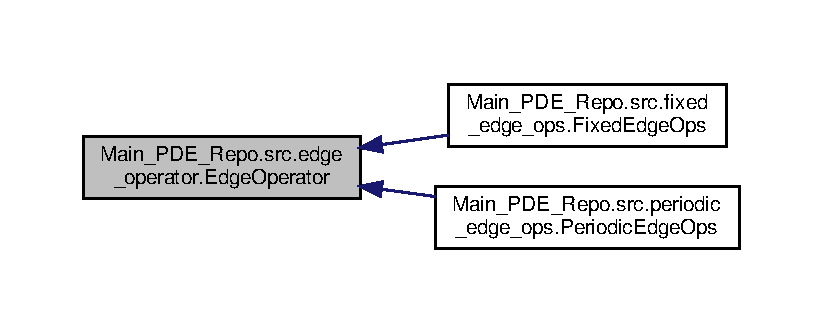
\includegraphics[width=350pt]{classMain__PDE__Repo_1_1src_1_1edge__operator_1_1EdgeOperator__inherit__graph}
\end{center}
\end{figure}
\subsection*{Public Member Functions}
\begin{DoxyCompactItemize}
\item 
def \hyperlink{classMain__PDE__Repo_1_1src_1_1edge__operator_1_1EdgeOperator_a8b441be8ab71393470f0f3e3d983889c}{\+\_\+\+\_\+init\+\_\+\+\_\+} (self)
\begin{DoxyCompactList}\small\item\em The constructor must define a name attribute. \end{DoxyCompactList}\end{DoxyCompactItemize}
\subsection*{Public Attributes}
\begin{DoxyCompactItemize}
\item 
\hyperlink{classMain__PDE__Repo_1_1src_1_1edge__operator_1_1EdgeOperator_a19f49094799db39bb5e4b218cef656eb}{name}
\end{DoxyCompactItemize}
\subsection*{Private Member Functions}
\begin{DoxyCompactItemize}
\item 
def \hyperlink{classMain__PDE__Repo_1_1src_1_1edge__operator_1_1EdgeOperator_a508247a7337a44a64100d8dc099a99c3}{\+\_\+set\+\_\+name} (self)
\begin{DoxyCompactList}\small\item\em The private method for setting the name attribute. \end{DoxyCompactList}\end{DoxyCompactItemize}


\subsection{Detailed Description}
The abstract edge operator class will handle the operators applied to the edges of the grid in the evaluation of the R\+HS of the P\+DE. 



\subsection{Constructor \& Destructor Documentation}
\mbox{\Hypertarget{classMain__PDE__Repo_1_1src_1_1edge__operator_1_1EdgeOperator_a8b441be8ab71393470f0f3e3d983889c}\label{classMain__PDE__Repo_1_1src_1_1edge__operator_1_1EdgeOperator_a8b441be8ab71393470f0f3e3d983889c}} 
\index{Main\+\_\+\+P\+D\+E\+\_\+\+Repo\+::src\+::edge\+\_\+operator\+::\+Edge\+Operator@{Main\+\_\+\+P\+D\+E\+\_\+\+Repo\+::src\+::edge\+\_\+operator\+::\+Edge\+Operator}!\+\_\+\+\_\+init\+\_\+\+\_\+@{\+\_\+\+\_\+init\+\_\+\+\_\+}}
\index{\+\_\+\+\_\+init\+\_\+\+\_\+@{\+\_\+\+\_\+init\+\_\+\+\_\+}!Main\+\_\+\+P\+D\+E\+\_\+\+Repo\+::src\+::edge\+\_\+operator\+::\+Edge\+Operator@{Main\+\_\+\+P\+D\+E\+\_\+\+Repo\+::src\+::edge\+\_\+operator\+::\+Edge\+Operator}}
\subsubsection{\texorpdfstring{\+\_\+\+\_\+init\+\_\+\+\_\+()}{\_\_init\_\_()}}
{\footnotesize\ttfamily def Main\+\_\+\+P\+D\+E\+\_\+\+Repo.\+src.\+edge\+\_\+operator.\+Edge\+Operator.\+\_\+\+\_\+init\+\_\+\+\_\+ (\begin{DoxyParamCaption}\item[{}]{self }\end{DoxyParamCaption})}



The constructor must define a name attribute. 



\subsection{Member Function Documentation}
\mbox{\Hypertarget{classMain__PDE__Repo_1_1src_1_1edge__operator_1_1EdgeOperator_a508247a7337a44a64100d8dc099a99c3}\label{classMain__PDE__Repo_1_1src_1_1edge__operator_1_1EdgeOperator_a508247a7337a44a64100d8dc099a99c3}} 
\index{Main\+\_\+\+P\+D\+E\+\_\+\+Repo\+::src\+::edge\+\_\+operator\+::\+Edge\+Operator@{Main\+\_\+\+P\+D\+E\+\_\+\+Repo\+::src\+::edge\+\_\+operator\+::\+Edge\+Operator}!\+\_\+set\+\_\+name@{\+\_\+set\+\_\+name}}
\index{\+\_\+set\+\_\+name@{\+\_\+set\+\_\+name}!Main\+\_\+\+P\+D\+E\+\_\+\+Repo\+::src\+::edge\+\_\+operator\+::\+Edge\+Operator@{Main\+\_\+\+P\+D\+E\+\_\+\+Repo\+::src\+::edge\+\_\+operator\+::\+Edge\+Operator}}
\subsubsection{\texorpdfstring{\+\_\+set\+\_\+name()}{\_set\_name()}}
{\footnotesize\ttfamily def Main\+\_\+\+P\+D\+E\+\_\+\+Repo.\+src.\+edge\+\_\+operator.\+Edge\+Operator.\+\_\+set\+\_\+name (\begin{DoxyParamCaption}\item[{}]{self }\end{DoxyParamCaption})\hspace{0.3cm}{\ttfamily [private]}}



The private method for setting the name attribute. 



\subsection{Member Data Documentation}
\mbox{\Hypertarget{classMain__PDE__Repo_1_1src_1_1edge__operator_1_1EdgeOperator_a19f49094799db39bb5e4b218cef656eb}\label{classMain__PDE__Repo_1_1src_1_1edge__operator_1_1EdgeOperator_a19f49094799db39bb5e4b218cef656eb}} 
\index{Main\+\_\+\+P\+D\+E\+\_\+\+Repo\+::src\+::edge\+\_\+operator\+::\+Edge\+Operator@{Main\+\_\+\+P\+D\+E\+\_\+\+Repo\+::src\+::edge\+\_\+operator\+::\+Edge\+Operator}!name@{name}}
\index{name@{name}!Main\+\_\+\+P\+D\+E\+\_\+\+Repo\+::src\+::edge\+\_\+operator\+::\+Edge\+Operator@{Main\+\_\+\+P\+D\+E\+\_\+\+Repo\+::src\+::edge\+\_\+operator\+::\+Edge\+Operator}}
\subsubsection{\texorpdfstring{name}{name}}
{\footnotesize\ttfamily Main\+\_\+\+P\+D\+E\+\_\+\+Repo.\+src.\+edge\+\_\+operator.\+Edge\+Operator.\+name}



The documentation for this class was generated from the following file\+:\begin{DoxyCompactItemize}
\item 
src/\hyperlink{edge__operator_8py}{edge\+\_\+operator.\+py}\end{DoxyCompactItemize}

\hypertarget{classMain__PDE__Repo_1_1src_1_1fixed__edge__ops_1_1FixedEdgeOps}{}\section{Main\+\_\+\+P\+D\+E\+\_\+\+Repo.\+src.\+fixed\+\_\+edge\+\_\+ops.\+Fixed\+Edge\+Ops Class Reference}
\label{classMain__PDE__Repo_1_1src_1_1fixed__edge__ops_1_1FixedEdgeOps}\index{Main\+\_\+\+P\+D\+E\+\_\+\+Repo.\+src.\+fixed\+\_\+edge\+\_\+ops.\+Fixed\+Edge\+Ops@{Main\+\_\+\+P\+D\+E\+\_\+\+Repo.\+src.\+fixed\+\_\+edge\+\_\+ops.\+Fixed\+Edge\+Ops}}


The fixed edge operator class handles the operators applied to the edges of the grid which correspond to fixed boundary conditions in the evaluation of the R\+HS of the P\+DE.  




Inheritance diagram for Main\+\_\+\+P\+D\+E\+\_\+\+Repo.\+src.\+fixed\+\_\+edge\+\_\+ops.\+Fixed\+Edge\+Ops\+:
\nopagebreak
\begin{figure}[H]
\begin{center}
\leavevmode
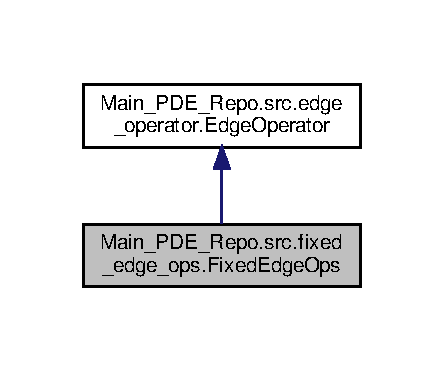
\includegraphics[width=213pt]{classMain__PDE__Repo_1_1src_1_1fixed__edge__ops_1_1FixedEdgeOps__inherit__graph}
\end{center}
\end{figure}


Collaboration diagram for Main\+\_\+\+P\+D\+E\+\_\+\+Repo.\+src.\+fixed\+\_\+edge\+\_\+ops.\+Fixed\+Edge\+Ops\+:
\nopagebreak
\begin{figure}[H]
\begin{center}
\leavevmode
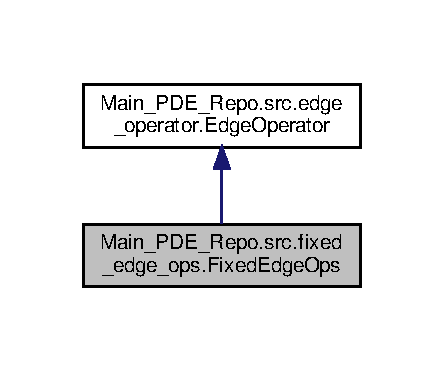
\includegraphics[width=213pt]{classMain__PDE__Repo_1_1src_1_1fixed__edge__ops_1_1FixedEdgeOps__coll__graph}
\end{center}
\end{figure}
\subsection*{Public Member Functions}
\begin{DoxyCompactItemize}
\item 
def \hyperlink{classMain__PDE__Repo_1_1src_1_1fixed__edge__ops_1_1FixedEdgeOps_a10e78a05dd1fdb424be03fa98c2ddb01}{\+\_\+\+\_\+init\+\_\+\+\_\+} (self, left\+\_\+ops\+\_\+tup, right\+\_\+ops\+\_\+tup)
\begin{DoxyCompactList}\small\item\em The constructor. \end{DoxyCompactList}\end{DoxyCompactItemize}
\subsection*{Public Attributes}
\begin{DoxyCompactItemize}
\item 
\hyperlink{classMain__PDE__Repo_1_1src_1_1fixed__edge__ops_1_1FixedEdgeOps_a91399d66e3712e6a1a2dd991d3d26e9e}{name}
\item 
\hyperlink{classMain__PDE__Repo_1_1src_1_1fixed__edge__ops_1_1FixedEdgeOps_a3297adebb84dd9e74cd5effe428a9bde}{left}
\item 
\hyperlink{classMain__PDE__Repo_1_1src_1_1fixed__edge__ops_1_1FixedEdgeOps_aea006d7915a600521621a4bb3c89f45b}{right}
\end{DoxyCompactItemize}
\subsection*{Private Member Functions}
\begin{DoxyCompactItemize}
\item 
def \hyperlink{classMain__PDE__Repo_1_1src_1_1fixed__edge__ops_1_1FixedEdgeOps_a15597526848fef9dfa96ea8e6c41c4f2}{\+\_\+set\+\_\+name} (self)
\begin{DoxyCompactList}\small\item\em Private method for setting name attribute. \end{DoxyCompactList}\end{DoxyCompactItemize}


\subsection{Detailed Description}
The fixed edge operator class handles the operators applied to the edges of the grid which correspond to fixed boundary conditions in the evaluation of the R\+HS of the P\+DE. 

The arguments are tuples of 1D operators. Each tuple corresponds to either the left (more negative) or right (more positive) edge of the axis. The operators in each tuple will be applied from the outside in, i.\+e. the first element in each tuple corresponds to the outermost edge points. 

\subsection{Constructor \& Destructor Documentation}
\mbox{\Hypertarget{classMain__PDE__Repo_1_1src_1_1fixed__edge__ops_1_1FixedEdgeOps_a10e78a05dd1fdb424be03fa98c2ddb01}\label{classMain__PDE__Repo_1_1src_1_1fixed__edge__ops_1_1FixedEdgeOps_a10e78a05dd1fdb424be03fa98c2ddb01}} 
\index{Main\+\_\+\+P\+D\+E\+\_\+\+Repo\+::src\+::fixed\+\_\+edge\+\_\+ops\+::\+Fixed\+Edge\+Ops@{Main\+\_\+\+P\+D\+E\+\_\+\+Repo\+::src\+::fixed\+\_\+edge\+\_\+ops\+::\+Fixed\+Edge\+Ops}!\+\_\+\+\_\+init\+\_\+\+\_\+@{\+\_\+\+\_\+init\+\_\+\+\_\+}}
\index{\+\_\+\+\_\+init\+\_\+\+\_\+@{\+\_\+\+\_\+init\+\_\+\+\_\+}!Main\+\_\+\+P\+D\+E\+\_\+\+Repo\+::src\+::fixed\+\_\+edge\+\_\+ops\+::\+Fixed\+Edge\+Ops@{Main\+\_\+\+P\+D\+E\+\_\+\+Repo\+::src\+::fixed\+\_\+edge\+\_\+ops\+::\+Fixed\+Edge\+Ops}}
\subsubsection{\texorpdfstring{\+\_\+\+\_\+init\+\_\+\+\_\+()}{\_\_init\_\_()}}
{\footnotesize\ttfamily def Main\+\_\+\+P\+D\+E\+\_\+\+Repo.\+src.\+fixed\+\_\+edge\+\_\+ops.\+Fixed\+Edge\+Ops.\+\_\+\+\_\+init\+\_\+\+\_\+ (\begin{DoxyParamCaption}\item[{}]{self,  }\item[{}]{left\+\_\+ops\+\_\+tup,  }\item[{}]{right\+\_\+ops\+\_\+tup }\end{DoxyParamCaption})}



The constructor. 



\subsection{Member Function Documentation}
\mbox{\Hypertarget{classMain__PDE__Repo_1_1src_1_1fixed__edge__ops_1_1FixedEdgeOps_a15597526848fef9dfa96ea8e6c41c4f2}\label{classMain__PDE__Repo_1_1src_1_1fixed__edge__ops_1_1FixedEdgeOps_a15597526848fef9dfa96ea8e6c41c4f2}} 
\index{Main\+\_\+\+P\+D\+E\+\_\+\+Repo\+::src\+::fixed\+\_\+edge\+\_\+ops\+::\+Fixed\+Edge\+Ops@{Main\+\_\+\+P\+D\+E\+\_\+\+Repo\+::src\+::fixed\+\_\+edge\+\_\+ops\+::\+Fixed\+Edge\+Ops}!\+\_\+set\+\_\+name@{\+\_\+set\+\_\+name}}
\index{\+\_\+set\+\_\+name@{\+\_\+set\+\_\+name}!Main\+\_\+\+P\+D\+E\+\_\+\+Repo\+::src\+::fixed\+\_\+edge\+\_\+ops\+::\+Fixed\+Edge\+Ops@{Main\+\_\+\+P\+D\+E\+\_\+\+Repo\+::src\+::fixed\+\_\+edge\+\_\+ops\+::\+Fixed\+Edge\+Ops}}
\subsubsection{\texorpdfstring{\+\_\+set\+\_\+name()}{\_set\_name()}}
{\footnotesize\ttfamily def Main\+\_\+\+P\+D\+E\+\_\+\+Repo.\+src.\+fixed\+\_\+edge\+\_\+ops.\+Fixed\+Edge\+Ops.\+\_\+set\+\_\+name (\begin{DoxyParamCaption}\item[{}]{self }\end{DoxyParamCaption})\hspace{0.3cm}{\ttfamily [private]}}



Private method for setting name attribute. 



\subsection{Member Data Documentation}
\mbox{\Hypertarget{classMain__PDE__Repo_1_1src_1_1fixed__edge__ops_1_1FixedEdgeOps_a3297adebb84dd9e74cd5effe428a9bde}\label{classMain__PDE__Repo_1_1src_1_1fixed__edge__ops_1_1FixedEdgeOps_a3297adebb84dd9e74cd5effe428a9bde}} 
\index{Main\+\_\+\+P\+D\+E\+\_\+\+Repo\+::src\+::fixed\+\_\+edge\+\_\+ops\+::\+Fixed\+Edge\+Ops@{Main\+\_\+\+P\+D\+E\+\_\+\+Repo\+::src\+::fixed\+\_\+edge\+\_\+ops\+::\+Fixed\+Edge\+Ops}!left@{left}}
\index{left@{left}!Main\+\_\+\+P\+D\+E\+\_\+\+Repo\+::src\+::fixed\+\_\+edge\+\_\+ops\+::\+Fixed\+Edge\+Ops@{Main\+\_\+\+P\+D\+E\+\_\+\+Repo\+::src\+::fixed\+\_\+edge\+\_\+ops\+::\+Fixed\+Edge\+Ops}}
\subsubsection{\texorpdfstring{left}{left}}
{\footnotesize\ttfamily Main\+\_\+\+P\+D\+E\+\_\+\+Repo.\+src.\+fixed\+\_\+edge\+\_\+ops.\+Fixed\+Edge\+Ops.\+left}

\mbox{\Hypertarget{classMain__PDE__Repo_1_1src_1_1fixed__edge__ops_1_1FixedEdgeOps_a91399d66e3712e6a1a2dd991d3d26e9e}\label{classMain__PDE__Repo_1_1src_1_1fixed__edge__ops_1_1FixedEdgeOps_a91399d66e3712e6a1a2dd991d3d26e9e}} 
\index{Main\+\_\+\+P\+D\+E\+\_\+\+Repo\+::src\+::fixed\+\_\+edge\+\_\+ops\+::\+Fixed\+Edge\+Ops@{Main\+\_\+\+P\+D\+E\+\_\+\+Repo\+::src\+::fixed\+\_\+edge\+\_\+ops\+::\+Fixed\+Edge\+Ops}!name@{name}}
\index{name@{name}!Main\+\_\+\+P\+D\+E\+\_\+\+Repo\+::src\+::fixed\+\_\+edge\+\_\+ops\+::\+Fixed\+Edge\+Ops@{Main\+\_\+\+P\+D\+E\+\_\+\+Repo\+::src\+::fixed\+\_\+edge\+\_\+ops\+::\+Fixed\+Edge\+Ops}}
\subsubsection{\texorpdfstring{name}{name}}
{\footnotesize\ttfamily Main\+\_\+\+P\+D\+E\+\_\+\+Repo.\+src.\+fixed\+\_\+edge\+\_\+ops.\+Fixed\+Edge\+Ops.\+name}

\mbox{\Hypertarget{classMain__PDE__Repo_1_1src_1_1fixed__edge__ops_1_1FixedEdgeOps_aea006d7915a600521621a4bb3c89f45b}\label{classMain__PDE__Repo_1_1src_1_1fixed__edge__ops_1_1FixedEdgeOps_aea006d7915a600521621a4bb3c89f45b}} 
\index{Main\+\_\+\+P\+D\+E\+\_\+\+Repo\+::src\+::fixed\+\_\+edge\+\_\+ops\+::\+Fixed\+Edge\+Ops@{Main\+\_\+\+P\+D\+E\+\_\+\+Repo\+::src\+::fixed\+\_\+edge\+\_\+ops\+::\+Fixed\+Edge\+Ops}!right@{right}}
\index{right@{right}!Main\+\_\+\+P\+D\+E\+\_\+\+Repo\+::src\+::fixed\+\_\+edge\+\_\+ops\+::\+Fixed\+Edge\+Ops@{Main\+\_\+\+P\+D\+E\+\_\+\+Repo\+::src\+::fixed\+\_\+edge\+\_\+ops\+::\+Fixed\+Edge\+Ops}}
\subsubsection{\texorpdfstring{right}{right}}
{\footnotesize\ttfamily Main\+\_\+\+P\+D\+E\+\_\+\+Repo.\+src.\+fixed\+\_\+edge\+\_\+ops.\+Fixed\+Edge\+Ops.\+right}



The documentation for this class was generated from the following file\+:\begin{DoxyCompactItemize}
\item 
src/\hyperlink{fixed__edge__ops_8py}{fixed\+\_\+edge\+\_\+ops.\+py}\end{DoxyCompactItemize}

\hypertarget{classMain__PDE__Repo_1_1src_1_1forward__euler_1_1ForwardEuler}{}\section{Main\+\_\+\+P\+D\+E\+\_\+\+Repo.\+src.\+forward\+\_\+euler.\+Forward\+Euler Class Reference}
\label{classMain__PDE__Repo_1_1src_1_1forward__euler_1_1ForwardEuler}\index{Main\+\_\+\+P\+D\+E\+\_\+\+Repo.\+src.\+forward\+\_\+euler.\+Forward\+Euler@{Main\+\_\+\+P\+D\+E\+\_\+\+Repo.\+src.\+forward\+\_\+euler.\+Forward\+Euler}}


A concrete Forward Euler subclass of Time\+Stepper.  




Inheritance diagram for Main\+\_\+\+P\+D\+E\+\_\+\+Repo.\+src.\+forward\+\_\+euler.\+Forward\+Euler\+:
\nopagebreak
\begin{figure}[H]
\begin{center}
\leavevmode
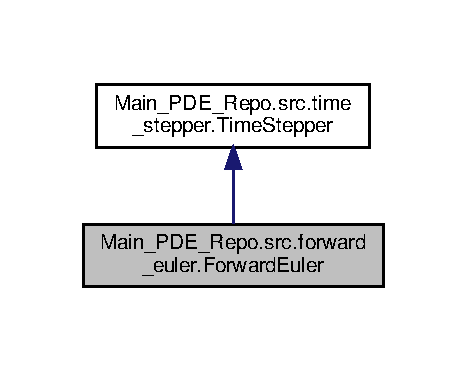
\includegraphics[width=224pt]{classMain__PDE__Repo_1_1src_1_1forward__euler_1_1ForwardEuler__inherit__graph}
\end{center}
\end{figure}


Collaboration diagram for Main\+\_\+\+P\+D\+E\+\_\+\+Repo.\+src.\+forward\+\_\+euler.\+Forward\+Euler\+:
\nopagebreak
\begin{figure}[H]
\begin{center}
\leavevmode
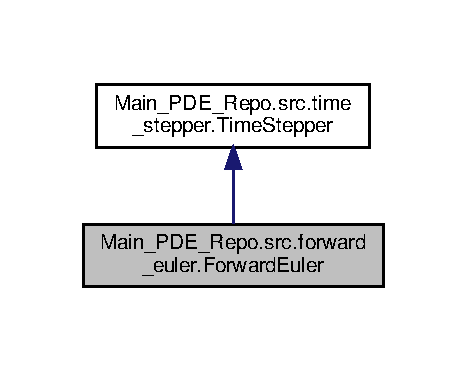
\includegraphics[width=224pt]{classMain__PDE__Repo_1_1src_1_1forward__euler_1_1ForwardEuler__coll__graph}
\end{center}
\end{figure}
\subsection*{Public Member Functions}
\begin{DoxyCompactItemize}
\item 
def \hyperlink{classMain__PDE__Repo_1_1src_1_1forward__euler_1_1ForwardEuler_aafec83c8cc54107baf7aa842563199b0}{step} (self, val\+\_\+grid, rhs\+\_\+grid, dt)
\begin{DoxyCompactList}\small\item\em The step method of the Forward Euler class. \end{DoxyCompactList}\item 
def \hyperlink{classMain__PDE__Repo_1_1src_1_1forward__euler_1_1ForwardEuler_aebafa27619dffaadc2f9b1c7f6240892}{get\+\_\+num\+\_\+grid\+\_\+elems} (self, grid\+\_\+obj)
\begin{DoxyCompactList}\small\item\em A method for determining the number of elements in a grid. \end{DoxyCompactList}\end{DoxyCompactItemize}


\subsection{Detailed Description}
A concrete Forward Euler subclass of Time\+Stepper. 

The Forward Euler method uses a simple forward finite difference approach to estimate a value at the next time step. This is done with the approximation \{u(t+dt) -\/ u(t)\}/dt = R\+HS which can be rearranged to give u(t+dt) = u(t) + dt$\ast$\+R\+HS. 

\subsection{Member Function Documentation}
\mbox{\Hypertarget{classMain__PDE__Repo_1_1src_1_1forward__euler_1_1ForwardEuler_aebafa27619dffaadc2f9b1c7f6240892}\label{classMain__PDE__Repo_1_1src_1_1forward__euler_1_1ForwardEuler_aebafa27619dffaadc2f9b1c7f6240892}} 
\index{Main\+\_\+\+P\+D\+E\+\_\+\+Repo\+::src\+::forward\+\_\+euler\+::\+Forward\+Euler@{Main\+\_\+\+P\+D\+E\+\_\+\+Repo\+::src\+::forward\+\_\+euler\+::\+Forward\+Euler}!get\+\_\+num\+\_\+grid\+\_\+elems@{get\+\_\+num\+\_\+grid\+\_\+elems}}
\index{get\+\_\+num\+\_\+grid\+\_\+elems@{get\+\_\+num\+\_\+grid\+\_\+elems}!Main\+\_\+\+P\+D\+E\+\_\+\+Repo\+::src\+::forward\+\_\+euler\+::\+Forward\+Euler@{Main\+\_\+\+P\+D\+E\+\_\+\+Repo\+::src\+::forward\+\_\+euler\+::\+Forward\+Euler}}
\subsubsection{\texorpdfstring{get\+\_\+num\+\_\+grid\+\_\+elems()}{get\_num\_grid\_elems()}}
{\footnotesize\ttfamily def Main\+\_\+\+P\+D\+E\+\_\+\+Repo.\+src.\+forward\+\_\+euler.\+Forward\+Euler.\+get\+\_\+num\+\_\+grid\+\_\+elems (\begin{DoxyParamCaption}\item[{}]{self,  }\item[{}]{grid\+\_\+obj }\end{DoxyParamCaption})}



A method for determining the number of elements in a grid. 

This is just the product of the spatial dimensions of the grid. 
\begin{DoxyParams}{Parameters}
{\em grid\+\_\+obj} & The grid to be querried \\
\hline
\end{DoxyParams}
\begin{DoxyReturn}{Returns}
The number of elements in the grid 
\end{DoxyReturn}
\mbox{\Hypertarget{classMain__PDE__Repo_1_1src_1_1forward__euler_1_1ForwardEuler_aafec83c8cc54107baf7aa842563199b0}\label{classMain__PDE__Repo_1_1src_1_1forward__euler_1_1ForwardEuler_aafec83c8cc54107baf7aa842563199b0}} 
\index{Main\+\_\+\+P\+D\+E\+\_\+\+Repo\+::src\+::forward\+\_\+euler\+::\+Forward\+Euler@{Main\+\_\+\+P\+D\+E\+\_\+\+Repo\+::src\+::forward\+\_\+euler\+::\+Forward\+Euler}!step@{step}}
\index{step@{step}!Main\+\_\+\+P\+D\+E\+\_\+\+Repo\+::src\+::forward\+\_\+euler\+::\+Forward\+Euler@{Main\+\_\+\+P\+D\+E\+\_\+\+Repo\+::src\+::forward\+\_\+euler\+::\+Forward\+Euler}}
\subsubsection{\texorpdfstring{step()}{step()}}
{\footnotesize\ttfamily def Main\+\_\+\+P\+D\+E\+\_\+\+Repo.\+src.\+forward\+\_\+euler.\+Forward\+Euler.\+step (\begin{DoxyParamCaption}\item[{}]{self,  }\item[{}]{val\+\_\+grid,  }\item[{}]{rhs\+\_\+grid,  }\item[{}]{dt }\end{DoxyParamCaption})}



The step method of the Forward Euler class. 

Implements the basic Forward Euler algorithm on the input grid object. 
\begin{DoxyParams}{Parameters}
{\em val\+\_\+grid} & The spatial grid of values at the current time \\
\hline
{\em rhs\+\_\+grid} & The spatial grid of R\+HS values \\
\hline
{\em dt} & The time step size \\
\hline
\end{DoxyParams}
\begin{DoxyReturn}{Returns}
Spatial grid with new values for the next time step 
\end{DoxyReturn}


The documentation for this class was generated from the following file\+:\begin{DoxyCompactItemize}
\item 
src/\hyperlink{forward__euler_8py}{forward\+\_\+euler.\+py}\end{DoxyCompactItemize}

\hypertarget{classMain__PDE__Repo_1_1src_1_1gridoperator_1_1GridOperator}{}\section{Main\+\_\+\+P\+D\+E\+\_\+\+Repo.\+src.\+gridoperator.\+Grid\+Operator Class Reference}
\label{classMain__PDE__Repo_1_1src_1_1gridoperator_1_1GridOperator}\index{Main\+\_\+\+P\+D\+E\+\_\+\+Repo.\+src.\+gridoperator.\+Grid\+Operator@{Main\+\_\+\+P\+D\+E\+\_\+\+Repo.\+src.\+gridoperator.\+Grid\+Operator}}


\hyperlink{classMain__PDE__Repo_1_1src_1_1gridoperator_1_1GridOperator}{Grid\+Operator} \hyperlink{classMain__PDE__Repo_1_1src_1_1gridoperator_1_1GridOperator}{Grid\+Operator} class definition.  


\subsection*{Public Member Functions}
\begin{DoxyCompactItemize}
\item 
def \hyperlink{classMain__PDE__Repo_1_1src_1_1gridoperator_1_1GridOperator_a874aaa760371b08e21431b13fd615dfc}{\+\_\+\+\_\+init\+\_\+\+\_\+} (self, \hyperlink{classMain__PDE__Repo_1_1src_1_1gridoperator_1_1GridOperator_a4fb567c3ca465539b3a726f7532dc0ee}{spec}, \hyperlink{classMain__PDE__Repo_1_1src_1_1gridoperator_1_1GridOperator_aa6270af360bec9b3331951328b48a724}{ndscheme})
\item 
def \hyperlink{classMain__PDE__Repo_1_1src_1_1gridoperator_1_1GridOperator_a9794669e62dbcafb6ecd7e687a5e75b5}{\+\_\+\+\_\+call\+\_\+\+\_\+} (self, grid)
\begin{DoxyCompactList}\small\item\em {\bfseries call} Evaluate the scalar version of the grid operator on a given grid \end{DoxyCompactList}\end{DoxyCompactItemize}
\subsection*{Public Attributes}
\begin{DoxyCompactItemize}
\item 
\hyperlink{classMain__PDE__Repo_1_1src_1_1gridoperator_1_1GridOperator_a4fb567c3ca465539b3a726f7532dc0ee}{spec}
\item 
\hyperlink{classMain__PDE__Repo_1_1src_1_1gridoperator_1_1GridOperator_aa6270af360bec9b3331951328b48a724}{ndscheme}
\item 
\hyperlink{classMain__PDE__Repo_1_1src_1_1gridoperator_1_1GridOperator_aed5a97e2a911c29b47523c6a072e4720}{opmats}
\item 
\hyperlink{classMain__PDE__Repo_1_1src_1_1gridoperator_1_1GridOperator_a1091ae0b853c4ae1b7fdb734dcb7d4af}{basemesh}
\item 
\hyperlink{classMain__PDE__Repo_1_1src_1_1gridoperator_1_1GridOperator_a2d253ceb81a2b90bc7b7e1231aeb79c5}{N}
\item 
\hyperlink{classMain__PDE__Repo_1_1src_1_1gridoperator_1_1GridOperator_ae92052af91aaaefda0465ae51d816100}{scalar\+\_\+op}
\end{DoxyCompactItemize}
\subsection*{Private Member Functions}
\begin{DoxyCompactItemize}
\item 
def \hyperlink{classMain__PDE__Repo_1_1src_1_1gridoperator_1_1GridOperator_a1dcfb3ac8b3fe0c540a6ef788ea5f0a1}{\+\_\+get\+\_\+\+Int} (self, op1d, size)
\item 
def \hyperlink{classMain__PDE__Repo_1_1src_1_1gridoperator_1_1GridOperator_a33da253271c9dcc762ba0e728453d77e}{\+\_\+apply\+\_\+op} (self, popul, opmat, op1d, slc)
\item 
def \hyperlink{classMain__PDE__Repo_1_1src_1_1gridoperator_1_1GridOperator_ab0568659ff00ab8eb6249eb188bc00eb}{\+\_\+bl\+\_\+set} (self, popul, opmat, edgeop, layer\+\_\+dim, \hyperlink{classMain__PDE__Repo_1_1src_1_1gridoperator_1_1GridOperator_a2d253ceb81a2b90bc7b7e1231aeb79c5}{N})
\end{DoxyCompactItemize}


\subsection{Detailed Description}
\hyperlink{classMain__PDE__Repo_1_1src_1_1gridoperator_1_1GridOperator}{Grid\+Operator} \hyperlink{classMain__PDE__Repo_1_1src_1_1gridoperator_1_1GridOperator}{Grid\+Operator} class definition. 

\subsection{Constructor \& Destructor Documentation}
\mbox{\Hypertarget{classMain__PDE__Repo_1_1src_1_1gridoperator_1_1GridOperator_a874aaa760371b08e21431b13fd615dfc}\label{classMain__PDE__Repo_1_1src_1_1gridoperator_1_1GridOperator_a874aaa760371b08e21431b13fd615dfc}} 
\index{Main\+\_\+\+P\+D\+E\+\_\+\+Repo\+::src\+::gridoperator\+::\+Grid\+Operator@{Main\+\_\+\+P\+D\+E\+\_\+\+Repo\+::src\+::gridoperator\+::\+Grid\+Operator}!\+\_\+\+\_\+init\+\_\+\+\_\+@{\+\_\+\+\_\+init\+\_\+\+\_\+}}
\index{\+\_\+\+\_\+init\+\_\+\+\_\+@{\+\_\+\+\_\+init\+\_\+\+\_\+}!Main\+\_\+\+P\+D\+E\+\_\+\+Repo\+::src\+::gridoperator\+::\+Grid\+Operator@{Main\+\_\+\+P\+D\+E\+\_\+\+Repo\+::src\+::gridoperator\+::\+Grid\+Operator}}
\subsubsection{\texorpdfstring{\+\_\+\+\_\+init\+\_\+\+\_\+()}{\_\_init\_\_()}}
{\footnotesize\ttfamily def Main\+\_\+\+P\+D\+E\+\_\+\+Repo.\+src.\+gridoperator.\+Grid\+Operator.\+\_\+\+\_\+init\+\_\+\+\_\+ (\begin{DoxyParamCaption}\item[{}]{self,  }\item[{}]{spec,  }\item[{}]{ndscheme }\end{DoxyParamCaption})}



\subsection{Member Function Documentation}
\mbox{\Hypertarget{classMain__PDE__Repo_1_1src_1_1gridoperator_1_1GridOperator_a9794669e62dbcafb6ecd7e687a5e75b5}\label{classMain__PDE__Repo_1_1src_1_1gridoperator_1_1GridOperator_a9794669e62dbcafb6ecd7e687a5e75b5}} 
\index{Main\+\_\+\+P\+D\+E\+\_\+\+Repo\+::src\+::gridoperator\+::\+Grid\+Operator@{Main\+\_\+\+P\+D\+E\+\_\+\+Repo\+::src\+::gridoperator\+::\+Grid\+Operator}!\+\_\+\+\_\+call\+\_\+\+\_\+@{\+\_\+\+\_\+call\+\_\+\+\_\+}}
\index{\+\_\+\+\_\+call\+\_\+\+\_\+@{\+\_\+\+\_\+call\+\_\+\+\_\+}!Main\+\_\+\+P\+D\+E\+\_\+\+Repo\+::src\+::gridoperator\+::\+Grid\+Operator@{Main\+\_\+\+P\+D\+E\+\_\+\+Repo\+::src\+::gridoperator\+::\+Grid\+Operator}}
\subsubsection{\texorpdfstring{\+\_\+\+\_\+call\+\_\+\+\_\+()}{\_\_call\_\_()}}
{\footnotesize\ttfamily def Main\+\_\+\+P\+D\+E\+\_\+\+Repo.\+src.\+gridoperator.\+Grid\+Operator.\+\_\+\+\_\+call\+\_\+\+\_\+ (\begin{DoxyParamCaption}\item[{}]{self,  }\item[{}]{grid }\end{DoxyParamCaption})}



{\bfseries call} Evaluate the scalar version of the grid operator on a given grid 

Take a gridqty object of arbitrary dimension and apply the gridoperator object to each scalar contained in the grid Return a new gridqty object of the same type and size with the values corresponding to the 
\begin{DoxyParams}{Parameters}
{\em grid} & a Grid\+Qty object \\
\hline
\end{DoxyParams}
\mbox{\Hypertarget{classMain__PDE__Repo_1_1src_1_1gridoperator_1_1GridOperator_a33da253271c9dcc762ba0e728453d77e}\label{classMain__PDE__Repo_1_1src_1_1gridoperator_1_1GridOperator_a33da253271c9dcc762ba0e728453d77e}} 
\index{Main\+\_\+\+P\+D\+E\+\_\+\+Repo\+::src\+::gridoperator\+::\+Grid\+Operator@{Main\+\_\+\+P\+D\+E\+\_\+\+Repo\+::src\+::gridoperator\+::\+Grid\+Operator}!\+\_\+apply\+\_\+op@{\+\_\+apply\+\_\+op}}
\index{\+\_\+apply\+\_\+op@{\+\_\+apply\+\_\+op}!Main\+\_\+\+P\+D\+E\+\_\+\+Repo\+::src\+::gridoperator\+::\+Grid\+Operator@{Main\+\_\+\+P\+D\+E\+\_\+\+Repo\+::src\+::gridoperator\+::\+Grid\+Operator}}
\subsubsection{\texorpdfstring{\+\_\+apply\+\_\+op()}{\_apply\_op()}}
{\footnotesize\ttfamily def Main\+\_\+\+P\+D\+E\+\_\+\+Repo.\+src.\+gridoperator.\+Grid\+Operator.\+\_\+apply\+\_\+op (\begin{DoxyParamCaption}\item[{}]{self,  }\item[{}]{popul,  }\item[{}]{opmat,  }\item[{}]{op1d,  }\item[{}]{slc }\end{DoxyParamCaption})\hspace{0.3cm}{\ttfamily [private]}}

\mbox{\Hypertarget{classMain__PDE__Repo_1_1src_1_1gridoperator_1_1GridOperator_ab0568659ff00ab8eb6249eb188bc00eb}\label{classMain__PDE__Repo_1_1src_1_1gridoperator_1_1GridOperator_ab0568659ff00ab8eb6249eb188bc00eb}} 
\index{Main\+\_\+\+P\+D\+E\+\_\+\+Repo\+::src\+::gridoperator\+::\+Grid\+Operator@{Main\+\_\+\+P\+D\+E\+\_\+\+Repo\+::src\+::gridoperator\+::\+Grid\+Operator}!\+\_\+bl\+\_\+set@{\+\_\+bl\+\_\+set}}
\index{\+\_\+bl\+\_\+set@{\+\_\+bl\+\_\+set}!Main\+\_\+\+P\+D\+E\+\_\+\+Repo\+::src\+::gridoperator\+::\+Grid\+Operator@{Main\+\_\+\+P\+D\+E\+\_\+\+Repo\+::src\+::gridoperator\+::\+Grid\+Operator}}
\subsubsection{\texorpdfstring{\+\_\+bl\+\_\+set()}{\_bl\_set()}}
{\footnotesize\ttfamily def Main\+\_\+\+P\+D\+E\+\_\+\+Repo.\+src.\+gridoperator.\+Grid\+Operator.\+\_\+bl\+\_\+set (\begin{DoxyParamCaption}\item[{}]{self,  }\item[{}]{popul,  }\item[{}]{opmat,  }\item[{}]{edgeop,  }\item[{}]{layer\+\_\+dim,  }\item[{}]{N }\end{DoxyParamCaption})\hspace{0.3cm}{\ttfamily [private]}}

\mbox{\Hypertarget{classMain__PDE__Repo_1_1src_1_1gridoperator_1_1GridOperator_a1dcfb3ac8b3fe0c540a6ef788ea5f0a1}\label{classMain__PDE__Repo_1_1src_1_1gridoperator_1_1GridOperator_a1dcfb3ac8b3fe0c540a6ef788ea5f0a1}} 
\index{Main\+\_\+\+P\+D\+E\+\_\+\+Repo\+::src\+::gridoperator\+::\+Grid\+Operator@{Main\+\_\+\+P\+D\+E\+\_\+\+Repo\+::src\+::gridoperator\+::\+Grid\+Operator}!\+\_\+get\+\_\+\+Int@{\+\_\+get\+\_\+\+Int}}
\index{\+\_\+get\+\_\+\+Int@{\+\_\+get\+\_\+\+Int}!Main\+\_\+\+P\+D\+E\+\_\+\+Repo\+::src\+::gridoperator\+::\+Grid\+Operator@{Main\+\_\+\+P\+D\+E\+\_\+\+Repo\+::src\+::gridoperator\+::\+Grid\+Operator}}
\subsubsection{\texorpdfstring{\+\_\+get\+\_\+\+Int()}{\_get\_Int()}}
{\footnotesize\ttfamily def Main\+\_\+\+P\+D\+E\+\_\+\+Repo.\+src.\+gridoperator.\+Grid\+Operator.\+\_\+get\+\_\+\+Int (\begin{DoxyParamCaption}\item[{}]{self,  }\item[{}]{op1d,  }\item[{}]{size }\end{DoxyParamCaption})\hspace{0.3cm}{\ttfamily [private]}}



\subsection{Member Data Documentation}
\mbox{\Hypertarget{classMain__PDE__Repo_1_1src_1_1gridoperator_1_1GridOperator_a1091ae0b853c4ae1b7fdb734dcb7d4af}\label{classMain__PDE__Repo_1_1src_1_1gridoperator_1_1GridOperator_a1091ae0b853c4ae1b7fdb734dcb7d4af}} 
\index{Main\+\_\+\+P\+D\+E\+\_\+\+Repo\+::src\+::gridoperator\+::\+Grid\+Operator@{Main\+\_\+\+P\+D\+E\+\_\+\+Repo\+::src\+::gridoperator\+::\+Grid\+Operator}!basemesh@{basemesh}}
\index{basemesh@{basemesh}!Main\+\_\+\+P\+D\+E\+\_\+\+Repo\+::src\+::gridoperator\+::\+Grid\+Operator@{Main\+\_\+\+P\+D\+E\+\_\+\+Repo\+::src\+::gridoperator\+::\+Grid\+Operator}}
\subsubsection{\texorpdfstring{basemesh}{basemesh}}
{\footnotesize\ttfamily Main\+\_\+\+P\+D\+E\+\_\+\+Repo.\+src.\+gridoperator.\+Grid\+Operator.\+basemesh}

\mbox{\Hypertarget{classMain__PDE__Repo_1_1src_1_1gridoperator_1_1GridOperator_a2d253ceb81a2b90bc7b7e1231aeb79c5}\label{classMain__PDE__Repo_1_1src_1_1gridoperator_1_1GridOperator_a2d253ceb81a2b90bc7b7e1231aeb79c5}} 
\index{Main\+\_\+\+P\+D\+E\+\_\+\+Repo\+::src\+::gridoperator\+::\+Grid\+Operator@{Main\+\_\+\+P\+D\+E\+\_\+\+Repo\+::src\+::gridoperator\+::\+Grid\+Operator}!N@{N}}
\index{N@{N}!Main\+\_\+\+P\+D\+E\+\_\+\+Repo\+::src\+::gridoperator\+::\+Grid\+Operator@{Main\+\_\+\+P\+D\+E\+\_\+\+Repo\+::src\+::gridoperator\+::\+Grid\+Operator}}
\subsubsection{\texorpdfstring{N}{N}}
{\footnotesize\ttfamily Main\+\_\+\+P\+D\+E\+\_\+\+Repo.\+src.\+gridoperator.\+Grid\+Operator.\+N}

\mbox{\Hypertarget{classMain__PDE__Repo_1_1src_1_1gridoperator_1_1GridOperator_aa6270af360bec9b3331951328b48a724}\label{classMain__PDE__Repo_1_1src_1_1gridoperator_1_1GridOperator_aa6270af360bec9b3331951328b48a724}} 
\index{Main\+\_\+\+P\+D\+E\+\_\+\+Repo\+::src\+::gridoperator\+::\+Grid\+Operator@{Main\+\_\+\+P\+D\+E\+\_\+\+Repo\+::src\+::gridoperator\+::\+Grid\+Operator}!ndscheme@{ndscheme}}
\index{ndscheme@{ndscheme}!Main\+\_\+\+P\+D\+E\+\_\+\+Repo\+::src\+::gridoperator\+::\+Grid\+Operator@{Main\+\_\+\+P\+D\+E\+\_\+\+Repo\+::src\+::gridoperator\+::\+Grid\+Operator}}
\subsubsection{\texorpdfstring{ndscheme}{ndscheme}}
{\footnotesize\ttfamily Main\+\_\+\+P\+D\+E\+\_\+\+Repo.\+src.\+gridoperator.\+Grid\+Operator.\+ndscheme}

\mbox{\Hypertarget{classMain__PDE__Repo_1_1src_1_1gridoperator_1_1GridOperator_aed5a97e2a911c29b47523c6a072e4720}\label{classMain__PDE__Repo_1_1src_1_1gridoperator_1_1GridOperator_aed5a97e2a911c29b47523c6a072e4720}} 
\index{Main\+\_\+\+P\+D\+E\+\_\+\+Repo\+::src\+::gridoperator\+::\+Grid\+Operator@{Main\+\_\+\+P\+D\+E\+\_\+\+Repo\+::src\+::gridoperator\+::\+Grid\+Operator}!opmats@{opmats}}
\index{opmats@{opmats}!Main\+\_\+\+P\+D\+E\+\_\+\+Repo\+::src\+::gridoperator\+::\+Grid\+Operator@{Main\+\_\+\+P\+D\+E\+\_\+\+Repo\+::src\+::gridoperator\+::\+Grid\+Operator}}
\subsubsection{\texorpdfstring{opmats}{opmats}}
{\footnotesize\ttfamily Main\+\_\+\+P\+D\+E\+\_\+\+Repo.\+src.\+gridoperator.\+Grid\+Operator.\+opmats}

\mbox{\Hypertarget{classMain__PDE__Repo_1_1src_1_1gridoperator_1_1GridOperator_ae92052af91aaaefda0465ae51d816100}\label{classMain__PDE__Repo_1_1src_1_1gridoperator_1_1GridOperator_ae92052af91aaaefda0465ae51d816100}} 
\index{Main\+\_\+\+P\+D\+E\+\_\+\+Repo\+::src\+::gridoperator\+::\+Grid\+Operator@{Main\+\_\+\+P\+D\+E\+\_\+\+Repo\+::src\+::gridoperator\+::\+Grid\+Operator}!scalar\+\_\+op@{scalar\+\_\+op}}
\index{scalar\+\_\+op@{scalar\+\_\+op}!Main\+\_\+\+P\+D\+E\+\_\+\+Repo\+::src\+::gridoperator\+::\+Grid\+Operator@{Main\+\_\+\+P\+D\+E\+\_\+\+Repo\+::src\+::gridoperator\+::\+Grid\+Operator}}
\subsubsection{\texorpdfstring{scalar\+\_\+op}{scalar\_op}}
{\footnotesize\ttfamily Main\+\_\+\+P\+D\+E\+\_\+\+Repo.\+src.\+gridoperator.\+Grid\+Operator.\+scalar\+\_\+op}

\mbox{\Hypertarget{classMain__PDE__Repo_1_1src_1_1gridoperator_1_1GridOperator_a4fb567c3ca465539b3a726f7532dc0ee}\label{classMain__PDE__Repo_1_1src_1_1gridoperator_1_1GridOperator_a4fb567c3ca465539b3a726f7532dc0ee}} 
\index{Main\+\_\+\+P\+D\+E\+\_\+\+Repo\+::src\+::gridoperator\+::\+Grid\+Operator@{Main\+\_\+\+P\+D\+E\+\_\+\+Repo\+::src\+::gridoperator\+::\+Grid\+Operator}!spec@{spec}}
\index{spec@{spec}!Main\+\_\+\+P\+D\+E\+\_\+\+Repo\+::src\+::gridoperator\+::\+Grid\+Operator@{Main\+\_\+\+P\+D\+E\+\_\+\+Repo\+::src\+::gridoperator\+::\+Grid\+Operator}}
\subsubsection{\texorpdfstring{spec}{spec}}
{\footnotesize\ttfamily Main\+\_\+\+P\+D\+E\+\_\+\+Repo.\+src.\+gridoperator.\+Grid\+Operator.\+spec}



The documentation for this class was generated from the following file\+:\begin{DoxyCompactItemize}
\item 
src/\hyperlink{gridoperator_8py}{gridoperator.\+py}\end{DoxyCompactItemize}

\hypertarget{classMain__PDE__Repo_1_1src_1_1grid_1_1GridQty}{}\section{Main\+\_\+\+P\+D\+E\+\_\+\+Repo.\+src.\+grid.\+Grid\+Qty Class Reference}
\label{classMain__PDE__Repo_1_1src_1_1grid_1_1GridQty}\index{Main\+\_\+\+P\+D\+E\+\_\+\+Repo.\+src.\+grid.\+Grid\+Qty@{Main\+\_\+\+P\+D\+E\+\_\+\+Repo.\+src.\+grid.\+Grid\+Qty}}


The \hyperlink{classMain__PDE__Repo_1_1src_1_1grid_1_1GridQty}{Grid\+Qty} abstract base class.  




Inheritance diagram for Main\+\_\+\+P\+D\+E\+\_\+\+Repo.\+src.\+grid.\+Grid\+Qty\+:
\nopagebreak
\begin{figure}[H]
\begin{center}
\leavevmode
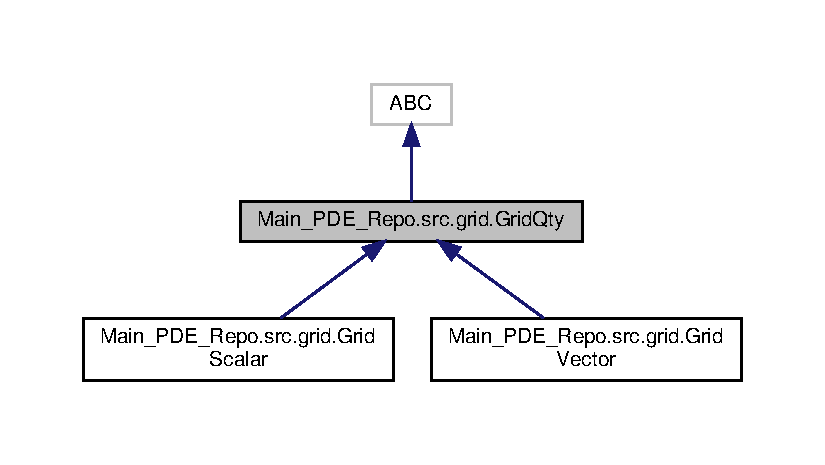
\includegraphics[width=350pt]{classMain__PDE__Repo_1_1src_1_1grid_1_1GridQty__inherit__graph}
\end{center}
\end{figure}


Collaboration diagram for Main\+\_\+\+P\+D\+E\+\_\+\+Repo.\+src.\+grid.\+Grid\+Qty\+:
\nopagebreak
\begin{figure}[H]
\begin{center}
\leavevmode
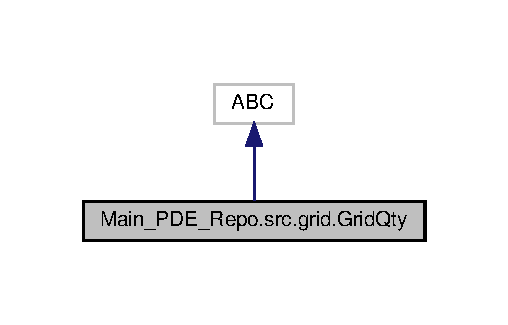
\includegraphics[width=244pt]{classMain__PDE__Repo_1_1src_1_1grid_1_1GridQty__coll__graph}
\end{center}
\end{figure}
\subsection*{Public Member Functions}
\begin{DoxyCompactItemize}
\item 
def \hyperlink{classMain__PDE__Repo_1_1src_1_1grid_1_1GridQty_a9adaebfb98afe1a1074e9aad8d6ca879}{\+\_\+\+\_\+init\+\_\+\+\_\+} (self, \hyperlink{classMain__PDE__Repo_1_1src_1_1grid_1_1GridQty_af8f206d6eb9037737417e4fefb52990e}{spec}, initial\+\_\+vals)
\item 
def \hyperlink{classMain__PDE__Repo_1_1src_1_1grid_1_1GridQty_ab9b199129e09cd0f959e553292a75015}{\+\_\+\+\_\+getattr\+\_\+\+\_\+} (self, attr)
\begin{DoxyCompactList}\small\item\em Getattr method\+: If a method isn\textquotesingle{}t specified for a \hyperlink{classMain__PDE__Repo_1_1src_1_1grid_1_1GridQty}{Grid\+Qty} object, instead try doing operations on the grid attribute. \end{DoxyCompactList}\item 
def \hyperlink{classMain__PDE__Repo_1_1src_1_1grid_1_1GridQty_a5080f35125b0d132cc1226d7967996bb}{getslice} (self, indices, squeeze=False)
\begin{DoxyCompactList}\small\item\em Getslice method. \end{DoxyCompactList}\item 
def \hyperlink{classMain__PDE__Repo_1_1src_1_1grid_1_1GridQty_a991e5653e03be1daeabfd5dd512fd75c}{setslice} (self, indices, values)
\begin{DoxyCompactList}\small\item\em Setslice method. \end{DoxyCompactList}\end{DoxyCompactItemize}
\subsection*{Public Attributes}
\begin{DoxyCompactItemize}
\item 
\hyperlink{classMain__PDE__Repo_1_1src_1_1grid_1_1GridQty_af8f206d6eb9037737417e4fefb52990e}{spec}
\item 
\hyperlink{classMain__PDE__Repo_1_1src_1_1grid_1_1GridQty_ad506c5469e4f07ccdcd1cca7239d1555}{gqshape}
\begin{DoxyCompactList}\small\item\em The constructor for the \hyperlink{classMain__PDE__Repo_1_1src_1_1grid_1_1GridQty}{Grid\+Qty}. \end{DoxyCompactList}\item 
\hyperlink{classMain__PDE__Repo_1_1src_1_1grid_1_1GridQty_a78259425113459873f41c8ece6d05c1c}{grid}
\end{DoxyCompactItemize}
\subsection*{Private Member Functions}
\begin{DoxyCompactItemize}
\item 
def \hyperlink{classMain__PDE__Repo_1_1src_1_1grid_1_1GridQty_a0c68e16bd939efac875a60f539bb66f6}{\+\_\+qtyshape} (self)
\begin{DoxyCompactList}\small\item\em Abstract method \+\_\+qtyshape, to return the dimensions of the stored object (versus the \hyperlink{classMain__PDE__Repo_1_1src_1_1grid_1_1GridSpec}{Grid\+Spec}) A non-\/abstract child must override each abstract method inherited from its parent by defining a method with the same signature and same return type. \end{DoxyCompactList}\end{DoxyCompactItemize}
\subsection*{Static Private Member Functions}
\begin{DoxyCompactItemize}
\item 
def \hyperlink{classMain__PDE__Repo_1_1src_1_1grid_1_1GridQty_af7f9a9ebb90e4911e7292e721f7d1de9}{\+\_\+makegrid} (shape, initial\+\_\+vals, kwargs)
\begin{DoxyCompactList}\small\item\em Static method \+\_\+makegrid $\ast$$\ast$kwards\+: whatever keywords that also want to include in the grid static method that is agnostic to the particular child class calling it. \end{DoxyCompactList}\item 
def \hyperlink{classMain__PDE__Repo_1_1src_1_1grid_1_1GridQty_a048ff999254cfe9420fd377a6edc289b}{\+\_\+indexify} (indices)
\begin{DoxyCompactList}\small\item\em \+\_\+indexify method for use by getslice and setslice methods Static method knows nothing about the class and just deals with the parameters. \end{DoxyCompactList}\end{DoxyCompactItemize}


\subsection{Detailed Description}
The \hyperlink{classMain__PDE__Repo_1_1src_1_1grid_1_1GridQty}{Grid\+Qty} abstract base class. 

\subsection{Constructor \& Destructor Documentation}
\mbox{\Hypertarget{classMain__PDE__Repo_1_1src_1_1grid_1_1GridQty_a9adaebfb98afe1a1074e9aad8d6ca879}\label{classMain__PDE__Repo_1_1src_1_1grid_1_1GridQty_a9adaebfb98afe1a1074e9aad8d6ca879}} 
\index{Main\+\_\+\+P\+D\+E\+\_\+\+Repo\+::src\+::grid\+::\+Grid\+Qty@{Main\+\_\+\+P\+D\+E\+\_\+\+Repo\+::src\+::grid\+::\+Grid\+Qty}!\+\_\+\+\_\+init\+\_\+\+\_\+@{\+\_\+\+\_\+init\+\_\+\+\_\+}}
\index{\+\_\+\+\_\+init\+\_\+\+\_\+@{\+\_\+\+\_\+init\+\_\+\+\_\+}!Main\+\_\+\+P\+D\+E\+\_\+\+Repo\+::src\+::grid\+::\+Grid\+Qty@{Main\+\_\+\+P\+D\+E\+\_\+\+Repo\+::src\+::grid\+::\+Grid\+Qty}}
\subsubsection{\texorpdfstring{\+\_\+\+\_\+init\+\_\+\+\_\+()}{\_\_init\_\_()}}
{\footnotesize\ttfamily def Main\+\_\+\+P\+D\+E\+\_\+\+Repo.\+src.\+grid.\+Grid\+Qty.\+\_\+\+\_\+init\+\_\+\+\_\+ (\begin{DoxyParamCaption}\item[{}]{self,  }\item[{}]{spec,  }\item[{}]{initial\+\_\+vals }\end{DoxyParamCaption})}



\subsection{Member Function Documentation}
\mbox{\Hypertarget{classMain__PDE__Repo_1_1src_1_1grid_1_1GridQty_ab9b199129e09cd0f959e553292a75015}\label{classMain__PDE__Repo_1_1src_1_1grid_1_1GridQty_ab9b199129e09cd0f959e553292a75015}} 
\index{Main\+\_\+\+P\+D\+E\+\_\+\+Repo\+::src\+::grid\+::\+Grid\+Qty@{Main\+\_\+\+P\+D\+E\+\_\+\+Repo\+::src\+::grid\+::\+Grid\+Qty}!\+\_\+\+\_\+getattr\+\_\+\+\_\+@{\+\_\+\+\_\+getattr\+\_\+\+\_\+}}
\index{\+\_\+\+\_\+getattr\+\_\+\+\_\+@{\+\_\+\+\_\+getattr\+\_\+\+\_\+}!Main\+\_\+\+P\+D\+E\+\_\+\+Repo\+::src\+::grid\+::\+Grid\+Qty@{Main\+\_\+\+P\+D\+E\+\_\+\+Repo\+::src\+::grid\+::\+Grid\+Qty}}
\subsubsection{\texorpdfstring{\+\_\+\+\_\+getattr\+\_\+\+\_\+()}{\_\_getattr\_\_()}}
{\footnotesize\ttfamily def Main\+\_\+\+P\+D\+E\+\_\+\+Repo.\+src.\+grid.\+Grid\+Qty.\+\_\+\+\_\+getattr\+\_\+\+\_\+ (\begin{DoxyParamCaption}\item[{}]{self,  }\item[{}]{attr }\end{DoxyParamCaption})}



Getattr method\+: If a method isn\textquotesingle{}t specified for a \hyperlink{classMain__PDE__Repo_1_1src_1_1grid_1_1GridQty}{Grid\+Qty} object, instead try doing operations on the grid attribute. 


\begin{DoxyParams}{Parameters}
{\em attr} & The attribute of \hyperlink{classMain__PDE__Repo_1_1src_1_1grid_1_1GridQty}{Grid\+Qty} we are attempting to reference \\
\hline
\end{DoxyParams}
\mbox{\Hypertarget{classMain__PDE__Repo_1_1src_1_1grid_1_1GridQty_a048ff999254cfe9420fd377a6edc289b}\label{classMain__PDE__Repo_1_1src_1_1grid_1_1GridQty_a048ff999254cfe9420fd377a6edc289b}} 
\index{Main\+\_\+\+P\+D\+E\+\_\+\+Repo\+::src\+::grid\+::\+Grid\+Qty@{Main\+\_\+\+P\+D\+E\+\_\+\+Repo\+::src\+::grid\+::\+Grid\+Qty}!\+\_\+indexify@{\+\_\+indexify}}
\index{\+\_\+indexify@{\+\_\+indexify}!Main\+\_\+\+P\+D\+E\+\_\+\+Repo\+::src\+::grid\+::\+Grid\+Qty@{Main\+\_\+\+P\+D\+E\+\_\+\+Repo\+::src\+::grid\+::\+Grid\+Qty}}
\subsubsection{\texorpdfstring{\+\_\+indexify()}{\_indexify()}}
{\footnotesize\ttfamily def Main\+\_\+\+P\+D\+E\+\_\+\+Repo.\+src.\+grid.\+Grid\+Qty.\+\_\+indexify (\begin{DoxyParamCaption}\item[{}]{indices }\end{DoxyParamCaption})\hspace{0.3cm}{\ttfamily [static]}, {\ttfamily [private]}}



\+\_\+indexify method for use by getslice and setslice methods Static method knows nothing about the class and just deals with the parameters. 

\mbox{\Hypertarget{classMain__PDE__Repo_1_1src_1_1grid_1_1GridQty_af7f9a9ebb90e4911e7292e721f7d1de9}\label{classMain__PDE__Repo_1_1src_1_1grid_1_1GridQty_af7f9a9ebb90e4911e7292e721f7d1de9}} 
\index{Main\+\_\+\+P\+D\+E\+\_\+\+Repo\+::src\+::grid\+::\+Grid\+Qty@{Main\+\_\+\+P\+D\+E\+\_\+\+Repo\+::src\+::grid\+::\+Grid\+Qty}!\+\_\+makegrid@{\+\_\+makegrid}}
\index{\+\_\+makegrid@{\+\_\+makegrid}!Main\+\_\+\+P\+D\+E\+\_\+\+Repo\+::src\+::grid\+::\+Grid\+Qty@{Main\+\_\+\+P\+D\+E\+\_\+\+Repo\+::src\+::grid\+::\+Grid\+Qty}}
\subsubsection{\texorpdfstring{\+\_\+makegrid()}{\_makegrid()}}
{\footnotesize\ttfamily def Main\+\_\+\+P\+D\+E\+\_\+\+Repo.\+src.\+grid.\+Grid\+Qty.\+\_\+makegrid (\begin{DoxyParamCaption}\item[{}]{shape,  }\item[{}]{initial\+\_\+vals,  }\item[{}]{kwargs }\end{DoxyParamCaption})\hspace{0.3cm}{\ttfamily [static]}, {\ttfamily [private]}}



Static method \+\_\+makegrid $\ast$$\ast$kwards\+: whatever keywords that also want to include in the grid static method that is agnostic to the particular child class calling it. 

\mbox{\Hypertarget{classMain__PDE__Repo_1_1src_1_1grid_1_1GridQty_a0c68e16bd939efac875a60f539bb66f6}\label{classMain__PDE__Repo_1_1src_1_1grid_1_1GridQty_a0c68e16bd939efac875a60f539bb66f6}} 
\index{Main\+\_\+\+P\+D\+E\+\_\+\+Repo\+::src\+::grid\+::\+Grid\+Qty@{Main\+\_\+\+P\+D\+E\+\_\+\+Repo\+::src\+::grid\+::\+Grid\+Qty}!\+\_\+qtyshape@{\+\_\+qtyshape}}
\index{\+\_\+qtyshape@{\+\_\+qtyshape}!Main\+\_\+\+P\+D\+E\+\_\+\+Repo\+::src\+::grid\+::\+Grid\+Qty@{Main\+\_\+\+P\+D\+E\+\_\+\+Repo\+::src\+::grid\+::\+Grid\+Qty}}
\subsubsection{\texorpdfstring{\+\_\+qtyshape()}{\_qtyshape()}}
{\footnotesize\ttfamily def Main\+\_\+\+P\+D\+E\+\_\+\+Repo.\+src.\+grid.\+Grid\+Qty.\+\_\+qtyshape (\begin{DoxyParamCaption}\item[{}]{self }\end{DoxyParamCaption})\hspace{0.3cm}{\ttfamily [private]}}



Abstract method \+\_\+qtyshape, to return the dimensions of the stored object (versus the \hyperlink{classMain__PDE__Repo_1_1src_1_1grid_1_1GridSpec}{Grid\+Spec}) A non-\/abstract child must override each abstract method inherited from its parent by defining a method with the same signature and same return type. 

\mbox{\Hypertarget{classMain__PDE__Repo_1_1src_1_1grid_1_1GridQty_a5080f35125b0d132cc1226d7967996bb}\label{classMain__PDE__Repo_1_1src_1_1grid_1_1GridQty_a5080f35125b0d132cc1226d7967996bb}} 
\index{Main\+\_\+\+P\+D\+E\+\_\+\+Repo\+::src\+::grid\+::\+Grid\+Qty@{Main\+\_\+\+P\+D\+E\+\_\+\+Repo\+::src\+::grid\+::\+Grid\+Qty}!getslice@{getslice}}
\index{getslice@{getslice}!Main\+\_\+\+P\+D\+E\+\_\+\+Repo\+::src\+::grid\+::\+Grid\+Qty@{Main\+\_\+\+P\+D\+E\+\_\+\+Repo\+::src\+::grid\+::\+Grid\+Qty}}
\subsubsection{\texorpdfstring{getslice()}{getslice()}}
{\footnotesize\ttfamily def Main\+\_\+\+P\+D\+E\+\_\+\+Repo.\+src.\+grid.\+Grid\+Qty.\+getslice (\begin{DoxyParamCaption}\item[{}]{self,  }\item[{}]{indices,  }\item[{}]{squeeze = {\ttfamily False} }\end{DoxyParamCaption})}



Getslice method. 


\begin{DoxyParams}{Parameters}
{\em indices} & idxs A tuple of indices for the slice ((start,noninclusive end),(start,noninclusive end),...) \\
\hline
{\em squeeze} & Sets whether to squeeze the array or not squeese cancels all the 1-\/dim element in the tuple \\
\hline
\end{DoxyParams}
\mbox{\Hypertarget{classMain__PDE__Repo_1_1src_1_1grid_1_1GridQty_a991e5653e03be1daeabfd5dd512fd75c}\label{classMain__PDE__Repo_1_1src_1_1grid_1_1GridQty_a991e5653e03be1daeabfd5dd512fd75c}} 
\index{Main\+\_\+\+P\+D\+E\+\_\+\+Repo\+::src\+::grid\+::\+Grid\+Qty@{Main\+\_\+\+P\+D\+E\+\_\+\+Repo\+::src\+::grid\+::\+Grid\+Qty}!setslice@{setslice}}
\index{setslice@{setslice}!Main\+\_\+\+P\+D\+E\+\_\+\+Repo\+::src\+::grid\+::\+Grid\+Qty@{Main\+\_\+\+P\+D\+E\+\_\+\+Repo\+::src\+::grid\+::\+Grid\+Qty}}
\subsubsection{\texorpdfstring{setslice()}{setslice()}}
{\footnotesize\ttfamily def Main\+\_\+\+P\+D\+E\+\_\+\+Repo.\+src.\+grid.\+Grid\+Qty.\+setslice (\begin{DoxyParamCaption}\item[{}]{self,  }\item[{}]{indices,  }\item[{}]{values }\end{DoxyParamCaption})}



Setslice method. 


\begin{DoxyParams}{Parameters}
{\em indices} & A tuple of indices for the slice ((start,noninclusive end),(start,noninclusive end),...) \\
\hline
{\em values} & An iterable containing the values we want to set the specified slice to. \\
\hline
\end{DoxyParams}


\subsection{Member Data Documentation}
\mbox{\Hypertarget{classMain__PDE__Repo_1_1src_1_1grid_1_1GridQty_ad506c5469e4f07ccdcd1cca7239d1555}\label{classMain__PDE__Repo_1_1src_1_1grid_1_1GridQty_ad506c5469e4f07ccdcd1cca7239d1555}} 
\index{Main\+\_\+\+P\+D\+E\+\_\+\+Repo\+::src\+::grid\+::\+Grid\+Qty@{Main\+\_\+\+P\+D\+E\+\_\+\+Repo\+::src\+::grid\+::\+Grid\+Qty}!gqshape@{gqshape}}
\index{gqshape@{gqshape}!Main\+\_\+\+P\+D\+E\+\_\+\+Repo\+::src\+::grid\+::\+Grid\+Qty@{Main\+\_\+\+P\+D\+E\+\_\+\+Repo\+::src\+::grid\+::\+Grid\+Qty}}
\subsubsection{\texorpdfstring{gqshape}{gqshape}}
{\footnotesize\ttfamily def Main\+\_\+\+P\+D\+E\+\_\+\+Repo.\+src.\+grid.\+Grid\+Qty.\+gqshape}



The constructor for the \hyperlink{classMain__PDE__Repo_1_1src_1_1grid_1_1GridQty}{Grid\+Qty}. 


\begin{DoxyParams}{Parameters}
{\em spec} & The \hyperlink{classMain__PDE__Repo_1_1src_1_1grid_1_1GridSpec}{Grid\+Spec} object with which to initialize the \hyperlink{classMain__PDE__Repo_1_1src_1_1grid_1_1GridQty}{Grid\+Qty} \\
\hline
\end{DoxyParams}
\mbox{\Hypertarget{classMain__PDE__Repo_1_1src_1_1grid_1_1GridQty_a78259425113459873f41c8ece6d05c1c}\label{classMain__PDE__Repo_1_1src_1_1grid_1_1GridQty_a78259425113459873f41c8ece6d05c1c}} 
\index{Main\+\_\+\+P\+D\+E\+\_\+\+Repo\+::src\+::grid\+::\+Grid\+Qty@{Main\+\_\+\+P\+D\+E\+\_\+\+Repo\+::src\+::grid\+::\+Grid\+Qty}!grid@{grid}}
\index{grid@{grid}!Main\+\_\+\+P\+D\+E\+\_\+\+Repo\+::src\+::grid\+::\+Grid\+Qty@{Main\+\_\+\+P\+D\+E\+\_\+\+Repo\+::src\+::grid\+::\+Grid\+Qty}}
\subsubsection{\texorpdfstring{grid}{grid}}
{\footnotesize\ttfamily Main\+\_\+\+P\+D\+E\+\_\+\+Repo.\+src.\+grid.\+Grid\+Qty.\+grid}

\mbox{\Hypertarget{classMain__PDE__Repo_1_1src_1_1grid_1_1GridQty_af8f206d6eb9037737417e4fefb52990e}\label{classMain__PDE__Repo_1_1src_1_1grid_1_1GridQty_af8f206d6eb9037737417e4fefb52990e}} 
\index{Main\+\_\+\+P\+D\+E\+\_\+\+Repo\+::src\+::grid\+::\+Grid\+Qty@{Main\+\_\+\+P\+D\+E\+\_\+\+Repo\+::src\+::grid\+::\+Grid\+Qty}!spec@{spec}}
\index{spec@{spec}!Main\+\_\+\+P\+D\+E\+\_\+\+Repo\+::src\+::grid\+::\+Grid\+Qty@{Main\+\_\+\+P\+D\+E\+\_\+\+Repo\+::src\+::grid\+::\+Grid\+Qty}}
\subsubsection{\texorpdfstring{spec}{spec}}
{\footnotesize\ttfamily Main\+\_\+\+P\+D\+E\+\_\+\+Repo.\+src.\+grid.\+Grid\+Qty.\+spec}



The documentation for this class was generated from the following file\+:\begin{DoxyCompactItemize}
\item 
src/\hyperlink{grid_8py}{grid.\+py}\end{DoxyCompactItemize}

\hypertarget{classMain__PDE__Repo_1_1src_1_1grid_1_1GridScalar}{}\section{Main\+\_\+\+P\+D\+E\+\_\+\+Repo.\+src.\+grid.\+Grid\+Scalar Class Reference}
\label{classMain__PDE__Repo_1_1src_1_1grid_1_1GridScalar}\index{Main\+\_\+\+P\+D\+E\+\_\+\+Repo.\+src.\+grid.\+Grid\+Scalar@{Main\+\_\+\+P\+D\+E\+\_\+\+Repo.\+src.\+grid.\+Grid\+Scalar}}


the \hyperlink{classMain__PDE__Repo_1_1src_1_1grid_1_1GridScalar}{Grid\+Scalar} childclass  




Inheritance diagram for Main\+\_\+\+P\+D\+E\+\_\+\+Repo.\+src.\+grid.\+Grid\+Scalar\+:
\nopagebreak
\begin{figure}[H]
\begin{center}
\leavevmode
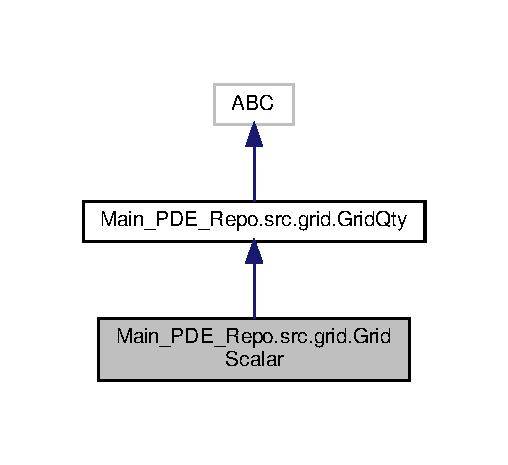
\includegraphics[width=244pt]{classMain__PDE__Repo_1_1src_1_1grid_1_1GridScalar__inherit__graph}
\end{center}
\end{figure}


Collaboration diagram for Main\+\_\+\+P\+D\+E\+\_\+\+Repo.\+src.\+grid.\+Grid\+Scalar\+:
\nopagebreak
\begin{figure}[H]
\begin{center}
\leavevmode
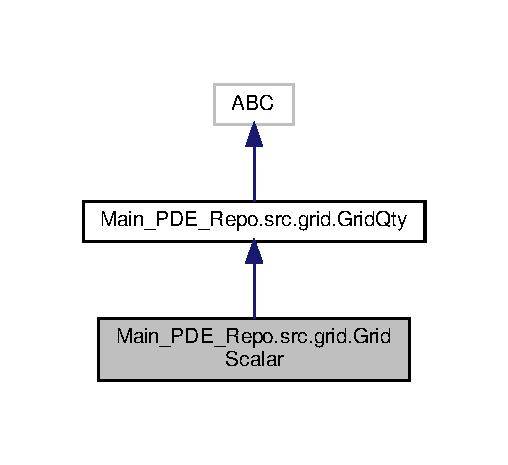
\includegraphics[width=244pt]{classMain__PDE__Repo_1_1src_1_1grid_1_1GridScalar__coll__graph}
\end{center}
\end{figure}
\subsection*{Public Member Functions}
\begin{DoxyCompactItemize}
\item 
def \hyperlink{classMain__PDE__Repo_1_1src_1_1grid_1_1GridScalar_ad7d2f2d7fade13d7e6f8d0eee5df0503}{\+\_\+\+\_\+add\+\_\+\+\_\+} (self, other)
\begin{DoxyCompactList}\small\item\em {\bfseries add} reformat magic method to add grids together element wise \end{DoxyCompactList}\item 
def \hyperlink{classMain__PDE__Repo_1_1src_1_1grid_1_1GridScalar_a8fb002038890b1ef82866d990ee76110}{\+\_\+\+\_\+radd\+\_\+\+\_\+} (self, other)
\item 
def \hyperlink{classMain__PDE__Repo_1_1src_1_1grid_1_1GridScalar_a2650dfa91626e64bee8a0788df81db88}{\+\_\+\+\_\+mul\+\_\+\+\_\+} (self, other)
\begin{DoxyCompactList}\small\item\em {\bfseries mul} reformat magic method of multiply to multiply two grids together elementwise \end{DoxyCompactList}\item 
def \hyperlink{classMain__PDE__Repo_1_1src_1_1grid_1_1GridScalar_ae4c09f385ca0bba688b4f6b0b6d9580d}{\+\_\+\+\_\+rmul\+\_\+\+\_\+} (self, other)
\item 
def \hyperlink{classMain__PDE__Repo_1_1src_1_1grid_1_1GridScalar_afbf5e11df0a675137c8bd157552f76e7}{apply\+Op} (self, opmat)
\end{DoxyCompactItemize}
\subsection*{Private Member Functions}
\begin{DoxyCompactItemize}
\item 
def \hyperlink{classMain__PDE__Repo_1_1src_1_1grid_1_1GridScalar_aa4fd978d7fa4c5344df660dfd296d2bf}{\+\_\+qtyshape} (self)
\item 
def \hyperlink{classMain__PDE__Repo_1_1src_1_1grid_1_1GridScalar_a9f5af1f06d9bf69fa130a77b64807bd4}{\+\_\+ravel} (self)
\begin{DoxyCompactList}\small\item\em \+\_\+ravel call np.\+ravel method on the underlying grid \end{DoxyCompactList}\end{DoxyCompactItemize}
\subsection*{Additional Inherited Members}


\subsection{Detailed Description}
the \hyperlink{classMain__PDE__Repo_1_1src_1_1grid_1_1GridScalar}{Grid\+Scalar} childclass 

\subsection{Member Function Documentation}
\mbox{\Hypertarget{classMain__PDE__Repo_1_1src_1_1grid_1_1GridScalar_ad7d2f2d7fade13d7e6f8d0eee5df0503}\label{classMain__PDE__Repo_1_1src_1_1grid_1_1GridScalar_ad7d2f2d7fade13d7e6f8d0eee5df0503}} 
\index{Main\+\_\+\+P\+D\+E\+\_\+\+Repo\+::src\+::grid\+::\+Grid\+Scalar@{Main\+\_\+\+P\+D\+E\+\_\+\+Repo\+::src\+::grid\+::\+Grid\+Scalar}!\+\_\+\+\_\+add\+\_\+\+\_\+@{\+\_\+\+\_\+add\+\_\+\+\_\+}}
\index{\+\_\+\+\_\+add\+\_\+\+\_\+@{\+\_\+\+\_\+add\+\_\+\+\_\+}!Main\+\_\+\+P\+D\+E\+\_\+\+Repo\+::src\+::grid\+::\+Grid\+Scalar@{Main\+\_\+\+P\+D\+E\+\_\+\+Repo\+::src\+::grid\+::\+Grid\+Scalar}}
\subsubsection{\texorpdfstring{\+\_\+\+\_\+add\+\_\+\+\_\+()}{\_\_add\_\_()}}
{\footnotesize\ttfamily def Main\+\_\+\+P\+D\+E\+\_\+\+Repo.\+src.\+grid.\+Grid\+Scalar.\+\_\+\+\_\+add\+\_\+\+\_\+ (\begin{DoxyParamCaption}\item[{}]{self,  }\item[{}]{other }\end{DoxyParamCaption})}



{\bfseries add} reformat magic method to add grids together element wise 

\mbox{\Hypertarget{classMain__PDE__Repo_1_1src_1_1grid_1_1GridScalar_a2650dfa91626e64bee8a0788df81db88}\label{classMain__PDE__Repo_1_1src_1_1grid_1_1GridScalar_a2650dfa91626e64bee8a0788df81db88}} 
\index{Main\+\_\+\+P\+D\+E\+\_\+\+Repo\+::src\+::grid\+::\+Grid\+Scalar@{Main\+\_\+\+P\+D\+E\+\_\+\+Repo\+::src\+::grid\+::\+Grid\+Scalar}!\+\_\+\+\_\+mul\+\_\+\+\_\+@{\+\_\+\+\_\+mul\+\_\+\+\_\+}}
\index{\+\_\+\+\_\+mul\+\_\+\+\_\+@{\+\_\+\+\_\+mul\+\_\+\+\_\+}!Main\+\_\+\+P\+D\+E\+\_\+\+Repo\+::src\+::grid\+::\+Grid\+Scalar@{Main\+\_\+\+P\+D\+E\+\_\+\+Repo\+::src\+::grid\+::\+Grid\+Scalar}}
\subsubsection{\texorpdfstring{\+\_\+\+\_\+mul\+\_\+\+\_\+()}{\_\_mul\_\_()}}
{\footnotesize\ttfamily def Main\+\_\+\+P\+D\+E\+\_\+\+Repo.\+src.\+grid.\+Grid\+Scalar.\+\_\+\+\_\+mul\+\_\+\+\_\+ (\begin{DoxyParamCaption}\item[{}]{self,  }\item[{}]{other }\end{DoxyParamCaption})}



{\bfseries mul} reformat magic method of multiply to multiply two grids together elementwise 

\mbox{\Hypertarget{classMain__PDE__Repo_1_1src_1_1grid_1_1GridScalar_a8fb002038890b1ef82866d990ee76110}\label{classMain__PDE__Repo_1_1src_1_1grid_1_1GridScalar_a8fb002038890b1ef82866d990ee76110}} 
\index{Main\+\_\+\+P\+D\+E\+\_\+\+Repo\+::src\+::grid\+::\+Grid\+Scalar@{Main\+\_\+\+P\+D\+E\+\_\+\+Repo\+::src\+::grid\+::\+Grid\+Scalar}!\+\_\+\+\_\+radd\+\_\+\+\_\+@{\+\_\+\+\_\+radd\+\_\+\+\_\+}}
\index{\+\_\+\+\_\+radd\+\_\+\+\_\+@{\+\_\+\+\_\+radd\+\_\+\+\_\+}!Main\+\_\+\+P\+D\+E\+\_\+\+Repo\+::src\+::grid\+::\+Grid\+Scalar@{Main\+\_\+\+P\+D\+E\+\_\+\+Repo\+::src\+::grid\+::\+Grid\+Scalar}}
\subsubsection{\texorpdfstring{\+\_\+\+\_\+radd\+\_\+\+\_\+()}{\_\_radd\_\_()}}
{\footnotesize\ttfamily def Main\+\_\+\+P\+D\+E\+\_\+\+Repo.\+src.\+grid.\+Grid\+Scalar.\+\_\+\+\_\+radd\+\_\+\+\_\+ (\begin{DoxyParamCaption}\item[{}]{self,  }\item[{}]{other }\end{DoxyParamCaption})}

\mbox{\Hypertarget{classMain__PDE__Repo_1_1src_1_1grid_1_1GridScalar_ae4c09f385ca0bba688b4f6b0b6d9580d}\label{classMain__PDE__Repo_1_1src_1_1grid_1_1GridScalar_ae4c09f385ca0bba688b4f6b0b6d9580d}} 
\index{Main\+\_\+\+P\+D\+E\+\_\+\+Repo\+::src\+::grid\+::\+Grid\+Scalar@{Main\+\_\+\+P\+D\+E\+\_\+\+Repo\+::src\+::grid\+::\+Grid\+Scalar}!\+\_\+\+\_\+rmul\+\_\+\+\_\+@{\+\_\+\+\_\+rmul\+\_\+\+\_\+}}
\index{\+\_\+\+\_\+rmul\+\_\+\+\_\+@{\+\_\+\+\_\+rmul\+\_\+\+\_\+}!Main\+\_\+\+P\+D\+E\+\_\+\+Repo\+::src\+::grid\+::\+Grid\+Scalar@{Main\+\_\+\+P\+D\+E\+\_\+\+Repo\+::src\+::grid\+::\+Grid\+Scalar}}
\subsubsection{\texorpdfstring{\+\_\+\+\_\+rmul\+\_\+\+\_\+()}{\_\_rmul\_\_()}}
{\footnotesize\ttfamily def Main\+\_\+\+P\+D\+E\+\_\+\+Repo.\+src.\+grid.\+Grid\+Scalar.\+\_\+\+\_\+rmul\+\_\+\+\_\+ (\begin{DoxyParamCaption}\item[{}]{self,  }\item[{}]{other }\end{DoxyParamCaption})}

\mbox{\Hypertarget{classMain__PDE__Repo_1_1src_1_1grid_1_1GridScalar_aa4fd978d7fa4c5344df660dfd296d2bf}\label{classMain__PDE__Repo_1_1src_1_1grid_1_1GridScalar_aa4fd978d7fa4c5344df660dfd296d2bf}} 
\index{Main\+\_\+\+P\+D\+E\+\_\+\+Repo\+::src\+::grid\+::\+Grid\+Scalar@{Main\+\_\+\+P\+D\+E\+\_\+\+Repo\+::src\+::grid\+::\+Grid\+Scalar}!\+\_\+qtyshape@{\+\_\+qtyshape}}
\index{\+\_\+qtyshape@{\+\_\+qtyshape}!Main\+\_\+\+P\+D\+E\+\_\+\+Repo\+::src\+::grid\+::\+Grid\+Scalar@{Main\+\_\+\+P\+D\+E\+\_\+\+Repo\+::src\+::grid\+::\+Grid\+Scalar}}
\subsubsection{\texorpdfstring{\+\_\+qtyshape()}{\_qtyshape()}}
{\footnotesize\ttfamily def Main\+\_\+\+P\+D\+E\+\_\+\+Repo.\+src.\+grid.\+Grid\+Scalar.\+\_\+qtyshape (\begin{DoxyParamCaption}\item[{}]{self }\end{DoxyParamCaption})\hspace{0.3cm}{\ttfamily [private]}}

\mbox{\Hypertarget{classMain__PDE__Repo_1_1src_1_1grid_1_1GridScalar_a9f5af1f06d9bf69fa130a77b64807bd4}\label{classMain__PDE__Repo_1_1src_1_1grid_1_1GridScalar_a9f5af1f06d9bf69fa130a77b64807bd4}} 
\index{Main\+\_\+\+P\+D\+E\+\_\+\+Repo\+::src\+::grid\+::\+Grid\+Scalar@{Main\+\_\+\+P\+D\+E\+\_\+\+Repo\+::src\+::grid\+::\+Grid\+Scalar}!\+\_\+ravel@{\+\_\+ravel}}
\index{\+\_\+ravel@{\+\_\+ravel}!Main\+\_\+\+P\+D\+E\+\_\+\+Repo\+::src\+::grid\+::\+Grid\+Scalar@{Main\+\_\+\+P\+D\+E\+\_\+\+Repo\+::src\+::grid\+::\+Grid\+Scalar}}
\subsubsection{\texorpdfstring{\+\_\+ravel()}{\_ravel()}}
{\footnotesize\ttfamily def Main\+\_\+\+P\+D\+E\+\_\+\+Repo.\+src.\+grid.\+Grid\+Scalar.\+\_\+ravel (\begin{DoxyParamCaption}\item[{}]{self }\end{DoxyParamCaption})\hspace{0.3cm}{\ttfamily [private]}}



\+\_\+ravel call np.\+ravel method on the underlying grid 

\mbox{\Hypertarget{classMain__PDE__Repo_1_1src_1_1grid_1_1GridScalar_afbf5e11df0a675137c8bd157552f76e7}\label{classMain__PDE__Repo_1_1src_1_1grid_1_1GridScalar_afbf5e11df0a675137c8bd157552f76e7}} 
\index{Main\+\_\+\+P\+D\+E\+\_\+\+Repo\+::src\+::grid\+::\+Grid\+Scalar@{Main\+\_\+\+P\+D\+E\+\_\+\+Repo\+::src\+::grid\+::\+Grid\+Scalar}!apply\+Op@{apply\+Op}}
\index{apply\+Op@{apply\+Op}!Main\+\_\+\+P\+D\+E\+\_\+\+Repo\+::src\+::grid\+::\+Grid\+Scalar@{Main\+\_\+\+P\+D\+E\+\_\+\+Repo\+::src\+::grid\+::\+Grid\+Scalar}}
\subsubsection{\texorpdfstring{apply\+Op()}{applyOp()}}
{\footnotesize\ttfamily def Main\+\_\+\+P\+D\+E\+\_\+\+Repo.\+src.\+grid.\+Grid\+Scalar.\+apply\+Op (\begin{DoxyParamCaption}\item[{}]{self,  }\item[{}]{opmat }\end{DoxyParamCaption})}



The documentation for this class was generated from the following file\+:\begin{DoxyCompactItemize}
\item 
src/\hyperlink{grid_8py}{grid.\+py}\end{DoxyCompactItemize}

\hypertarget{classMain__PDE__Repo_1_1src_1_1grid_1_1GridSpec}{}\section{Main\+\_\+\+P\+D\+E\+\_\+\+Repo.\+src.\+grid.\+Grid\+Spec Class Reference}
\label{classMain__PDE__Repo_1_1src_1_1grid_1_1GridSpec}\index{Main\+\_\+\+P\+D\+E\+\_\+\+Repo.\+src.\+grid.\+Grid\+Spec@{Main\+\_\+\+P\+D\+E\+\_\+\+Repo.\+src.\+grid.\+Grid\+Spec}}


the \hyperlink{classMain__PDE__Repo_1_1src_1_1grid_1_1GridSpec}{Grid\+Spec} abstract base class  




Inheritance diagram for Main\+\_\+\+P\+D\+E\+\_\+\+Repo.\+src.\+grid.\+Grid\+Spec\+:
\nopagebreak
\begin{figure}[H]
\begin{center}
\leavevmode
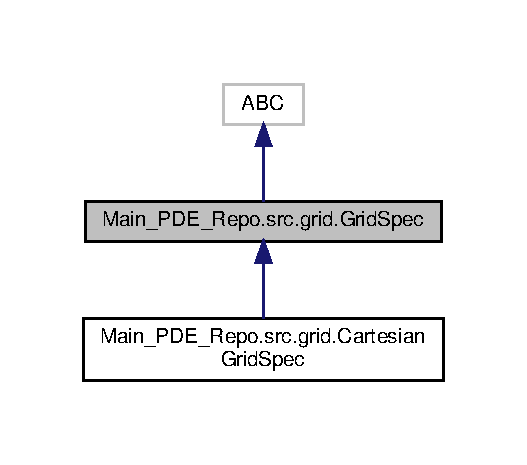
\includegraphics[width=253pt]{classMain__PDE__Repo_1_1src_1_1grid_1_1GridSpec__inherit__graph}
\end{center}
\end{figure}


Collaboration diagram for Main\+\_\+\+P\+D\+E\+\_\+\+Repo.\+src.\+grid.\+Grid\+Spec\+:
\nopagebreak
\begin{figure}[H]
\begin{center}
\leavevmode
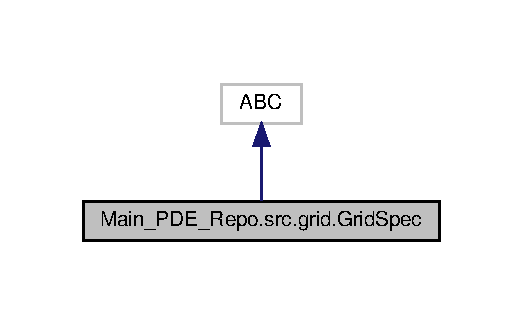
\includegraphics[width=251pt]{classMain__PDE__Repo_1_1src_1_1grid_1_1GridSpec__coll__graph}
\end{center}
\end{figure}


\subsection{Detailed Description}
the \hyperlink{classMain__PDE__Repo_1_1src_1_1grid_1_1GridSpec}{Grid\+Spec} abstract base class 

The documentation for this class was generated from the following file\+:\begin{DoxyCompactItemize}
\item 
src/\hyperlink{grid_8py}{grid.\+py}\end{DoxyCompactItemize}

\hypertarget{classMain__PDE__Repo_1_1src_1_1grid_1_1GridVector}{}\section{Main\+\_\+\+P\+D\+E\+\_\+\+Repo.\+src.\+grid.\+Grid\+Vector Class Reference}
\label{classMain__PDE__Repo_1_1src_1_1grid_1_1GridVector}\index{Main\+\_\+\+P\+D\+E\+\_\+\+Repo.\+src.\+grid.\+Grid\+Vector@{Main\+\_\+\+P\+D\+E\+\_\+\+Repo.\+src.\+grid.\+Grid\+Vector}}


the \hyperlink{classMain__PDE__Repo_1_1src_1_1grid_1_1GridVector}{Grid\+Vector} childclass  




Inheritance diagram for Main\+\_\+\+P\+D\+E\+\_\+\+Repo.\+src.\+grid.\+Grid\+Vector\+:
\nopagebreak
\begin{figure}[H]
\begin{center}
\leavevmode
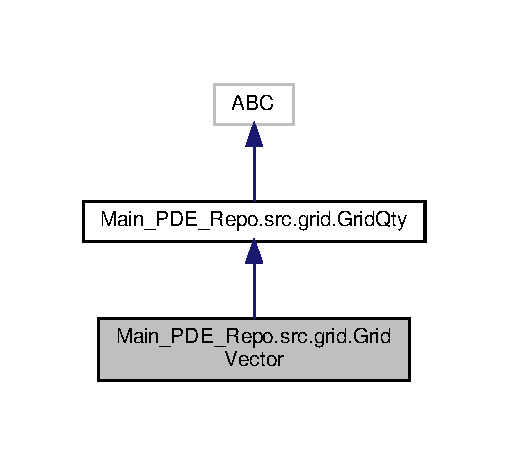
\includegraphics[width=244pt]{classMain__PDE__Repo_1_1src_1_1grid_1_1GridVector__inherit__graph}
\end{center}
\end{figure}


Collaboration diagram for Main\+\_\+\+P\+D\+E\+\_\+\+Repo.\+src.\+grid.\+Grid\+Vector\+:
\nopagebreak
\begin{figure}[H]
\begin{center}
\leavevmode
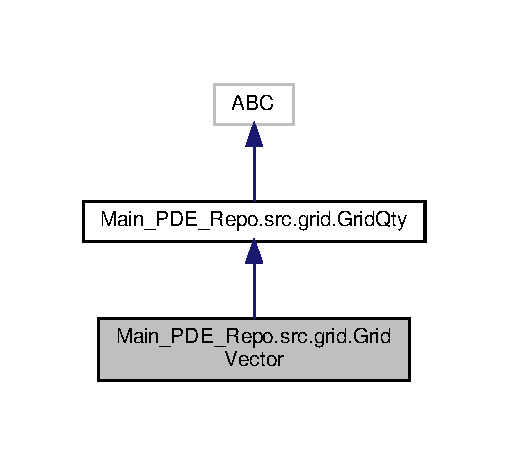
\includegraphics[width=244pt]{classMain__PDE__Repo_1_1src_1_1grid_1_1GridVector__coll__graph}
\end{center}
\end{figure}
\subsection*{Private Member Functions}
\begin{DoxyCompactItemize}
\item 
def \hyperlink{classMain__PDE__Repo_1_1src_1_1grid_1_1GridVector_ab622dfed79cd7bdf4c4049f7fb856e2b}{\+\_\+qtyshape} (self)
\end{DoxyCompactItemize}
\subsection*{Additional Inherited Members}


\subsection{Detailed Description}
the \hyperlink{classMain__PDE__Repo_1_1src_1_1grid_1_1GridVector}{Grid\+Vector} childclass 

\subsection{Member Function Documentation}
\mbox{\Hypertarget{classMain__PDE__Repo_1_1src_1_1grid_1_1GridVector_ab622dfed79cd7bdf4c4049f7fb856e2b}\label{classMain__PDE__Repo_1_1src_1_1grid_1_1GridVector_ab622dfed79cd7bdf4c4049f7fb856e2b}} 
\index{Main\+\_\+\+P\+D\+E\+\_\+\+Repo\+::src\+::grid\+::\+Grid\+Vector@{Main\+\_\+\+P\+D\+E\+\_\+\+Repo\+::src\+::grid\+::\+Grid\+Vector}!\+\_\+qtyshape@{\+\_\+qtyshape}}
\index{\+\_\+qtyshape@{\+\_\+qtyshape}!Main\+\_\+\+P\+D\+E\+\_\+\+Repo\+::src\+::grid\+::\+Grid\+Vector@{Main\+\_\+\+P\+D\+E\+\_\+\+Repo\+::src\+::grid\+::\+Grid\+Vector}}
\subsubsection{\texorpdfstring{\+\_\+qtyshape()}{\_qtyshape()}}
{\footnotesize\ttfamily def Main\+\_\+\+P\+D\+E\+\_\+\+Repo.\+src.\+grid.\+Grid\+Vector.\+\_\+qtyshape (\begin{DoxyParamCaption}\item[{}]{self }\end{DoxyParamCaption})\hspace{0.3cm}{\ttfamily [private]}}



The documentation for this class was generated from the following file\+:\begin{DoxyCompactItemize}
\item 
src/\hyperlink{grid_8py}{grid.\+py}\end{DoxyCompactItemize}

\hypertarget{classMain__PDE__Repo_1_1src_1_1logger_1_1Logger}{}\section{Main\+\_\+\+P\+D\+E\+\_\+\+Repo.\+src.\+logger.\+Logger Class Reference}
\label{classMain__PDE__Repo_1_1src_1_1logger_1_1Logger}\index{Main\+\_\+\+P\+D\+E\+\_\+\+Repo.\+src.\+logger.\+Logger@{Main\+\_\+\+P\+D\+E\+\_\+\+Repo.\+src.\+logger.\+Logger}}


The \hyperlink{classMain__PDE__Repo_1_1src_1_1logger_1_1Logger}{Logger} class.  


\subsection*{Public Member Functions}
\begin{DoxyCompactItemize}
\item 
def \hyperlink{classMain__PDE__Repo_1_1src_1_1logger_1_1Logger_a1cb1b576ea43629aba66f291b97099e2}{\+\_\+\+\_\+init\+\_\+\+\_\+} (self)
\begin{DoxyCompactList}\small\item\em The constructor initializes an empty list. \end{DoxyCompactList}\item 
def \hyperlink{classMain__PDE__Repo_1_1src_1_1logger_1_1Logger_a5028b1f1929f7124fc5322aaa917f118}{log} (self, t, val\+\_\+grid)
\begin{DoxyCompactList}\small\item\em The log function appends the current timestep. \end{DoxyCompactList}\item 
def \hyperlink{classMain__PDE__Repo_1_1src_1_1logger_1_1Logger_a07a3ec736e4a23eb8738f52fc0d27248}{get\+\_\+frame} (self, i)
\begin{DoxyCompactList}\small\item\em Function to get the log\+\_\+list element at a particular frame. \end{DoxyCompactList}\item 
def \hyperlink{classMain__PDE__Repo_1_1src_1_1logger_1_1Logger_a3a9c0a4d4efcc23c16de9f19652cb552}{get\+\_\+nframes} (self)
\begin{DoxyCompactList}\small\item\em Function to return the number of frame currently contained in the \hyperlink{classMain__PDE__Repo_1_1src_1_1logger_1_1Logger}{Logger} This is a wrapper of len(Logger\+Object.\+log\+\_\+list) in case we ever change how the log stores its stuff. \end{DoxyCompactList}\item 
def \hyperlink{classMain__PDE__Repo_1_1src_1_1logger_1_1Logger_af80ede43eb3e9305a18b9ede9f2a8607}{get\+\_\+data\+\_\+limits} (self)
\begin{DoxyCompactList}\small\item\em Function to get the min and max values of the data contained in the \hyperlink{classMain__PDE__Repo_1_1src_1_1logger_1_1Logger}{Logger}. \end{DoxyCompactList}\end{DoxyCompactItemize}
\subsection*{Public Attributes}
\begin{DoxyCompactItemize}
\item 
\hyperlink{classMain__PDE__Repo_1_1src_1_1logger_1_1Logger_a159655c83565fd1bfbbabb470ea7da0f}{log\+\_\+list}
\end{DoxyCompactItemize}


\subsection{Detailed Description}
The \hyperlink{classMain__PDE__Repo_1_1src_1_1logger_1_1Logger}{Logger} class. 

Basically a list wrapper. Just appends time and grid values to a list stored in the object. \hyperlink{classMain__PDE__Repo_1_1src_1_1logger_1_1Logger_a159655c83565fd1bfbbabb470ea7da0f}{Logger.\+log\+\_\+list}\mbox{[}index\mbox{]} returns the \mbox{[}t, val\+\_\+grid\mbox{]} pair at that index. 

\subsection{Constructor \& Destructor Documentation}
\mbox{\Hypertarget{classMain__PDE__Repo_1_1src_1_1logger_1_1Logger_a1cb1b576ea43629aba66f291b97099e2}\label{classMain__PDE__Repo_1_1src_1_1logger_1_1Logger_a1cb1b576ea43629aba66f291b97099e2}} 
\index{Main\+\_\+\+P\+D\+E\+\_\+\+Repo\+::src\+::logger\+::\+Logger@{Main\+\_\+\+P\+D\+E\+\_\+\+Repo\+::src\+::logger\+::\+Logger}!\+\_\+\+\_\+init\+\_\+\+\_\+@{\+\_\+\+\_\+init\+\_\+\+\_\+}}
\index{\+\_\+\+\_\+init\+\_\+\+\_\+@{\+\_\+\+\_\+init\+\_\+\+\_\+}!Main\+\_\+\+P\+D\+E\+\_\+\+Repo\+::src\+::logger\+::\+Logger@{Main\+\_\+\+P\+D\+E\+\_\+\+Repo\+::src\+::logger\+::\+Logger}}
\subsubsection{\texorpdfstring{\+\_\+\+\_\+init\+\_\+\+\_\+()}{\_\_init\_\_()}}
{\footnotesize\ttfamily def Main\+\_\+\+P\+D\+E\+\_\+\+Repo.\+src.\+logger.\+Logger.\+\_\+\+\_\+init\+\_\+\+\_\+ (\begin{DoxyParamCaption}\item[{}]{self }\end{DoxyParamCaption})}



The constructor initializes an empty list. 



\subsection{Member Function Documentation}
\mbox{\Hypertarget{classMain__PDE__Repo_1_1src_1_1logger_1_1Logger_af80ede43eb3e9305a18b9ede9f2a8607}\label{classMain__PDE__Repo_1_1src_1_1logger_1_1Logger_af80ede43eb3e9305a18b9ede9f2a8607}} 
\index{Main\+\_\+\+P\+D\+E\+\_\+\+Repo\+::src\+::logger\+::\+Logger@{Main\+\_\+\+P\+D\+E\+\_\+\+Repo\+::src\+::logger\+::\+Logger}!get\+\_\+data\+\_\+limits@{get\+\_\+data\+\_\+limits}}
\index{get\+\_\+data\+\_\+limits@{get\+\_\+data\+\_\+limits}!Main\+\_\+\+P\+D\+E\+\_\+\+Repo\+::src\+::logger\+::\+Logger@{Main\+\_\+\+P\+D\+E\+\_\+\+Repo\+::src\+::logger\+::\+Logger}}
\subsubsection{\texorpdfstring{get\+\_\+data\+\_\+limits()}{get\_data\_limits()}}
{\footnotesize\ttfamily def Main\+\_\+\+P\+D\+E\+\_\+\+Repo.\+src.\+logger.\+Logger.\+get\+\_\+data\+\_\+limits (\begin{DoxyParamCaption}\item[{}]{self }\end{DoxyParamCaption})}



Function to get the min and max values of the data contained in the \hyperlink{classMain__PDE__Repo_1_1src_1_1logger_1_1Logger}{Logger}. 

\mbox{\Hypertarget{classMain__PDE__Repo_1_1src_1_1logger_1_1Logger_a07a3ec736e4a23eb8738f52fc0d27248}\label{classMain__PDE__Repo_1_1src_1_1logger_1_1Logger_a07a3ec736e4a23eb8738f52fc0d27248}} 
\index{Main\+\_\+\+P\+D\+E\+\_\+\+Repo\+::src\+::logger\+::\+Logger@{Main\+\_\+\+P\+D\+E\+\_\+\+Repo\+::src\+::logger\+::\+Logger}!get\+\_\+frame@{get\+\_\+frame}}
\index{get\+\_\+frame@{get\+\_\+frame}!Main\+\_\+\+P\+D\+E\+\_\+\+Repo\+::src\+::logger\+::\+Logger@{Main\+\_\+\+P\+D\+E\+\_\+\+Repo\+::src\+::logger\+::\+Logger}}
\subsubsection{\texorpdfstring{get\+\_\+frame()}{get\_frame()}}
{\footnotesize\ttfamily def Main\+\_\+\+P\+D\+E\+\_\+\+Repo.\+src.\+logger.\+Logger.\+get\+\_\+frame (\begin{DoxyParamCaption}\item[{}]{self,  }\item[{}]{i }\end{DoxyParamCaption})}



Function to get the log\+\_\+list element at a particular frame. 


\begin{DoxyParams}{Parameters}
{\em i} & Int-\/ the frame that is desired, starting from 0 This is basically a wrapper of Logger\+Object.\+log\+\_\+list\mbox{[}i\mbox{]}, in case we ever want to change how the log stores its stuff. \\
\hline
\end{DoxyParams}
\mbox{\Hypertarget{classMain__PDE__Repo_1_1src_1_1logger_1_1Logger_a3a9c0a4d4efcc23c16de9f19652cb552}\label{classMain__PDE__Repo_1_1src_1_1logger_1_1Logger_a3a9c0a4d4efcc23c16de9f19652cb552}} 
\index{Main\+\_\+\+P\+D\+E\+\_\+\+Repo\+::src\+::logger\+::\+Logger@{Main\+\_\+\+P\+D\+E\+\_\+\+Repo\+::src\+::logger\+::\+Logger}!get\+\_\+nframes@{get\+\_\+nframes}}
\index{get\+\_\+nframes@{get\+\_\+nframes}!Main\+\_\+\+P\+D\+E\+\_\+\+Repo\+::src\+::logger\+::\+Logger@{Main\+\_\+\+P\+D\+E\+\_\+\+Repo\+::src\+::logger\+::\+Logger}}
\subsubsection{\texorpdfstring{get\+\_\+nframes()}{get\_nframes()}}
{\footnotesize\ttfamily def Main\+\_\+\+P\+D\+E\+\_\+\+Repo.\+src.\+logger.\+Logger.\+get\+\_\+nframes (\begin{DoxyParamCaption}\item[{}]{self }\end{DoxyParamCaption})}



Function to return the number of frame currently contained in the \hyperlink{classMain__PDE__Repo_1_1src_1_1logger_1_1Logger}{Logger} This is a wrapper of len(Logger\+Object.\+log\+\_\+list) in case we ever change how the log stores its stuff. 

\mbox{\Hypertarget{classMain__PDE__Repo_1_1src_1_1logger_1_1Logger_a5028b1f1929f7124fc5322aaa917f118}\label{classMain__PDE__Repo_1_1src_1_1logger_1_1Logger_a5028b1f1929f7124fc5322aaa917f118}} 
\index{Main\+\_\+\+P\+D\+E\+\_\+\+Repo\+::src\+::logger\+::\+Logger@{Main\+\_\+\+P\+D\+E\+\_\+\+Repo\+::src\+::logger\+::\+Logger}!log@{log}}
\index{log@{log}!Main\+\_\+\+P\+D\+E\+\_\+\+Repo\+::src\+::logger\+::\+Logger@{Main\+\_\+\+P\+D\+E\+\_\+\+Repo\+::src\+::logger\+::\+Logger}}
\subsubsection{\texorpdfstring{log()}{log()}}
{\footnotesize\ttfamily def Main\+\_\+\+P\+D\+E\+\_\+\+Repo.\+src.\+logger.\+Logger.\+log (\begin{DoxyParamCaption}\item[{}]{self,  }\item[{}]{t,  }\item[{}]{val\+\_\+grid }\end{DoxyParamCaption})}



The log function appends the current timestep. 


\begin{DoxyParams}{Parameters}
{\em t} & The current time value \\
\hline
{\em val\+\_\+grid} & The current spatial grid values to be logged \\
\hline
\end{DoxyParams}


\subsection{Member Data Documentation}
\mbox{\Hypertarget{classMain__PDE__Repo_1_1src_1_1logger_1_1Logger_a159655c83565fd1bfbbabb470ea7da0f}\label{classMain__PDE__Repo_1_1src_1_1logger_1_1Logger_a159655c83565fd1bfbbabb470ea7da0f}} 
\index{Main\+\_\+\+P\+D\+E\+\_\+\+Repo\+::src\+::logger\+::\+Logger@{Main\+\_\+\+P\+D\+E\+\_\+\+Repo\+::src\+::logger\+::\+Logger}!log\+\_\+list@{log\+\_\+list}}
\index{log\+\_\+list@{log\+\_\+list}!Main\+\_\+\+P\+D\+E\+\_\+\+Repo\+::src\+::logger\+::\+Logger@{Main\+\_\+\+P\+D\+E\+\_\+\+Repo\+::src\+::logger\+::\+Logger}}
\subsubsection{\texorpdfstring{log\+\_\+list}{log\_list}}
{\footnotesize\ttfamily Main\+\_\+\+P\+D\+E\+\_\+\+Repo.\+src.\+logger.\+Logger.\+log\+\_\+list}



The documentation for this class was generated from the following file\+:\begin{DoxyCompactItemize}
\item 
src/\hyperlink{logger_8py}{logger.\+py}\end{DoxyCompactItemize}

\hypertarget{classMain__PDE__Repo_1_1src_1_1mesh_1_1Mesh}{}\section{Main\+\_\+\+P\+D\+E\+\_\+\+Repo.\+src.\+mesh.\+Mesh Class Reference}
\label{classMain__PDE__Repo_1_1src_1_1mesh_1_1Mesh}\index{Main\+\_\+\+P\+D\+E\+\_\+\+Repo.\+src.\+mesh.\+Mesh@{Main\+\_\+\+P\+D\+E\+\_\+\+Repo.\+src.\+mesh.\+Mesh}}


\hyperlink{classMain__PDE__Repo_1_1src_1_1mesh_1_1Mesh}{Mesh} A set of arrays generated from a base grid containing key value paris stored in matricies.  


\subsection*{Public Member Functions}
\begin{DoxyCompactItemize}
\item 
def \hyperlink{classMain__PDE__Repo_1_1src_1_1mesh_1_1Mesh_a6b6acfdda769157a8d3b762b8e60106e}{\+\_\+\+\_\+init\+\_\+\+\_\+} (self, \hyperlink{classMain__PDE__Repo_1_1src_1_1mesh_1_1Mesh_a6f83620aa1c76185e2b81412957a4758}{shape})
\item 
def \hyperlink{classMain__PDE__Repo_1_1src_1_1mesh_1_1Mesh_ab5af22f5310645d40c4ce2e420b1b21e}{\+\_\+\+\_\+getitem\+\_\+\+\_\+} (self, key)
\begin{DoxyCompactList}\small\item\em {\bfseries getitem} Overwrite getitem method to return a tuple of values corresponding the the relevant item in each dimesnion\textquotesingle{}s mesh \end{DoxyCompactList}\item 
def \hyperlink{classMain__PDE__Repo_1_1src_1_1mesh_1_1Mesh_a6f83620aa1c76185e2b81412957a4758}{shape} (self)
\begin{DoxyCompactList}\small\item\em shape Return the shape of the mesh \end{DoxyCompactList}\item 
def \hyperlink{classMain__PDE__Repo_1_1src_1_1mesh_1_1Mesh_afcb5da499b85e096c5ab20bbf11ad1c6}{slice} (self, slices)
\begin{DoxyCompactList}\small\item\em slice Slice each mesh according to a given set of slices \end{DoxyCompactList}\item 
def \hyperlink{classMain__PDE__Repo_1_1src_1_1mesh_1_1Mesh_adfbc08946443424b523a771ca67a7009}{sub\+\_\+slice} (self, slices)
\begin{DoxyCompactList}\small\item\em subslice generate a new mesh object corresponding to the original mesh object sliced along the relevant slices \end{DoxyCompactList}\end{DoxyCompactItemize}
\subsection*{Public Attributes}
\begin{DoxyCompactItemize}
\item 
\hyperlink{classMain__PDE__Repo_1_1src_1_1mesh_1_1Mesh_a1da23a0977d75b18603c49d2c7bf59ba}{base\+\_\+shape}
\item 
\hyperlink{classMain__PDE__Repo_1_1src_1_1mesh_1_1Mesh_a3b4d75bfb8cf60c362ab018eb26202ba}{dim}
\item 
\hyperlink{classMain__PDE__Repo_1_1src_1_1mesh_1_1Mesh_aa2e44de653f55fa440bde47a47fc67f0}{meshes}
\end{DoxyCompactItemize}
\subsection*{Private Member Functions}
\begin{DoxyCompactItemize}
\item 
def \hyperlink{classMain__PDE__Repo_1_1src_1_1mesh_1_1Mesh_a9229b4fc718a95c8f6b0fe47d6a16867}{\+\_\+gen\+\_\+grid} (self)
\end{DoxyCompactItemize}


\subsection{Detailed Description}
\hyperlink{classMain__PDE__Repo_1_1src_1_1mesh_1_1Mesh}{Mesh} A set of arrays generated from a base grid containing key value paris stored in matricies. 

Generates a gridmesh for a given shape of base grid and then stores that as an n-\/dimensional tuple where n is the dimension of the base grid 

\subsection{Constructor \& Destructor Documentation}
\mbox{\Hypertarget{classMain__PDE__Repo_1_1src_1_1mesh_1_1Mesh_a6b6acfdda769157a8d3b762b8e60106e}\label{classMain__PDE__Repo_1_1src_1_1mesh_1_1Mesh_a6b6acfdda769157a8d3b762b8e60106e}} 
\index{Main\+\_\+\+P\+D\+E\+\_\+\+Repo\+::src\+::mesh\+::\+Mesh@{Main\+\_\+\+P\+D\+E\+\_\+\+Repo\+::src\+::mesh\+::\+Mesh}!\+\_\+\+\_\+init\+\_\+\+\_\+@{\+\_\+\+\_\+init\+\_\+\+\_\+}}
\index{\+\_\+\+\_\+init\+\_\+\+\_\+@{\+\_\+\+\_\+init\+\_\+\+\_\+}!Main\+\_\+\+P\+D\+E\+\_\+\+Repo\+::src\+::mesh\+::\+Mesh@{Main\+\_\+\+P\+D\+E\+\_\+\+Repo\+::src\+::mesh\+::\+Mesh}}
\subsubsection{\texorpdfstring{\+\_\+\+\_\+init\+\_\+\+\_\+()}{\_\_init\_\_()}}
{\footnotesize\ttfamily def Main\+\_\+\+P\+D\+E\+\_\+\+Repo.\+src.\+mesh.\+Mesh.\+\_\+\+\_\+init\+\_\+\+\_\+ (\begin{DoxyParamCaption}\item[{}]{self,  }\item[{}]{shape }\end{DoxyParamCaption})}



\subsection{Member Function Documentation}
\mbox{\Hypertarget{classMain__PDE__Repo_1_1src_1_1mesh_1_1Mesh_ab5af22f5310645d40c4ce2e420b1b21e}\label{classMain__PDE__Repo_1_1src_1_1mesh_1_1Mesh_ab5af22f5310645d40c4ce2e420b1b21e}} 
\index{Main\+\_\+\+P\+D\+E\+\_\+\+Repo\+::src\+::mesh\+::\+Mesh@{Main\+\_\+\+P\+D\+E\+\_\+\+Repo\+::src\+::mesh\+::\+Mesh}!\+\_\+\+\_\+getitem\+\_\+\+\_\+@{\+\_\+\+\_\+getitem\+\_\+\+\_\+}}
\index{\+\_\+\+\_\+getitem\+\_\+\+\_\+@{\+\_\+\+\_\+getitem\+\_\+\+\_\+}!Main\+\_\+\+P\+D\+E\+\_\+\+Repo\+::src\+::mesh\+::\+Mesh@{Main\+\_\+\+P\+D\+E\+\_\+\+Repo\+::src\+::mesh\+::\+Mesh}}
\subsubsection{\texorpdfstring{\+\_\+\+\_\+getitem\+\_\+\+\_\+()}{\_\_getitem\_\_()}}
{\footnotesize\ttfamily def Main\+\_\+\+P\+D\+E\+\_\+\+Repo.\+src.\+mesh.\+Mesh.\+\_\+\+\_\+getitem\+\_\+\+\_\+ (\begin{DoxyParamCaption}\item[{}]{self,  }\item[{}]{key }\end{DoxyParamCaption})}



{\bfseries getitem} Overwrite getitem method to return a tuple of values corresponding the the relevant item in each dimesnion\textquotesingle{}s mesh 

\mbox{\Hypertarget{classMain__PDE__Repo_1_1src_1_1mesh_1_1Mesh_a9229b4fc718a95c8f6b0fe47d6a16867}\label{classMain__PDE__Repo_1_1src_1_1mesh_1_1Mesh_a9229b4fc718a95c8f6b0fe47d6a16867}} 
\index{Main\+\_\+\+P\+D\+E\+\_\+\+Repo\+::src\+::mesh\+::\+Mesh@{Main\+\_\+\+P\+D\+E\+\_\+\+Repo\+::src\+::mesh\+::\+Mesh}!\+\_\+gen\+\_\+grid@{\+\_\+gen\+\_\+grid}}
\index{\+\_\+gen\+\_\+grid@{\+\_\+gen\+\_\+grid}!Main\+\_\+\+P\+D\+E\+\_\+\+Repo\+::src\+::mesh\+::\+Mesh@{Main\+\_\+\+P\+D\+E\+\_\+\+Repo\+::src\+::mesh\+::\+Mesh}}
\subsubsection{\texorpdfstring{\+\_\+gen\+\_\+grid()}{\_gen\_grid()}}
{\footnotesize\ttfamily def Main\+\_\+\+P\+D\+E\+\_\+\+Repo.\+src.\+mesh.\+Mesh.\+\_\+gen\+\_\+grid (\begin{DoxyParamCaption}\item[{}]{self }\end{DoxyParamCaption})\hspace{0.3cm}{\ttfamily [private]}}

\mbox{\Hypertarget{classMain__PDE__Repo_1_1src_1_1mesh_1_1Mesh_a6f83620aa1c76185e2b81412957a4758}\label{classMain__PDE__Repo_1_1src_1_1mesh_1_1Mesh_a6f83620aa1c76185e2b81412957a4758}} 
\index{Main\+\_\+\+P\+D\+E\+\_\+\+Repo\+::src\+::mesh\+::\+Mesh@{Main\+\_\+\+P\+D\+E\+\_\+\+Repo\+::src\+::mesh\+::\+Mesh}!shape@{shape}}
\index{shape@{shape}!Main\+\_\+\+P\+D\+E\+\_\+\+Repo\+::src\+::mesh\+::\+Mesh@{Main\+\_\+\+P\+D\+E\+\_\+\+Repo\+::src\+::mesh\+::\+Mesh}}
\subsubsection{\texorpdfstring{shape()}{shape()}}
{\footnotesize\ttfamily def Main\+\_\+\+P\+D\+E\+\_\+\+Repo.\+src.\+mesh.\+Mesh.\+shape (\begin{DoxyParamCaption}\item[{}]{self }\end{DoxyParamCaption})}



shape Return the shape of the mesh 

\mbox{\Hypertarget{classMain__PDE__Repo_1_1src_1_1mesh_1_1Mesh_afcb5da499b85e096c5ab20bbf11ad1c6}\label{classMain__PDE__Repo_1_1src_1_1mesh_1_1Mesh_afcb5da499b85e096c5ab20bbf11ad1c6}} 
\index{Main\+\_\+\+P\+D\+E\+\_\+\+Repo\+::src\+::mesh\+::\+Mesh@{Main\+\_\+\+P\+D\+E\+\_\+\+Repo\+::src\+::mesh\+::\+Mesh}!slice@{slice}}
\index{slice@{slice}!Main\+\_\+\+P\+D\+E\+\_\+\+Repo\+::src\+::mesh\+::\+Mesh@{Main\+\_\+\+P\+D\+E\+\_\+\+Repo\+::src\+::mesh\+::\+Mesh}}
\subsubsection{\texorpdfstring{slice()}{slice()}}
{\footnotesize\ttfamily def Main\+\_\+\+P\+D\+E\+\_\+\+Repo.\+src.\+mesh.\+Mesh.\+slice (\begin{DoxyParamCaption}\item[{}]{self,  }\item[{}]{slices }\end{DoxyParamCaption})}



slice Slice each mesh according to a given set of slices 

Takes a set of slices for each dimension of the mesh and performs the appropriate subslicing for each dimension\textquotesingle{}s grid and returns the subslices as a tuple 
\begin{DoxyParams}{Parameters}
{\em slices} & tuple of tuples corresponding to the start and end index wanted in each underlying dimension \\
\hline
\end{DoxyParams}
\mbox{\Hypertarget{classMain__PDE__Repo_1_1src_1_1mesh_1_1Mesh_adfbc08946443424b523a771ca67a7009}\label{classMain__PDE__Repo_1_1src_1_1mesh_1_1Mesh_adfbc08946443424b523a771ca67a7009}} 
\index{Main\+\_\+\+P\+D\+E\+\_\+\+Repo\+::src\+::mesh\+::\+Mesh@{Main\+\_\+\+P\+D\+E\+\_\+\+Repo\+::src\+::mesh\+::\+Mesh}!sub\+\_\+slice@{sub\+\_\+slice}}
\index{sub\+\_\+slice@{sub\+\_\+slice}!Main\+\_\+\+P\+D\+E\+\_\+\+Repo\+::src\+::mesh\+::\+Mesh@{Main\+\_\+\+P\+D\+E\+\_\+\+Repo\+::src\+::mesh\+::\+Mesh}}
\subsubsection{\texorpdfstring{sub\+\_\+slice()}{sub\_slice()}}
{\footnotesize\ttfamily def Main\+\_\+\+P\+D\+E\+\_\+\+Repo.\+src.\+mesh.\+Mesh.\+sub\+\_\+slice (\begin{DoxyParamCaption}\item[{}]{self,  }\item[{}]{slices }\end{DoxyParamCaption})}



subslice generate a new mesh object corresponding to the original mesh object sliced along the relevant slices 


\begin{DoxyParams}{Parameters}
{\em slices} & tuple of tuples corresponding to the start and end index wanted in each underlying dimension \\
\hline
\end{DoxyParams}


\subsection{Member Data Documentation}
\mbox{\Hypertarget{classMain__PDE__Repo_1_1src_1_1mesh_1_1Mesh_a1da23a0977d75b18603c49d2c7bf59ba}\label{classMain__PDE__Repo_1_1src_1_1mesh_1_1Mesh_a1da23a0977d75b18603c49d2c7bf59ba}} 
\index{Main\+\_\+\+P\+D\+E\+\_\+\+Repo\+::src\+::mesh\+::\+Mesh@{Main\+\_\+\+P\+D\+E\+\_\+\+Repo\+::src\+::mesh\+::\+Mesh}!base\+\_\+shape@{base\+\_\+shape}}
\index{base\+\_\+shape@{base\+\_\+shape}!Main\+\_\+\+P\+D\+E\+\_\+\+Repo\+::src\+::mesh\+::\+Mesh@{Main\+\_\+\+P\+D\+E\+\_\+\+Repo\+::src\+::mesh\+::\+Mesh}}
\subsubsection{\texorpdfstring{base\+\_\+shape}{base\_shape}}
{\footnotesize\ttfamily Main\+\_\+\+P\+D\+E\+\_\+\+Repo.\+src.\+mesh.\+Mesh.\+base\+\_\+shape}

\mbox{\Hypertarget{classMain__PDE__Repo_1_1src_1_1mesh_1_1Mesh_a3b4d75bfb8cf60c362ab018eb26202ba}\label{classMain__PDE__Repo_1_1src_1_1mesh_1_1Mesh_a3b4d75bfb8cf60c362ab018eb26202ba}} 
\index{Main\+\_\+\+P\+D\+E\+\_\+\+Repo\+::src\+::mesh\+::\+Mesh@{Main\+\_\+\+P\+D\+E\+\_\+\+Repo\+::src\+::mesh\+::\+Mesh}!dim@{dim}}
\index{dim@{dim}!Main\+\_\+\+P\+D\+E\+\_\+\+Repo\+::src\+::mesh\+::\+Mesh@{Main\+\_\+\+P\+D\+E\+\_\+\+Repo\+::src\+::mesh\+::\+Mesh}}
\subsubsection{\texorpdfstring{dim}{dim}}
{\footnotesize\ttfamily Main\+\_\+\+P\+D\+E\+\_\+\+Repo.\+src.\+mesh.\+Mesh.\+dim}

\mbox{\Hypertarget{classMain__PDE__Repo_1_1src_1_1mesh_1_1Mesh_aa2e44de653f55fa440bde47a47fc67f0}\label{classMain__PDE__Repo_1_1src_1_1mesh_1_1Mesh_aa2e44de653f55fa440bde47a47fc67f0}} 
\index{Main\+\_\+\+P\+D\+E\+\_\+\+Repo\+::src\+::mesh\+::\+Mesh@{Main\+\_\+\+P\+D\+E\+\_\+\+Repo\+::src\+::mesh\+::\+Mesh}!meshes@{meshes}}
\index{meshes@{meshes}!Main\+\_\+\+P\+D\+E\+\_\+\+Repo\+::src\+::mesh\+::\+Mesh@{Main\+\_\+\+P\+D\+E\+\_\+\+Repo\+::src\+::mesh\+::\+Mesh}}
\subsubsection{\texorpdfstring{meshes}{meshes}}
{\footnotesize\ttfamily Main\+\_\+\+P\+D\+E\+\_\+\+Repo.\+src.\+mesh.\+Mesh.\+meshes}



The documentation for this class was generated from the following file\+:\begin{DoxyCompactItemize}
\item 
src/\hyperlink{mesh_8py}{mesh.\+py}\end{DoxyCompactItemize}

\hypertarget{classMain__PDE__Repo_1_1src_1_1static__bcs_1_1Neumann}{}\section{Main\+\_\+\+P\+D\+E\+\_\+\+Repo.\+src.\+static\+\_\+bcs.\+Neumann Class Reference}
\label{classMain__PDE__Repo_1_1src_1_1static__bcs_1_1Neumann}\index{Main\+\_\+\+P\+D\+E\+\_\+\+Repo.\+src.\+static\+\_\+bcs.\+Neumann@{Main\+\_\+\+P\+D\+E\+\_\+\+Repo.\+src.\+static\+\_\+bcs.\+Neumann}}


Child \hyperlink{namespaceMain__PDE__Repo_1_1src_1_1BCs}{B\+Cs} class for handling one side with static \hyperlink{classMain__PDE__Repo_1_1src_1_1static__bcs_1_1Neumann}{Neumann} boundary conditions.  




Inheritance diagram for Main\+\_\+\+P\+D\+E\+\_\+\+Repo.\+src.\+static\+\_\+bcs.\+Neumann\+:
\nopagebreak
\begin{figure}[H]
\begin{center}
\leavevmode
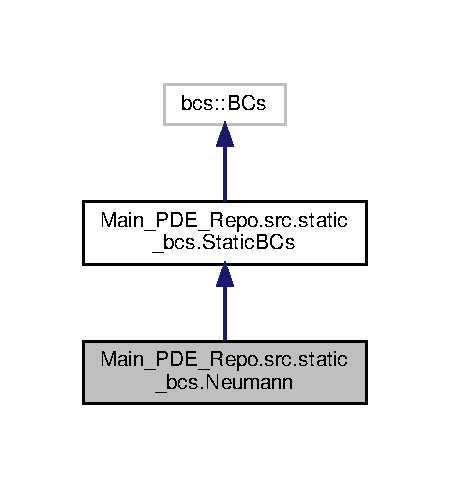
\includegraphics[width=216pt]{classMain__PDE__Repo_1_1src_1_1static__bcs_1_1Neumann__inherit__graph}
\end{center}
\end{figure}


Collaboration diagram for Main\+\_\+\+P\+D\+E\+\_\+\+Repo.\+src.\+static\+\_\+bcs.\+Neumann\+:
\nopagebreak
\begin{figure}[H]
\begin{center}
\leavevmode
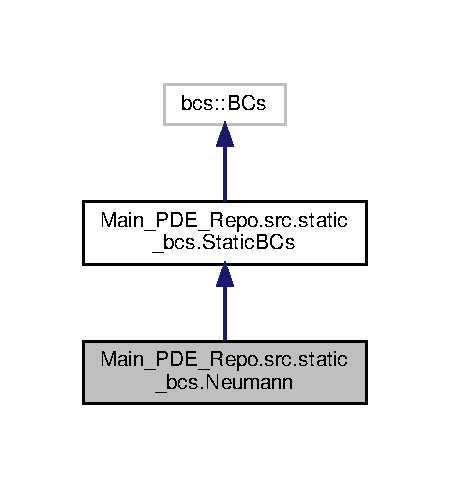
\includegraphics[width=216pt]{classMain__PDE__Repo_1_1src_1_1static__bcs_1_1Neumann__coll__graph}
\end{center}
\end{figure}
\subsection*{Additional Inherited Members}


\subsection{Detailed Description}
Child \hyperlink{namespaceMain__PDE__Repo_1_1src_1_1BCs}{B\+Cs} class for handling one side with static \hyperlink{classMain__PDE__Repo_1_1src_1_1static__bcs_1_1Neumann}{Neumann} boundary conditions. 



The documentation for this class was generated from the following file\+:\begin{DoxyCompactItemize}
\item 
src/\hyperlink{static__bcs_8py}{static\+\_\+bcs.\+py}\end{DoxyCompactItemize}

\hypertarget{classMain__PDE__Repo_1_1src_1_1operator__1d_1_1Operator1D}{}\section{Main\+\_\+\+P\+D\+E\+\_\+\+Repo.\+src.\+operator\+\_\+1d.\+Operator1D Class Reference}
\label{classMain__PDE__Repo_1_1src_1_1operator__1d_1_1Operator1D}\index{Main\+\_\+\+P\+D\+E\+\_\+\+Repo.\+src.\+operator\+\_\+1d.\+Operator1D@{Main\+\_\+\+P\+D\+E\+\_\+\+Repo.\+src.\+operator\+\_\+1d.\+Operator1D}}


The \hyperlink{classMain__PDE__Repo_1_1src_1_1operator__1d_1_1Operator1D}{Operator1D} class.  


\subsection*{Public Member Functions}
\begin{DoxyCompactItemize}
\item 
def \hyperlink{classMain__PDE__Repo_1_1src_1_1operator__1d_1_1Operator1D_a4e18976c3de7791d78f8a8950ec50d2f}{\+\_\+\+\_\+init\+\_\+\+\_\+} (self, s\+\_\+list, \hyperlink{classMain__PDE__Repo_1_1src_1_1operator__1d_1_1Operator1D_a84edadfc5eadaa3c21e56c51cbe9c94b}{deg})
\begin{DoxyCompactList}\small\item\em 1D Operator constructor \end{DoxyCompactList}\end{DoxyCompactItemize}
\subsection*{Public Attributes}
\begin{DoxyCompactItemize}
\item 
\hyperlink{classMain__PDE__Repo_1_1src_1_1operator__1d_1_1Operator1D_a37a9116a49b9aa2a799a7a6afe93b2cb}{stncl}
\item 
\hyperlink{classMain__PDE__Repo_1_1src_1_1operator__1d_1_1Operator1D_a84edadfc5eadaa3c21e56c51cbe9c94b}{deg}
\item 
\hyperlink{classMain__PDE__Repo_1_1src_1_1operator__1d_1_1Operator1D_a1b236addd7ef51377c7de08475afc2a8}{accuracy}
\item 
\hyperlink{classMain__PDE__Repo_1_1src_1_1operator__1d_1_1Operator1D_a5c14bf1f562fbd76aa191a37e1ca8355}{weights}
\end{DoxyCompactItemize}


\subsection{Detailed Description}
The \hyperlink{classMain__PDE__Repo_1_1src_1_1operator__1d_1_1Operator1D}{Operator1D} class. 

\subsection{Constructor \& Destructor Documentation}
\mbox{\Hypertarget{classMain__PDE__Repo_1_1src_1_1operator__1d_1_1Operator1D_a4e18976c3de7791d78f8a8950ec50d2f}\label{classMain__PDE__Repo_1_1src_1_1operator__1d_1_1Operator1D_a4e18976c3de7791d78f8a8950ec50d2f}} 
\index{Main\+\_\+\+P\+D\+E\+\_\+\+Repo\+::src\+::operator\+\_\+1d\+::\+Operator1D@{Main\+\_\+\+P\+D\+E\+\_\+\+Repo\+::src\+::operator\+\_\+1d\+::\+Operator1D}!\+\_\+\+\_\+init\+\_\+\+\_\+@{\+\_\+\+\_\+init\+\_\+\+\_\+}}
\index{\+\_\+\+\_\+init\+\_\+\+\_\+@{\+\_\+\+\_\+init\+\_\+\+\_\+}!Main\+\_\+\+P\+D\+E\+\_\+\+Repo\+::src\+::operator\+\_\+1d\+::\+Operator1D@{Main\+\_\+\+P\+D\+E\+\_\+\+Repo\+::src\+::operator\+\_\+1d\+::\+Operator1D}}
\subsubsection{\texorpdfstring{\+\_\+\+\_\+init\+\_\+\+\_\+()}{\_\_init\_\_()}}
{\footnotesize\ttfamily def Main\+\_\+\+P\+D\+E\+\_\+\+Repo.\+src.\+operator\+\_\+1d.\+Operator1\+D.\+\_\+\+\_\+init\+\_\+\+\_\+ (\begin{DoxyParamCaption}\item[{}]{self,  }\item[{}]{s\+\_\+list,  }\item[{}]{deg }\end{DoxyParamCaption})}



1D Operator constructor 


\begin{DoxyParams}{Parameters}
{\em s\+\_\+list} & A list of stencil index points \\
\hline
{\em deg} & The degree of the desired derivative \\
\hline
\end{DoxyParams}


\subsection{Member Data Documentation}
\mbox{\Hypertarget{classMain__PDE__Repo_1_1src_1_1operator__1d_1_1Operator1D_a1b236addd7ef51377c7de08475afc2a8}\label{classMain__PDE__Repo_1_1src_1_1operator__1d_1_1Operator1D_a1b236addd7ef51377c7de08475afc2a8}} 
\index{Main\+\_\+\+P\+D\+E\+\_\+\+Repo\+::src\+::operator\+\_\+1d\+::\+Operator1D@{Main\+\_\+\+P\+D\+E\+\_\+\+Repo\+::src\+::operator\+\_\+1d\+::\+Operator1D}!accuracy@{accuracy}}
\index{accuracy@{accuracy}!Main\+\_\+\+P\+D\+E\+\_\+\+Repo\+::src\+::operator\+\_\+1d\+::\+Operator1D@{Main\+\_\+\+P\+D\+E\+\_\+\+Repo\+::src\+::operator\+\_\+1d\+::\+Operator1D}}
\subsubsection{\texorpdfstring{accuracy}{accuracy}}
{\footnotesize\ttfamily Main\+\_\+\+P\+D\+E\+\_\+\+Repo.\+src.\+operator\+\_\+1d.\+Operator1\+D.\+accuracy}

\mbox{\Hypertarget{classMain__PDE__Repo_1_1src_1_1operator__1d_1_1Operator1D_a84edadfc5eadaa3c21e56c51cbe9c94b}\label{classMain__PDE__Repo_1_1src_1_1operator__1d_1_1Operator1D_a84edadfc5eadaa3c21e56c51cbe9c94b}} 
\index{Main\+\_\+\+P\+D\+E\+\_\+\+Repo\+::src\+::operator\+\_\+1d\+::\+Operator1D@{Main\+\_\+\+P\+D\+E\+\_\+\+Repo\+::src\+::operator\+\_\+1d\+::\+Operator1D}!deg@{deg}}
\index{deg@{deg}!Main\+\_\+\+P\+D\+E\+\_\+\+Repo\+::src\+::operator\+\_\+1d\+::\+Operator1D@{Main\+\_\+\+P\+D\+E\+\_\+\+Repo\+::src\+::operator\+\_\+1d\+::\+Operator1D}}
\subsubsection{\texorpdfstring{deg}{deg}}
{\footnotesize\ttfamily Main\+\_\+\+P\+D\+E\+\_\+\+Repo.\+src.\+operator\+\_\+1d.\+Operator1\+D.\+deg}

\mbox{\Hypertarget{classMain__PDE__Repo_1_1src_1_1operator__1d_1_1Operator1D_a37a9116a49b9aa2a799a7a6afe93b2cb}\label{classMain__PDE__Repo_1_1src_1_1operator__1d_1_1Operator1D_a37a9116a49b9aa2a799a7a6afe93b2cb}} 
\index{Main\+\_\+\+P\+D\+E\+\_\+\+Repo\+::src\+::operator\+\_\+1d\+::\+Operator1D@{Main\+\_\+\+P\+D\+E\+\_\+\+Repo\+::src\+::operator\+\_\+1d\+::\+Operator1D}!stncl@{stncl}}
\index{stncl@{stncl}!Main\+\_\+\+P\+D\+E\+\_\+\+Repo\+::src\+::operator\+\_\+1d\+::\+Operator1D@{Main\+\_\+\+P\+D\+E\+\_\+\+Repo\+::src\+::operator\+\_\+1d\+::\+Operator1D}}
\subsubsection{\texorpdfstring{stncl}{stncl}}
{\footnotesize\ttfamily Main\+\_\+\+P\+D\+E\+\_\+\+Repo.\+src.\+operator\+\_\+1d.\+Operator1\+D.\+stncl}

\mbox{\Hypertarget{classMain__PDE__Repo_1_1src_1_1operator__1d_1_1Operator1D_a5c14bf1f562fbd76aa191a37e1ca8355}\label{classMain__PDE__Repo_1_1src_1_1operator__1d_1_1Operator1D_a5c14bf1f562fbd76aa191a37e1ca8355}} 
\index{Main\+\_\+\+P\+D\+E\+\_\+\+Repo\+::src\+::operator\+\_\+1d\+::\+Operator1D@{Main\+\_\+\+P\+D\+E\+\_\+\+Repo\+::src\+::operator\+\_\+1d\+::\+Operator1D}!weights@{weights}}
\index{weights@{weights}!Main\+\_\+\+P\+D\+E\+\_\+\+Repo\+::src\+::operator\+\_\+1d\+::\+Operator1D@{Main\+\_\+\+P\+D\+E\+\_\+\+Repo\+::src\+::operator\+\_\+1d\+::\+Operator1D}}
\subsubsection{\texorpdfstring{weights}{weights}}
{\footnotesize\ttfamily Main\+\_\+\+P\+D\+E\+\_\+\+Repo.\+src.\+operator\+\_\+1d.\+Operator1\+D.\+weights}



The documentation for this class was generated from the following file\+:\begin{DoxyCompactItemize}
\item 
src/\hyperlink{operator__1d_8py}{operator\+\_\+1d.\+py}\end{DoxyCompactItemize}

\hypertarget{classMain__PDE__Repo_1_1src_1_1operatormatrix_1_1OperatorMatrix}{}\section{Main\+\_\+\+P\+D\+E\+\_\+\+Repo.\+src.\+operatormatrix.\+Operator\+Matrix Class Reference}
\label{classMain__PDE__Repo_1_1src_1_1operatormatrix_1_1OperatorMatrix}\index{Main\+\_\+\+P\+D\+E\+\_\+\+Repo.\+src.\+operatormatrix.\+Operator\+Matrix@{Main\+\_\+\+P\+D\+E\+\_\+\+Repo.\+src.\+operatormatrix.\+Operator\+Matrix}}


\hyperlink{classMain__PDE__Repo_1_1src_1_1operatormatrix_1_1OperatorMatrix}{Operator\+Matrix} A Finite Difference Linear operator expressed as a matrix corresponding to the relevant combinations of values in a grid.  


\subsection*{Public Member Functions}
\begin{DoxyCompactItemize}
\item 
def \hyperlink{classMain__PDE__Repo_1_1src_1_1operatormatrix_1_1OperatorMatrix_a15495a68ab1363574aa90ce186112902}{\+\_\+\+\_\+init\+\_\+\+\_\+} (self, N)
\begin{DoxyCompactList}\small\item\em Constructor initialize the operator matrix to be a sparse lil\+\_\+matrix. \end{DoxyCompactList}\item 
def \hyperlink{classMain__PDE__Repo_1_1src_1_1operatormatrix_1_1OperatorMatrix_a119a9a5351c0e396d6dcc77df1ec1cd9}{set\+\_\+populated} (self)
\begin{DoxyCompactList}\small\item\em freeze\+\_\+\+Op method to convert internal storage from lil\+\_\+matrix to a csr for better performance \end{DoxyCompactList}\item 
def \hyperlink{classMain__PDE__Repo_1_1src_1_1operatormatrix_1_1OperatorMatrix_ac0a77d7612e956bee24bdfb07c9b9d13}{\+\_\+\+\_\+getattr\+\_\+\+\_\+} (self, name)
\begin{DoxyCompactList}\small\item\em {\bfseries getattr} Recast attribute calls to calls on the underlying array \end{DoxyCompactList}\item 
def \hyperlink{classMain__PDE__Repo_1_1src_1_1operatormatrix_1_1OperatorMatrix_a1ee9ad94eeb37416c8841c2284ca3a61}{\+\_\+\+\_\+getitem\+\_\+\+\_\+} (self, key)
\item 
def \hyperlink{classMain__PDE__Repo_1_1src_1_1operatormatrix_1_1OperatorMatrix_a10173d65be38d9160d64550d0ff2dfb5}{\+\_\+\+\_\+setitem\+\_\+\+\_\+} (self, key, value)
\item 
def \hyperlink{classMain__PDE__Repo_1_1src_1_1operatormatrix_1_1OperatorMatrix_a81a5bec4032a3c9b195ea1420572a16c}{\+\_\+\+\_\+str\+\_\+\+\_\+} (self)
\item 
def \hyperlink{classMain__PDE__Repo_1_1src_1_1operatormatrix_1_1OperatorMatrix_a2a877f82af8ca1d41d15dcb0a9edc302}{\+\_\+\+\_\+add\+\_\+\+\_\+} (self, other)
\end{DoxyCompactItemize}
\subsection*{Public Attributes}
\begin{DoxyCompactItemize}
\item 
\hyperlink{classMain__PDE__Repo_1_1src_1_1operatormatrix_1_1OperatorMatrix_aa973994badfd46a4774be7d9399838e3}{shape}
\item 
\hyperlink{classMain__PDE__Repo_1_1src_1_1operatormatrix_1_1OperatorMatrix_a85c4c68c7cb184de85df6280358ee3d5}{array}
\item 
\hyperlink{classMain__PDE__Repo_1_1src_1_1operatormatrix_1_1OperatorMatrix_a2895edbf574cf039646d85a7ac9a6b78}{populated}
\end{DoxyCompactItemize}


\subsection{Detailed Description}
\hyperlink{classMain__PDE__Repo_1_1src_1_1operatormatrix_1_1OperatorMatrix}{Operator\+Matrix} A Finite Difference Linear operator expressed as a matrix corresponding to the relevant combinations of values in a grid. 

\subsection{Constructor \& Destructor Documentation}
\mbox{\Hypertarget{classMain__PDE__Repo_1_1src_1_1operatormatrix_1_1OperatorMatrix_a15495a68ab1363574aa90ce186112902}\label{classMain__PDE__Repo_1_1src_1_1operatormatrix_1_1OperatorMatrix_a15495a68ab1363574aa90ce186112902}} 
\index{Main\+\_\+\+P\+D\+E\+\_\+\+Repo\+::src\+::operatormatrix\+::\+Operator\+Matrix@{Main\+\_\+\+P\+D\+E\+\_\+\+Repo\+::src\+::operatormatrix\+::\+Operator\+Matrix}!\+\_\+\+\_\+init\+\_\+\+\_\+@{\+\_\+\+\_\+init\+\_\+\+\_\+}}
\index{\+\_\+\+\_\+init\+\_\+\+\_\+@{\+\_\+\+\_\+init\+\_\+\+\_\+}!Main\+\_\+\+P\+D\+E\+\_\+\+Repo\+::src\+::operatormatrix\+::\+Operator\+Matrix@{Main\+\_\+\+P\+D\+E\+\_\+\+Repo\+::src\+::operatormatrix\+::\+Operator\+Matrix}}
\subsubsection{\texorpdfstring{\+\_\+\+\_\+init\+\_\+\+\_\+()}{\_\_init\_\_()}}
{\footnotesize\ttfamily def Main\+\_\+\+P\+D\+E\+\_\+\+Repo.\+src.\+operatormatrix.\+Operator\+Matrix.\+\_\+\+\_\+init\+\_\+\+\_\+ (\begin{DoxyParamCaption}\item[{}]{self,  }\item[{}]{N }\end{DoxyParamCaption})}



Constructor initialize the operator matrix to be a sparse lil\+\_\+matrix. 


\begin{DoxyParams}{Parameters}
{\em N} & dimensions of the matrix operator \\
\hline
\end{DoxyParams}


\subsection{Member Function Documentation}
\mbox{\Hypertarget{classMain__PDE__Repo_1_1src_1_1operatormatrix_1_1OperatorMatrix_a2a877f82af8ca1d41d15dcb0a9edc302}\label{classMain__PDE__Repo_1_1src_1_1operatormatrix_1_1OperatorMatrix_a2a877f82af8ca1d41d15dcb0a9edc302}} 
\index{Main\+\_\+\+P\+D\+E\+\_\+\+Repo\+::src\+::operatormatrix\+::\+Operator\+Matrix@{Main\+\_\+\+P\+D\+E\+\_\+\+Repo\+::src\+::operatormatrix\+::\+Operator\+Matrix}!\+\_\+\+\_\+add\+\_\+\+\_\+@{\+\_\+\+\_\+add\+\_\+\+\_\+}}
\index{\+\_\+\+\_\+add\+\_\+\+\_\+@{\+\_\+\+\_\+add\+\_\+\+\_\+}!Main\+\_\+\+P\+D\+E\+\_\+\+Repo\+::src\+::operatormatrix\+::\+Operator\+Matrix@{Main\+\_\+\+P\+D\+E\+\_\+\+Repo\+::src\+::operatormatrix\+::\+Operator\+Matrix}}
\subsubsection{\texorpdfstring{\+\_\+\+\_\+add\+\_\+\+\_\+()}{\_\_add\_\_()}}
{\footnotesize\ttfamily def Main\+\_\+\+P\+D\+E\+\_\+\+Repo.\+src.\+operatormatrix.\+Operator\+Matrix.\+\_\+\+\_\+add\+\_\+\+\_\+ (\begin{DoxyParamCaption}\item[{}]{self,  }\item[{}]{other }\end{DoxyParamCaption})}

\mbox{\Hypertarget{classMain__PDE__Repo_1_1src_1_1operatormatrix_1_1OperatorMatrix_ac0a77d7612e956bee24bdfb07c9b9d13}\label{classMain__PDE__Repo_1_1src_1_1operatormatrix_1_1OperatorMatrix_ac0a77d7612e956bee24bdfb07c9b9d13}} 
\index{Main\+\_\+\+P\+D\+E\+\_\+\+Repo\+::src\+::operatormatrix\+::\+Operator\+Matrix@{Main\+\_\+\+P\+D\+E\+\_\+\+Repo\+::src\+::operatormatrix\+::\+Operator\+Matrix}!\+\_\+\+\_\+getattr\+\_\+\+\_\+@{\+\_\+\+\_\+getattr\+\_\+\+\_\+}}
\index{\+\_\+\+\_\+getattr\+\_\+\+\_\+@{\+\_\+\+\_\+getattr\+\_\+\+\_\+}!Main\+\_\+\+P\+D\+E\+\_\+\+Repo\+::src\+::operatormatrix\+::\+Operator\+Matrix@{Main\+\_\+\+P\+D\+E\+\_\+\+Repo\+::src\+::operatormatrix\+::\+Operator\+Matrix}}
\subsubsection{\texorpdfstring{\+\_\+\+\_\+getattr\+\_\+\+\_\+()}{\_\_getattr\_\_()}}
{\footnotesize\ttfamily def Main\+\_\+\+P\+D\+E\+\_\+\+Repo.\+src.\+operatormatrix.\+Operator\+Matrix.\+\_\+\+\_\+getattr\+\_\+\+\_\+ (\begin{DoxyParamCaption}\item[{}]{self,  }\item[{}]{name }\end{DoxyParamCaption})}



{\bfseries getattr} Recast attribute calls to calls on the underlying array 

\mbox{\Hypertarget{classMain__PDE__Repo_1_1src_1_1operatormatrix_1_1OperatorMatrix_a1ee9ad94eeb37416c8841c2284ca3a61}\label{classMain__PDE__Repo_1_1src_1_1operatormatrix_1_1OperatorMatrix_a1ee9ad94eeb37416c8841c2284ca3a61}} 
\index{Main\+\_\+\+P\+D\+E\+\_\+\+Repo\+::src\+::operatormatrix\+::\+Operator\+Matrix@{Main\+\_\+\+P\+D\+E\+\_\+\+Repo\+::src\+::operatormatrix\+::\+Operator\+Matrix}!\+\_\+\+\_\+getitem\+\_\+\+\_\+@{\+\_\+\+\_\+getitem\+\_\+\+\_\+}}
\index{\+\_\+\+\_\+getitem\+\_\+\+\_\+@{\+\_\+\+\_\+getitem\+\_\+\+\_\+}!Main\+\_\+\+P\+D\+E\+\_\+\+Repo\+::src\+::operatormatrix\+::\+Operator\+Matrix@{Main\+\_\+\+P\+D\+E\+\_\+\+Repo\+::src\+::operatormatrix\+::\+Operator\+Matrix}}
\subsubsection{\texorpdfstring{\+\_\+\+\_\+getitem\+\_\+\+\_\+()}{\_\_getitem\_\_()}}
{\footnotesize\ttfamily def Main\+\_\+\+P\+D\+E\+\_\+\+Repo.\+src.\+operatormatrix.\+Operator\+Matrix.\+\_\+\+\_\+getitem\+\_\+\+\_\+ (\begin{DoxyParamCaption}\item[{}]{self,  }\item[{}]{key }\end{DoxyParamCaption})}

\mbox{\Hypertarget{classMain__PDE__Repo_1_1src_1_1operatormatrix_1_1OperatorMatrix_a10173d65be38d9160d64550d0ff2dfb5}\label{classMain__PDE__Repo_1_1src_1_1operatormatrix_1_1OperatorMatrix_a10173d65be38d9160d64550d0ff2dfb5}} 
\index{Main\+\_\+\+P\+D\+E\+\_\+\+Repo\+::src\+::operatormatrix\+::\+Operator\+Matrix@{Main\+\_\+\+P\+D\+E\+\_\+\+Repo\+::src\+::operatormatrix\+::\+Operator\+Matrix}!\+\_\+\+\_\+setitem\+\_\+\+\_\+@{\+\_\+\+\_\+setitem\+\_\+\+\_\+}}
\index{\+\_\+\+\_\+setitem\+\_\+\+\_\+@{\+\_\+\+\_\+setitem\+\_\+\+\_\+}!Main\+\_\+\+P\+D\+E\+\_\+\+Repo\+::src\+::operatormatrix\+::\+Operator\+Matrix@{Main\+\_\+\+P\+D\+E\+\_\+\+Repo\+::src\+::operatormatrix\+::\+Operator\+Matrix}}
\subsubsection{\texorpdfstring{\+\_\+\+\_\+setitem\+\_\+\+\_\+()}{\_\_setitem\_\_()}}
{\footnotesize\ttfamily def Main\+\_\+\+P\+D\+E\+\_\+\+Repo.\+src.\+operatormatrix.\+Operator\+Matrix.\+\_\+\+\_\+setitem\+\_\+\+\_\+ (\begin{DoxyParamCaption}\item[{}]{self,  }\item[{}]{key,  }\item[{}]{value }\end{DoxyParamCaption})}

\mbox{\Hypertarget{classMain__PDE__Repo_1_1src_1_1operatormatrix_1_1OperatorMatrix_a81a5bec4032a3c9b195ea1420572a16c}\label{classMain__PDE__Repo_1_1src_1_1operatormatrix_1_1OperatorMatrix_a81a5bec4032a3c9b195ea1420572a16c}} 
\index{Main\+\_\+\+P\+D\+E\+\_\+\+Repo\+::src\+::operatormatrix\+::\+Operator\+Matrix@{Main\+\_\+\+P\+D\+E\+\_\+\+Repo\+::src\+::operatormatrix\+::\+Operator\+Matrix}!\+\_\+\+\_\+str\+\_\+\+\_\+@{\+\_\+\+\_\+str\+\_\+\+\_\+}}
\index{\+\_\+\+\_\+str\+\_\+\+\_\+@{\+\_\+\+\_\+str\+\_\+\+\_\+}!Main\+\_\+\+P\+D\+E\+\_\+\+Repo\+::src\+::operatormatrix\+::\+Operator\+Matrix@{Main\+\_\+\+P\+D\+E\+\_\+\+Repo\+::src\+::operatormatrix\+::\+Operator\+Matrix}}
\subsubsection{\texorpdfstring{\+\_\+\+\_\+str\+\_\+\+\_\+()}{\_\_str\_\_()}}
{\footnotesize\ttfamily def Main\+\_\+\+P\+D\+E\+\_\+\+Repo.\+src.\+operatormatrix.\+Operator\+Matrix.\+\_\+\+\_\+str\+\_\+\+\_\+ (\begin{DoxyParamCaption}\item[{}]{self }\end{DoxyParamCaption})}

\mbox{\Hypertarget{classMain__PDE__Repo_1_1src_1_1operatormatrix_1_1OperatorMatrix_a119a9a5351c0e396d6dcc77df1ec1cd9}\label{classMain__PDE__Repo_1_1src_1_1operatormatrix_1_1OperatorMatrix_a119a9a5351c0e396d6dcc77df1ec1cd9}} 
\index{Main\+\_\+\+P\+D\+E\+\_\+\+Repo\+::src\+::operatormatrix\+::\+Operator\+Matrix@{Main\+\_\+\+P\+D\+E\+\_\+\+Repo\+::src\+::operatormatrix\+::\+Operator\+Matrix}!set\+\_\+populated@{set\+\_\+populated}}
\index{set\+\_\+populated@{set\+\_\+populated}!Main\+\_\+\+P\+D\+E\+\_\+\+Repo\+::src\+::operatormatrix\+::\+Operator\+Matrix@{Main\+\_\+\+P\+D\+E\+\_\+\+Repo\+::src\+::operatormatrix\+::\+Operator\+Matrix}}
\subsubsection{\texorpdfstring{set\+\_\+populated()}{set\_populated()}}
{\footnotesize\ttfamily def Main\+\_\+\+P\+D\+E\+\_\+\+Repo.\+src.\+operatormatrix.\+Operator\+Matrix.\+set\+\_\+populated (\begin{DoxyParamCaption}\item[{}]{self }\end{DoxyParamCaption})}



freeze\+\_\+\+Op method to convert internal storage from lil\+\_\+matrix to a csr for better performance 

Call this method to transform the lil\+\_\+matrix storage of the operator array to a csr\+\_\+matrix storage to improve speed when evaluating operator. Additionally, set the populated Flag to true so that the operator knows it is populated 

\subsection{Member Data Documentation}
\mbox{\Hypertarget{classMain__PDE__Repo_1_1src_1_1operatormatrix_1_1OperatorMatrix_a85c4c68c7cb184de85df6280358ee3d5}\label{classMain__PDE__Repo_1_1src_1_1operatormatrix_1_1OperatorMatrix_a85c4c68c7cb184de85df6280358ee3d5}} 
\index{Main\+\_\+\+P\+D\+E\+\_\+\+Repo\+::src\+::operatormatrix\+::\+Operator\+Matrix@{Main\+\_\+\+P\+D\+E\+\_\+\+Repo\+::src\+::operatormatrix\+::\+Operator\+Matrix}!array@{array}}
\index{array@{array}!Main\+\_\+\+P\+D\+E\+\_\+\+Repo\+::src\+::operatormatrix\+::\+Operator\+Matrix@{Main\+\_\+\+P\+D\+E\+\_\+\+Repo\+::src\+::operatormatrix\+::\+Operator\+Matrix}}
\subsubsection{\texorpdfstring{array}{array}}
{\footnotesize\ttfamily Main\+\_\+\+P\+D\+E\+\_\+\+Repo.\+src.\+operatormatrix.\+Operator\+Matrix.\+array}

\mbox{\Hypertarget{classMain__PDE__Repo_1_1src_1_1operatormatrix_1_1OperatorMatrix_a2895edbf574cf039646d85a7ac9a6b78}\label{classMain__PDE__Repo_1_1src_1_1operatormatrix_1_1OperatorMatrix_a2895edbf574cf039646d85a7ac9a6b78}} 
\index{Main\+\_\+\+P\+D\+E\+\_\+\+Repo\+::src\+::operatormatrix\+::\+Operator\+Matrix@{Main\+\_\+\+P\+D\+E\+\_\+\+Repo\+::src\+::operatormatrix\+::\+Operator\+Matrix}!populated@{populated}}
\index{populated@{populated}!Main\+\_\+\+P\+D\+E\+\_\+\+Repo\+::src\+::operatormatrix\+::\+Operator\+Matrix@{Main\+\_\+\+P\+D\+E\+\_\+\+Repo\+::src\+::operatormatrix\+::\+Operator\+Matrix}}
\subsubsection{\texorpdfstring{populated}{populated}}
{\footnotesize\ttfamily Main\+\_\+\+P\+D\+E\+\_\+\+Repo.\+src.\+operatormatrix.\+Operator\+Matrix.\+populated}

\mbox{\Hypertarget{classMain__PDE__Repo_1_1src_1_1operatormatrix_1_1OperatorMatrix_aa973994badfd46a4774be7d9399838e3}\label{classMain__PDE__Repo_1_1src_1_1operatormatrix_1_1OperatorMatrix_aa973994badfd46a4774be7d9399838e3}} 
\index{Main\+\_\+\+P\+D\+E\+\_\+\+Repo\+::src\+::operatormatrix\+::\+Operator\+Matrix@{Main\+\_\+\+P\+D\+E\+\_\+\+Repo\+::src\+::operatormatrix\+::\+Operator\+Matrix}!shape@{shape}}
\index{shape@{shape}!Main\+\_\+\+P\+D\+E\+\_\+\+Repo\+::src\+::operatormatrix\+::\+Operator\+Matrix@{Main\+\_\+\+P\+D\+E\+\_\+\+Repo\+::src\+::operatormatrix\+::\+Operator\+Matrix}}
\subsubsection{\texorpdfstring{shape}{shape}}
{\footnotesize\ttfamily Main\+\_\+\+P\+D\+E\+\_\+\+Repo.\+src.\+operatormatrix.\+Operator\+Matrix.\+shape}



The documentation for this class was generated from the following file\+:\begin{DoxyCompactItemize}
\item 
src/\hyperlink{operatormatrix_8py}{operatormatrix.\+py}\end{DoxyCompactItemize}

\hypertarget{classMain__PDE__Repo_1_1src_1_1operator__nd_1_1OperatorND}{}\section{Main\+\_\+\+P\+D\+E\+\_\+\+Repo.\+src.\+operator\+\_\+nd.\+Operator\+ND Class Reference}
\label{classMain__PDE__Repo_1_1src_1_1operator__nd_1_1OperatorND}\index{Main\+\_\+\+P\+D\+E\+\_\+\+Repo.\+src.\+operator\+\_\+nd.\+Operator\+ND@{Main\+\_\+\+P\+D\+E\+\_\+\+Repo.\+src.\+operator\+\_\+nd.\+Operator\+ND}}


The N-\/dimensional operator class simply contains a tuple of Operator1D objects, as well as the value of N.  


\subsection*{Public Member Functions}
\begin{DoxyCompactItemize}
\item 
def \hyperlink{classMain__PDE__Repo_1_1src_1_1operator__nd_1_1OperatorND_a3d6e107a1fc9f7111fc11cac4ab6744c}{\+\_\+\+\_\+init\+\_\+\+\_\+} (self, \hyperlink{classMain__PDE__Repo_1_1src_1_1operator__nd_1_1OperatorND_a2e8822f15abc5604dd0ba9c61528fb68}{ops1d}=())
\begin{DoxyCompactList}\small\item\em The N-\/D operator constructor. \end{DoxyCompactList}\end{DoxyCompactItemize}
\subsection*{Public Attributes}
\begin{DoxyCompactItemize}
\item 
\hyperlink{classMain__PDE__Repo_1_1src_1_1operator__nd_1_1OperatorND_a2e8822f15abc5604dd0ba9c61528fb68}{ops1d}
\item 
\hyperlink{classMain__PDE__Repo_1_1src_1_1operator__nd_1_1OperatorND_a46df4cd21842a04ac2daa3e1a7a70fd8}{dim}
\end{DoxyCompactItemize}


\subsection{Detailed Description}
The N-\/dimensional operator class simply contains a tuple of Operator1D objects, as well as the value of N. 

The \hyperlink{classMain__PDE__Repo_1_1src_1_1operator__nd_1_1OperatorND}{Operator\+ND} class 

\subsection{Constructor \& Destructor Documentation}
\mbox{\Hypertarget{classMain__PDE__Repo_1_1src_1_1operator__nd_1_1OperatorND_a3d6e107a1fc9f7111fc11cac4ab6744c}\label{classMain__PDE__Repo_1_1src_1_1operator__nd_1_1OperatorND_a3d6e107a1fc9f7111fc11cac4ab6744c}} 
\index{Main\+\_\+\+P\+D\+E\+\_\+\+Repo\+::src\+::operator\+\_\+nd\+::\+Operator\+ND@{Main\+\_\+\+P\+D\+E\+\_\+\+Repo\+::src\+::operator\+\_\+nd\+::\+Operator\+ND}!\+\_\+\+\_\+init\+\_\+\+\_\+@{\+\_\+\+\_\+init\+\_\+\+\_\+}}
\index{\+\_\+\+\_\+init\+\_\+\+\_\+@{\+\_\+\+\_\+init\+\_\+\+\_\+}!Main\+\_\+\+P\+D\+E\+\_\+\+Repo\+::src\+::operator\+\_\+nd\+::\+Operator\+ND@{Main\+\_\+\+P\+D\+E\+\_\+\+Repo\+::src\+::operator\+\_\+nd\+::\+Operator\+ND}}
\subsubsection{\texorpdfstring{\+\_\+\+\_\+init\+\_\+\+\_\+()}{\_\_init\_\_()}}
{\footnotesize\ttfamily def Main\+\_\+\+P\+D\+E\+\_\+\+Repo.\+src.\+operator\+\_\+nd.\+Operator\+N\+D.\+\_\+\+\_\+init\+\_\+\+\_\+ (\begin{DoxyParamCaption}\item[{}]{self,  }\item[{}]{ops1d = {\ttfamily ()} }\end{DoxyParamCaption})}



The N-\/D operator constructor. 


\begin{DoxyParams}{Parameters}
{\em ops1d} & Must be a tuple of 1D operators \\
\hline
\end{DoxyParams}


\subsection{Member Data Documentation}
\mbox{\Hypertarget{classMain__PDE__Repo_1_1src_1_1operator__nd_1_1OperatorND_a46df4cd21842a04ac2daa3e1a7a70fd8}\label{classMain__PDE__Repo_1_1src_1_1operator__nd_1_1OperatorND_a46df4cd21842a04ac2daa3e1a7a70fd8}} 
\index{Main\+\_\+\+P\+D\+E\+\_\+\+Repo\+::src\+::operator\+\_\+nd\+::\+Operator\+ND@{Main\+\_\+\+P\+D\+E\+\_\+\+Repo\+::src\+::operator\+\_\+nd\+::\+Operator\+ND}!dim@{dim}}
\index{dim@{dim}!Main\+\_\+\+P\+D\+E\+\_\+\+Repo\+::src\+::operator\+\_\+nd\+::\+Operator\+ND@{Main\+\_\+\+P\+D\+E\+\_\+\+Repo\+::src\+::operator\+\_\+nd\+::\+Operator\+ND}}
\subsubsection{\texorpdfstring{dim}{dim}}
{\footnotesize\ttfamily Main\+\_\+\+P\+D\+E\+\_\+\+Repo.\+src.\+operator\+\_\+nd.\+Operator\+N\+D.\+dim}

\mbox{\Hypertarget{classMain__PDE__Repo_1_1src_1_1operator__nd_1_1OperatorND_a2e8822f15abc5604dd0ba9c61528fb68}\label{classMain__PDE__Repo_1_1src_1_1operator__nd_1_1OperatorND_a2e8822f15abc5604dd0ba9c61528fb68}} 
\index{Main\+\_\+\+P\+D\+E\+\_\+\+Repo\+::src\+::operator\+\_\+nd\+::\+Operator\+ND@{Main\+\_\+\+P\+D\+E\+\_\+\+Repo\+::src\+::operator\+\_\+nd\+::\+Operator\+ND}!ops1d@{ops1d}}
\index{ops1d@{ops1d}!Main\+\_\+\+P\+D\+E\+\_\+\+Repo\+::src\+::operator\+\_\+nd\+::\+Operator\+ND@{Main\+\_\+\+P\+D\+E\+\_\+\+Repo\+::src\+::operator\+\_\+nd\+::\+Operator\+ND}}
\subsubsection{\texorpdfstring{ops1d}{ops1d}}
{\footnotesize\ttfamily Main\+\_\+\+P\+D\+E\+\_\+\+Repo.\+src.\+operator\+\_\+nd.\+Operator\+N\+D.\+ops1d}



The documentation for this class was generated from the following file\+:\begin{DoxyCompactItemize}
\item 
src/\hyperlink{operator__nd_8py}{operator\+\_\+nd.\+py}\end{DoxyCompactItemize}

\hypertarget{classMain__PDE__Repo_1_1src_1_1op__nd__scheme_1_1OperatorNDScheme}{}\section{Main\+\_\+\+P\+D\+E\+\_\+\+Repo.\+src.\+op\+\_\+nd\+\_\+scheme.\+Operator\+N\+D\+Scheme Class Reference}
\label{classMain__PDE__Repo_1_1src_1_1op__nd__scheme_1_1OperatorNDScheme}\index{Main\+\_\+\+P\+D\+E\+\_\+\+Repo.\+src.\+op\+\_\+nd\+\_\+scheme.\+Operator\+N\+D\+Scheme@{Main\+\_\+\+P\+D\+E\+\_\+\+Repo.\+src.\+op\+\_\+nd\+\_\+scheme.\+Operator\+N\+D\+Scheme}}


The N-\/dimensional operator scheme class contains a tuple of operator objects.  


\subsection*{Public Member Functions}
\begin{DoxyCompactItemize}
\item 
def \hyperlink{classMain__PDE__Repo_1_1src_1_1op__nd__scheme_1_1OperatorNDScheme_ac4dbbc0240cc4c65f01c481376a352f2}{\+\_\+\+\_\+init\+\_\+\+\_\+} (self, op\+N\+D\+\_\+int, edge\+\_\+op1D=())
\begin{DoxyCompactList}\small\item\em The scheme constructor. \end{DoxyCompactList}\end{DoxyCompactItemize}
\subsection*{Public Attributes}
\begin{DoxyCompactItemize}
\item 
\hyperlink{classMain__PDE__Repo_1_1src_1_1op__nd__scheme_1_1OperatorNDScheme_a393609130eb8b43a11601473d09eae44}{scheme}
\item 
\hyperlink{classMain__PDE__Repo_1_1src_1_1op__nd__scheme_1_1OperatorNDScheme_af2d3463cf3af532d774064ebcbe67624}{interior}
\item 
\hyperlink{classMain__PDE__Repo_1_1src_1_1op__nd__scheme_1_1OperatorNDScheme_a620a7d25f82c6a6d2b1b89f8120ff057}{edge}
\item 
\hyperlink{classMain__PDE__Repo_1_1src_1_1op__nd__scheme_1_1OperatorNDScheme_a52e818422354004ce07125bc996d57e7}{dim}
\end{DoxyCompactItemize}


\subsection{Detailed Description}
The N-\/dimensional operator scheme class contains a tuple of operator objects. 

The first item in the tuple corresponds to the Operator\+ND to be used on the \char`\"{}interior\char`\"{} portion of the grid. The second item is a sub-\/tuple of edge operators. This argument should take the form\+:

( z\+\_\+edge\+\_\+ops, y\+\_\+edge\+\_\+ops, x\+\_\+edge\+\_\+ops )

The length of the edge operator tuple should be equal to the dim attribute of the interior operator. The \hyperlink{classMain__PDE__Repo_1_1src_1_1op__nd__scheme_1_1OperatorNDScheme}{Operator\+N\+D\+Scheme} class 

\subsection{Constructor \& Destructor Documentation}
\mbox{\Hypertarget{classMain__PDE__Repo_1_1src_1_1op__nd__scheme_1_1OperatorNDScheme_ac4dbbc0240cc4c65f01c481376a352f2}\label{classMain__PDE__Repo_1_1src_1_1op__nd__scheme_1_1OperatorNDScheme_ac4dbbc0240cc4c65f01c481376a352f2}} 
\index{Main\+\_\+\+P\+D\+E\+\_\+\+Repo\+::src\+::op\+\_\+nd\+\_\+scheme\+::\+Operator\+N\+D\+Scheme@{Main\+\_\+\+P\+D\+E\+\_\+\+Repo\+::src\+::op\+\_\+nd\+\_\+scheme\+::\+Operator\+N\+D\+Scheme}!\+\_\+\+\_\+init\+\_\+\+\_\+@{\+\_\+\+\_\+init\+\_\+\+\_\+}}
\index{\+\_\+\+\_\+init\+\_\+\+\_\+@{\+\_\+\+\_\+init\+\_\+\+\_\+}!Main\+\_\+\+P\+D\+E\+\_\+\+Repo\+::src\+::op\+\_\+nd\+\_\+scheme\+::\+Operator\+N\+D\+Scheme@{Main\+\_\+\+P\+D\+E\+\_\+\+Repo\+::src\+::op\+\_\+nd\+\_\+scheme\+::\+Operator\+N\+D\+Scheme}}
\subsubsection{\texorpdfstring{\+\_\+\+\_\+init\+\_\+\+\_\+()}{\_\_init\_\_()}}
{\footnotesize\ttfamily def Main\+\_\+\+P\+D\+E\+\_\+\+Repo.\+src.\+op\+\_\+nd\+\_\+scheme.\+Operator\+N\+D\+Scheme.\+\_\+\+\_\+init\+\_\+\+\_\+ (\begin{DoxyParamCaption}\item[{}]{self,  }\item[{}]{op\+N\+D\+\_\+int,  }\item[{}]{edge\+\_\+op1D = {\ttfamily ()} }\end{DoxyParamCaption})}



The scheme constructor. 


\begin{DoxyParams}{Parameters}
{\em op\+N\+D\+\_\+int} & An Operator\+ND object to be applied to the grid interior \\
\hline
{\em edge\+\_\+op1D} & A tuple of Operator1D objects to be applied at the grid edges \\
\hline
\end{DoxyParams}


\subsection{Member Data Documentation}
\mbox{\Hypertarget{classMain__PDE__Repo_1_1src_1_1op__nd__scheme_1_1OperatorNDScheme_a52e818422354004ce07125bc996d57e7}\label{classMain__PDE__Repo_1_1src_1_1op__nd__scheme_1_1OperatorNDScheme_a52e818422354004ce07125bc996d57e7}} 
\index{Main\+\_\+\+P\+D\+E\+\_\+\+Repo\+::src\+::op\+\_\+nd\+\_\+scheme\+::\+Operator\+N\+D\+Scheme@{Main\+\_\+\+P\+D\+E\+\_\+\+Repo\+::src\+::op\+\_\+nd\+\_\+scheme\+::\+Operator\+N\+D\+Scheme}!dim@{dim}}
\index{dim@{dim}!Main\+\_\+\+P\+D\+E\+\_\+\+Repo\+::src\+::op\+\_\+nd\+\_\+scheme\+::\+Operator\+N\+D\+Scheme@{Main\+\_\+\+P\+D\+E\+\_\+\+Repo\+::src\+::op\+\_\+nd\+\_\+scheme\+::\+Operator\+N\+D\+Scheme}}
\subsubsection{\texorpdfstring{dim}{dim}}
{\footnotesize\ttfamily Main\+\_\+\+P\+D\+E\+\_\+\+Repo.\+src.\+op\+\_\+nd\+\_\+scheme.\+Operator\+N\+D\+Scheme.\+dim}

\mbox{\Hypertarget{classMain__PDE__Repo_1_1src_1_1op__nd__scheme_1_1OperatorNDScheme_a620a7d25f82c6a6d2b1b89f8120ff057}\label{classMain__PDE__Repo_1_1src_1_1op__nd__scheme_1_1OperatorNDScheme_a620a7d25f82c6a6d2b1b89f8120ff057}} 
\index{Main\+\_\+\+P\+D\+E\+\_\+\+Repo\+::src\+::op\+\_\+nd\+\_\+scheme\+::\+Operator\+N\+D\+Scheme@{Main\+\_\+\+P\+D\+E\+\_\+\+Repo\+::src\+::op\+\_\+nd\+\_\+scheme\+::\+Operator\+N\+D\+Scheme}!edge@{edge}}
\index{edge@{edge}!Main\+\_\+\+P\+D\+E\+\_\+\+Repo\+::src\+::op\+\_\+nd\+\_\+scheme\+::\+Operator\+N\+D\+Scheme@{Main\+\_\+\+P\+D\+E\+\_\+\+Repo\+::src\+::op\+\_\+nd\+\_\+scheme\+::\+Operator\+N\+D\+Scheme}}
\subsubsection{\texorpdfstring{edge}{edge}}
{\footnotesize\ttfamily Main\+\_\+\+P\+D\+E\+\_\+\+Repo.\+src.\+op\+\_\+nd\+\_\+scheme.\+Operator\+N\+D\+Scheme.\+edge}

\mbox{\Hypertarget{classMain__PDE__Repo_1_1src_1_1op__nd__scheme_1_1OperatorNDScheme_af2d3463cf3af532d774064ebcbe67624}\label{classMain__PDE__Repo_1_1src_1_1op__nd__scheme_1_1OperatorNDScheme_af2d3463cf3af532d774064ebcbe67624}} 
\index{Main\+\_\+\+P\+D\+E\+\_\+\+Repo\+::src\+::op\+\_\+nd\+\_\+scheme\+::\+Operator\+N\+D\+Scheme@{Main\+\_\+\+P\+D\+E\+\_\+\+Repo\+::src\+::op\+\_\+nd\+\_\+scheme\+::\+Operator\+N\+D\+Scheme}!interior@{interior}}
\index{interior@{interior}!Main\+\_\+\+P\+D\+E\+\_\+\+Repo\+::src\+::op\+\_\+nd\+\_\+scheme\+::\+Operator\+N\+D\+Scheme@{Main\+\_\+\+P\+D\+E\+\_\+\+Repo\+::src\+::op\+\_\+nd\+\_\+scheme\+::\+Operator\+N\+D\+Scheme}}
\subsubsection{\texorpdfstring{interior}{interior}}
{\footnotesize\ttfamily Main\+\_\+\+P\+D\+E\+\_\+\+Repo.\+src.\+op\+\_\+nd\+\_\+scheme.\+Operator\+N\+D\+Scheme.\+interior}

\mbox{\Hypertarget{classMain__PDE__Repo_1_1src_1_1op__nd__scheme_1_1OperatorNDScheme_a393609130eb8b43a11601473d09eae44}\label{classMain__PDE__Repo_1_1src_1_1op__nd__scheme_1_1OperatorNDScheme_a393609130eb8b43a11601473d09eae44}} 
\index{Main\+\_\+\+P\+D\+E\+\_\+\+Repo\+::src\+::op\+\_\+nd\+\_\+scheme\+::\+Operator\+N\+D\+Scheme@{Main\+\_\+\+P\+D\+E\+\_\+\+Repo\+::src\+::op\+\_\+nd\+\_\+scheme\+::\+Operator\+N\+D\+Scheme}!scheme@{scheme}}
\index{scheme@{scheme}!Main\+\_\+\+P\+D\+E\+\_\+\+Repo\+::src\+::op\+\_\+nd\+\_\+scheme\+::\+Operator\+N\+D\+Scheme@{Main\+\_\+\+P\+D\+E\+\_\+\+Repo\+::src\+::op\+\_\+nd\+\_\+scheme\+::\+Operator\+N\+D\+Scheme}}
\subsubsection{\texorpdfstring{scheme}{scheme}}
{\footnotesize\ttfamily Main\+\_\+\+P\+D\+E\+\_\+\+Repo.\+src.\+op\+\_\+nd\+\_\+scheme.\+Operator\+N\+D\+Scheme.\+scheme}



The documentation for this class was generated from the following file\+:\begin{DoxyCompactItemize}
\item 
src/\hyperlink{op__nd__scheme_8py}{op\+\_\+nd\+\_\+scheme.\+py}\end{DoxyCompactItemize}

\hypertarget{classMain__PDE__Repo_1_1src_1_1periodic__edge__ops_1_1PeriodicEdgeOps}{}\section{Main\+\_\+\+P\+D\+E\+\_\+\+Repo.\+src.\+periodic\+\_\+edge\+\_\+ops.\+Periodic\+Edge\+Ops Class Reference}
\label{classMain__PDE__Repo_1_1src_1_1periodic__edge__ops_1_1PeriodicEdgeOps}\index{Main\+\_\+\+P\+D\+E\+\_\+\+Repo.\+src.\+periodic\+\_\+edge\+\_\+ops.\+Periodic\+Edge\+Ops@{Main\+\_\+\+P\+D\+E\+\_\+\+Repo.\+src.\+periodic\+\_\+edge\+\_\+ops.\+Periodic\+Edge\+Ops}}


The periodic edge operator subclass of edge operator will handle the operators applied to grid edges with periodic boundary conditions in the evaluation of the R\+HS of the P\+DE.  




Inheritance diagram for Main\+\_\+\+P\+D\+E\+\_\+\+Repo.\+src.\+periodic\+\_\+edge\+\_\+ops.\+Periodic\+Edge\+Ops\+:
\nopagebreak
\begin{figure}[H]
\begin{center}
\leavevmode
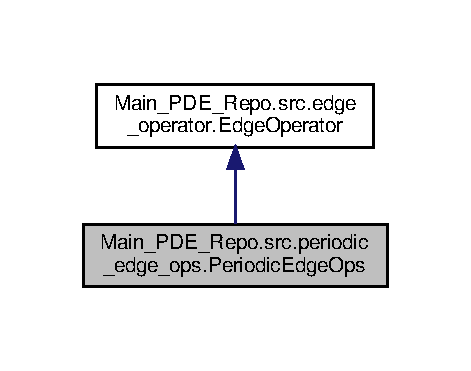
\includegraphics[width=226pt]{classMain__PDE__Repo_1_1src_1_1periodic__edge__ops_1_1PeriodicEdgeOps__inherit__graph}
\end{center}
\end{figure}


Collaboration diagram for Main\+\_\+\+P\+D\+E\+\_\+\+Repo.\+src.\+periodic\+\_\+edge\+\_\+ops.\+Periodic\+Edge\+Ops\+:
\nopagebreak
\begin{figure}[H]
\begin{center}
\leavevmode
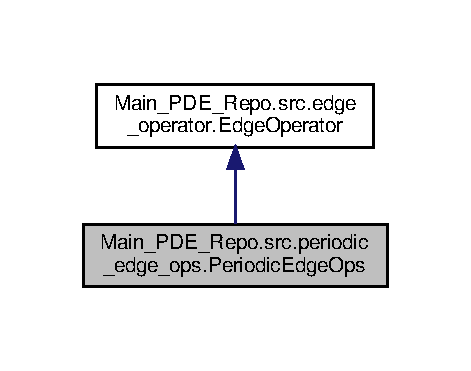
\includegraphics[width=226pt]{classMain__PDE__Repo_1_1src_1_1periodic__edge__ops_1_1PeriodicEdgeOps__coll__graph}
\end{center}
\end{figure}
\subsection*{Public Member Functions}
\begin{DoxyCompactItemize}
\item 
def \hyperlink{classMain__PDE__Repo_1_1src_1_1periodic__edge__ops_1_1PeriodicEdgeOps_a53de9ebf1511a71d9c395e89af86c301}{\+\_\+\+\_\+init\+\_\+\+\_\+} (self)
\begin{DoxyCompactList}\small\item\em The constructor. \end{DoxyCompactList}\end{DoxyCompactItemize}
\subsection*{Public Attributes}
\begin{DoxyCompactItemize}
\item 
\hyperlink{classMain__PDE__Repo_1_1src_1_1periodic__edge__ops_1_1PeriodicEdgeOps_a1ae9e7005e5213be99bf207e3cd533ef}{name}
\end{DoxyCompactItemize}
\subsection*{Private Member Functions}
\begin{DoxyCompactItemize}
\item 
def \hyperlink{classMain__PDE__Repo_1_1src_1_1periodic__edge__ops_1_1PeriodicEdgeOps_a85e9e091c9c3d4e027ff4d3a3acb368d}{\+\_\+set\+\_\+name} (self)
\end{DoxyCompactItemize}


\subsection{Detailed Description}
The periodic edge operator subclass of edge operator will handle the operators applied to grid edges with periodic boundary conditions in the evaluation of the R\+HS of the P\+DE. 



\subsection{Constructor \& Destructor Documentation}
\mbox{\Hypertarget{classMain__PDE__Repo_1_1src_1_1periodic__edge__ops_1_1PeriodicEdgeOps_a53de9ebf1511a71d9c395e89af86c301}\label{classMain__PDE__Repo_1_1src_1_1periodic__edge__ops_1_1PeriodicEdgeOps_a53de9ebf1511a71d9c395e89af86c301}} 
\index{Main\+\_\+\+P\+D\+E\+\_\+\+Repo\+::src\+::periodic\+\_\+edge\+\_\+ops\+::\+Periodic\+Edge\+Ops@{Main\+\_\+\+P\+D\+E\+\_\+\+Repo\+::src\+::periodic\+\_\+edge\+\_\+ops\+::\+Periodic\+Edge\+Ops}!\+\_\+\+\_\+init\+\_\+\+\_\+@{\+\_\+\+\_\+init\+\_\+\+\_\+}}
\index{\+\_\+\+\_\+init\+\_\+\+\_\+@{\+\_\+\+\_\+init\+\_\+\+\_\+}!Main\+\_\+\+P\+D\+E\+\_\+\+Repo\+::src\+::periodic\+\_\+edge\+\_\+ops\+::\+Periodic\+Edge\+Ops@{Main\+\_\+\+P\+D\+E\+\_\+\+Repo\+::src\+::periodic\+\_\+edge\+\_\+ops\+::\+Periodic\+Edge\+Ops}}
\subsubsection{\texorpdfstring{\+\_\+\+\_\+init\+\_\+\+\_\+()}{\_\_init\_\_()}}
{\footnotesize\ttfamily def Main\+\_\+\+P\+D\+E\+\_\+\+Repo.\+src.\+periodic\+\_\+edge\+\_\+ops.\+Periodic\+Edge\+Ops.\+\_\+\+\_\+init\+\_\+\+\_\+ (\begin{DoxyParamCaption}\item[{}]{self }\end{DoxyParamCaption})}



The constructor. 



\subsection{Member Function Documentation}
\mbox{\Hypertarget{classMain__PDE__Repo_1_1src_1_1periodic__edge__ops_1_1PeriodicEdgeOps_a85e9e091c9c3d4e027ff4d3a3acb368d}\label{classMain__PDE__Repo_1_1src_1_1periodic__edge__ops_1_1PeriodicEdgeOps_a85e9e091c9c3d4e027ff4d3a3acb368d}} 
\index{Main\+\_\+\+P\+D\+E\+\_\+\+Repo\+::src\+::periodic\+\_\+edge\+\_\+ops\+::\+Periodic\+Edge\+Ops@{Main\+\_\+\+P\+D\+E\+\_\+\+Repo\+::src\+::periodic\+\_\+edge\+\_\+ops\+::\+Periodic\+Edge\+Ops}!\+\_\+set\+\_\+name@{\+\_\+set\+\_\+name}}
\index{\+\_\+set\+\_\+name@{\+\_\+set\+\_\+name}!Main\+\_\+\+P\+D\+E\+\_\+\+Repo\+::src\+::periodic\+\_\+edge\+\_\+ops\+::\+Periodic\+Edge\+Ops@{Main\+\_\+\+P\+D\+E\+\_\+\+Repo\+::src\+::periodic\+\_\+edge\+\_\+ops\+::\+Periodic\+Edge\+Ops}}
\subsubsection{\texorpdfstring{\+\_\+set\+\_\+name()}{\_set\_name()}}
{\footnotesize\ttfamily def Main\+\_\+\+P\+D\+E\+\_\+\+Repo.\+src.\+periodic\+\_\+edge\+\_\+ops.\+Periodic\+Edge\+Ops.\+\_\+set\+\_\+name (\begin{DoxyParamCaption}\item[{}]{self }\end{DoxyParamCaption})\hspace{0.3cm}{\ttfamily [private]}}



\subsection{Member Data Documentation}
\mbox{\Hypertarget{classMain__PDE__Repo_1_1src_1_1periodic__edge__ops_1_1PeriodicEdgeOps_a1ae9e7005e5213be99bf207e3cd533ef}\label{classMain__PDE__Repo_1_1src_1_1periodic__edge__ops_1_1PeriodicEdgeOps_a1ae9e7005e5213be99bf207e3cd533ef}} 
\index{Main\+\_\+\+P\+D\+E\+\_\+\+Repo\+::src\+::periodic\+\_\+edge\+\_\+ops\+::\+Periodic\+Edge\+Ops@{Main\+\_\+\+P\+D\+E\+\_\+\+Repo\+::src\+::periodic\+\_\+edge\+\_\+ops\+::\+Periodic\+Edge\+Ops}!name@{name}}
\index{name@{name}!Main\+\_\+\+P\+D\+E\+\_\+\+Repo\+::src\+::periodic\+\_\+edge\+\_\+ops\+::\+Periodic\+Edge\+Ops@{Main\+\_\+\+P\+D\+E\+\_\+\+Repo\+::src\+::periodic\+\_\+edge\+\_\+ops\+::\+Periodic\+Edge\+Ops}}
\subsubsection{\texorpdfstring{name}{name}}
{\footnotesize\ttfamily Main\+\_\+\+P\+D\+E\+\_\+\+Repo.\+src.\+periodic\+\_\+edge\+\_\+ops.\+Periodic\+Edge\+Ops.\+name}



The documentation for this class was generated from the following file\+:\begin{DoxyCompactItemize}
\item 
src/\hyperlink{periodic__edge__ops_8py}{periodic\+\_\+edge\+\_\+ops.\+py}\end{DoxyCompactItemize}

\hypertarget{classMain__PDE__Repo_1_1src_1_1plot__end_1_1PlotEnd}{}\section{Main\+\_\+\+P\+D\+E\+\_\+\+Repo.\+src.\+plot\+\_\+end.\+Plot\+End Class Reference}
\label{classMain__PDE__Repo_1_1src_1_1plot__end_1_1PlotEnd}\index{Main\+\_\+\+P\+D\+E\+\_\+\+Repo.\+src.\+plot\+\_\+end.\+Plot\+End@{Main\+\_\+\+P\+D\+E\+\_\+\+Repo.\+src.\+plot\+\_\+end.\+Plot\+End}}


P\+Lot\+End Implementation of \hyperlink{namespaceMain__PDE__Repo_1_1src_1_1plot__end}{plot\+\_\+end} package as a class.  




Inheritance diagram for Main\+\_\+\+P\+D\+E\+\_\+\+Repo.\+src.\+plot\+\_\+end.\+Plot\+End\+:
\nopagebreak
\begin{figure}[H]
\begin{center}
\leavevmode
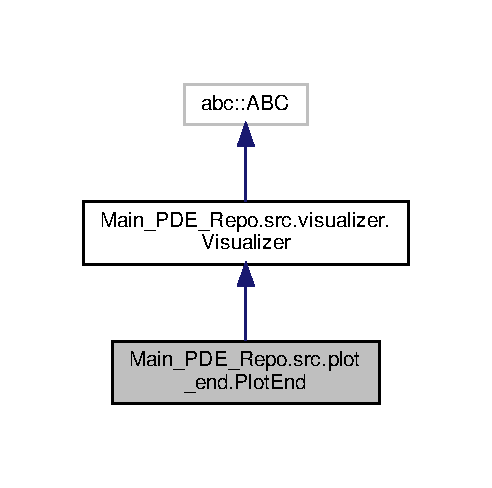
\includegraphics[width=236pt]{classMain__PDE__Repo_1_1src_1_1plot__end_1_1PlotEnd__inherit__graph}
\end{center}
\end{figure}


Collaboration diagram for Main\+\_\+\+P\+D\+E\+\_\+\+Repo.\+src.\+plot\+\_\+end.\+Plot\+End\+:
\nopagebreak
\begin{figure}[H]
\begin{center}
\leavevmode
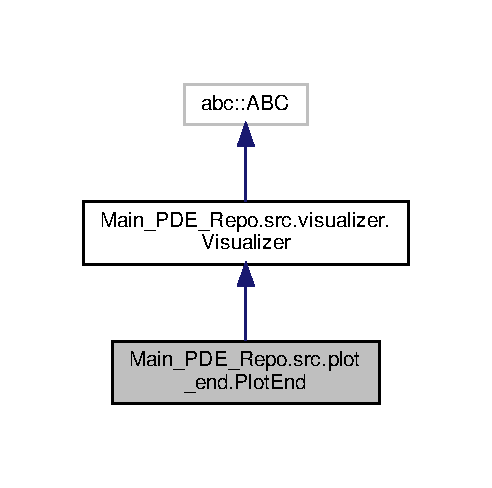
\includegraphics[width=236pt]{classMain__PDE__Repo_1_1src_1_1plot__end_1_1PlotEnd__coll__graph}
\end{center}
\end{figure}
\subsection*{Public Member Functions}
\begin{DoxyCompactItemize}
\item 
def \hyperlink{classMain__PDE__Repo_1_1src_1_1plot__end_1_1PlotEnd_ab7d1c0200dfbb81b6d47bbfbf7c0737e}{\+\_\+\+\_\+init\+\_\+\+\_\+} (self, \hyperlink{classMain__PDE__Repo_1_1src_1_1plot__end_1_1PlotEnd_a86821453d070a209c99b4133615f529c}{outloc})
\begin{DoxyCompactList}\small\item\em Constructor. \end{DoxyCompactList}\item 
def \hyperlink{classMain__PDE__Repo_1_1src_1_1plot__end_1_1PlotEnd_a9656ba2b4cb0f900ef16f5fc4ef58a68}{plot1d} (self, log, name=\char`\"{}\char`\"{}, kwargs)
\begin{DoxyCompactList}\small\item\em plot1d class to plot first and last frames of a 1d grid held in a logger \end{DoxyCompactList}\item 
def \hyperlink{classMain__PDE__Repo_1_1src_1_1plot__end_1_1PlotEnd_a968b35790b6c73b8e8f91b7a505be56e}{plot2d} (self, log, name=\char`\"{}\char`\"{}, kwargs)
\begin{DoxyCompactList}\small\item\em plot2d class to plot first and last frames of a 2d grid held in a logger \end{DoxyCompactList}\end{DoxyCompactItemize}
\subsection*{Public Attributes}
\begin{DoxyCompactItemize}
\item 
\hyperlink{classMain__PDE__Repo_1_1src_1_1plot__end_1_1PlotEnd_a86821453d070a209c99b4133615f529c}{outloc}
\end{DoxyCompactItemize}


\subsection{Detailed Description}
P\+Lot\+End Implementation of \hyperlink{namespaceMain__PDE__Repo_1_1src_1_1plot__end}{plot\+\_\+end} package as a class. 

\subsection{Constructor \& Destructor Documentation}
\mbox{\Hypertarget{classMain__PDE__Repo_1_1src_1_1plot__end_1_1PlotEnd_ab7d1c0200dfbb81b6d47bbfbf7c0737e}\label{classMain__PDE__Repo_1_1src_1_1plot__end_1_1PlotEnd_ab7d1c0200dfbb81b6d47bbfbf7c0737e}} 
\index{Main\+\_\+\+P\+D\+E\+\_\+\+Repo\+::src\+::plot\+\_\+end\+::\+Plot\+End@{Main\+\_\+\+P\+D\+E\+\_\+\+Repo\+::src\+::plot\+\_\+end\+::\+Plot\+End}!\+\_\+\+\_\+init\+\_\+\+\_\+@{\+\_\+\+\_\+init\+\_\+\+\_\+}}
\index{\+\_\+\+\_\+init\+\_\+\+\_\+@{\+\_\+\+\_\+init\+\_\+\+\_\+}!Main\+\_\+\+P\+D\+E\+\_\+\+Repo\+::src\+::plot\+\_\+end\+::\+Plot\+End@{Main\+\_\+\+P\+D\+E\+\_\+\+Repo\+::src\+::plot\+\_\+end\+::\+Plot\+End}}
\subsubsection{\texorpdfstring{\+\_\+\+\_\+init\+\_\+\+\_\+()}{\_\_init\_\_()}}
{\footnotesize\ttfamily def Main\+\_\+\+P\+D\+E\+\_\+\+Repo.\+src.\+plot\+\_\+end.\+Plot\+End.\+\_\+\+\_\+init\+\_\+\+\_\+ (\begin{DoxyParamCaption}\item[{}]{self,  }\item[{}]{outloc }\end{DoxyParamCaption})}



Constructor. 


\begin{DoxyParams}{Parameters}
{\em outloc} & directory name for output to be saved to \\
\hline
\end{DoxyParams}


\subsection{Member Function Documentation}
\mbox{\Hypertarget{classMain__PDE__Repo_1_1src_1_1plot__end_1_1PlotEnd_a9656ba2b4cb0f900ef16f5fc4ef58a68}\label{classMain__PDE__Repo_1_1src_1_1plot__end_1_1PlotEnd_a9656ba2b4cb0f900ef16f5fc4ef58a68}} 
\index{Main\+\_\+\+P\+D\+E\+\_\+\+Repo\+::src\+::plot\+\_\+end\+::\+Plot\+End@{Main\+\_\+\+P\+D\+E\+\_\+\+Repo\+::src\+::plot\+\_\+end\+::\+Plot\+End}!plot1d@{plot1d}}
\index{plot1d@{plot1d}!Main\+\_\+\+P\+D\+E\+\_\+\+Repo\+::src\+::plot\+\_\+end\+::\+Plot\+End@{Main\+\_\+\+P\+D\+E\+\_\+\+Repo\+::src\+::plot\+\_\+end\+::\+Plot\+End}}
\subsubsection{\texorpdfstring{plot1d()}{plot1d()}}
{\footnotesize\ttfamily def Main\+\_\+\+P\+D\+E\+\_\+\+Repo.\+src.\+plot\+\_\+end.\+Plot\+End.\+plot1d (\begin{DoxyParamCaption}\item[{}]{self,  }\item[{}]{log,  }\item[{}]{name = {\ttfamily \char`\"{}\char`\"{}},  }\item[{}]{kwargs }\end{DoxyParamCaption})}



plot1d class to plot first and last frames of a 1d grid held in a logger 

plots a 1d contour of the first and last frames of the P\+DE solution and saves them to the outputs director uses matplotlib to actually generate the plots 
\begin{DoxyParams}{Parameters}
{\em log} & a Logger() object \\
\hline
{\em name} & a string containing the desired name of the file \\
\hline
{\em $\ast$$\ast$kwargs} & keyword arguments that will be passed to the plt.\+plot function \\
\hline
\end{DoxyParams}
\mbox{\Hypertarget{classMain__PDE__Repo_1_1src_1_1plot__end_1_1PlotEnd_a968b35790b6c73b8e8f91b7a505be56e}\label{classMain__PDE__Repo_1_1src_1_1plot__end_1_1PlotEnd_a968b35790b6c73b8e8f91b7a505be56e}} 
\index{Main\+\_\+\+P\+D\+E\+\_\+\+Repo\+::src\+::plot\+\_\+end\+::\+Plot\+End@{Main\+\_\+\+P\+D\+E\+\_\+\+Repo\+::src\+::plot\+\_\+end\+::\+Plot\+End}!plot2d@{plot2d}}
\index{plot2d@{plot2d}!Main\+\_\+\+P\+D\+E\+\_\+\+Repo\+::src\+::plot\+\_\+end\+::\+Plot\+End@{Main\+\_\+\+P\+D\+E\+\_\+\+Repo\+::src\+::plot\+\_\+end\+::\+Plot\+End}}
\subsubsection{\texorpdfstring{plot2d()}{plot2d()}}
{\footnotesize\ttfamily def Main\+\_\+\+P\+D\+E\+\_\+\+Repo.\+src.\+plot\+\_\+end.\+Plot\+End.\+plot2d (\begin{DoxyParamCaption}\item[{}]{self,  }\item[{}]{log,  }\item[{}]{name = {\ttfamily \char`\"{}\char`\"{}},  }\item[{}]{kwargs }\end{DoxyParamCaption})}



plot2d class to plot first and last frames of a 2d grid held in a logger 

plots a 2d contour of the first and last frames of the P\+DE solution and saves them to the outputs director uses matplotlib to actually generate the plots 
\begin{DoxyParams}{Parameters}
{\em log} & a Logger() object \\
\hline
{\em name} & a string containing the desired name of the file \\
\hline
{\em $\ast$$\ast$kwargs} & keyword arguments that will be passed to the plt.\+contourf function \\
\hline
\end{DoxyParams}


\subsection{Member Data Documentation}
\mbox{\Hypertarget{classMain__PDE__Repo_1_1src_1_1plot__end_1_1PlotEnd_a86821453d070a209c99b4133615f529c}\label{classMain__PDE__Repo_1_1src_1_1plot__end_1_1PlotEnd_a86821453d070a209c99b4133615f529c}} 
\index{Main\+\_\+\+P\+D\+E\+\_\+\+Repo\+::src\+::plot\+\_\+end\+::\+Plot\+End@{Main\+\_\+\+P\+D\+E\+\_\+\+Repo\+::src\+::plot\+\_\+end\+::\+Plot\+End}!outloc@{outloc}}
\index{outloc@{outloc}!Main\+\_\+\+P\+D\+E\+\_\+\+Repo\+::src\+::plot\+\_\+end\+::\+Plot\+End@{Main\+\_\+\+P\+D\+E\+\_\+\+Repo\+::src\+::plot\+\_\+end\+::\+Plot\+End}}
\subsubsection{\texorpdfstring{outloc}{outloc}}
{\footnotesize\ttfamily Main\+\_\+\+P\+D\+E\+\_\+\+Repo.\+src.\+plot\+\_\+end.\+Plot\+End.\+outloc}



The documentation for this class was generated from the following file\+:\begin{DoxyCompactItemize}
\item 
src/\hyperlink{plot__end_8py}{plot\+\_\+end.\+py}\end{DoxyCompactItemize}

\hypertarget{classMain__PDE__Repo_1_1src_1_1populator_1_1Populator}{}\section{Main\+\_\+\+P\+D\+E\+\_\+\+Repo.\+src.\+populator.\+Populator Class Reference}
\label{classMain__PDE__Repo_1_1src_1_1populator_1_1Populator}\index{Main\+\_\+\+P\+D\+E\+\_\+\+Repo.\+src.\+populator.\+Populator@{Main\+\_\+\+P\+D\+E\+\_\+\+Repo.\+src.\+populator.\+Populator}}


\hyperlink{classMain__PDE__Repo_1_1src_1_1populator_1_1Populator}{Populator} Function to populate an op\+\_\+matrix according to a particular 1d operator.  


\subsection*{Public Member Functions}
\begin{DoxyCompactItemize}
\item 
def \hyperlink{classMain__PDE__Repo_1_1src_1_1populator_1_1Populator_a2bf19f9a4fdf912a755f2ba62a583c8f}{\+\_\+\+\_\+init\+\_\+\+\_\+} (self, spec, \hyperlink{classMain__PDE__Repo_1_1src_1_1populator_1_1Populator_a301b505c724a5a9c3f446f2260a69469}{dim})
\item 
def \hyperlink{classMain__PDE__Repo_1_1src_1_1populator_1_1Populator_adedc630ce47f1836ea4d7321b87ff3cd}{populate\+\_\+op} (self, mesh, op\+\_\+mat, op1d)
\end{DoxyCompactItemize}
\subsection*{Public Attributes}
\begin{DoxyCompactItemize}
\item 
\hyperlink{classMain__PDE__Repo_1_1src_1_1populator_1_1Populator_af9e860df7e6784efab29a3f3677a6728}{shape}
\item 
\hyperlink{classMain__PDE__Repo_1_1src_1_1populator_1_1Populator_a301b505c724a5a9c3f446f2260a69469}{dim}
\item 
\hyperlink{classMain__PDE__Repo_1_1src_1_1populator_1_1Populator_abca46171554ca659807610d0c53c8d5d}{dx}
\end{DoxyCompactItemize}
\subsection*{Private Member Functions}
\begin{DoxyCompactItemize}
\item 
def \hyperlink{classMain__PDE__Repo_1_1src_1_1populator_1_1Populator_ab94a2b5767f776c3a4b62b161a071828}{\+\_\+set\+\_\+row} (self, op1d, coords, op\+\_\+mat, op\+\_\+index)
\item 
def \hyperlink{classMain__PDE__Repo_1_1src_1_1populator_1_1Populator_aabb6d0bae97c41cc83ec81dd5f958fa3}{\+\_\+get\+\_\+single\+\_\+index} (self, coords)
\begin{DoxyCompactList}\small\item\em \+\_\+get\+\_\+single\+\_\+index Generates a single flattened index for an n-\/dimensional grid position. \end{DoxyCompactList}\end{DoxyCompactItemize}


\subsection{Detailed Description}
\hyperlink{classMain__PDE__Repo_1_1src_1_1populator_1_1Populator}{Populator} Function to populate an op\+\_\+matrix according to a particular 1d operator. 

C\+Lass can take a 1d operator and a portion of a grid to generate FD values for each index in a matrix operator that can then calculate that finite difference. 

\subsection{Constructor \& Destructor Documentation}
\mbox{\Hypertarget{classMain__PDE__Repo_1_1src_1_1populator_1_1Populator_a2bf19f9a4fdf912a755f2ba62a583c8f}\label{classMain__PDE__Repo_1_1src_1_1populator_1_1Populator_a2bf19f9a4fdf912a755f2ba62a583c8f}} 
\index{Main\+\_\+\+P\+D\+E\+\_\+\+Repo\+::src\+::populator\+::\+Populator@{Main\+\_\+\+P\+D\+E\+\_\+\+Repo\+::src\+::populator\+::\+Populator}!\+\_\+\+\_\+init\+\_\+\+\_\+@{\+\_\+\+\_\+init\+\_\+\+\_\+}}
\index{\+\_\+\+\_\+init\+\_\+\+\_\+@{\+\_\+\+\_\+init\+\_\+\+\_\+}!Main\+\_\+\+P\+D\+E\+\_\+\+Repo\+::src\+::populator\+::\+Populator@{Main\+\_\+\+P\+D\+E\+\_\+\+Repo\+::src\+::populator\+::\+Populator}}
\subsubsection{\texorpdfstring{\+\_\+\+\_\+init\+\_\+\+\_\+()}{\_\_init\_\_()}}
{\footnotesize\ttfamily def Main\+\_\+\+P\+D\+E\+\_\+\+Repo.\+src.\+populator.\+Populator.\+\_\+\+\_\+init\+\_\+\+\_\+ (\begin{DoxyParamCaption}\item[{}]{self,  }\item[{}]{spec,  }\item[{}]{dim }\end{DoxyParamCaption})}



\subsection{Member Function Documentation}
\mbox{\Hypertarget{classMain__PDE__Repo_1_1src_1_1populator_1_1Populator_aabb6d0bae97c41cc83ec81dd5f958fa3}\label{classMain__PDE__Repo_1_1src_1_1populator_1_1Populator_aabb6d0bae97c41cc83ec81dd5f958fa3}} 
\index{Main\+\_\+\+P\+D\+E\+\_\+\+Repo\+::src\+::populator\+::\+Populator@{Main\+\_\+\+P\+D\+E\+\_\+\+Repo\+::src\+::populator\+::\+Populator}!\+\_\+get\+\_\+single\+\_\+index@{\+\_\+get\+\_\+single\+\_\+index}}
\index{\+\_\+get\+\_\+single\+\_\+index@{\+\_\+get\+\_\+single\+\_\+index}!Main\+\_\+\+P\+D\+E\+\_\+\+Repo\+::src\+::populator\+::\+Populator@{Main\+\_\+\+P\+D\+E\+\_\+\+Repo\+::src\+::populator\+::\+Populator}}
\subsubsection{\texorpdfstring{\+\_\+get\+\_\+single\+\_\+index()}{\_get\_single\_index()}}
{\footnotesize\ttfamily def Main\+\_\+\+P\+D\+E\+\_\+\+Repo.\+src.\+populator.\+Populator.\+\_\+get\+\_\+single\+\_\+index (\begin{DoxyParamCaption}\item[{}]{self,  }\item[{}]{coords }\end{DoxyParamCaption})\hspace{0.3cm}{\ttfamily [private]}}



\+\_\+get\+\_\+single\+\_\+index Generates a single flattened index for an n-\/dimensional grid position. 

Private method which returns the corresponding to a particular set of n-\/dimensional coordinates specifying location on a grid.  coords A list of coordinates with length equal to length(self.\+shape).  index The index corresponding to a row-\/major flattening operation applied to the n-\/dimensional matrix to express it as a 1D matrix. \mbox{\Hypertarget{classMain__PDE__Repo_1_1src_1_1populator_1_1Populator_ab94a2b5767f776c3a4b62b161a071828}\label{classMain__PDE__Repo_1_1src_1_1populator_1_1Populator_ab94a2b5767f776c3a4b62b161a071828}} 
\index{Main\+\_\+\+P\+D\+E\+\_\+\+Repo\+::src\+::populator\+::\+Populator@{Main\+\_\+\+P\+D\+E\+\_\+\+Repo\+::src\+::populator\+::\+Populator}!\+\_\+set\+\_\+row@{\+\_\+set\+\_\+row}}
\index{\+\_\+set\+\_\+row@{\+\_\+set\+\_\+row}!Main\+\_\+\+P\+D\+E\+\_\+\+Repo\+::src\+::populator\+::\+Populator@{Main\+\_\+\+P\+D\+E\+\_\+\+Repo\+::src\+::populator\+::\+Populator}}
\subsubsection{\texorpdfstring{\+\_\+set\+\_\+row()}{\_set\_row()}}
{\footnotesize\ttfamily def Main\+\_\+\+P\+D\+E\+\_\+\+Repo.\+src.\+populator.\+Populator.\+\_\+set\+\_\+row (\begin{DoxyParamCaption}\item[{}]{self,  }\item[{}]{op1d,  }\item[{}]{coords,  }\item[{}]{op\+\_\+mat,  }\item[{}]{op\+\_\+index }\end{DoxyParamCaption})\hspace{0.3cm}{\ttfamily [private]}}

\mbox{\Hypertarget{classMain__PDE__Repo_1_1src_1_1populator_1_1Populator_adedc630ce47f1836ea4d7321b87ff3cd}\label{classMain__PDE__Repo_1_1src_1_1populator_1_1Populator_adedc630ce47f1836ea4d7321b87ff3cd}} 
\index{Main\+\_\+\+P\+D\+E\+\_\+\+Repo\+::src\+::populator\+::\+Populator@{Main\+\_\+\+P\+D\+E\+\_\+\+Repo\+::src\+::populator\+::\+Populator}!populate\+\_\+op@{populate\+\_\+op}}
\index{populate\+\_\+op@{populate\+\_\+op}!Main\+\_\+\+P\+D\+E\+\_\+\+Repo\+::src\+::populator\+::\+Populator@{Main\+\_\+\+P\+D\+E\+\_\+\+Repo\+::src\+::populator\+::\+Populator}}
\subsubsection{\texorpdfstring{populate\+\_\+op()}{populate\_op()}}
{\footnotesize\ttfamily def Main\+\_\+\+P\+D\+E\+\_\+\+Repo.\+src.\+populator.\+Populator.\+populate\+\_\+op (\begin{DoxyParamCaption}\item[{}]{self,  }\item[{}]{mesh,  }\item[{}]{op\+\_\+mat,  }\item[{}]{op1d }\end{DoxyParamCaption})}



\subsection{Member Data Documentation}
\mbox{\Hypertarget{classMain__PDE__Repo_1_1src_1_1populator_1_1Populator_a301b505c724a5a9c3f446f2260a69469}\label{classMain__PDE__Repo_1_1src_1_1populator_1_1Populator_a301b505c724a5a9c3f446f2260a69469}} 
\index{Main\+\_\+\+P\+D\+E\+\_\+\+Repo\+::src\+::populator\+::\+Populator@{Main\+\_\+\+P\+D\+E\+\_\+\+Repo\+::src\+::populator\+::\+Populator}!dim@{dim}}
\index{dim@{dim}!Main\+\_\+\+P\+D\+E\+\_\+\+Repo\+::src\+::populator\+::\+Populator@{Main\+\_\+\+P\+D\+E\+\_\+\+Repo\+::src\+::populator\+::\+Populator}}
\subsubsection{\texorpdfstring{dim}{dim}}
{\footnotesize\ttfamily Main\+\_\+\+P\+D\+E\+\_\+\+Repo.\+src.\+populator.\+Populator.\+dim}

\mbox{\Hypertarget{classMain__PDE__Repo_1_1src_1_1populator_1_1Populator_abca46171554ca659807610d0c53c8d5d}\label{classMain__PDE__Repo_1_1src_1_1populator_1_1Populator_abca46171554ca659807610d0c53c8d5d}} 
\index{Main\+\_\+\+P\+D\+E\+\_\+\+Repo\+::src\+::populator\+::\+Populator@{Main\+\_\+\+P\+D\+E\+\_\+\+Repo\+::src\+::populator\+::\+Populator}!dx@{dx}}
\index{dx@{dx}!Main\+\_\+\+P\+D\+E\+\_\+\+Repo\+::src\+::populator\+::\+Populator@{Main\+\_\+\+P\+D\+E\+\_\+\+Repo\+::src\+::populator\+::\+Populator}}
\subsubsection{\texorpdfstring{dx}{dx}}
{\footnotesize\ttfamily Main\+\_\+\+P\+D\+E\+\_\+\+Repo.\+src.\+populator.\+Populator.\+dx}

\mbox{\Hypertarget{classMain__PDE__Repo_1_1src_1_1populator_1_1Populator_af9e860df7e6784efab29a3f3677a6728}\label{classMain__PDE__Repo_1_1src_1_1populator_1_1Populator_af9e860df7e6784efab29a3f3677a6728}} 
\index{Main\+\_\+\+P\+D\+E\+\_\+\+Repo\+::src\+::populator\+::\+Populator@{Main\+\_\+\+P\+D\+E\+\_\+\+Repo\+::src\+::populator\+::\+Populator}!shape@{shape}}
\index{shape@{shape}!Main\+\_\+\+P\+D\+E\+\_\+\+Repo\+::src\+::populator\+::\+Populator@{Main\+\_\+\+P\+D\+E\+\_\+\+Repo\+::src\+::populator\+::\+Populator}}
\subsubsection{\texorpdfstring{shape}{shape}}
{\footnotesize\ttfamily Main\+\_\+\+P\+D\+E\+\_\+\+Repo.\+src.\+populator.\+Populator.\+shape}



The documentation for this class was generated from the following file\+:\begin{DoxyCompactItemize}
\item 
src/\hyperlink{populator_8py}{populator.\+py}\end{DoxyCompactItemize}

\hypertarget{classMain__PDE__Repo_1_1src_1_1problem_1_1Problem}{}\section{Main\+\_\+\+P\+D\+E\+\_\+\+Repo.\+src.\+problem.\+Problem Class Reference}
\label{classMain__PDE__Repo_1_1src_1_1problem_1_1Problem}\index{Main\+\_\+\+P\+D\+E\+\_\+\+Repo.\+src.\+problem.\+Problem@{Main\+\_\+\+P\+D\+E\+\_\+\+Repo.\+src.\+problem.\+Problem}}


The abstract \hyperlink{classMain__PDE__Repo_1_1src_1_1problem_1_1Problem}{Problem} class.  




Inheritance diagram for Main\+\_\+\+P\+D\+E\+\_\+\+Repo.\+src.\+problem.\+Problem\+:
\nopagebreak
\begin{figure}[H]
\begin{center}
\leavevmode
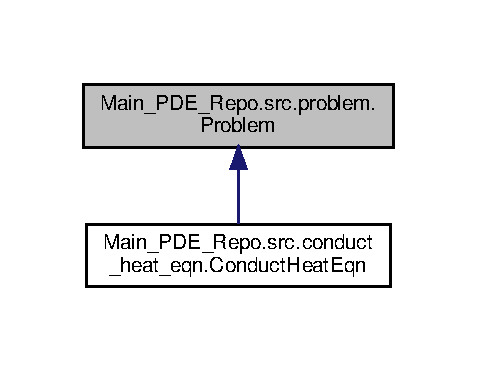
\includegraphics[width=229pt]{classMain__PDE__Repo_1_1src_1_1problem_1_1Problem__inherit__graph}
\end{center}
\end{figure}
\subsection*{Public Member Functions}
\begin{DoxyCompactItemize}
\item 
def \hyperlink{classMain__PDE__Repo_1_1src_1_1problem_1_1Problem_a3bd7ab602ec2348c69edcfc82fc35794}{\+\_\+\+\_\+init\+\_\+\+\_\+} (self)
\begin{DoxyCompactList}\small\item\em The constructor initializes the problem with operator members and constant parameter members. \end{DoxyCompactList}\item 
def \hyperlink{classMain__PDE__Repo_1_1src_1_1problem_1_1Problem_a1885fe3e15581db4feda8af513ae91e5}{R\+HS} (self)
\begin{DoxyCompactList}\small\item\em The R\+HS function applies the defined operators to the grid argument in a defined manner. \end{DoxyCompactList}\item 
def \hyperlink{classMain__PDE__Repo_1_1src_1_1problem_1_1Problem_aeaea1beb92b43dde42d5175ddde1f276}{set\+\_\+ops} (self)
\begin{DoxyCompactList}\small\item\em The set\+\_\+ops function takes a dictionary of linear operators defined elsewhere and sets them to the correct member variables in the problem. \end{DoxyCompactList}\item 
def \hyperlink{classMain__PDE__Repo_1_1src_1_1problem_1_1Problem_a8b13459d6f5c9709f6dc647caf6c0d5c}{set\+\_\+\+B\+Cs} (self)
\begin{DoxyCompactList}\small\item\em Call the boundary handler to set the boundary values. \end{DoxyCompactList}\end{DoxyCompactItemize}
\subsection*{Public Attributes}
\begin{DoxyCompactItemize}
\item 
\hyperlink{classMain__PDE__Repo_1_1src_1_1problem_1_1Problem_a7700a3b18e39488fbe81a8fb06ebb982}{ops\+\_\+set\+\_\+flag}
\item 
\hyperlink{classMain__PDE__Repo_1_1src_1_1problem_1_1Problem_a7736044b7f2938008a30043000e62f87}{ops}
\end{DoxyCompactItemize}


\subsection{Detailed Description}
The abstract \hyperlink{classMain__PDE__Repo_1_1src_1_1problem_1_1Problem}{Problem} class. 

Concrete sublclasses define the constant parameters and R\+HS function operators 

\subsection{Constructor \& Destructor Documentation}
\mbox{\Hypertarget{classMain__PDE__Repo_1_1src_1_1problem_1_1Problem_a3bd7ab602ec2348c69edcfc82fc35794}\label{classMain__PDE__Repo_1_1src_1_1problem_1_1Problem_a3bd7ab602ec2348c69edcfc82fc35794}} 
\index{Main\+\_\+\+P\+D\+E\+\_\+\+Repo\+::src\+::problem\+::\+Problem@{Main\+\_\+\+P\+D\+E\+\_\+\+Repo\+::src\+::problem\+::\+Problem}!\+\_\+\+\_\+init\+\_\+\+\_\+@{\+\_\+\+\_\+init\+\_\+\+\_\+}}
\index{\+\_\+\+\_\+init\+\_\+\+\_\+@{\+\_\+\+\_\+init\+\_\+\+\_\+}!Main\+\_\+\+P\+D\+E\+\_\+\+Repo\+::src\+::problem\+::\+Problem@{Main\+\_\+\+P\+D\+E\+\_\+\+Repo\+::src\+::problem\+::\+Problem}}
\subsubsection{\texorpdfstring{\+\_\+\+\_\+init\+\_\+\+\_\+()}{\_\_init\_\_()}}
{\footnotesize\ttfamily def Main\+\_\+\+P\+D\+E\+\_\+\+Repo.\+src.\+problem.\+Problem.\+\_\+\+\_\+init\+\_\+\+\_\+ (\begin{DoxyParamCaption}\item[{}]{self }\end{DoxyParamCaption})}



The constructor initializes the problem with operator members and constant parameter members. 



\subsection{Member Function Documentation}
\mbox{\Hypertarget{classMain__PDE__Repo_1_1src_1_1problem_1_1Problem_a1885fe3e15581db4feda8af513ae91e5}\label{classMain__PDE__Repo_1_1src_1_1problem_1_1Problem_a1885fe3e15581db4feda8af513ae91e5}} 
\index{Main\+\_\+\+P\+D\+E\+\_\+\+Repo\+::src\+::problem\+::\+Problem@{Main\+\_\+\+P\+D\+E\+\_\+\+Repo\+::src\+::problem\+::\+Problem}!R\+HS@{R\+HS}}
\index{R\+HS@{R\+HS}!Main\+\_\+\+P\+D\+E\+\_\+\+Repo\+::src\+::problem\+::\+Problem@{Main\+\_\+\+P\+D\+E\+\_\+\+Repo\+::src\+::problem\+::\+Problem}}
\subsubsection{\texorpdfstring{R\+H\+S()}{RHS()}}
{\footnotesize\ttfamily def Main\+\_\+\+P\+D\+E\+\_\+\+Repo.\+src.\+problem.\+Problem.\+R\+HS (\begin{DoxyParamCaption}\item[{}]{self }\end{DoxyParamCaption})}



The R\+HS function applies the defined operators to the grid argument in a defined manner. 

\mbox{\Hypertarget{classMain__PDE__Repo_1_1src_1_1problem_1_1Problem_a8b13459d6f5c9709f6dc647caf6c0d5c}\label{classMain__PDE__Repo_1_1src_1_1problem_1_1Problem_a8b13459d6f5c9709f6dc647caf6c0d5c}} 
\index{Main\+\_\+\+P\+D\+E\+\_\+\+Repo\+::src\+::problem\+::\+Problem@{Main\+\_\+\+P\+D\+E\+\_\+\+Repo\+::src\+::problem\+::\+Problem}!set\+\_\+\+B\+Cs@{set\+\_\+\+B\+Cs}}
\index{set\+\_\+\+B\+Cs@{set\+\_\+\+B\+Cs}!Main\+\_\+\+P\+D\+E\+\_\+\+Repo\+::src\+::problem\+::\+Problem@{Main\+\_\+\+P\+D\+E\+\_\+\+Repo\+::src\+::problem\+::\+Problem}}
\subsubsection{\texorpdfstring{set\+\_\+\+B\+Cs()}{set\_BCs()}}
{\footnotesize\ttfamily def Main\+\_\+\+P\+D\+E\+\_\+\+Repo.\+src.\+problem.\+Problem.\+set\+\_\+\+B\+Cs (\begin{DoxyParamCaption}\item[{}]{self }\end{DoxyParamCaption})}



Call the boundary handler to set the boundary values. 

\mbox{\Hypertarget{classMain__PDE__Repo_1_1src_1_1problem_1_1Problem_aeaea1beb92b43dde42d5175ddde1f276}\label{classMain__PDE__Repo_1_1src_1_1problem_1_1Problem_aeaea1beb92b43dde42d5175ddde1f276}} 
\index{Main\+\_\+\+P\+D\+E\+\_\+\+Repo\+::src\+::problem\+::\+Problem@{Main\+\_\+\+P\+D\+E\+\_\+\+Repo\+::src\+::problem\+::\+Problem}!set\+\_\+ops@{set\+\_\+ops}}
\index{set\+\_\+ops@{set\+\_\+ops}!Main\+\_\+\+P\+D\+E\+\_\+\+Repo\+::src\+::problem\+::\+Problem@{Main\+\_\+\+P\+D\+E\+\_\+\+Repo\+::src\+::problem\+::\+Problem}}
\subsubsection{\texorpdfstring{set\+\_\+ops()}{set\_ops()}}
{\footnotesize\ttfamily def Main\+\_\+\+P\+D\+E\+\_\+\+Repo.\+src.\+problem.\+Problem.\+set\+\_\+ops (\begin{DoxyParamCaption}\item[{}]{self }\end{DoxyParamCaption})}



The set\+\_\+ops function takes a dictionary of linear operators defined elsewhere and sets them to the correct member variables in the problem. 



\subsection{Member Data Documentation}
\mbox{\Hypertarget{classMain__PDE__Repo_1_1src_1_1problem_1_1Problem_a7736044b7f2938008a30043000e62f87}\label{classMain__PDE__Repo_1_1src_1_1problem_1_1Problem_a7736044b7f2938008a30043000e62f87}} 
\index{Main\+\_\+\+P\+D\+E\+\_\+\+Repo\+::src\+::problem\+::\+Problem@{Main\+\_\+\+P\+D\+E\+\_\+\+Repo\+::src\+::problem\+::\+Problem}!ops@{ops}}
\index{ops@{ops}!Main\+\_\+\+P\+D\+E\+\_\+\+Repo\+::src\+::problem\+::\+Problem@{Main\+\_\+\+P\+D\+E\+\_\+\+Repo\+::src\+::problem\+::\+Problem}}
\subsubsection{\texorpdfstring{ops}{ops}}
{\footnotesize\ttfamily Main\+\_\+\+P\+D\+E\+\_\+\+Repo.\+src.\+problem.\+Problem.\+ops}

\mbox{\Hypertarget{classMain__PDE__Repo_1_1src_1_1problem_1_1Problem_a7700a3b18e39488fbe81a8fb06ebb982}\label{classMain__PDE__Repo_1_1src_1_1problem_1_1Problem_a7700a3b18e39488fbe81a8fb06ebb982}} 
\index{Main\+\_\+\+P\+D\+E\+\_\+\+Repo\+::src\+::problem\+::\+Problem@{Main\+\_\+\+P\+D\+E\+\_\+\+Repo\+::src\+::problem\+::\+Problem}!ops\+\_\+set\+\_\+flag@{ops\+\_\+set\+\_\+flag}}
\index{ops\+\_\+set\+\_\+flag@{ops\+\_\+set\+\_\+flag}!Main\+\_\+\+P\+D\+E\+\_\+\+Repo\+::src\+::problem\+::\+Problem@{Main\+\_\+\+P\+D\+E\+\_\+\+Repo\+::src\+::problem\+::\+Problem}}
\subsubsection{\texorpdfstring{ops\+\_\+set\+\_\+flag}{ops\_set\_flag}}
{\footnotesize\ttfamily Main\+\_\+\+P\+D\+E\+\_\+\+Repo.\+src.\+problem.\+Problem.\+ops\+\_\+set\+\_\+flag}



The documentation for this class was generated from the following file\+:\begin{DoxyCompactItemize}
\item 
src/\hyperlink{problem_8py}{problem.\+py}\end{DoxyCompactItemize}

\hypertarget{classMain__PDE__Repo_1_1src_1_1spatial__driver_1_1SpatialDriver}{}\section{Main\+\_\+\+P\+D\+E\+\_\+\+Repo.\+src.\+spatial\+\_\+driver.\+Spatial\+Driver Class Reference}
\label{classMain__PDE__Repo_1_1src_1_1spatial__driver_1_1SpatialDriver}\index{Main\+\_\+\+P\+D\+E\+\_\+\+Repo.\+src.\+spatial\+\_\+driver.\+Spatial\+Driver@{Main\+\_\+\+P\+D\+E\+\_\+\+Repo.\+src.\+spatial\+\_\+driver.\+Spatial\+Driver}}


The \hyperlink{classMain__PDE__Repo_1_1src_1_1spatial__driver_1_1SpatialDriver}{Spatial\+Driver} class.  


\subsection*{Public Member Functions}
\begin{DoxyCompactItemize}
\item 
def \hyperlink{classMain__PDE__Repo_1_1src_1_1spatial__driver_1_1SpatialDriver_a6661666d68acd2e1cbaeed8fbd30aa8c}{\+\_\+\+\_\+init\+\_\+\+\_\+} (self, \hyperlink{classMain__PDE__Repo_1_1src_1_1spatial__driver_1_1SpatialDriver_a2a61190d268b74c9388d3bbe3e3cce93}{pde\+\_\+problem}, \hyperlink{classMain__PDE__Repo_1_1src_1_1spatial__driver_1_1SpatialDriver_aac2299eb18270b9cc3c17d2d07e0dc57}{logger})
\begin{DoxyCompactList}\small\item\em The constructor for the \hyperlink{classMain__PDE__Repo_1_1src_1_1spatial__driver_1_1SpatialDriver}{Spatial\+Driver} class. \end{DoxyCompactList}\item 
def \hyperlink{classMain__PDE__Repo_1_1src_1_1spatial__driver_1_1SpatialDriver_a8383df7f86b0bca04a6787290438cde7}{set\+\_\+\+B\+Cs} (self, t, val\+\_\+grid)
\begin{DoxyCompactList}\small\item\em Set the spatial boundaries to the appropriate values based on the boundary conditions. \end{DoxyCompactList}\item 
def \hyperlink{classMain__PDE__Repo_1_1src_1_1spatial__driver_1_1SpatialDriver_afcf6ad549e5939c1eb267144b26d2042}{eval\+\_\+rhs} (self, val\+\_\+grid)
\begin{DoxyCompactList}\small\item\em Evaluate the right hand side of the given P\+DE. \end{DoxyCompactList}\item 
def \hyperlink{classMain__PDE__Repo_1_1src_1_1spatial__driver_1_1SpatialDriver_ace8ab1e2e0d8e9da601ecddf44d504c2}{log\+\_\+data} (self, t, val\+\_\+grid)
\begin{DoxyCompactList}\small\item\em Send a spatial grid of function values to the data logger object. \end{DoxyCompactList}\item 
def \hyperlink{classMain__PDE__Repo_1_1src_1_1spatial__driver_1_1SpatialDriver_ada0ed39211b437d2f86b9b103a690eb3}{solve} (self, t, val\+\_\+grid)
\begin{DoxyCompactList}\small\item\em Perform the full sequence of spatial problem steps. \end{DoxyCompactList}\end{DoxyCompactItemize}
\subsection*{Public Attributes}
\begin{DoxyCompactItemize}
\item 
\hyperlink{classMain__PDE__Repo_1_1src_1_1spatial__driver_1_1SpatialDriver_a2a61190d268b74c9388d3bbe3e3cce93}{pde\+\_\+problem}
\begin{DoxyCompactList}\small\item\em A P\+DE problem object. \end{DoxyCompactList}\item 
\hyperlink{classMain__PDE__Repo_1_1src_1_1spatial__driver_1_1SpatialDriver_aac2299eb18270b9cc3c17d2d07e0dc57}{logger}
\begin{DoxyCompactList}\small\item\em A data logger object. \end{DoxyCompactList}\end{DoxyCompactItemize}


\subsection{Detailed Description}
The \hyperlink{classMain__PDE__Repo_1_1src_1_1spatial__driver_1_1SpatialDriver}{Spatial\+Driver} class. 

\subsection{Constructor \& Destructor Documentation}
\mbox{\Hypertarget{classMain__PDE__Repo_1_1src_1_1spatial__driver_1_1SpatialDriver_a6661666d68acd2e1cbaeed8fbd30aa8c}\label{classMain__PDE__Repo_1_1src_1_1spatial__driver_1_1SpatialDriver_a6661666d68acd2e1cbaeed8fbd30aa8c}} 
\index{Main\+\_\+\+P\+D\+E\+\_\+\+Repo\+::src\+::spatial\+\_\+driver\+::\+Spatial\+Driver@{Main\+\_\+\+P\+D\+E\+\_\+\+Repo\+::src\+::spatial\+\_\+driver\+::\+Spatial\+Driver}!\+\_\+\+\_\+init\+\_\+\+\_\+@{\+\_\+\+\_\+init\+\_\+\+\_\+}}
\index{\+\_\+\+\_\+init\+\_\+\+\_\+@{\+\_\+\+\_\+init\+\_\+\+\_\+}!Main\+\_\+\+P\+D\+E\+\_\+\+Repo\+::src\+::spatial\+\_\+driver\+::\+Spatial\+Driver@{Main\+\_\+\+P\+D\+E\+\_\+\+Repo\+::src\+::spatial\+\_\+driver\+::\+Spatial\+Driver}}
\subsubsection{\texorpdfstring{\+\_\+\+\_\+init\+\_\+\+\_\+()}{\_\_init\_\_()}}
{\footnotesize\ttfamily def Main\+\_\+\+P\+D\+E\+\_\+\+Repo.\+src.\+spatial\+\_\+driver.\+Spatial\+Driver.\+\_\+\+\_\+init\+\_\+\+\_\+ (\begin{DoxyParamCaption}\item[{}]{self,  }\item[{}]{pde\+\_\+problem,  }\item[{}]{logger }\end{DoxyParamCaption})}



The constructor for the \hyperlink{classMain__PDE__Repo_1_1src_1_1spatial__driver_1_1SpatialDriver}{Spatial\+Driver} class. 

Initializes the spatial driver with a P\+DE problem object, a boundary handler, and a data logger object. 
\begin{DoxyParams}{Parameters}
{\em pde\+\_\+problem} & The P\+DE problem object \\
\hline
{\em logger} & The data logger object \\
\hline
\end{DoxyParams}


\subsection{Member Function Documentation}
\mbox{\Hypertarget{classMain__PDE__Repo_1_1src_1_1spatial__driver_1_1SpatialDriver_afcf6ad549e5939c1eb267144b26d2042}\label{classMain__PDE__Repo_1_1src_1_1spatial__driver_1_1SpatialDriver_afcf6ad549e5939c1eb267144b26d2042}} 
\index{Main\+\_\+\+P\+D\+E\+\_\+\+Repo\+::src\+::spatial\+\_\+driver\+::\+Spatial\+Driver@{Main\+\_\+\+P\+D\+E\+\_\+\+Repo\+::src\+::spatial\+\_\+driver\+::\+Spatial\+Driver}!eval\+\_\+rhs@{eval\+\_\+rhs}}
\index{eval\+\_\+rhs@{eval\+\_\+rhs}!Main\+\_\+\+P\+D\+E\+\_\+\+Repo\+::src\+::spatial\+\_\+driver\+::\+Spatial\+Driver@{Main\+\_\+\+P\+D\+E\+\_\+\+Repo\+::src\+::spatial\+\_\+driver\+::\+Spatial\+Driver}}
\subsubsection{\texorpdfstring{eval\+\_\+rhs()}{eval\_rhs()}}
{\footnotesize\ttfamily def Main\+\_\+\+P\+D\+E\+\_\+\+Repo.\+src.\+spatial\+\_\+driver.\+Spatial\+Driver.\+eval\+\_\+rhs (\begin{DoxyParamCaption}\item[{}]{self,  }\item[{}]{val\+\_\+grid }\end{DoxyParamCaption})}



Evaluate the right hand side of the given P\+DE. 

This method simply calls the R\+H\+S() method of the problem object. Returns the spatial grid of approximate R\+HS values. 
\begin{DoxyParams}{Parameters}
{\em val\+\_\+grid} & The spatial grid of function values \\
\hline
\end{DoxyParams}
\begin{DoxyReturn}{Returns}
The spatial grid of approximate R\+HS values 
\end{DoxyReturn}
\mbox{\Hypertarget{classMain__PDE__Repo_1_1src_1_1spatial__driver_1_1SpatialDriver_ace8ab1e2e0d8e9da601ecddf44d504c2}\label{classMain__PDE__Repo_1_1src_1_1spatial__driver_1_1SpatialDriver_ace8ab1e2e0d8e9da601ecddf44d504c2}} 
\index{Main\+\_\+\+P\+D\+E\+\_\+\+Repo\+::src\+::spatial\+\_\+driver\+::\+Spatial\+Driver@{Main\+\_\+\+P\+D\+E\+\_\+\+Repo\+::src\+::spatial\+\_\+driver\+::\+Spatial\+Driver}!log\+\_\+data@{log\+\_\+data}}
\index{log\+\_\+data@{log\+\_\+data}!Main\+\_\+\+P\+D\+E\+\_\+\+Repo\+::src\+::spatial\+\_\+driver\+::\+Spatial\+Driver@{Main\+\_\+\+P\+D\+E\+\_\+\+Repo\+::src\+::spatial\+\_\+driver\+::\+Spatial\+Driver}}
\subsubsection{\texorpdfstring{log\+\_\+data()}{log\_data()}}
{\footnotesize\ttfamily def Main\+\_\+\+P\+D\+E\+\_\+\+Repo.\+src.\+spatial\+\_\+driver.\+Spatial\+Driver.\+log\+\_\+data (\begin{DoxyParamCaption}\item[{}]{self,  }\item[{}]{t,  }\item[{}]{val\+\_\+grid }\end{DoxyParamCaption})}



Send a spatial grid of function values to the data logger object. 

This method simply calls the log() method of the data logger object. 
\begin{DoxyParams}{Parameters}
{\em t} & The current time step \\
\hline
{\em val\+\_\+grid} & The spatial grid of function values \\
\hline
\end{DoxyParams}
\mbox{\Hypertarget{classMain__PDE__Repo_1_1src_1_1spatial__driver_1_1SpatialDriver_a8383df7f86b0bca04a6787290438cde7}\label{classMain__PDE__Repo_1_1src_1_1spatial__driver_1_1SpatialDriver_a8383df7f86b0bca04a6787290438cde7}} 
\index{Main\+\_\+\+P\+D\+E\+\_\+\+Repo\+::src\+::spatial\+\_\+driver\+::\+Spatial\+Driver@{Main\+\_\+\+P\+D\+E\+\_\+\+Repo\+::src\+::spatial\+\_\+driver\+::\+Spatial\+Driver}!set\+\_\+\+B\+Cs@{set\+\_\+\+B\+Cs}}
\index{set\+\_\+\+B\+Cs@{set\+\_\+\+B\+Cs}!Main\+\_\+\+P\+D\+E\+\_\+\+Repo\+::src\+::spatial\+\_\+driver\+::\+Spatial\+Driver@{Main\+\_\+\+P\+D\+E\+\_\+\+Repo\+::src\+::spatial\+\_\+driver\+::\+Spatial\+Driver}}
\subsubsection{\texorpdfstring{set\+\_\+\+B\+Cs()}{set\_BCs()}}
{\footnotesize\ttfamily def Main\+\_\+\+P\+D\+E\+\_\+\+Repo.\+src.\+spatial\+\_\+driver.\+Spatial\+Driver.\+set\+\_\+\+B\+Cs (\begin{DoxyParamCaption}\item[{}]{self,  }\item[{}]{t,  }\item[{}]{val\+\_\+grid }\end{DoxyParamCaption})}



Set the spatial boundaries to the appropriate values based on the boundary conditions. 

This method simply calls the set\+\_\+bound\+\_\+vals() method of the boundary handler object. Returns the updated grid with the correct boundary values. 
\begin{DoxyParams}{Parameters}
{\em t} & The current time \\
\hline
{\em val\+\_\+grid} & The spatial grid of function values \\
\hline
\end{DoxyParams}
\begin{DoxyReturn}{Returns}
Updated grid with correct boundary values 
\end{DoxyReturn}
\mbox{\Hypertarget{classMain__PDE__Repo_1_1src_1_1spatial__driver_1_1SpatialDriver_ada0ed39211b437d2f86b9b103a690eb3}\label{classMain__PDE__Repo_1_1src_1_1spatial__driver_1_1SpatialDriver_ada0ed39211b437d2f86b9b103a690eb3}} 
\index{Main\+\_\+\+P\+D\+E\+\_\+\+Repo\+::src\+::spatial\+\_\+driver\+::\+Spatial\+Driver@{Main\+\_\+\+P\+D\+E\+\_\+\+Repo\+::src\+::spatial\+\_\+driver\+::\+Spatial\+Driver}!solve@{solve}}
\index{solve@{solve}!Main\+\_\+\+P\+D\+E\+\_\+\+Repo\+::src\+::spatial\+\_\+driver\+::\+Spatial\+Driver@{Main\+\_\+\+P\+D\+E\+\_\+\+Repo\+::src\+::spatial\+\_\+driver\+::\+Spatial\+Driver}}
\subsubsection{\texorpdfstring{solve()}{solve()}}
{\footnotesize\ttfamily def Main\+\_\+\+P\+D\+E\+\_\+\+Repo.\+src.\+spatial\+\_\+driver.\+Spatial\+Driver.\+solve (\begin{DoxyParamCaption}\item[{}]{self,  }\item[{}]{t,  }\item[{}]{val\+\_\+grid }\end{DoxyParamCaption})}



Perform the full sequence of spatial problem steps. 


\begin{DoxyEnumerate}
\item Set boundary values
\item Log the current time step and function values
\item Evaluate the approximate R\+HS values
\end{DoxyEnumerate}

This method calls the other methods defined in this class. Returns the input grid with updated boundary values and the grid of R\+HS values that will be passed to the time stepper. 
\begin{DoxyParams}{Parameters}
{\em t} & The current time step \\
\hline
{\em val\+\_\+grid} & A spatial grid object \\
\hline
\end{DoxyParams}
\begin{DoxyReturn}{Returns}
The spatial grid with correct boundary values 

The grid object to pass to the time stepper 
\end{DoxyReturn}


\subsection{Member Data Documentation}
\mbox{\Hypertarget{classMain__PDE__Repo_1_1src_1_1spatial__driver_1_1SpatialDriver_aac2299eb18270b9cc3c17d2d07e0dc57}\label{classMain__PDE__Repo_1_1src_1_1spatial__driver_1_1SpatialDriver_aac2299eb18270b9cc3c17d2d07e0dc57}} 
\index{Main\+\_\+\+P\+D\+E\+\_\+\+Repo\+::src\+::spatial\+\_\+driver\+::\+Spatial\+Driver@{Main\+\_\+\+P\+D\+E\+\_\+\+Repo\+::src\+::spatial\+\_\+driver\+::\+Spatial\+Driver}!logger@{logger}}
\index{logger@{logger}!Main\+\_\+\+P\+D\+E\+\_\+\+Repo\+::src\+::spatial\+\_\+driver\+::\+Spatial\+Driver@{Main\+\_\+\+P\+D\+E\+\_\+\+Repo\+::src\+::spatial\+\_\+driver\+::\+Spatial\+Driver}}
\subsubsection{\texorpdfstring{logger}{logger}}
{\footnotesize\ttfamily Main\+\_\+\+P\+D\+E\+\_\+\+Repo.\+src.\+spatial\+\_\+driver.\+Spatial\+Driver.\+logger}



A data logger object. 

\mbox{\Hypertarget{classMain__PDE__Repo_1_1src_1_1spatial__driver_1_1SpatialDriver_a2a61190d268b74c9388d3bbe3e3cce93}\label{classMain__PDE__Repo_1_1src_1_1spatial__driver_1_1SpatialDriver_a2a61190d268b74c9388d3bbe3e3cce93}} 
\index{Main\+\_\+\+P\+D\+E\+\_\+\+Repo\+::src\+::spatial\+\_\+driver\+::\+Spatial\+Driver@{Main\+\_\+\+P\+D\+E\+\_\+\+Repo\+::src\+::spatial\+\_\+driver\+::\+Spatial\+Driver}!pde\+\_\+problem@{pde\+\_\+problem}}
\index{pde\+\_\+problem@{pde\+\_\+problem}!Main\+\_\+\+P\+D\+E\+\_\+\+Repo\+::src\+::spatial\+\_\+driver\+::\+Spatial\+Driver@{Main\+\_\+\+P\+D\+E\+\_\+\+Repo\+::src\+::spatial\+\_\+driver\+::\+Spatial\+Driver}}
\subsubsection{\texorpdfstring{pde\+\_\+problem}{pde\_problem}}
{\footnotesize\ttfamily Main\+\_\+\+P\+D\+E\+\_\+\+Repo.\+src.\+spatial\+\_\+driver.\+Spatial\+Driver.\+pde\+\_\+problem}



A P\+DE problem object. 



The documentation for this class was generated from the following file\+:\begin{DoxyCompactItemize}
\item 
src/\hyperlink{spatial__driver_8py}{spatial\+\_\+driver.\+py}\end{DoxyCompactItemize}

\hypertarget{classMain__PDE__Repo_1_1src_1_1static__bcs_1_1StaticBCs}{}\section{Main\+\_\+\+P\+D\+E\+\_\+\+Repo.\+src.\+static\+\_\+bcs.\+Static\+B\+Cs Class Reference}
\label{classMain__PDE__Repo_1_1src_1_1static__bcs_1_1StaticBCs}\index{Main\+\_\+\+P\+D\+E\+\_\+\+Repo.\+src.\+static\+\_\+bcs.\+Static\+B\+Cs@{Main\+\_\+\+P\+D\+E\+\_\+\+Repo.\+src.\+static\+\_\+bcs.\+Static\+B\+Cs}}


Inheritance diagram for Main\+\_\+\+P\+D\+E\+\_\+\+Repo.\+src.\+static\+\_\+bcs.\+Static\+B\+Cs\+:
\nopagebreak
\begin{figure}[H]
\begin{center}
\leavevmode
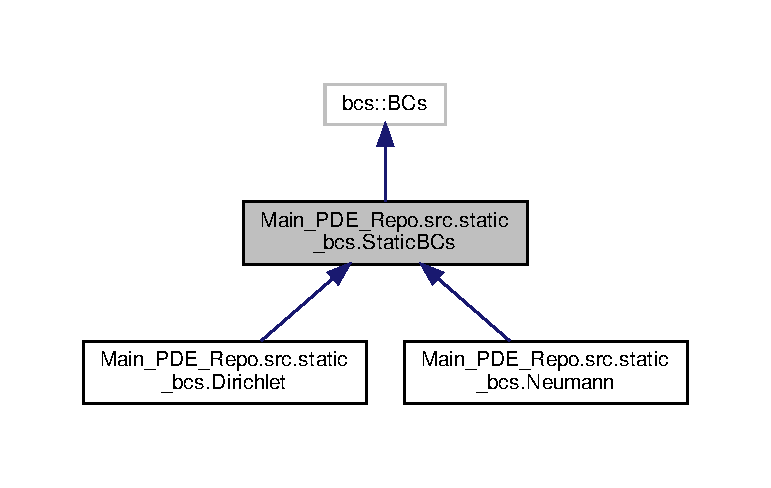
\includegraphics[width=350pt]{classMain__PDE__Repo_1_1src_1_1static__bcs_1_1StaticBCs__inherit__graph}
\end{center}
\end{figure}


Collaboration diagram for Main\+\_\+\+P\+D\+E\+\_\+\+Repo.\+src.\+static\+\_\+bcs.\+Static\+B\+Cs\+:
\nopagebreak
\begin{figure}[H]
\begin{center}
\leavevmode
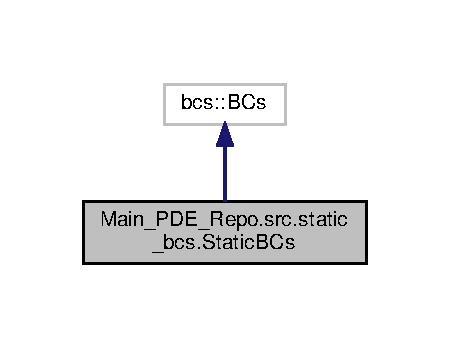
\includegraphics[width=216pt]{classMain__PDE__Repo_1_1src_1_1static__bcs_1_1StaticBCs__coll__graph}
\end{center}
\end{figure}
\subsection*{Public Member Functions}
\begin{DoxyCompactItemize}
\item 
def \hyperlink{classMain__PDE__Repo_1_1src_1_1static__bcs_1_1StaticBCs_a9231c3b0dd3e4263e453d0ba4211dee3}{\+\_\+\+\_\+init\+\_\+\+\_\+} (self, \hyperlink{classMain__PDE__Repo_1_1src_1_1static__bcs_1_1StaticBCs_ad2f589646d3cbb6c43747d26802ca239}{dimen}, \hyperlink{classMain__PDE__Repo_1_1src_1_1static__bcs_1_1StaticBCs_a4f88c825d9bf611f48678b0d606e24e2}{side}, vals)
\begin{DoxyCompactList}\small\item\em The constructor. \end{DoxyCompactList}\item 
def \hyperlink{classMain__PDE__Repo_1_1src_1_1static__bcs_1_1StaticBCs_a46906776d8eb2c4e773b946dd92c4eb8}{print\+\_\+\+B\+Cs} (self)
\begin{DoxyCompactList}\small\item\em Method to spit out the contained boundary conditions, for debugging and planning. \end{DoxyCompactList}\item 
def \hyperlink{classMain__PDE__Repo_1_1src_1_1static__bcs_1_1StaticBCs_a33fc3207e1d39ce2970660ccd31d4084}{get\+\_\+bd} (self)
\begin{DoxyCompactList}\small\item\em Method to return the side that this boundary condition applies to. \end{DoxyCompactList}\item 
def \hyperlink{classMain__PDE__Repo_1_1src_1_1static__bcs_1_1StaticBCs_a12e20f5473740c1a93f3516d64b619fb}{get\+\_\+bcs} (self)
\begin{DoxyCompactList}\small\item\em Method to return the boundary condition values, as a numpy array. \end{DoxyCompactList}\item 
def \hyperlink{classMain__PDE__Repo_1_1src_1_1static__bcs_1_1StaticBCs_a3844f290b44196915bdf036afbcda8a8}{get\+\_\+bctype} (self)
\begin{DoxyCompactList}\small\item\em Method to return the type of boundary condition the object is holding. \end{DoxyCompactList}\end{DoxyCompactItemize}
\subsection*{Public Attributes}
\begin{DoxyCompactItemize}
\item 
\hyperlink{classMain__PDE__Repo_1_1src_1_1static__bcs_1_1StaticBCs_ad2f589646d3cbb6c43747d26802ca239}{dimen}
\item 
\hyperlink{classMain__PDE__Repo_1_1src_1_1static__bcs_1_1StaticBCs_a4f88c825d9bf611f48678b0d606e24e2}{side}
\item 
\hyperlink{classMain__PDE__Repo_1_1src_1_1static__bcs_1_1StaticBCs_a2dfb5aec6e0993299c6c012f6a8b3304}{bound\+\_\+vals}
\end{DoxyCompactItemize}
\subsection*{Static Public Attributes}
\begin{DoxyCompactItemize}
\item 
string \hyperlink{classMain__PDE__Repo_1_1src_1_1static__bcs_1_1StaticBCs_afbdd530a3a47d370c99b30eed8bb0644}{bctype} = \char`\"{}None\char`\"{}
\end{DoxyCompactItemize}


\subsection{Constructor \& Destructor Documentation}
\mbox{\Hypertarget{classMain__PDE__Repo_1_1src_1_1static__bcs_1_1StaticBCs_a9231c3b0dd3e4263e453d0ba4211dee3}\label{classMain__PDE__Repo_1_1src_1_1static__bcs_1_1StaticBCs_a9231c3b0dd3e4263e453d0ba4211dee3}} 
\index{Main\+\_\+\+P\+D\+E\+\_\+\+Repo\+::src\+::static\+\_\+bcs\+::\+Static\+B\+Cs@{Main\+\_\+\+P\+D\+E\+\_\+\+Repo\+::src\+::static\+\_\+bcs\+::\+Static\+B\+Cs}!\+\_\+\+\_\+init\+\_\+\+\_\+@{\+\_\+\+\_\+init\+\_\+\+\_\+}}
\index{\+\_\+\+\_\+init\+\_\+\+\_\+@{\+\_\+\+\_\+init\+\_\+\+\_\+}!Main\+\_\+\+P\+D\+E\+\_\+\+Repo\+::src\+::static\+\_\+bcs\+::\+Static\+B\+Cs@{Main\+\_\+\+P\+D\+E\+\_\+\+Repo\+::src\+::static\+\_\+bcs\+::\+Static\+B\+Cs}}
\subsubsection{\texorpdfstring{\+\_\+\+\_\+init\+\_\+\+\_\+()}{\_\_init\_\_()}}
{\footnotesize\ttfamily def Main\+\_\+\+P\+D\+E\+\_\+\+Repo.\+src.\+static\+\_\+bcs.\+Static\+B\+Cs.\+\_\+\+\_\+init\+\_\+\+\_\+ (\begin{DoxyParamCaption}\item[{}]{self,  }\item[{}]{dimen,  }\item[{}]{side,  }\item[{}]{vals }\end{DoxyParamCaption})}



The constructor. 


\begin{DoxyParams}{Parameters}
{\em dimen} & Int-\/ starting at 0, indicating which dimension the boundary conditions are being applied to. \\
\hline
{\em side} & Char-\/ \textquotesingle{}l\textquotesingle{} or \textquotesingle{}r\textquotesingle{}, the side whose \hyperlink{namespaceMain__PDE__Repo_1_1src_1_1BCs}{B\+Cs} are being represented \\
\hline
{\em vals} & Numpy array-\/ the static values set \\
\hline
\end{DoxyParams}


\subsection{Member Function Documentation}
\mbox{\Hypertarget{classMain__PDE__Repo_1_1src_1_1static__bcs_1_1StaticBCs_a12e20f5473740c1a93f3516d64b619fb}\label{classMain__PDE__Repo_1_1src_1_1static__bcs_1_1StaticBCs_a12e20f5473740c1a93f3516d64b619fb}} 
\index{Main\+\_\+\+P\+D\+E\+\_\+\+Repo\+::src\+::static\+\_\+bcs\+::\+Static\+B\+Cs@{Main\+\_\+\+P\+D\+E\+\_\+\+Repo\+::src\+::static\+\_\+bcs\+::\+Static\+B\+Cs}!get\+\_\+bcs@{get\+\_\+bcs}}
\index{get\+\_\+bcs@{get\+\_\+bcs}!Main\+\_\+\+P\+D\+E\+\_\+\+Repo\+::src\+::static\+\_\+bcs\+::\+Static\+B\+Cs@{Main\+\_\+\+P\+D\+E\+\_\+\+Repo\+::src\+::static\+\_\+bcs\+::\+Static\+B\+Cs}}
\subsubsection{\texorpdfstring{get\+\_\+bcs()}{get\_bcs()}}
{\footnotesize\ttfamily def Main\+\_\+\+P\+D\+E\+\_\+\+Repo.\+src.\+static\+\_\+bcs.\+Static\+B\+Cs.\+get\+\_\+bcs (\begin{DoxyParamCaption}\item[{}]{self }\end{DoxyParamCaption})}



Method to return the boundary condition values, as a numpy array. 

\mbox{\Hypertarget{classMain__PDE__Repo_1_1src_1_1static__bcs_1_1StaticBCs_a3844f290b44196915bdf036afbcda8a8}\label{classMain__PDE__Repo_1_1src_1_1static__bcs_1_1StaticBCs_a3844f290b44196915bdf036afbcda8a8}} 
\index{Main\+\_\+\+P\+D\+E\+\_\+\+Repo\+::src\+::static\+\_\+bcs\+::\+Static\+B\+Cs@{Main\+\_\+\+P\+D\+E\+\_\+\+Repo\+::src\+::static\+\_\+bcs\+::\+Static\+B\+Cs}!get\+\_\+bctype@{get\+\_\+bctype}}
\index{get\+\_\+bctype@{get\+\_\+bctype}!Main\+\_\+\+P\+D\+E\+\_\+\+Repo\+::src\+::static\+\_\+bcs\+::\+Static\+B\+Cs@{Main\+\_\+\+P\+D\+E\+\_\+\+Repo\+::src\+::static\+\_\+bcs\+::\+Static\+B\+Cs}}
\subsubsection{\texorpdfstring{get\+\_\+bctype()}{get\_bctype()}}
{\footnotesize\ttfamily def Main\+\_\+\+P\+D\+E\+\_\+\+Repo.\+src.\+static\+\_\+bcs.\+Static\+B\+Cs.\+get\+\_\+bctype (\begin{DoxyParamCaption}\item[{}]{self }\end{DoxyParamCaption})}



Method to return the type of boundary condition the object is holding. 

\mbox{\Hypertarget{classMain__PDE__Repo_1_1src_1_1static__bcs_1_1StaticBCs_a33fc3207e1d39ce2970660ccd31d4084}\label{classMain__PDE__Repo_1_1src_1_1static__bcs_1_1StaticBCs_a33fc3207e1d39ce2970660ccd31d4084}} 
\index{Main\+\_\+\+P\+D\+E\+\_\+\+Repo\+::src\+::static\+\_\+bcs\+::\+Static\+B\+Cs@{Main\+\_\+\+P\+D\+E\+\_\+\+Repo\+::src\+::static\+\_\+bcs\+::\+Static\+B\+Cs}!get\+\_\+bd@{get\+\_\+bd}}
\index{get\+\_\+bd@{get\+\_\+bd}!Main\+\_\+\+P\+D\+E\+\_\+\+Repo\+::src\+::static\+\_\+bcs\+::\+Static\+B\+Cs@{Main\+\_\+\+P\+D\+E\+\_\+\+Repo\+::src\+::static\+\_\+bcs\+::\+Static\+B\+Cs}}
\subsubsection{\texorpdfstring{get\+\_\+bd()}{get\_bd()}}
{\footnotesize\ttfamily def Main\+\_\+\+P\+D\+E\+\_\+\+Repo.\+src.\+static\+\_\+bcs.\+Static\+B\+Cs.\+get\+\_\+bd (\begin{DoxyParamCaption}\item[{}]{self }\end{DoxyParamCaption})}



Method to return the side that this boundary condition applies to. 

\mbox{\Hypertarget{classMain__PDE__Repo_1_1src_1_1static__bcs_1_1StaticBCs_a46906776d8eb2c4e773b946dd92c4eb8}\label{classMain__PDE__Repo_1_1src_1_1static__bcs_1_1StaticBCs_a46906776d8eb2c4e773b946dd92c4eb8}} 
\index{Main\+\_\+\+P\+D\+E\+\_\+\+Repo\+::src\+::static\+\_\+bcs\+::\+Static\+B\+Cs@{Main\+\_\+\+P\+D\+E\+\_\+\+Repo\+::src\+::static\+\_\+bcs\+::\+Static\+B\+Cs}!print\+\_\+\+B\+Cs@{print\+\_\+\+B\+Cs}}
\index{print\+\_\+\+B\+Cs@{print\+\_\+\+B\+Cs}!Main\+\_\+\+P\+D\+E\+\_\+\+Repo\+::src\+::static\+\_\+bcs\+::\+Static\+B\+Cs@{Main\+\_\+\+P\+D\+E\+\_\+\+Repo\+::src\+::static\+\_\+bcs\+::\+Static\+B\+Cs}}
\subsubsection{\texorpdfstring{print\+\_\+\+B\+Cs()}{print\_BCs()}}
{\footnotesize\ttfamily def Main\+\_\+\+P\+D\+E\+\_\+\+Repo.\+src.\+static\+\_\+bcs.\+Static\+B\+Cs.\+print\+\_\+\+B\+Cs (\begin{DoxyParamCaption}\item[{}]{self }\end{DoxyParamCaption})}



Method to spit out the contained boundary conditions, for debugging and planning. 

Mentions the side number, the kind of boundary, and spits out the prescribed values. 

\subsection{Member Data Documentation}
\mbox{\Hypertarget{classMain__PDE__Repo_1_1src_1_1static__bcs_1_1StaticBCs_afbdd530a3a47d370c99b30eed8bb0644}\label{classMain__PDE__Repo_1_1src_1_1static__bcs_1_1StaticBCs_afbdd530a3a47d370c99b30eed8bb0644}} 
\index{Main\+\_\+\+P\+D\+E\+\_\+\+Repo\+::src\+::static\+\_\+bcs\+::\+Static\+B\+Cs@{Main\+\_\+\+P\+D\+E\+\_\+\+Repo\+::src\+::static\+\_\+bcs\+::\+Static\+B\+Cs}!bctype@{bctype}}
\index{bctype@{bctype}!Main\+\_\+\+P\+D\+E\+\_\+\+Repo\+::src\+::static\+\_\+bcs\+::\+Static\+B\+Cs@{Main\+\_\+\+P\+D\+E\+\_\+\+Repo\+::src\+::static\+\_\+bcs\+::\+Static\+B\+Cs}}
\subsubsection{\texorpdfstring{bctype}{bctype}}
{\footnotesize\ttfamily string Main\+\_\+\+P\+D\+E\+\_\+\+Repo.\+src.\+static\+\_\+bcs.\+Static\+B\+Cs.\+bctype = \char`\"{}None\char`\"{}\hspace{0.3cm}{\ttfamily [static]}}

\mbox{\Hypertarget{classMain__PDE__Repo_1_1src_1_1static__bcs_1_1StaticBCs_a2dfb5aec6e0993299c6c012f6a8b3304}\label{classMain__PDE__Repo_1_1src_1_1static__bcs_1_1StaticBCs_a2dfb5aec6e0993299c6c012f6a8b3304}} 
\index{Main\+\_\+\+P\+D\+E\+\_\+\+Repo\+::src\+::static\+\_\+bcs\+::\+Static\+B\+Cs@{Main\+\_\+\+P\+D\+E\+\_\+\+Repo\+::src\+::static\+\_\+bcs\+::\+Static\+B\+Cs}!bound\+\_\+vals@{bound\+\_\+vals}}
\index{bound\+\_\+vals@{bound\+\_\+vals}!Main\+\_\+\+P\+D\+E\+\_\+\+Repo\+::src\+::static\+\_\+bcs\+::\+Static\+B\+Cs@{Main\+\_\+\+P\+D\+E\+\_\+\+Repo\+::src\+::static\+\_\+bcs\+::\+Static\+B\+Cs}}
\subsubsection{\texorpdfstring{bound\+\_\+vals}{bound\_vals}}
{\footnotesize\ttfamily Main\+\_\+\+P\+D\+E\+\_\+\+Repo.\+src.\+static\+\_\+bcs.\+Static\+B\+Cs.\+bound\+\_\+vals}

\mbox{\Hypertarget{classMain__PDE__Repo_1_1src_1_1static__bcs_1_1StaticBCs_ad2f589646d3cbb6c43747d26802ca239}\label{classMain__PDE__Repo_1_1src_1_1static__bcs_1_1StaticBCs_ad2f589646d3cbb6c43747d26802ca239}} 
\index{Main\+\_\+\+P\+D\+E\+\_\+\+Repo\+::src\+::static\+\_\+bcs\+::\+Static\+B\+Cs@{Main\+\_\+\+P\+D\+E\+\_\+\+Repo\+::src\+::static\+\_\+bcs\+::\+Static\+B\+Cs}!dimen@{dimen}}
\index{dimen@{dimen}!Main\+\_\+\+P\+D\+E\+\_\+\+Repo\+::src\+::static\+\_\+bcs\+::\+Static\+B\+Cs@{Main\+\_\+\+P\+D\+E\+\_\+\+Repo\+::src\+::static\+\_\+bcs\+::\+Static\+B\+Cs}}
\subsubsection{\texorpdfstring{dimen}{dimen}}
{\footnotesize\ttfamily Main\+\_\+\+P\+D\+E\+\_\+\+Repo.\+src.\+static\+\_\+bcs.\+Static\+B\+Cs.\+dimen}

\mbox{\Hypertarget{classMain__PDE__Repo_1_1src_1_1static__bcs_1_1StaticBCs_a4f88c825d9bf611f48678b0d606e24e2}\label{classMain__PDE__Repo_1_1src_1_1static__bcs_1_1StaticBCs_a4f88c825d9bf611f48678b0d606e24e2}} 
\index{Main\+\_\+\+P\+D\+E\+\_\+\+Repo\+::src\+::static\+\_\+bcs\+::\+Static\+B\+Cs@{Main\+\_\+\+P\+D\+E\+\_\+\+Repo\+::src\+::static\+\_\+bcs\+::\+Static\+B\+Cs}!side@{side}}
\index{side@{side}!Main\+\_\+\+P\+D\+E\+\_\+\+Repo\+::src\+::static\+\_\+bcs\+::\+Static\+B\+Cs@{Main\+\_\+\+P\+D\+E\+\_\+\+Repo\+::src\+::static\+\_\+bcs\+::\+Static\+B\+Cs}}
\subsubsection{\texorpdfstring{side}{side}}
{\footnotesize\ttfamily Main\+\_\+\+P\+D\+E\+\_\+\+Repo.\+src.\+static\+\_\+bcs.\+Static\+B\+Cs.\+side}



The documentation for this class was generated from the following file\+:\begin{DoxyCompactItemize}
\item 
src/\hyperlink{static__bcs_8py}{static\+\_\+bcs.\+py}\end{DoxyCompactItemize}

\hypertarget{classMain__PDE__Repo_1_1src_1_1stencil_1_1Stencil}{}\section{Main\+\_\+\+P\+D\+E\+\_\+\+Repo.\+src.\+stencil.\+Stencil Class Reference}
\label{classMain__PDE__Repo_1_1src_1_1stencil_1_1Stencil}\index{Main\+\_\+\+P\+D\+E\+\_\+\+Repo.\+src.\+stencil.\+Stencil@{Main\+\_\+\+P\+D\+E\+\_\+\+Repo.\+src.\+stencil.\+Stencil}}


\hyperlink{classMain__PDE__Repo_1_1src_1_1stencil_1_1Stencil}{Stencil} A finite difference stencil to calculate an operator.  


\subsection*{Public Member Functions}
\begin{DoxyCompactItemize}
\item 
def \hyperlink{classMain__PDE__Repo_1_1src_1_1stencil_1_1Stencil_ac28834812ca6c6afcaf499809a8f6c57}{\+\_\+\+\_\+init\+\_\+\+\_\+} (self, \hyperlink{classMain__PDE__Repo_1_1src_1_1stencil_1_1Stencil_a8522227e34c5d0d63a988ccf1d589fd9}{s})
\item 
def \hyperlink{classMain__PDE__Repo_1_1src_1_1stencil_1_1Stencil_a929a771df412bf27d03c2aae1a4ee7a0}{get\+\_\+weights} (self, d)
\end{DoxyCompactItemize}
\subsection*{Public Attributes}
\begin{DoxyCompactItemize}
\item 
\hyperlink{classMain__PDE__Repo_1_1src_1_1stencil_1_1Stencil_a8522227e34c5d0d63a988ccf1d589fd9}{s}
\item 
\hyperlink{classMain__PDE__Repo_1_1src_1_1stencil_1_1Stencil_a23797c4ec3adad5ab929cc221de8d7f7}{N}
\item 
\hyperlink{classMain__PDE__Repo_1_1src_1_1stencil_1_1Stencil_a008c7722934b3af3a21d8d945f12b597}{s\+\_\+matrix}
\end{DoxyCompactItemize}
\subsection*{Private Member Functions}
\begin{DoxyCompactItemize}
\item 
def \hyperlink{classMain__PDE__Repo_1_1src_1_1stencil_1_1Stencil_a785c9ea7126ed706d574907d114ccf57}{\+\_\+stencil\+\_\+matrix} (self)
\end{DoxyCompactItemize}


\subsection{Detailed Description}
\hyperlink{classMain__PDE__Repo_1_1src_1_1stencil_1_1Stencil}{Stencil} A finite difference stencil to calculate an operator. 



\subsection{Constructor \& Destructor Documentation}
\mbox{\Hypertarget{classMain__PDE__Repo_1_1src_1_1stencil_1_1Stencil_ac28834812ca6c6afcaf499809a8f6c57}\label{classMain__PDE__Repo_1_1src_1_1stencil_1_1Stencil_ac28834812ca6c6afcaf499809a8f6c57}} 
\index{Main\+\_\+\+P\+D\+E\+\_\+\+Repo\+::src\+::stencil\+::\+Stencil@{Main\+\_\+\+P\+D\+E\+\_\+\+Repo\+::src\+::stencil\+::\+Stencil}!\+\_\+\+\_\+init\+\_\+\+\_\+@{\+\_\+\+\_\+init\+\_\+\+\_\+}}
\index{\+\_\+\+\_\+init\+\_\+\+\_\+@{\+\_\+\+\_\+init\+\_\+\+\_\+}!Main\+\_\+\+P\+D\+E\+\_\+\+Repo\+::src\+::stencil\+::\+Stencil@{Main\+\_\+\+P\+D\+E\+\_\+\+Repo\+::src\+::stencil\+::\+Stencil}}
\subsubsection{\texorpdfstring{\+\_\+\+\_\+init\+\_\+\+\_\+()}{\_\_init\_\_()}}
{\footnotesize\ttfamily def Main\+\_\+\+P\+D\+E\+\_\+\+Repo.\+src.\+stencil.\+Stencil.\+\_\+\+\_\+init\+\_\+\+\_\+ (\begin{DoxyParamCaption}\item[{}]{self,  }\item[{}]{s }\end{DoxyParamCaption})}



\subsection{Member Function Documentation}
\mbox{\Hypertarget{classMain__PDE__Repo_1_1src_1_1stencil_1_1Stencil_a785c9ea7126ed706d574907d114ccf57}\label{classMain__PDE__Repo_1_1src_1_1stencil_1_1Stencil_a785c9ea7126ed706d574907d114ccf57}} 
\index{Main\+\_\+\+P\+D\+E\+\_\+\+Repo\+::src\+::stencil\+::\+Stencil@{Main\+\_\+\+P\+D\+E\+\_\+\+Repo\+::src\+::stencil\+::\+Stencil}!\+\_\+stencil\+\_\+matrix@{\+\_\+stencil\+\_\+matrix}}
\index{\+\_\+stencil\+\_\+matrix@{\+\_\+stencil\+\_\+matrix}!Main\+\_\+\+P\+D\+E\+\_\+\+Repo\+::src\+::stencil\+::\+Stencil@{Main\+\_\+\+P\+D\+E\+\_\+\+Repo\+::src\+::stencil\+::\+Stencil}}
\subsubsection{\texorpdfstring{\+\_\+stencil\+\_\+matrix()}{\_stencil\_matrix()}}
{\footnotesize\ttfamily def Main\+\_\+\+P\+D\+E\+\_\+\+Repo.\+src.\+stencil.\+Stencil.\+\_\+stencil\+\_\+matrix (\begin{DoxyParamCaption}\item[{}]{self }\end{DoxyParamCaption})\hspace{0.3cm}{\ttfamily [private]}}

\mbox{\Hypertarget{classMain__PDE__Repo_1_1src_1_1stencil_1_1Stencil_a929a771df412bf27d03c2aae1a4ee7a0}\label{classMain__PDE__Repo_1_1src_1_1stencil_1_1Stencil_a929a771df412bf27d03c2aae1a4ee7a0}} 
\index{Main\+\_\+\+P\+D\+E\+\_\+\+Repo\+::src\+::stencil\+::\+Stencil@{Main\+\_\+\+P\+D\+E\+\_\+\+Repo\+::src\+::stencil\+::\+Stencil}!get\+\_\+weights@{get\+\_\+weights}}
\index{get\+\_\+weights@{get\+\_\+weights}!Main\+\_\+\+P\+D\+E\+\_\+\+Repo\+::src\+::stencil\+::\+Stencil@{Main\+\_\+\+P\+D\+E\+\_\+\+Repo\+::src\+::stencil\+::\+Stencil}}
\subsubsection{\texorpdfstring{get\+\_\+weights()}{get\_weights()}}
{\footnotesize\ttfamily def Main\+\_\+\+P\+D\+E\+\_\+\+Repo.\+src.\+stencil.\+Stencil.\+get\+\_\+weights (\begin{DoxyParamCaption}\item[{}]{self,  }\item[{}]{d }\end{DoxyParamCaption})}



\subsection{Member Data Documentation}
\mbox{\Hypertarget{classMain__PDE__Repo_1_1src_1_1stencil_1_1Stencil_a23797c4ec3adad5ab929cc221de8d7f7}\label{classMain__PDE__Repo_1_1src_1_1stencil_1_1Stencil_a23797c4ec3adad5ab929cc221de8d7f7}} 
\index{Main\+\_\+\+P\+D\+E\+\_\+\+Repo\+::src\+::stencil\+::\+Stencil@{Main\+\_\+\+P\+D\+E\+\_\+\+Repo\+::src\+::stencil\+::\+Stencil}!N@{N}}
\index{N@{N}!Main\+\_\+\+P\+D\+E\+\_\+\+Repo\+::src\+::stencil\+::\+Stencil@{Main\+\_\+\+P\+D\+E\+\_\+\+Repo\+::src\+::stencil\+::\+Stencil}}
\subsubsection{\texorpdfstring{N}{N}}
{\footnotesize\ttfamily Main\+\_\+\+P\+D\+E\+\_\+\+Repo.\+src.\+stencil.\+Stencil.\+N}

\mbox{\Hypertarget{classMain__PDE__Repo_1_1src_1_1stencil_1_1Stencil_a8522227e34c5d0d63a988ccf1d589fd9}\label{classMain__PDE__Repo_1_1src_1_1stencil_1_1Stencil_a8522227e34c5d0d63a988ccf1d589fd9}} 
\index{Main\+\_\+\+P\+D\+E\+\_\+\+Repo\+::src\+::stencil\+::\+Stencil@{Main\+\_\+\+P\+D\+E\+\_\+\+Repo\+::src\+::stencil\+::\+Stencil}!s@{s}}
\index{s@{s}!Main\+\_\+\+P\+D\+E\+\_\+\+Repo\+::src\+::stencil\+::\+Stencil@{Main\+\_\+\+P\+D\+E\+\_\+\+Repo\+::src\+::stencil\+::\+Stencil}}
\subsubsection{\texorpdfstring{s}{s}}
{\footnotesize\ttfamily Main\+\_\+\+P\+D\+E\+\_\+\+Repo.\+src.\+stencil.\+Stencil.\+s}

\mbox{\Hypertarget{classMain__PDE__Repo_1_1src_1_1stencil_1_1Stencil_a008c7722934b3af3a21d8d945f12b597}\label{classMain__PDE__Repo_1_1src_1_1stencil_1_1Stencil_a008c7722934b3af3a21d8d945f12b597}} 
\index{Main\+\_\+\+P\+D\+E\+\_\+\+Repo\+::src\+::stencil\+::\+Stencil@{Main\+\_\+\+P\+D\+E\+\_\+\+Repo\+::src\+::stencil\+::\+Stencil}!s\+\_\+matrix@{s\+\_\+matrix}}
\index{s\+\_\+matrix@{s\+\_\+matrix}!Main\+\_\+\+P\+D\+E\+\_\+\+Repo\+::src\+::stencil\+::\+Stencil@{Main\+\_\+\+P\+D\+E\+\_\+\+Repo\+::src\+::stencil\+::\+Stencil}}
\subsubsection{\texorpdfstring{s\+\_\+matrix}{s\_matrix}}
{\footnotesize\ttfamily Main\+\_\+\+P\+D\+E\+\_\+\+Repo.\+src.\+stencil.\+Stencil.\+s\+\_\+matrix}



The documentation for this class was generated from the following file\+:\begin{DoxyCompactItemize}
\item 
src/\hyperlink{stencil_8py}{stencil.\+py}\end{DoxyCompactItemize}

\hypertarget{classMain__PDE__Repo_1_1src_1_1time__stepper_1_1TimeStepper}{}\section{Main\+\_\+\+P\+D\+E\+\_\+\+Repo.\+src.\+time\+\_\+stepper.\+Time\+Stepper Class Reference}
\label{classMain__PDE__Repo_1_1src_1_1time__stepper_1_1TimeStepper}\index{Main\+\_\+\+P\+D\+E\+\_\+\+Repo.\+src.\+time\+\_\+stepper.\+Time\+Stepper@{Main\+\_\+\+P\+D\+E\+\_\+\+Repo.\+src.\+time\+\_\+stepper.\+Time\+Stepper}}


The abstract \hyperlink{classMain__PDE__Repo_1_1src_1_1time__stepper_1_1TimeStepper}{Time\+Stepper} class.  




Inheritance diagram for Main\+\_\+\+P\+D\+E\+\_\+\+Repo.\+src.\+time\+\_\+stepper.\+Time\+Stepper\+:
\nopagebreak
\begin{figure}[H]
\begin{center}
\leavevmode
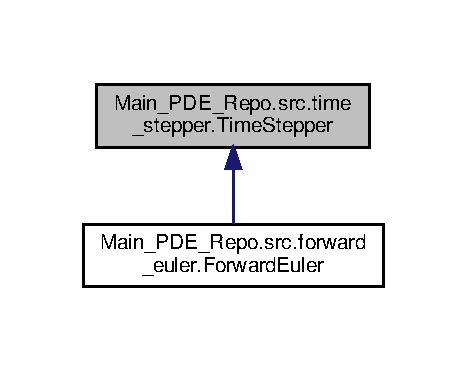
\includegraphics[width=224pt]{classMain__PDE__Repo_1_1src_1_1time__stepper_1_1TimeStepper__inherit__graph}
\end{center}
\end{figure}
\subsection*{Public Member Functions}
\begin{DoxyCompactItemize}
\item 
def \hyperlink{classMain__PDE__Repo_1_1src_1_1time__stepper_1_1TimeStepper_a4e5f0ba51d77777a3ef499258f1982ac}{step} (self, val\+\_\+grid, rhs\+\_\+grid, dt)
\begin{DoxyCompactList}\small\item\em The main step method of the time stepper. \end{DoxyCompactList}\end{DoxyCompactItemize}


\subsection{Detailed Description}
The abstract \hyperlink{classMain__PDE__Repo_1_1src_1_1time__stepper_1_1TimeStepper}{Time\+Stepper} class. 

\subsection{Member Function Documentation}
\mbox{\Hypertarget{classMain__PDE__Repo_1_1src_1_1time__stepper_1_1TimeStepper_a4e5f0ba51d77777a3ef499258f1982ac}\label{classMain__PDE__Repo_1_1src_1_1time__stepper_1_1TimeStepper_a4e5f0ba51d77777a3ef499258f1982ac}} 
\index{Main\+\_\+\+P\+D\+E\+\_\+\+Repo\+::src\+::time\+\_\+stepper\+::\+Time\+Stepper@{Main\+\_\+\+P\+D\+E\+\_\+\+Repo\+::src\+::time\+\_\+stepper\+::\+Time\+Stepper}!step@{step}}
\index{step@{step}!Main\+\_\+\+P\+D\+E\+\_\+\+Repo\+::src\+::time\+\_\+stepper\+::\+Time\+Stepper@{Main\+\_\+\+P\+D\+E\+\_\+\+Repo\+::src\+::time\+\_\+stepper\+::\+Time\+Stepper}}
\subsubsection{\texorpdfstring{step()}{step()}}
{\footnotesize\ttfamily def Main\+\_\+\+P\+D\+E\+\_\+\+Repo.\+src.\+time\+\_\+stepper.\+Time\+Stepper.\+step (\begin{DoxyParamCaption}\item[{}]{self,  }\item[{}]{val\+\_\+grid,  }\item[{}]{rhs\+\_\+grid,  }\item[{}]{dt }\end{DoxyParamCaption})}



The main step method of the time stepper. 

This method must be overwritten in the child class where the actual implementation algorithm is defined. 
\begin{DoxyParams}{Parameters}
{\em val\+\_\+grid} & The spatial grid of values at the current time \\
\hline
{\em rhs\+\_\+grid} & The spatial grid of R\+HS values \\
\hline
{\em dt} & The time step size \\
\hline
\end{DoxyParams}
\begin{DoxyReturn}{Returns}
Spatial grid with new values for the next time step 
\end{DoxyReturn}


The documentation for this class was generated from the following file\+:\begin{DoxyCompactItemize}
\item 
src/\hyperlink{time__stepper_8py}{time\+\_\+stepper.\+py}\end{DoxyCompactItemize}

\hypertarget{classMain__PDE__Repo_1_1src_1_1vis__gif__2d_1_1VisGif2d}{}\section{Main\+\_\+\+P\+D\+E\+\_\+\+Repo.\+src.\+vis\+\_\+gif\+\_\+2d.\+Vis\+Gif2d Class Reference}
\label{classMain__PDE__Repo_1_1src_1_1vis__gif__2d_1_1VisGif2d}\index{Main\+\_\+\+P\+D\+E\+\_\+\+Repo.\+src.\+vis\+\_\+gif\+\_\+2d.\+Vis\+Gif2d@{Main\+\_\+\+P\+D\+E\+\_\+\+Repo.\+src.\+vis\+\_\+gif\+\_\+2d.\+Vis\+Gif2d}}


Class for creating a gif movie of simulation results for 2d scalar variables.  




Inheritance diagram for Main\+\_\+\+P\+D\+E\+\_\+\+Repo.\+src.\+vis\+\_\+gif\+\_\+2d.\+Vis\+Gif2d\+:
\nopagebreak
\begin{figure}[H]
\begin{center}
\leavevmode
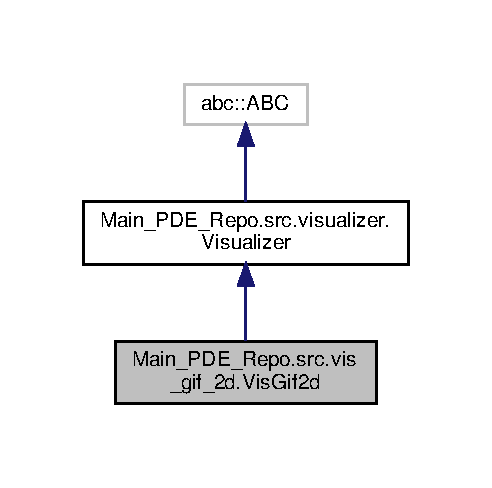
\includegraphics[width=236pt]{classMain__PDE__Repo_1_1src_1_1vis__gif__2d_1_1VisGif2d__inherit__graph}
\end{center}
\end{figure}


Collaboration diagram for Main\+\_\+\+P\+D\+E\+\_\+\+Repo.\+src.\+vis\+\_\+gif\+\_\+2d.\+Vis\+Gif2d\+:
\nopagebreak
\begin{figure}[H]
\begin{center}
\leavevmode
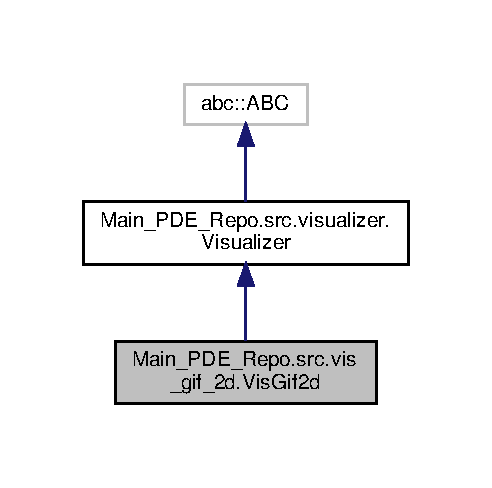
\includegraphics[width=236pt]{classMain__PDE__Repo_1_1src_1_1vis__gif__2d_1_1VisGif2d__coll__graph}
\end{center}
\end{figure}
\subsection*{Public Member Functions}
\begin{DoxyCompactItemize}
\item 
def \hyperlink{classMain__PDE__Repo_1_1src_1_1vis__gif__2d_1_1VisGif2d_ac831ff56d31525f11311e5b6e4c894a6}{\+\_\+\+\_\+init\+\_\+\+\_\+} (self, \hyperlink{classMain__PDE__Repo_1_1src_1_1vis__gif__2d_1_1VisGif2d_a48a438a24012dc8496b8008ab4f13da0}{direc})
\begin{DoxyCompactList}\small\item\em The constructor. \end{DoxyCompactList}\item 
def \hyperlink{classMain__PDE__Repo_1_1src_1_1vis__gif__2d_1_1VisGif2d_aa4b0092b49e7fecbc62f57adcd491c12}{make\+\_\+2d\+\_\+movie} (self, log, name=\char`\"{}\char`\"{}, kwargs)
\begin{DoxyCompactList}\small\item\em Generates a 2d movie of the output from logger and saves it as a G\+IF to the given output directory. \end{DoxyCompactList}\end{DoxyCompactItemize}
\subsection*{Public Attributes}
\begin{DoxyCompactItemize}
\item 
\hyperlink{classMain__PDE__Repo_1_1src_1_1vis__gif__2d_1_1VisGif2d_a48a438a24012dc8496b8008ab4f13da0}{direc}
\end{DoxyCompactItemize}
\subsection*{Private Member Functions}
\begin{DoxyCompactItemize}
\item 
def \hyperlink{classMain__PDE__Repo_1_1src_1_1vis__gif__2d_1_1VisGif2d_abf86f9c00a0481f04e982efbea8520ed}{\+\_\+animate} (self, i, X, Y, ax, surf, log)
\begin{DoxyCompactList}\small\item\em Method used to step forward a frame for the make\+\_\+2d\+\_\+movie method. \end{DoxyCompactList}\end{DoxyCompactItemize}


\subsection{Detailed Description}
Class for creating a gif movie of simulation results for 2d scalar variables. 

\subsection{Constructor \& Destructor Documentation}
\mbox{\Hypertarget{classMain__PDE__Repo_1_1src_1_1vis__gif__2d_1_1VisGif2d_ac831ff56d31525f11311e5b6e4c894a6}\label{classMain__PDE__Repo_1_1src_1_1vis__gif__2d_1_1VisGif2d_ac831ff56d31525f11311e5b6e4c894a6}} 
\index{Main\+\_\+\+P\+D\+E\+\_\+\+Repo\+::src\+::vis\+\_\+gif\+\_\+2d\+::\+Vis\+Gif2d@{Main\+\_\+\+P\+D\+E\+\_\+\+Repo\+::src\+::vis\+\_\+gif\+\_\+2d\+::\+Vis\+Gif2d}!\+\_\+\+\_\+init\+\_\+\+\_\+@{\+\_\+\+\_\+init\+\_\+\+\_\+}}
\index{\+\_\+\+\_\+init\+\_\+\+\_\+@{\+\_\+\+\_\+init\+\_\+\+\_\+}!Main\+\_\+\+P\+D\+E\+\_\+\+Repo\+::src\+::vis\+\_\+gif\+\_\+2d\+::\+Vis\+Gif2d@{Main\+\_\+\+P\+D\+E\+\_\+\+Repo\+::src\+::vis\+\_\+gif\+\_\+2d\+::\+Vis\+Gif2d}}
\subsubsection{\texorpdfstring{\+\_\+\+\_\+init\+\_\+\+\_\+()}{\_\_init\_\_()}}
{\footnotesize\ttfamily def Main\+\_\+\+P\+D\+E\+\_\+\+Repo.\+src.\+vis\+\_\+gif\+\_\+2d.\+Vis\+Gif2d.\+\_\+\+\_\+init\+\_\+\+\_\+ (\begin{DoxyParamCaption}\item[{}]{self,  }\item[{}]{direc }\end{DoxyParamCaption})}



The constructor. 

\hyperlink{classMain__PDE__Repo_1_1src_1_1vis__gif__2d_1_1VisGif2d}{Vis\+Gif2d} objects are instantiated with an output directory. 
\begin{DoxyParams}{Parameters}
{\em direc} & The directory in which to save the output \\
\hline
\end{DoxyParams}


\subsection{Member Function Documentation}
\mbox{\Hypertarget{classMain__PDE__Repo_1_1src_1_1vis__gif__2d_1_1VisGif2d_abf86f9c00a0481f04e982efbea8520ed}\label{classMain__PDE__Repo_1_1src_1_1vis__gif__2d_1_1VisGif2d_abf86f9c00a0481f04e982efbea8520ed}} 
\index{Main\+\_\+\+P\+D\+E\+\_\+\+Repo\+::src\+::vis\+\_\+gif\+\_\+2d\+::\+Vis\+Gif2d@{Main\+\_\+\+P\+D\+E\+\_\+\+Repo\+::src\+::vis\+\_\+gif\+\_\+2d\+::\+Vis\+Gif2d}!\+\_\+animate@{\+\_\+animate}}
\index{\+\_\+animate@{\+\_\+animate}!Main\+\_\+\+P\+D\+E\+\_\+\+Repo\+::src\+::vis\+\_\+gif\+\_\+2d\+::\+Vis\+Gif2d@{Main\+\_\+\+P\+D\+E\+\_\+\+Repo\+::src\+::vis\+\_\+gif\+\_\+2d\+::\+Vis\+Gif2d}}
\subsubsection{\texorpdfstring{\+\_\+animate()}{\_animate()}}
{\footnotesize\ttfamily def Main\+\_\+\+P\+D\+E\+\_\+\+Repo.\+src.\+vis\+\_\+gif\+\_\+2d.\+Vis\+Gif2d.\+\_\+animate (\begin{DoxyParamCaption}\item[{}]{self,  }\item[{}]{i,  }\item[{}]{X,  }\item[{}]{Y,  }\item[{}]{ax,  }\item[{}]{surf,  }\item[{}]{log }\end{DoxyParamCaption})\hspace{0.3cm}{\ttfamily [private]}}



Method used to step forward a frame for the make\+\_\+2d\+\_\+movie method. 


\begin{DoxyParams}{Parameters}
{\em i} & The frame to step to \\
\hline
{\em X} & The dim number 0 meshgrid \\
\hline
{\em Y} & The dim number 1 meshgrid \\
\hline
{\em ax} & The matplotlib Axes object used to make the ovie \\
\hline
{\em surf} & The matplotlib ax.\+plot\+\_\+surface() instance to update \\
\hline
{\em log} & The Logger object containing the data to be plotted \\
\hline
\end{DoxyParams}
\mbox{\Hypertarget{classMain__PDE__Repo_1_1src_1_1vis__gif__2d_1_1VisGif2d_aa4b0092b49e7fecbc62f57adcd491c12}\label{classMain__PDE__Repo_1_1src_1_1vis__gif__2d_1_1VisGif2d_aa4b0092b49e7fecbc62f57adcd491c12}} 
\index{Main\+\_\+\+P\+D\+E\+\_\+\+Repo\+::src\+::vis\+\_\+gif\+\_\+2d\+::\+Vis\+Gif2d@{Main\+\_\+\+P\+D\+E\+\_\+\+Repo\+::src\+::vis\+\_\+gif\+\_\+2d\+::\+Vis\+Gif2d}!make\+\_\+2d\+\_\+movie@{make\+\_\+2d\+\_\+movie}}
\index{make\+\_\+2d\+\_\+movie@{make\+\_\+2d\+\_\+movie}!Main\+\_\+\+P\+D\+E\+\_\+\+Repo\+::src\+::vis\+\_\+gif\+\_\+2d\+::\+Vis\+Gif2d@{Main\+\_\+\+P\+D\+E\+\_\+\+Repo\+::src\+::vis\+\_\+gif\+\_\+2d\+::\+Vis\+Gif2d}}
\subsubsection{\texorpdfstring{make\+\_\+2d\+\_\+movie()}{make\_2d\_movie()}}
{\footnotesize\ttfamily def Main\+\_\+\+P\+D\+E\+\_\+\+Repo.\+src.\+vis\+\_\+gif\+\_\+2d.\+Vis\+Gif2d.\+make\+\_\+2d\+\_\+movie (\begin{DoxyParamCaption}\item[{}]{self,  }\item[{}]{log,  }\item[{}]{name = {\ttfamily \char`\"{}\char`\"{}},  }\item[{}]{kwargs }\end{DoxyParamCaption})}



Generates a 2d movie of the output from logger and saves it as a G\+IF to the given output directory. 


\begin{DoxyParams}{Parameters}
{\em log} & The Logger object containing the data to be animated. \\
\hline
\end{DoxyParams}


\subsection{Member Data Documentation}
\mbox{\Hypertarget{classMain__PDE__Repo_1_1src_1_1vis__gif__2d_1_1VisGif2d_a48a438a24012dc8496b8008ab4f13da0}\label{classMain__PDE__Repo_1_1src_1_1vis__gif__2d_1_1VisGif2d_a48a438a24012dc8496b8008ab4f13da0}} 
\index{Main\+\_\+\+P\+D\+E\+\_\+\+Repo\+::src\+::vis\+\_\+gif\+\_\+2d\+::\+Vis\+Gif2d@{Main\+\_\+\+P\+D\+E\+\_\+\+Repo\+::src\+::vis\+\_\+gif\+\_\+2d\+::\+Vis\+Gif2d}!direc@{direc}}
\index{direc@{direc}!Main\+\_\+\+P\+D\+E\+\_\+\+Repo\+::src\+::vis\+\_\+gif\+\_\+2d\+::\+Vis\+Gif2d@{Main\+\_\+\+P\+D\+E\+\_\+\+Repo\+::src\+::vis\+\_\+gif\+\_\+2d\+::\+Vis\+Gif2d}}
\subsubsection{\texorpdfstring{direc}{direc}}
{\footnotesize\ttfamily Main\+\_\+\+P\+D\+E\+\_\+\+Repo.\+src.\+vis\+\_\+gif\+\_\+2d.\+Vis\+Gif2d.\+direc}



The documentation for this class was generated from the following file\+:\begin{DoxyCompactItemize}
\item 
src/\hyperlink{vis__gif__2d_8py}{vis\+\_\+gif\+\_\+2d.\+py}\end{DoxyCompactItemize}

\hypertarget{classMain__PDE__Repo_1_1src_1_1visualizer_1_1Visualizer}{}\section{Main\+\_\+\+P\+D\+E\+\_\+\+Repo.\+src.\+visualizer.\+Visualizer Class Reference}
\label{classMain__PDE__Repo_1_1src_1_1visualizer_1_1Visualizer}\index{Main\+\_\+\+P\+D\+E\+\_\+\+Repo.\+src.\+visualizer.\+Visualizer@{Main\+\_\+\+P\+D\+E\+\_\+\+Repo.\+src.\+visualizer.\+Visualizer}}


The \hyperlink{classMain__PDE__Repo_1_1src_1_1visualizer_1_1Visualizer}{Visualizer} abstract baseclass Nothing is in it right now, but other classes could potentially inherit things from it.  




Inheritance diagram for Main\+\_\+\+P\+D\+E\+\_\+\+Repo.\+src.\+visualizer.\+Visualizer\+:
\nopagebreak
\begin{figure}[H]
\begin{center}
\leavevmode
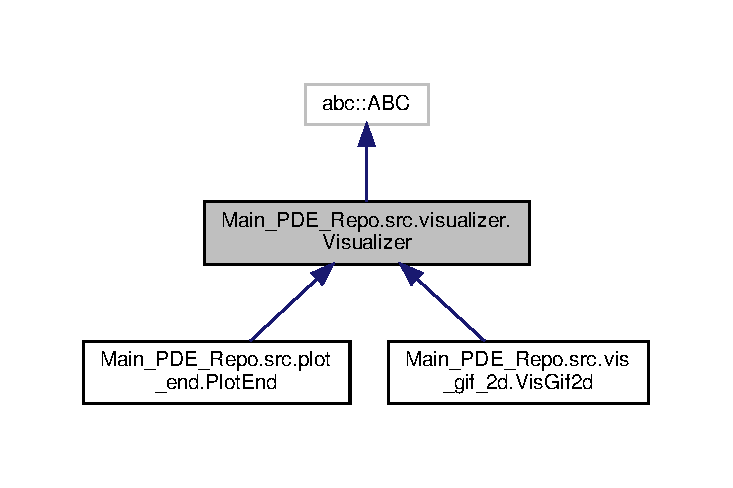
\includegraphics[width=350pt]{classMain__PDE__Repo_1_1src_1_1visualizer_1_1Visualizer__inherit__graph}
\end{center}
\end{figure}


Collaboration diagram for Main\+\_\+\+P\+D\+E\+\_\+\+Repo.\+src.\+visualizer.\+Visualizer\+:
\nopagebreak
\begin{figure}[H]
\begin{center}
\leavevmode
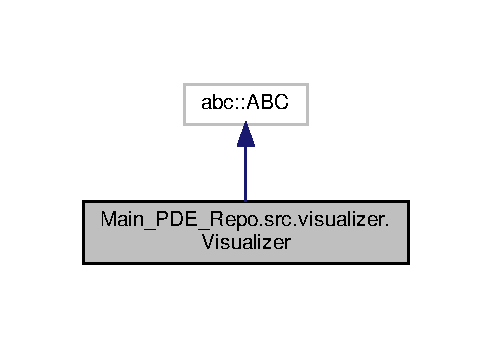
\includegraphics[width=236pt]{classMain__PDE__Repo_1_1src_1_1visualizer_1_1Visualizer__coll__graph}
\end{center}
\end{figure}


\subsection{Detailed Description}
The \hyperlink{classMain__PDE__Repo_1_1src_1_1visualizer_1_1Visualizer}{Visualizer} abstract baseclass Nothing is in it right now, but other classes could potentially inherit things from it. 

The documentation for this class was generated from the following file\+:\begin{DoxyCompactItemize}
\item 
src/\hyperlink{visualizer_8py}{visualizer.\+py}\end{DoxyCompactItemize}

\chapter{File Documentation}
\hypertarget{____init_____8py}{}\section{\+\_\+\+\_\+init\+\_\+\+\_\+.\+py File Reference}
\label{____init_____8py}\index{\+\_\+\+\_\+init\+\_\+\+\_\+.\+py@{\+\_\+\+\_\+init\+\_\+\+\_\+.\+py}}
\subsection*{Namespaces}
\begin{DoxyCompactItemize}
\item 
 \hyperlink{namespaceMain__PDE__Repo}{Main\+\_\+\+P\+D\+E\+\_\+\+Repo}
\end{DoxyCompactItemize}

\hypertarget{src_2____init_____8py}{}\section{src/\+\_\+\+\_\+init\+\_\+\+\_\+.py File Reference}
\label{src_2____init_____8py}\index{src/\+\_\+\+\_\+init\+\_\+\+\_\+.\+py@{src/\+\_\+\+\_\+init\+\_\+\+\_\+.\+py}}
\subsection*{Namespaces}
\begin{DoxyCompactItemize}
\item 
 \hyperlink{namespaceMain__PDE__Repo_1_1src}{Main\+\_\+\+P\+D\+E\+\_\+\+Repo.\+src}
\end{DoxyCompactItemize}

\hypertarget{initializer_8py}{}\section{initializer.\+py File Reference}
\label{initializer_8py}\index{initializer.\+py@{initializer.\+py}}
\subsection*{Namespaces}
\begin{DoxyCompactItemize}
\item 
 \hyperlink{namespaceMain__PDE__Repo_1_1initializer}{Main\+\_\+\+P\+D\+E\+\_\+\+Repo.\+initializer}
\end{DoxyCompactItemize}
\subsection*{Variables}
\begin{DoxyCompactItemize}
\item 
string \hyperlink{namespaceMain__PDE__Repo_1_1initializer_acf6a435968a90051222f233d914c5397}{Main\+\_\+\+P\+D\+E\+\_\+\+Repo.\+initializer.\+out\+\_\+loc} = r\char`\"{}outputs/\char`\"{}
\item 
string \hyperlink{namespaceMain__PDE__Repo_1_1initializer_a46b587e3a760d2bc366f1b38609c5af9}{Main\+\_\+\+P\+D\+E\+\_\+\+Repo.\+initializer.\+out\+\_\+name} = \char`\"{}initializer\+\_\+2d\+\_\+plot\+\_\+3\char`\"{}
\item 
float \hyperlink{namespaceMain__PDE__Repo_1_1initializer_a8f26c89cc507005999c925cc575638cf}{Main\+\_\+\+P\+D\+E\+\_\+\+Repo.\+initializer.\+t\+\_\+start} = 0.\+0
\item 
float \hyperlink{namespaceMain__PDE__Repo_1_1initializer_ab123ebb4c5c95ab09b8d8310af223730}{Main\+\_\+\+P\+D\+E\+\_\+\+Repo.\+initializer.\+t\+\_\+end} = 2.\+0
\item 
float \hyperlink{namespaceMain__PDE__Repo_1_1initializer_ab8ea6f49ea65c76cfaa727f10e349ec5}{Main\+\_\+\+P\+D\+E\+\_\+\+Repo.\+initializer.\+dt} = 0.\+0001
\item 
int \hyperlink{namespaceMain__PDE__Repo_1_1initializer_a7b9a1175cb86388f7315a7c6dee797e3}{Main\+\_\+\+P\+D\+E\+\_\+\+Repo.\+initializer.\+nx} = 100
\item 
int \hyperlink{namespaceMain__PDE__Repo_1_1initializer_a705f203425c609ebc41db74879bf413a}{Main\+\_\+\+P\+D\+E\+\_\+\+Repo.\+initializer.\+ny} = 100
\item 
int \hyperlink{namespaceMain__PDE__Repo_1_1initializer_ab7752e585cb1e9951e583722826dc47b}{Main\+\_\+\+P\+D\+E\+\_\+\+Repo.\+initializer.\+dx} = 2 / (nx -\/ 1)
\item 
int \hyperlink{namespaceMain__PDE__Repo_1_1initializer_aa755829a50d6b513279ec4ac18abd4ba}{Main\+\_\+\+P\+D\+E\+\_\+\+Repo.\+initializer.\+dy} = 2 / (ny -\/ 1)
\item 
\hyperlink{namespaceMain__PDE__Repo_1_1initializer_a495f211daae2ee5ae3bbdb86436c35b5}{Main\+\_\+\+P\+D\+E\+\_\+\+Repo.\+initializer.\+x} = np.\+linspace(0, 2, nx)
\item 
\hyperlink{namespaceMain__PDE__Repo_1_1initializer_a0963e63e11418e26d8cc428b47669ff1}{Main\+\_\+\+P\+D\+E\+\_\+\+Repo.\+initializer.\+y} = np.\+linspace(0, 2, ny)
\item 
tuple \hyperlink{namespaceMain__PDE__Repo_1_1initializer_a3349742a76f7fa24317809e551e4b27a}{Main\+\_\+\+P\+D\+E\+\_\+\+Repo.\+initializer.\+coords} = (tuple(y),tuple(x))
\item 
\hyperlink{namespaceMain__PDE__Repo_1_1initializer_af0ec17a2fbde89969e4c442f9f4fda75}{Main\+\_\+\+P\+D\+E\+\_\+\+Repo.\+initializer.\+u} = np.\+zeros((ny,nx))
\item 
\hyperlink{namespaceMain__PDE__Repo_1_1initializer_a657e8b73e6463b4e45e67b4854e3bdcc}{Main\+\_\+\+P\+D\+E\+\_\+\+Repo.\+initializer.\+d2\+\_\+int} = operator\+\_\+1d.\+Operator1D(\mbox{[}-\/1,0,1\mbox{]}, 2)
\item 
\hyperlink{namespaceMain__PDE__Repo_1_1initializer_a588f8a108166ccbf39c9e31dd69a1a7c}{Main\+\_\+\+P\+D\+E\+\_\+\+Repo.\+initializer.\+laplac\+\_\+int} = operator\+\_\+nd.\+Operator\+ND((d2\+\_\+int,d2\+\_\+int))
\item 
\hyperlink{namespaceMain__PDE__Repo_1_1initializer_a24c8c2b7c649edf215c2573852cd73fc}{Main\+\_\+\+P\+D\+E\+\_\+\+Repo.\+initializer.\+d2\+\_\+left} = operator\+\_\+1d.\+Operator1D(\mbox{[}0,1,2\mbox{]}, 2)
\item 
\hyperlink{namespaceMain__PDE__Repo_1_1initializer_afd3adfb33fdba510d2b75e2cd9e01e42}{Main\+\_\+\+P\+D\+E\+\_\+\+Repo.\+initializer.\+d2\+\_\+right} = operator\+\_\+1d.\+Operator1D(\mbox{[}-\/2,-\/1,0\mbox{]}, 2)
\item 
\hyperlink{namespaceMain__PDE__Repo_1_1initializer_a83990a2ef3c33e77b11cc09816b3388c}{Main\+\_\+\+P\+D\+E\+\_\+\+Repo.\+initializer.\+x\+\_\+edge\+\_\+ops} = fixed\+\_\+edge\+\_\+ops.\+Fixed\+Edge\+Ops( (d2\+\_\+left,), (d2\+\_\+right,) )
\item 
\hyperlink{namespaceMain__PDE__Repo_1_1initializer_ae555cb401c7c00308a6d2917bf4459fb}{Main\+\_\+\+P\+D\+E\+\_\+\+Repo.\+initializer.\+y\+\_\+edge\+\_\+ops} = fixed\+\_\+edge\+\_\+ops.\+Fixed\+Edge\+Ops( (d2\+\_\+left,), (d2\+\_\+right,) )
\item 
\hyperlink{namespaceMain__PDE__Repo_1_1initializer_a54a7ff0de91b35f3caa1d521b08d99a9}{Main\+\_\+\+P\+D\+E\+\_\+\+Repo.\+initializer.\+laplace\+\_\+scheme} = op\+\_\+nd\+\_\+scheme.\+Operator\+N\+D\+Scheme( laplac\+\_\+int, (x\+\_\+edge\+\_\+ops,y\+\_\+edge\+\_\+ops) )
\end{DoxyCompactItemize}

\hypertarget{main_8py}{}\section{main.\+py File Reference}
\label{main_8py}\index{main.\+py@{main.\+py}}
\subsection*{Namespaces}
\begin{DoxyCompactItemize}
\item 
 \hyperlink{namespaceMain__PDE__Repo_1_1main}{Main\+\_\+\+P\+D\+E\+\_\+\+Repo.\+main}
\end{DoxyCompactItemize}
\subsection*{Variables}
\begin{DoxyCompactItemize}
\item 
float \hyperlink{namespaceMain__PDE__Repo_1_1main_a623833f709d5a8e70e4b8d306104018f}{Main\+\_\+\+P\+D\+E\+\_\+\+Repo.\+main.\+t\+\_\+start} = 0.\+0
\item 
float \hyperlink{namespaceMain__PDE__Repo_1_1main_aaa64ac17e939825c29e61b5cf0e55d09}{Main\+\_\+\+P\+D\+E\+\_\+\+Repo.\+main.\+t\+\_\+end} = 10.\+0
\item 
float \hyperlink{namespaceMain__PDE__Repo_1_1main_ad3b582748c81751902dd082c0fc4a57c}{Main\+\_\+\+P\+D\+E\+\_\+\+Repo.\+main.\+dt} = 0.\+01
\item 
\hyperlink{namespaceMain__PDE__Repo_1_1main_ae4ff7a8576629f56b86d396edb4e3d65}{Main\+\_\+\+P\+D\+E\+\_\+\+Repo.\+main.\+grid\+\_\+T} = None
\item 
\hyperlink{namespaceMain__PDE__Repo_1_1main_abe5bfe982344188c2ad9d0a8068a01c4}{Main\+\_\+\+P\+D\+E\+\_\+\+Repo.\+main.\+B\+Cs} = None
\item 
\hyperlink{namespaceMain__PDE__Repo_1_1main_a47a9833e51d57f5f1cbaf2e6b38274be}{Main\+\_\+\+P\+D\+E\+\_\+\+Repo.\+main.\+bound\+\_\+handlr} = None
\item 
\hyperlink{namespaceMain__PDE__Repo_1_1main_af6467b085d01bd160fc83b50e93c0e54}{Main\+\_\+\+P\+D\+E\+\_\+\+Repo.\+main.\+data\+\_\+logger} = logger.\+Logger()
\item 
\hyperlink{namespaceMain__PDE__Repo_1_1main_a87fde87043b4ff2798a7802cb61a3cbc}{Main\+\_\+\+P\+D\+E\+\_\+\+Repo.\+main.\+time\+\_\+stpr} = forward\+\_\+euler.\+Forward\+Euler()
\item 
\hyperlink{namespaceMain__PDE__Repo_1_1main_a3868ee6e3a7637e20745a4aecbdd4002}{Main\+\_\+\+P\+D\+E\+\_\+\+Repo.\+main.\+prblm} = conduct\+\_\+heat\+\_\+eqn.\+Conduct\+Heat\+Eqn(alpha=0.\+05)
\item 
\hyperlink{namespaceMain__PDE__Repo_1_1main_a9450a1548e6c8d9316ce9ef5b053883e}{Main\+\_\+\+P\+D\+E\+\_\+\+Repo.\+main.\+space\+\_\+drive}
\item 
\hyperlink{namespaceMain__PDE__Repo_1_1main_a9ef42bd76559c7db058c155f447f124b}{Main\+\_\+\+P\+D\+E\+\_\+\+Repo.\+main.\+drive} = driver.\+Driver(space\+\_\+drive, time\+\_\+stpr)
\end{DoxyCompactItemize}

\hypertarget{genprofile_8py}{}\section{profiles/genprofile.py File Reference}
\label{genprofile_8py}\index{profiles/genprofile.\+py@{profiles/genprofile.\+py}}
\subsection*{Namespaces}
\begin{DoxyCompactItemize}
\item 
 \hyperlink{namespacegenprofile}{genprofile}
\end{DoxyCompactItemize}
\subsection*{Functions}
\begin{DoxyCompactItemize}
\item 
def \hyperlink{namespacegenprofile_a5b6f3672aa0e92637f95736d1d775d61}{genprofile.\+main} ()
\end{DoxyCompactItemize}

\hypertarget{README_8md}{}\section{R\+E\+A\+D\+M\+E.\+md File Reference}
\label{README_8md}\index{R\+E\+A\+D\+M\+E.\+md@{R\+E\+A\+D\+M\+E.\+md}}

\hypertarget{BCHandler_8py}{}\section{src/\+B\+C\+Handler.py File Reference}
\label{BCHandler_8py}\index{src/\+B\+C\+Handler.\+py@{src/\+B\+C\+Handler.\+py}}


file containing the abstract base class for applying the P\+DE problem\textquotesingle{}s boundary conditions.  


\subsection*{Classes}
\begin{DoxyCompactItemize}
\item 
class \hyperlink{classMain__PDE__Repo_1_1src_1_1BCHandler_1_1BCHandler}{Main\+\_\+\+P\+D\+E\+\_\+\+Repo.\+src.\+B\+C\+Handler.\+B\+C\+Handler}
\begin{DoxyCompactList}\small\item\em Abstract base class for implementing the P\+DE problem\textquotesingle{}s boundary conditions. \end{DoxyCompactList}\end{DoxyCompactItemize}
\subsection*{Namespaces}
\begin{DoxyCompactItemize}
\item 
 \hyperlink{namespaceMain__PDE__Repo_1_1src_1_1BCHandler}{Main\+\_\+\+P\+D\+E\+\_\+\+Repo.\+src.\+B\+C\+Handler}
\end{DoxyCompactItemize}


\subsection{Detailed Description}
file containing the abstract base class for applying the P\+DE problem\textquotesingle{}s boundary conditions. 

Uses the \textquotesingle{}abc\textquotesingle{} module to utilize pythonic abstract base classes 
\hypertarget{BCs_8py}{}\section{src/\+B\+Cs.py File Reference}
\label{BCs_8py}\index{src/\+B\+Cs.\+py@{src/\+B\+Cs.\+py}}


file containing the abstract base class for representing the P\+DE problem\textquotesingle{}s boundary conditions.  


\subsection*{Classes}
\begin{DoxyCompactItemize}
\item 
class \hyperlink{classMain__PDE__Repo_1_1src_1_1BCs_1_1BCs}{Main\+\_\+\+P\+D\+E\+\_\+\+Repo.\+src.\+B\+Cs.\+B\+Cs}
\begin{DoxyCompactList}\small\item\em Abstract base class for representing the P\+DE problem\textquotesingle{}s boundary conditions. \end{DoxyCompactList}\end{DoxyCompactItemize}
\subsection*{Namespaces}
\begin{DoxyCompactItemize}
\item 
 \hyperlink{namespaceMain__PDE__Repo_1_1src_1_1BCs}{Main\+\_\+\+P\+D\+E\+\_\+\+Repo.\+src.\+B\+Cs}
\end{DoxyCompactItemize}


\subsection{Detailed Description}
file containing the abstract base class for representing the P\+DE problem\textquotesingle{}s boundary conditions. 

Uses the \textquotesingle{}abc\textquotesingle{} module to utilize pythonic abstract base classes Uses numpy for internal handling of arrays 
\hypertarget{conduct__heat__eqn_8py}{}\section{src/conduct\+\_\+heat\+\_\+eqn.py File Reference}
\label{conduct__heat__eqn_8py}\index{src/conduct\+\_\+heat\+\_\+eqn.\+py@{src/conduct\+\_\+heat\+\_\+eqn.\+py}}
\subsection*{Classes}
\begin{DoxyCompactItemize}
\item 
class \hyperlink{classMain__PDE__Repo_1_1src_1_1conduct__heat__eqn_1_1ConductHeatEqn}{Main\+\_\+\+P\+D\+E\+\_\+\+Repo.\+src.\+conduct\+\_\+heat\+\_\+eqn.\+Conduct\+Heat\+Eqn}
\begin{DoxyCompactList}\small\item\em The conductive heat equation problem with no advective transport in the form d\+T/dt = alpha $\ast$ laplacian(\+T) where T is temperature and alpha is the thermal diffusivity. \end{DoxyCompactList}\end{DoxyCompactItemize}
\subsection*{Namespaces}
\begin{DoxyCompactItemize}
\item 
 \hyperlink{namespaceMain__PDE__Repo_1_1src_1_1conduct__heat__eqn}{Main\+\_\+\+P\+D\+E\+\_\+\+Repo.\+src.\+conduct\+\_\+heat\+\_\+eqn}
\end{DoxyCompactItemize}

\hypertarget{dirichlet__hand_8py}{}\section{src/dirichlet\+\_\+hand.py File Reference}
\label{dirichlet__hand_8py}\index{src/dirichlet\+\_\+hand.\+py@{src/dirichlet\+\_\+hand.\+py}}


file containing the abstract base class for applying the P\+DE problem\textquotesingle{}s boundary conditions.  


\subsection*{Classes}
\begin{DoxyCompactItemize}
\item 
class \hyperlink{classMain__PDE__Repo_1_1src_1_1dirichlet__hand_1_1DirichletHand}{Main\+\_\+\+P\+D\+E\+\_\+\+Repo.\+src.\+dirichlet\+\_\+hand.\+Dirichlet\+Hand}
\begin{DoxyCompactList}\small\item\em Base class for implementing the P\+DE problem\textquotesingle{}s boundary conditions. \end{DoxyCompactList}\end{DoxyCompactItemize}
\subsection*{Namespaces}
\begin{DoxyCompactItemize}
\item 
 \hyperlink{namespaceMain__PDE__Repo_1_1src_1_1dirichlet__hand}{Main\+\_\+\+P\+D\+E\+\_\+\+Repo.\+src.\+dirichlet\+\_\+hand}
\end{DoxyCompactItemize}


\subsection{Detailed Description}
file containing the abstract base class for applying the P\+DE problem\textquotesingle{}s boundary conditions. 


\hypertarget{driver_8py}{}\section{src/driver.py File Reference}
\label{driver_8py}\index{src/driver.\+py@{src/driver.\+py}}
\subsection*{Classes}
\begin{DoxyCompactItemize}
\item 
class \hyperlink{classMain__PDE__Repo_1_1src_1_1driver_1_1Driver}{Main\+\_\+\+P\+D\+E\+\_\+\+Repo.\+src.\+driver.\+Driver}
\begin{DoxyCompactList}\small\item\em The main \hyperlink{classMain__PDE__Repo_1_1src_1_1driver_1_1Driver}{Driver} class. \end{DoxyCompactList}\end{DoxyCompactItemize}
\subsection*{Namespaces}
\begin{DoxyCompactItemize}
\item 
 \hyperlink{namespaceMain__PDE__Repo_1_1src_1_1driver}{Main\+\_\+\+P\+D\+E\+\_\+\+Repo.\+src.\+driver}
\item 
 \hyperlink{namespacedriver}{driver}
\begin{DoxyCompactList}\small\item\em This is the main driver class for solving the P\+DE problem. \end{DoxyCompactList}\end{DoxyCompactItemize}

\hypertarget{edge__operator_8py}{}\section{src/edge\+\_\+operator.py File Reference}
\label{edge__operator_8py}\index{src/edge\+\_\+operator.\+py@{src/edge\+\_\+operator.\+py}}
\subsection*{Classes}
\begin{DoxyCompactItemize}
\item 
class \hyperlink{classMain__PDE__Repo_1_1src_1_1edge__operator_1_1EdgeOperator}{Main\+\_\+\+P\+D\+E\+\_\+\+Repo.\+src.\+edge\+\_\+operator.\+Edge\+Operator}
\begin{DoxyCompactList}\small\item\em The abstract edge operator class will handle the operators applied to the edges of the grid in the evaluation of the R\+HS of the P\+DE. \end{DoxyCompactList}\end{DoxyCompactItemize}
\subsection*{Namespaces}
\begin{DoxyCompactItemize}
\item 
 \hyperlink{namespaceMain__PDE__Repo_1_1src_1_1edge__operator}{Main\+\_\+\+P\+D\+E\+\_\+\+Repo.\+src.\+edge\+\_\+operator}
\end{DoxyCompactItemize}

\hypertarget{fixed__edge__ops_8py}{}\section{src/fixed\+\_\+edge\+\_\+ops.py File Reference}
\label{fixed__edge__ops_8py}\index{src/fixed\+\_\+edge\+\_\+ops.\+py@{src/fixed\+\_\+edge\+\_\+ops.\+py}}
\subsection*{Classes}
\begin{DoxyCompactItemize}
\item 
class \hyperlink{classMain__PDE__Repo_1_1src_1_1fixed__edge__ops_1_1FixedEdgeOps}{Main\+\_\+\+P\+D\+E\+\_\+\+Repo.\+src.\+fixed\+\_\+edge\+\_\+ops.\+Fixed\+Edge\+Ops}
\begin{DoxyCompactList}\small\item\em The fixed edge operator class handles the operators applied to the edges of the grid which correspond to fixed boundary conditions in the evaluation of the R\+HS of the P\+DE. \end{DoxyCompactList}\end{DoxyCompactItemize}
\subsection*{Namespaces}
\begin{DoxyCompactItemize}
\item 
 \hyperlink{namespaceMain__PDE__Repo_1_1src_1_1fixed__edge__ops}{Main\+\_\+\+P\+D\+E\+\_\+\+Repo.\+src.\+fixed\+\_\+edge\+\_\+ops}
\end{DoxyCompactItemize}

\hypertarget{forward__euler_8py}{}\section{src/forward\+\_\+euler.py File Reference}
\label{forward__euler_8py}\index{src/forward\+\_\+euler.\+py@{src/forward\+\_\+euler.\+py}}
\subsection*{Classes}
\begin{DoxyCompactItemize}
\item 
class \hyperlink{classMain__PDE__Repo_1_1src_1_1forward__euler_1_1ForwardEuler}{Main\+\_\+\+P\+D\+E\+\_\+\+Repo.\+src.\+forward\+\_\+euler.\+Forward\+Euler}
\begin{DoxyCompactList}\small\item\em A concrete Forward Euler subclass of Time\+Stepper. \end{DoxyCompactList}\end{DoxyCompactItemize}
\subsection*{Namespaces}
\begin{DoxyCompactItemize}
\item 
 \hyperlink{namespaceMain__PDE__Repo_1_1src_1_1forward__euler}{Main\+\_\+\+P\+D\+E\+\_\+\+Repo.\+src.\+forward\+\_\+euler}
\end{DoxyCompactItemize}

\hypertarget{grid_8py}{}\section{src/grid.py File Reference}
\label{grid_8py}\index{src/grid.\+py@{src/grid.\+py}}
\subsection*{Classes}
\begin{DoxyCompactItemize}
\item 
class \hyperlink{classMain__PDE__Repo_1_1src_1_1grid_1_1GridSpec}{Main\+\_\+\+P\+D\+E\+\_\+\+Repo.\+src.\+grid.\+Grid\+Spec}
\begin{DoxyCompactList}\small\item\em the \hyperlink{classMain__PDE__Repo_1_1src_1_1grid_1_1GridSpec}{Grid\+Spec} abstract base class \end{DoxyCompactList}\item 
class \hyperlink{classMain__PDE__Repo_1_1src_1_1grid_1_1CartesianGridSpec}{Main\+\_\+\+P\+D\+E\+\_\+\+Repo.\+src.\+grid.\+Cartesian\+Grid\+Spec}
\begin{DoxyCompactList}\small\item\em the \hyperlink{classMain__PDE__Repo_1_1src_1_1grid_1_1CartesianGridSpec}{Cartesian\+Grid\+Spec} class \end{DoxyCompactList}\item 
class \hyperlink{classMain__PDE__Repo_1_1src_1_1grid_1_1GridQty}{Main\+\_\+\+P\+D\+E\+\_\+\+Repo.\+src.\+grid.\+Grid\+Qty}
\begin{DoxyCompactList}\small\item\em The \hyperlink{classMain__PDE__Repo_1_1src_1_1grid_1_1GridQty}{Grid\+Qty} abstract base class. \end{DoxyCompactList}\item 
class \hyperlink{classMain__PDE__Repo_1_1src_1_1grid_1_1GridScalar}{Main\+\_\+\+P\+D\+E\+\_\+\+Repo.\+src.\+grid.\+Grid\+Scalar}
\begin{DoxyCompactList}\small\item\em the \hyperlink{classMain__PDE__Repo_1_1src_1_1grid_1_1GridScalar}{Grid\+Scalar} childclass \end{DoxyCompactList}\item 
class \hyperlink{classMain__PDE__Repo_1_1src_1_1grid_1_1GridVector}{Main\+\_\+\+P\+D\+E\+\_\+\+Repo.\+src.\+grid.\+Grid\+Vector}
\begin{DoxyCompactList}\small\item\em the \hyperlink{classMain__PDE__Repo_1_1src_1_1grid_1_1GridVector}{Grid\+Vector} childclass \end{DoxyCompactList}\end{DoxyCompactItemize}
\subsection*{Namespaces}
\begin{DoxyCompactItemize}
\item 
 \hyperlink{namespaceMain__PDE__Repo_1_1src_1_1grid}{Main\+\_\+\+P\+D\+E\+\_\+\+Repo.\+src.\+grid}
\end{DoxyCompactItemize}

\hypertarget{gridoperator_8py}{}\section{src/gridoperator.py File Reference}
\label{gridoperator_8py}\index{src/gridoperator.\+py@{src/gridoperator.\+py}}


Based on a grid and an n-\/diemnsional scheme this class generates a corresponding grid operator The grid operator is a callable object that if given a gridqty that shares a gridspec the grid operator will return a gridqty of the same size with the results of the given finite difference operator applied to the initial gridqty Grid operator uses the interior and boundary nd operators in nd scheme along with a populator to generate operator matricies for each dimension and then combines them to produce a single operator matrix.  


\subsection*{Classes}
\begin{DoxyCompactItemize}
\item 
class \hyperlink{classMain__PDE__Repo_1_1src_1_1gridoperator_1_1GridOperator}{Main\+\_\+\+P\+D\+E\+\_\+\+Repo.\+src.\+gridoperator.\+Grid\+Operator}
\begin{DoxyCompactList}\small\item\em \hyperlink{classMain__PDE__Repo_1_1src_1_1gridoperator_1_1GridOperator}{Grid\+Operator} \hyperlink{classMain__PDE__Repo_1_1src_1_1gridoperator_1_1GridOperator}{Grid\+Operator} class definition. \end{DoxyCompactList}\end{DoxyCompactItemize}
\subsection*{Namespaces}
\begin{DoxyCompactItemize}
\item 
 \hyperlink{namespaceMain__PDE__Repo_1_1src_1_1gridoperator}{Main\+\_\+\+P\+D\+E\+\_\+\+Repo.\+src.\+gridoperator}
\end{DoxyCompactItemize}


\subsection{Detailed Description}
Based on a grid and an n-\/diemnsional scheme this class generates a corresponding grid operator The grid operator is a callable object that if given a gridqty that shares a gridspec the grid operator will return a gridqty of the same size with the results of the given finite difference operator applied to the initial gridqty Grid operator uses the interior and boundary nd operators in nd scheme along with a populator to generate operator matricies for each dimension and then combines them to produce a single operator matrix. 


\hypertarget{logger_8py}{}\section{src/logger.py File Reference}
\label{logger_8py}\index{src/logger.\+py@{src/logger.\+py}}
\subsection*{Classes}
\begin{DoxyCompactItemize}
\item 
class \hyperlink{classMain__PDE__Repo_1_1src_1_1logger_1_1Logger}{Main\+\_\+\+P\+D\+E\+\_\+\+Repo.\+src.\+logger.\+Logger}
\begin{DoxyCompactList}\small\item\em The \hyperlink{classMain__PDE__Repo_1_1src_1_1logger_1_1Logger}{Logger} class. \end{DoxyCompactList}\end{DoxyCompactItemize}
\subsection*{Namespaces}
\begin{DoxyCompactItemize}
\item 
 \hyperlink{namespaceMain__PDE__Repo_1_1src_1_1logger}{Main\+\_\+\+P\+D\+E\+\_\+\+Repo.\+src.\+logger}
\end{DoxyCompactItemize}

\hypertarget{mesh_8py}{}\section{src/mesh.py File Reference}
\label{mesh_8py}\index{src/mesh.\+py@{src/mesh.\+py}}
\subsection*{Classes}
\begin{DoxyCompactItemize}
\item 
class \hyperlink{classMain__PDE__Repo_1_1src_1_1mesh_1_1Mesh}{Main\+\_\+\+P\+D\+E\+\_\+\+Repo.\+src.\+mesh.\+Mesh}
\begin{DoxyCompactList}\small\item\em \hyperlink{classMain__PDE__Repo_1_1src_1_1mesh_1_1Mesh}{Mesh} A set of arrays generated from a base grid containing key value paris stored in matricies. \end{DoxyCompactList}\end{DoxyCompactItemize}
\subsection*{Namespaces}
\begin{DoxyCompactItemize}
\item 
 \hyperlink{namespaceMain__PDE__Repo_1_1src_1_1mesh}{Main\+\_\+\+P\+D\+E\+\_\+\+Repo.\+src.\+mesh}
\end{DoxyCompactItemize}

\hypertarget{op__nd__scheme_8py}{}\section{src/op\+\_\+nd\+\_\+scheme.py File Reference}
\label{op__nd__scheme_8py}\index{src/op\+\_\+nd\+\_\+scheme.\+py@{src/op\+\_\+nd\+\_\+scheme.\+py}}
\subsection*{Classes}
\begin{DoxyCompactItemize}
\item 
class \hyperlink{classMain__PDE__Repo_1_1src_1_1op__nd__scheme_1_1OperatorNDScheme}{Main\+\_\+\+P\+D\+E\+\_\+\+Repo.\+src.\+op\+\_\+nd\+\_\+scheme.\+Operator\+N\+D\+Scheme}
\begin{DoxyCompactList}\small\item\em The N-\/dimensional operator scheme class contains a tuple of operator objects. \end{DoxyCompactList}\end{DoxyCompactItemize}
\subsection*{Namespaces}
\begin{DoxyCompactItemize}
\item 
 \hyperlink{namespaceMain__PDE__Repo_1_1src_1_1op__nd__scheme}{Main\+\_\+\+P\+D\+E\+\_\+\+Repo.\+src.\+op\+\_\+nd\+\_\+scheme}
\end{DoxyCompactItemize}

\hypertarget{operator__1d_8py}{}\section{src/operator\+\_\+1d.py File Reference}
\label{operator__1d_8py}\index{src/operator\+\_\+1d.\+py@{src/operator\+\_\+1d.\+py}}
\subsection*{Classes}
\begin{DoxyCompactItemize}
\item 
class \hyperlink{classMain__PDE__Repo_1_1src_1_1operator__1d_1_1Operator1D}{Main\+\_\+\+P\+D\+E\+\_\+\+Repo.\+src.\+operator\+\_\+1d.\+Operator1D}
\begin{DoxyCompactList}\small\item\em The \hyperlink{classMain__PDE__Repo_1_1src_1_1operator__1d_1_1Operator1D}{Operator1D} class. \end{DoxyCompactList}\end{DoxyCompactItemize}
\subsection*{Namespaces}
\begin{DoxyCompactItemize}
\item 
 \hyperlink{namespaceMain__PDE__Repo_1_1src_1_1operator__1d}{Main\+\_\+\+P\+D\+E\+\_\+\+Repo.\+src.\+operator\+\_\+1d}
\end{DoxyCompactItemize}

\hypertarget{operator__nd_8py}{}\section{src/operator\+\_\+nd.py File Reference}
\label{operator__nd_8py}\index{src/operator\+\_\+nd.\+py@{src/operator\+\_\+nd.\+py}}
\subsection*{Classes}
\begin{DoxyCompactItemize}
\item 
class \hyperlink{classMain__PDE__Repo_1_1src_1_1operator__nd_1_1OperatorND}{Main\+\_\+\+P\+D\+E\+\_\+\+Repo.\+src.\+operator\+\_\+nd.\+Operator\+ND}
\begin{DoxyCompactList}\small\item\em The N-\/dimensional operator class simply contains a tuple of Operator1D objects, as well as the value of N. \end{DoxyCompactList}\end{DoxyCompactItemize}
\subsection*{Namespaces}
\begin{DoxyCompactItemize}
\item 
 \hyperlink{namespaceMain__PDE__Repo_1_1src_1_1operator__nd}{Main\+\_\+\+P\+D\+E\+\_\+\+Repo.\+src.\+operator\+\_\+nd}
\end{DoxyCompactItemize}

\hypertarget{operatormatrix_8py}{}\section{src/operatormatrix.py File Reference}
\label{operatormatrix_8py}\index{src/operatormatrix.\+py@{src/operatormatrix.\+py}}
\subsection*{Classes}
\begin{DoxyCompactItemize}
\item 
class \hyperlink{classMain__PDE__Repo_1_1src_1_1operatormatrix_1_1OperatorMatrix}{Main\+\_\+\+P\+D\+E\+\_\+\+Repo.\+src.\+operatormatrix.\+Operator\+Matrix}
\begin{DoxyCompactList}\small\item\em \hyperlink{classMain__PDE__Repo_1_1src_1_1operatormatrix_1_1OperatorMatrix}{Operator\+Matrix} A Finite Difference Linear operator expressed as a matrix corresponding to the relevant combinations of values in a grid. \end{DoxyCompactList}\end{DoxyCompactItemize}
\subsection*{Namespaces}
\begin{DoxyCompactItemize}
\item 
 \hyperlink{namespaceMain__PDE__Repo_1_1src_1_1operatormatrix}{Main\+\_\+\+P\+D\+E\+\_\+\+Repo.\+src.\+operatormatrix}
\end{DoxyCompactItemize}

\hypertarget{periodic__edge__ops_8py}{}\section{src/periodic\+\_\+edge\+\_\+ops.py File Reference}
\label{periodic__edge__ops_8py}\index{src/periodic\+\_\+edge\+\_\+ops.\+py@{src/periodic\+\_\+edge\+\_\+ops.\+py}}
\subsection*{Classes}
\begin{DoxyCompactItemize}
\item 
class \hyperlink{classMain__PDE__Repo_1_1src_1_1periodic__edge__ops_1_1PeriodicEdgeOps}{Main\+\_\+\+P\+D\+E\+\_\+\+Repo.\+src.\+periodic\+\_\+edge\+\_\+ops.\+Periodic\+Edge\+Ops}
\begin{DoxyCompactList}\small\item\em The periodic edge operator subclass of edge operator will handle the operators applied to grid edges with periodic boundary conditions in the evaluation of the R\+HS of the P\+DE. \end{DoxyCompactList}\end{DoxyCompactItemize}
\subsection*{Namespaces}
\begin{DoxyCompactItemize}
\item 
 \hyperlink{namespaceMain__PDE__Repo_1_1src_1_1periodic__edge__ops}{Main\+\_\+\+P\+D\+E\+\_\+\+Repo.\+src.\+periodic\+\_\+edge\+\_\+ops}
\end{DoxyCompactItemize}

\hypertarget{plot__end_8py}{}\section{src/plot\+\_\+end.py File Reference}
\label{plot__end_8py}\index{src/plot\+\_\+end.\+py@{src/plot\+\_\+end.\+py}}
\subsection*{Classes}
\begin{DoxyCompactItemize}
\item 
class \hyperlink{classMain__PDE__Repo_1_1src_1_1plot__end_1_1PlotEnd}{Main\+\_\+\+P\+D\+E\+\_\+\+Repo.\+src.\+plot\+\_\+end.\+Plot\+End}
\begin{DoxyCompactList}\small\item\em P\+Lot\+End Implementation of \hyperlink{namespaceMain__PDE__Repo_1_1src_1_1plot__end}{plot\+\_\+end} package as a class. \end{DoxyCompactList}\end{DoxyCompactItemize}
\subsection*{Namespaces}
\begin{DoxyCompactItemize}
\item 
 \hyperlink{namespaceMain__PDE__Repo_1_1src_1_1plot__end}{Main\+\_\+\+P\+D\+E\+\_\+\+Repo.\+src.\+plot\+\_\+end}
\end{DoxyCompactItemize}

\hypertarget{populator_8py}{}\section{src/populator.py File Reference}
\label{populator_8py}\index{src/populator.\+py@{src/populator.\+py}}
\subsection*{Classes}
\begin{DoxyCompactItemize}
\item 
class \hyperlink{classMain__PDE__Repo_1_1src_1_1populator_1_1Populator}{Main\+\_\+\+P\+D\+E\+\_\+\+Repo.\+src.\+populator.\+Populator}
\begin{DoxyCompactList}\small\item\em \hyperlink{classMain__PDE__Repo_1_1src_1_1populator_1_1Populator}{Populator} Function to populate an op\+\_\+matrix according to a particular 1d operator. \end{DoxyCompactList}\end{DoxyCompactItemize}
\subsection*{Namespaces}
\begin{DoxyCompactItemize}
\item 
 \hyperlink{namespaceMain__PDE__Repo_1_1src_1_1populator}{Main\+\_\+\+P\+D\+E\+\_\+\+Repo.\+src.\+populator}
\end{DoxyCompactItemize}

\hypertarget{problem_8py}{}\section{src/problem.py File Reference}
\label{problem_8py}\index{src/problem.\+py@{src/problem.\+py}}
\subsection*{Classes}
\begin{DoxyCompactItemize}
\item 
class \hyperlink{classMain__PDE__Repo_1_1src_1_1problem_1_1Problem}{Main\+\_\+\+P\+D\+E\+\_\+\+Repo.\+src.\+problem.\+Problem}
\begin{DoxyCompactList}\small\item\em The abstract \hyperlink{classMain__PDE__Repo_1_1src_1_1problem_1_1Problem}{Problem} class. \end{DoxyCompactList}\end{DoxyCompactItemize}
\subsection*{Namespaces}
\begin{DoxyCompactItemize}
\item 
 \hyperlink{namespaceMain__PDE__Repo_1_1src_1_1problem}{Main\+\_\+\+P\+D\+E\+\_\+\+Repo.\+src.\+problem}
\end{DoxyCompactItemize}

\hypertarget{spatial__driver_8py}{}\section{src/spatial\+\_\+driver.py File Reference}
\label{spatial__driver_8py}\index{src/spatial\+\_\+driver.\+py@{src/spatial\+\_\+driver.\+py}}
\subsection*{Classes}
\begin{DoxyCompactItemize}
\item 
class \hyperlink{classspatial__driver_1_1spatial__driver}{spatial\+\_\+driver.\+spatial\+\_\+driver}
\begin{DoxyCompactList}\small\item\em The \hyperlink{classspatial__driver_1_1spatial__driver}{spatial\+\_\+driver} class. \end{DoxyCompactList}\end{DoxyCompactItemize}
\subsection*{Namespaces}
\begin{DoxyCompactItemize}
\item 
 \hyperlink{namespacespatial__driver}{spatial\+\_\+driver}
\begin{DoxyCompactList}\small\item\em These objects drive the solution of the spatial part of the P\+DE problem. \end{DoxyCompactList}\end{DoxyCompactItemize}

\hypertarget{static__bcs_8py}{}\section{src/static\+\_\+bcs.py File Reference}
\label{static__bcs_8py}\index{src/static\+\_\+bcs.\+py@{src/static\+\_\+bcs.\+py}}


file containing the class(es) for representing static boundary conditions.  


\subsection*{Classes}
\begin{DoxyCompactItemize}
\item 
class \hyperlink{classMain__PDE__Repo_1_1src_1_1static__bcs_1_1StaticBCs}{Main\+\_\+\+P\+D\+E\+\_\+\+Repo.\+src.\+static\+\_\+bcs.\+Static\+B\+Cs}
\item 
class \hyperlink{classMain__PDE__Repo_1_1src_1_1static__bcs_1_1Dirichlet}{Main\+\_\+\+P\+D\+E\+\_\+\+Repo.\+src.\+static\+\_\+bcs.\+Dirichlet}
\begin{DoxyCompactList}\small\item\em Child \hyperlink{namespaceMain__PDE__Repo_1_1src_1_1BCs}{B\+Cs} class for handling one side with static \hyperlink{classMain__PDE__Repo_1_1src_1_1static__bcs_1_1Dirichlet}{Dirichlet} boundary conditions. \end{DoxyCompactList}\item 
class \hyperlink{classMain__PDE__Repo_1_1src_1_1static__bcs_1_1Neumann}{Main\+\_\+\+P\+D\+E\+\_\+\+Repo.\+src.\+static\+\_\+bcs.\+Neumann}
\begin{DoxyCompactList}\small\item\em Child \hyperlink{namespaceMain__PDE__Repo_1_1src_1_1BCs}{B\+Cs} class for handling one side with static \hyperlink{classMain__PDE__Repo_1_1src_1_1static__bcs_1_1Neumann}{Neumann} boundary conditions. \end{DoxyCompactList}\end{DoxyCompactItemize}
\subsection*{Namespaces}
\begin{DoxyCompactItemize}
\item 
 \hyperlink{namespaceMain__PDE__Repo_1_1src_1_1static__bcs}{Main\+\_\+\+P\+D\+E\+\_\+\+Repo.\+src.\+static\+\_\+bcs}
\end{DoxyCompactItemize}


\subsection{Detailed Description}
file containing the class(es) for representing static boundary conditions. 


\hypertarget{stencil_8py}{}\section{src/stencil.py File Reference}
\label{stencil_8py}\index{src/stencil.\+py@{src/stencil.\+py}}
\subsection*{Classes}
\begin{DoxyCompactItemize}
\item 
class \hyperlink{classMain__PDE__Repo_1_1src_1_1stencil_1_1Stencil}{Main\+\_\+\+P\+D\+E\+\_\+\+Repo.\+src.\+stencil.\+Stencil}
\begin{DoxyCompactList}\small\item\em \hyperlink{classMain__PDE__Repo_1_1src_1_1stencil_1_1Stencil}{Stencil} A finite difference stencil to calculate an operator. \end{DoxyCompactList}\end{DoxyCompactItemize}
\subsection*{Namespaces}
\begin{DoxyCompactItemize}
\item 
 \hyperlink{namespaceMain__PDE__Repo_1_1src_1_1stencil}{Main\+\_\+\+P\+D\+E\+\_\+\+Repo.\+src.\+stencil}
\end{DoxyCompactItemize}

\hypertarget{time__stepper_8py}{}\section{src/time\+\_\+stepper.py File Reference}
\label{time__stepper_8py}\index{src/time\+\_\+stepper.\+py@{src/time\+\_\+stepper.\+py}}
\subsection*{Classes}
\begin{DoxyCompactItemize}
\item 
class \hyperlink{classMain__PDE__Repo_1_1src_1_1time__stepper_1_1TimeStepper}{Main\+\_\+\+P\+D\+E\+\_\+\+Repo.\+src.\+time\+\_\+stepper.\+Time\+Stepper}
\begin{DoxyCompactList}\small\item\em The abstract \hyperlink{classMain__PDE__Repo_1_1src_1_1time__stepper_1_1TimeStepper}{Time\+Stepper} class. \end{DoxyCompactList}\end{DoxyCompactItemize}
\subsection*{Namespaces}
\begin{DoxyCompactItemize}
\item 
 \hyperlink{namespaceMain__PDE__Repo_1_1src_1_1time__stepper}{Main\+\_\+\+P\+D\+E\+\_\+\+Repo.\+src.\+time\+\_\+stepper}
\item 
 \hyperlink{namespacetime__stepper}{time\+\_\+stepper}
\begin{DoxyCompactList}\small\item\em These objects drive the solution to the temporal part of the P\+DE problem. \end{DoxyCompactList}\end{DoxyCompactItemize}

\hypertarget{vis__gif__2d_8py}{}\section{src/vis\+\_\+gif\+\_\+2d.py File Reference}
\label{vis__gif__2d_8py}\index{src/vis\+\_\+gif\+\_\+2d.\+py@{src/vis\+\_\+gif\+\_\+2d.\+py}}


file containing the Vis\+Gif2d class  


\subsection*{Classes}
\begin{DoxyCompactItemize}
\item 
class \hyperlink{classMain__PDE__Repo_1_1src_1_1vis__gif__2d_1_1VisGif2d}{Main\+\_\+\+P\+D\+E\+\_\+\+Repo.\+src.\+vis\+\_\+gif\+\_\+2d.\+Vis\+Gif2d}
\begin{DoxyCompactList}\small\item\em Class for creating a gif movie of simulation results for 2d scalar variables. \end{DoxyCompactList}\end{DoxyCompactItemize}
\subsection*{Namespaces}
\begin{DoxyCompactItemize}
\item 
 \hyperlink{namespaceMain__PDE__Repo_1_1src_1_1vis__gif__2d}{Main\+\_\+\+P\+D\+E\+\_\+\+Repo.\+src.\+vis\+\_\+gif\+\_\+2d}
\end{DoxyCompactItemize}


\subsection{Detailed Description}
file containing the Vis\+Gif2d class 


\hypertarget{visualizer_8py}{}\section{src/visualizer.py File Reference}
\label{visualizer_8py}\index{src/visualizer.\+py@{src/visualizer.\+py}}
\subsection*{Classes}
\begin{DoxyCompactItemize}
\item 
class \hyperlink{classMain__PDE__Repo_1_1src_1_1visualizer_1_1Visualizer}{Main\+\_\+\+P\+D\+E\+\_\+\+Repo.\+src.\+visualizer.\+Visualizer}
\end{DoxyCompactItemize}
\subsection*{Namespaces}
\begin{DoxyCompactItemize}
\item 
 \hyperlink{namespaceMain__PDE__Repo_1_1src_1_1visualizer}{Main\+\_\+\+P\+D\+E\+\_\+\+Repo.\+src.\+visualizer}
\end{DoxyCompactItemize}

%--- End generated contents ---

% Index
\backmatter
\newpage
\phantomsection
\clearemptydoublepage
\addcontentsline{toc}{chapter}{Index}
\printindex

\end{document}
